% !TEX program = xelatex
\documentclass[UTF8,fontset=fandol,a4paper,11pt]{ctexart}
\usepackage[margin=21mm,top=23mm,bottom=22mm,headheight=16pt]{geometry}
\usepackage{amsmath,amssymb,mathtools,bm}
\usepackage{tikz}
\usetikzlibrary{arrows.meta,calc,angles,quotes,patterns,decorations.pathmorphing}
\usepackage{xcolor,booktabs,array,longtable,enumitem,fancyhdr,needspace}
\usepackage[unicode,hidelinks]{hyperref}
\definecolor{ink}{HTML}{24343C}
\definecolor{accent}{HTML}{166A70}
\definecolor{muted}{HTML}{65747A}
\definecolor{rulegray}{HTML}{D4DDE0}
\definecolor{warm}{HTML}{966037}
\color{ink}
\setlength{\parindent}{2em}
\setlength{\parskip}{4pt}
\linespread{1.12}
\AtBeginDocument{\setlength{\abovedisplayskip}{6pt plus 2pt minus 1pt}
\setlength{\belowdisplayskip}{6pt plus 2pt minus 1pt}
\setlength{\abovedisplayshortskip}{0pt plus 1pt}
\setlength{\belowdisplayshortskip}{4pt plus 1pt}}
\setlist[enumerate]{label=(\arabic*),leftmargin=2.3em,itemsep=3pt,topsep=4pt}
\setlist[itemize]{leftmargin=2em,itemsep=2pt,topsep=4pt}
\allowdisplaybreaks[1]
\setlength{\emergencystretch}{2em}
\setcounter{secnumdepth}{0}
\providecommand{\tightlist}{\setlength{\itemsep}{0pt}\setlength{\parskip}{0pt}}
\ctexset{section={format=\Large\bfseries\color{accent},beforeskip=10pt,afterskip=9pt},
subsection={format=\normalsize\bfseries\color{accent},beforeskip=10pt,afterskip=4pt},
subsubsection={format=\normalsize\bfseries,beforeskip=8pt,afterskip=3pt}}
\pagestyle{fancy}
\fancyhf{}
\fancyhead[L]{\small\color{muted}物理学难题集萃}
% 页眉仅保留书名；版本名称只在封面显示。
\fancyfoot[L]{\small\color{muted}\chapterlabel}
\fancyfoot[R]{\small\thepage}
\renewcommand{\headrulewidth}{0.4pt}
\renewcommand{\footrulewidth}{0pt}
\newcommand{\dd}{\mathop{}\!\mathrm{d}}
\newcommand{\vect}[1]{\bm{#1}}
\newcommand{\tagline}[1]{\noindent{\small\color{muted}#1}\par}
\newcommand{\result}[1]{\begin{equation*}\boxed{#1}\end{equation*}}
\newcommand{\figcaption}[1]{\par\vspace{2pt}{\small\color{muted}#1}\par}
\newcommand{\teach}[2]{\Needspace{4\baselineskip}\subsection*{讲解要点与追问}#1\par\smallskip\noindent\textbf{追问：}#2\par}
\newcommand{\workarea}{\par\vspace{7mm}\noindent{\small\color{muted}作答区}\par\vspace{4mm}
\noindent\textcolor{rulegray}{\rule{\linewidth}{0.3pt}}\par\vspace{16mm}
\noindent\textcolor{rulegray}{\rule{\linewidth}{0.3pt}}\par\vspace{16mm}
\noindent\textcolor{rulegray}{\rule{\linewidth}{0.3pt}}\par\vspace{16mm}
\noindent\textcolor{rulegray}{\rule{\linewidth}{0.3pt}}}
\tikzset{axis/.style={-{Stealth[length=2mm]},thin,color=muted},
motion/.style={-{Stealth[length=2.3mm]},thick,color=accent},
force/.style={-{Stealth[length=2.3mm]},thick,color=warm},
traj/.style={thick,color=accent},guide/.style={dashed,thin,color=muted},
object/.style={thick,color=ink},every node/.style={font=\small}}\renewcommand{\result}[1]{\boxed{#1}}\widowpenalty=10000\clubpenalty=10000\displaywidowpenalty=10000

\newcommand{\chapterlabel}{第六章\quad 刚体动力学}
\hypersetup{pdftitle={第六章 刚体动力学·教师版},pdfauthor={},pdfsubject={第六章第1--27题}}
\begin{document}
\pdfbookmark[0]{第六章 刚体动力学}{cover}
\thispagestyle{empty}
\vspace*{20mm}
\noindent{\Huge\bfseries 物理学难题集萃}\par\vspace{8mm}
\noindent{\LARGE 第六章\quad 刚体动力学}\par\vspace{10mm}
\noindent{\Large\color{accent}教师版}\par\vspace{8mm}
\noindent\textcolor{accent}{\rule{\linewidth}{1pt}}\par\vspace{8mm}
\noindent 第 1--27 题\par\vspace{5mm}
\noindent 详细解答、备课分析、课堂追问与变式训练。\par
\vfill\clearpage
\pdfbookmark[1]{题目目录}{contents}
\section*{题目目录}
\begin{longtable}{@{}>{\color{accent}\bfseries}r p{120mm}@{}}
\toprule 题号 & 题目\\\midrule
1 & 汽车后轮驱动不打滑的摩擦条件 \\
2 & 均匀圆柱体绕斜向质心轴的转动惯量 \\
3 & 桌边细杆开始滑动的临界角 \\
4 & 实心圆柱体绕桌边下滚与开始滑动 \\
5 & 甲虫落到可转动麦杆后的运动 \\
6 & 圆柱滚上台阶的速度范围 \\
7 & 地月系统角动量与月球退行 \\
8 & 行星自转与卫星圆轨道的角动量转移 \\
9 & 线轴受拉时的滚动方向与加速度 \\
10 & 斜面木块牵引实心圆柱体的滚动动力学 \\
11 & 逆向自旋乒乓球由滚滑转为纯滚 \\
12 & 圆柱体滚下斜坡撞墙后的回升高度 \\
13 & 小球沿圆柱面滚下的无滑条件 \\
14 & 两相同实心球弹性碰撞后的滚动 \\
15 & 两圆柱轮与轻杆连接系统的运动 \\
16 & 带初始自旋实心球碰地后的反弹 \\
17 & 圆柱体在可动斜面上无滑滚动 \\
18 & 实心球在水平面内的滚滑运动 \\
19 & 两均匀圆盘偏心碰撞后的速度与转动 \\
20 & 细圆环在粗糙桌面上的滑动与转动衰减 \\
21 & 竖直均匀细杆在光滑地面上倒下 \\
22 & 质点撞击光滑地面上均匀细杆 \\
23 & 细杆靠墙下滑的运动与离墙 \\
24 & 单杆与铰接双段杆受相同冲量的动能比较 \\
25 & 旋转圆环中滑动细杆的平衡与稳定性 \\
26 & 旋转支架上细杆的有效势能与平衡 \\
27 & 陀螺进动与翻转陀螺的摩擦力矩机制 \\
\bottomrule\end{longtable}


\clearpage

\pdfbookmark[2]{第 1 题 汽车后轮驱动不打滑的摩擦条件}{q1}

\section*{第 1 题\quad 汽车后轮驱动不打滑的摩擦条件}

\tagline{M-06-01}

汽车在后轮的推动下,以加速度 \(a\)
在地面上沿直线前进.已知汽车前轮与后轮的间距为
\(2l\),质心位于前后轮的中央,离地高度为 \(h\),后轮与地面之间的摩擦系数为
\(\mu\),前轮为非驱动轮,与地面的摩擦可略.试问:\(\mu\)
至少为多大时,后轮不致打滑?

\begin{center}\begin{minipage}{\linewidth}\centering
\begin{tikzpicture}[font=\small]
\draw[object](-.4,0)--(5,0);\draw[object](.2,.5)rectangle(4.5,1.8);\foreach \x in {.8,3.9}{\draw[object](\x,.5)circle(.5);}\fill(2.35,1.15)circle(2pt)node[above]{$C$};\draw[guide](2.35,0)--(2.35,1.15);\node[right]at(2.35,.5){$h$};\draw[<->](.8,-.5)--(3.9,-.5)node[midway,below]{$2l$};\draw[motion](4.9,1)--(6.1,1)node[right]{$a$};\node[above]at(.8,2){后轮};\node[above]at(3.9,2){前轮};
\end{tikzpicture}
\figcaption{图 6.1\quad 后轮驱动；质心在轮距中点上方。}
\end{minipage}\end{center}

\Needspace{5\baselineskip}

\pdfbookmark[3]{题型定位}{q1-h0}

\subsection*{题型定位}

车辆加速时的载荷转移、后轮驱动力与接地条件。

\Needspace{5\baselineskip}

\pdfbookmark[3]{知识点}{q1-h1}

\subsection*{知识点}

整车质心运动、绕质心的力矩方程、静摩擦上限与轴荷转移。忽略车轮自转惯量且车身保持平动时，水平合力给出驱动力，绕质心的合矩为零；第七变式再计入滚动车轮的角动量变化。


\Needspace{5\baselineskip}

\pdfbookmark[3]{物理图像}{q1-h2}

\subsection*{物理图像}

汽车受后轮摩擦向前加速，前后轮支持力不再平均。质心高度 h
使水平摩擦力对质心产生俯仰力矩，后轮法向力增大、前轮法向力减小。

解图6.1A中的 $N_2$ 在后、$N_1$ 在前；向前摩擦关于高于地面的质心有俯仰力矩，须由后轮增载抵消。

\Needspace{5\baselineskip}

\pdfbookmark[3]{解题入口}{q1-h3}

\subsection*{解题入口}

先列整车水平质心运动方程、竖直平衡，再由无俯仰角加速度列质心力矩平衡。求出支持力后，比较后轮驱动力与最大静摩擦。

先写两个支持力的和与差，再消元。摩擦临界只用于最后一步，前轮离地是另外一个接触条件。

\Needspace{5\baselineskip}

\pdfbookmark[3]{标准解法}{q1-h4}

\subsection*{标准解法}

\begin{center}\begin{minipage}{\linewidth}\centering
\begin{tikzpicture}[font=\small]
\draw[object](-.4,0)--(5,0);\draw[object](.2,.5)rectangle(4.5,1.8);\foreach \x in {.8,3.9}{\draw[object](\x,.5)circle(.5);}\fill(2.35,1.15)circle(2pt)node[above]{$C$};\draw[guide](2.35,0)--(2.35,1.15);\node[right]at(2.35,.5){$h$};\draw[<->](.8,-1.25)--(3.9,-1.25)node[midway,below]{$2l$};\draw[motion](4.9,1)--(6.1,1)node[right]{$a$};\node[above]at(.8,2){后轮};\node[above]at(3.9,2){前轮};\draw[force](.8,0)--(.8,1.122580645)node[left]{$N_2$};\draw[force](3.9,0)--(3.9,.677419355)node[right]{$N_1$};\draw[force](.8,0)--(1.4,0)node[below]{$f$};\draw[force](2.35,1.15)--(2.35,-.65)node[right]{$mg$};
\end{tikzpicture}
\figcaption{解图 6.1A\quad 后轮摩擦与两轴支持力的质心矩相抵；示例$a/g=1/3,h/l=23/31$，各力按同一比例绘制。}
\end{minipage}\end{center}
解图6.1A中，后轮支持力为 $N_2$，前轮支持力为 $N_1$。忽略轮自身转动惯量造成的附加效应，整车保持平动。沿水平、竖直方向及绕质心分别列式：
\[
 f=ma,\qquad N_1+N_2=mg,\qquad fh+lN_1-lN_2=0.
\]
三式中，$f=ma$给出当前加速度所要求的驱动力；它的大小再与静摩擦上限比较。解图6.1A的后轮在质心左下方，向右的$f$对质心产生逆时针矩$fh$；前轮向上的$N_1$也产生逆时针矩，后轮$N_2$则产生顺时针矩，因此第三式的符号不同。消去$f$后可将载荷写成静止时的均分载荷加、减同一个转移量：
\[N_1=\frac{mg}{2}-\Delta N,\qquad N_2=\frac{mg}{2}+\Delta N,
\qquad\Delta N=\frac{mah}{2l}.\]
\begin{center}\begin{minipage}{0.94\linewidth}\centering
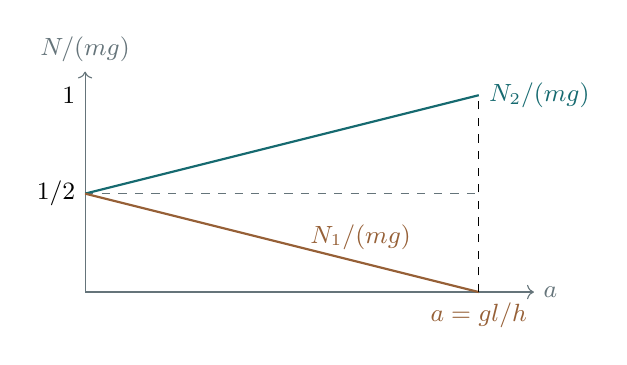
\begin{tikzpicture}[x=1cm,y=1cm]
\draw[->,color=muted] (0,0)--(5.7,0) node[right] {$a$};
\draw[->,color=muted] (0,0)--(0,2.8) node[above] {$N/(mg)$};
\draw[dashed,color=muted] (0,1.25)--(5,1.25);
\draw[thick,color=accent] (0,1.25)--(5,2.5) node[right] {$N_2/(mg)$};
\draw[thick,color=warm] (0,1.25)--(5,0) node[below] {$a=gl/h$};
\node[left] at (0,1.25) {$1/2$};\node[color=warm] at (3.5,.7) {$N_1/(mg)$};
\draw[dashed] (5,0)--(5,2.5);\node[left] at (0,2.5) {$1$};
\end{tikzpicture}
\figcaption{解图6.1B\quad 支持力随加速度作线性转移；右端是前轮刚离地的状态。}
\end{minipage}\end{center}
解图6.1B中两条斜线的和始终为1，说明竖直总支持力等于重力。后轮摩擦上限取上升载荷线对应的 $\mu N_2$，随加速度增加。

由后两式得 $N_2-N_1=mah/l$，与支持力之和联立：
\[
 N_1=\frac m2\left(g-\frac{ha}{l}\right),\qquad
 N_2=\frac m2\left(g+\frac{ha}{l}\right).
\]
后轮需要的驱动力为 $ma$，不滑动要求 $ma\le\mu N_2$，所以
\[\result{\mu\ge\frac{2la}{gl+ha}.}\]
这一结果以两轮都接地为前提，故还需 $a\le gl/h$（$h>0$）。当 $a=gl/h$ 时前轮支持力为零。再增大加速度，车身开始以前轮离地的姿态运动。负加速度使前轮增载、后轮减载；刹车时需按实际制动轮重新列摩擦条件。$h=0$ 时两轮各承担 $mg/2$，得到 $\mu\ge2a/g$。
\subsubsection*{路面给定时，先打滑还是先抬轮}
仍按解图6.1A的两轴接地模型，设$h>0$，把不打滑条件保持为未除式：
\[
(2l-\mu h)a\leq\mu gl,\qquad 0\leq a\leq\frac{gl}{h}.
\]
若$2l-\mu h>0$，才可直接除得摩擦给出的加速度上限
$a_f=\mu gl/(2l-\mu h)$。
比较$a_f$与解图6.1B前轮载荷降到零时的$a_w=gl/h$，有
\[
a_f\leq a_w\quad\Longleftrightarrow\quad\mu h\leq l.
\]
因此同时满足摩擦与接地的范围为
\[
0\leq a\leq a_{\max},\qquad
a_{\max}=\begin{cases}
\displaystyle\frac{\mu gl}{2l-\mu h},&0\leq\mu\leq l/h,\\[5pt]
\displaystyle\frac{gl}{h},&\mu\geq l/h.
\end{cases}
\]
在$\mu=l/h$时，两种临界状态同时到达：$N_1=0,N_2=mg$，
且$ma=\mu mg$。路面更粗糙时，前轮载荷首先降为零，两轮接地的平动过程在这里结束。
特别当$2l-\mu h\leq0$，摩擦不等式本身对非负$a$不再设上限，
此时两轮接地的加速度范围仍由 $a\leq gl/h$ 确定。

也可令$u=ah/(gl)$、$\kappa=\mu h/l$，
把两项条件化成$2u\leq\kappa(1+u)$与$0\leq u\leq1$。
两个无量纲条件在 $\kappa=1,u=1$ 处同时取等号。
当$h=0$时不使用含$1/h$的式子，而回到$N_1=N_2=mg/2$，
得到$a\leq\mu g/2$；此时加速度改变时，两个支持力始终各为 $mg/2$。


\Needspace{5\baselineskip}

\pdfbookmark[3]{关键洞察}{q1-h5}

\subsection*{关键洞察}

后轮接地处向前的摩擦力低于质心，对质心产生俯仰力矩。后轴增载、前轴减载产生反向力矩，保持车身的平动。加速时摩擦上限取后轴的实际载荷。

\Needspace{5\baselineskip}

\pdfbookmark[3]{易错点}{q1-h6}

\subsection*{易错点}

后轮的静摩擦向前，前轮的水平力在本题近似下为零。两个支持力的总和为 $mg$，差值为 $mah/l$；当算得前轮支持力降为零时，车身从两轴接地转入前轮离地过程。

\Needspace{5\baselineskip}

\pdfbookmark[3]{课堂讲解建议}{q1-h7}

\subsection*{课堂讲解建议}

在解图6.1A中逐一指出 $f,N_1,N_2$ 绕质心的转动方向，再问：“要抵消后轮摩擦的俯仰力矩，哪一轴增载？”用 $(N_2-N_1)l=mah$ 联系图上的箭头。沿解图6.1B增加加速度，让学生找到前轮支持力为零的位置，并比较它与摩擦达到上限的先后。计入车轮转动时，请学生指出整车角动量中随 $a/R$ 改变的自转部分，写进力矩方程。


\Needspace{5\baselineskip}

\pdfbookmark[3]{变式训练}{q1-h8}

\subsection*{变式训练}

\begin{enumerate}
\item 质心移向后轮。
\begin{center}\begin{minipage}{.98\linewidth}\centering
\begin{tikzpicture}[scale=.88,transform shape]
\draw[object](-2.8,0)--(2.8,0);
\draw[object](-2.35,.4)rectangle(2.35,1.55);
\foreach \x in {-2,2}{\draw[object](\x,.3)circle(.3);}
\fill(-0.65,1.15)circle(1.6pt)node[above]{$C$};
\draw[force](-2,0)--(-2,1.52)node[left]{$N_2$};
\draw[force](2,0)--(2,0.48)node[right]{$N_1$};
\draw[force](-0.65,1.15)--(-0.65,-.85)node[right]{$mg$};
\draw[force](-2,0)--(-1.4,0)node[below]{$f_2$};
\draw[motion](-.7,2)--(.7,2)node[right]{$a$};
\node[below]at(-2,-.5){后};\node[below]at(2,-.5){前};\draw[<->](-2,-1.15)--(-.65,-1.15)node[midway,below]{$d$};
\draw[<->](-2,-1.85)--(2,-1.85)node[midway,below]{$D$};
\end{tikzpicture}
\figcaption{变图6.1V1\quad 质心靠后时，静止后轴载荷较大}
\end{minipage}\end{center}
设后轮到质心的水平距离为 $d$、轮距为 $D$。竖直方向 $N_1+N_2=mg$，绕质心有 $mah+(D-d)N_1-dN_2=0$，解得
\[N_2=\frac{mg(D-d)+mah}{D},\qquad N_1=\frac{mgd-mah}{D}.\]
质心向后移动时，变图6.1V1 中的 $d$ 变小，后轴承担的支持力增大。同一加速度所需的驱动力仍为 $ma$，所以 $\mu_{\min}=ma/N_2$ 变小。两轴接地的条件是 $N_1\geq0$，即 $a\leq gd/h$（$h>0$）。
\item 改为前轮驱动。
\begin{center}\begin{minipage}{.98\linewidth}\centering
\begin{tikzpicture}[scale=.88,transform shape]
\draw[object](-2.8,0)--(2.8,0);
\draw[object](-2.35,.4)rectangle(2.35,1.55);
\foreach \x in {-2,2}{\draw[object](\x,.3)circle(.3);}
\fill(0,1.15)circle(1.6pt)node[above]{$C$};
\draw[force](-2,0)--(-2,1.3)node[left]{$N_2$};
\draw[force](2,0)--(2,0.7)node[right]{$N_1$};
\draw[force](0,1.15)--(0,-.85)node[right]{$mg$};
\draw[force](2,0)--(2.6,0)node[below]{$f_1$};
\draw[motion](-.7,2)--(.7,2)node[right]{$a$};
\node[below]at(-2,-.5){后};\node[below]at(2,-.5){前};
\end{tikzpicture}
\figcaption{变图6.1V2\quad 前轮驱动使用前轴的实际载荷}
\end{minipage}\end{center}
水平合力仍需 $ma$，变图6.1V2将它放在前轮。绕质心的水平力矩相同，故支持力仍按前式分配，而摩擦条件改为 $ma\leq\mu N_1$。当质心居中、$D=2l,d=l$，
\[\mu_{\min}=\frac{2la}{gl-ha},\qquad gl>ha.\]
前轴在加速时减载，前轮可用的摩擦随之减小。
\item 取 $h=0$。
\begin{center}\begin{minipage}{.98\linewidth}\centering
\begin{tikzpicture}[scale=.88,transform shape]
\draw[object](-2.5,0)--(2.5,0);
\fill(0,0)circle(1.8pt)node[above]{$C$};
\draw[force](0,0)--(0,-1.8)node[right]{$mg$};
\draw[force](-2,0)--(-2,.9)node[left]{$mg/2$};
\draw[force](2,0)--(2,.9)node[right]{$mg/2$};
\draw[force](-2,0)--(-1.2,0)node[below]{$ma$};
\node[above]at(0,1.5){质心与摩擦作用线同高};
\end{tikzpicture}
\figcaption{变图6.1V3\quad 水平驱动力通过质心高度，载荷均分}
\end{minipage}\end{center}
变图6.1V3的水平驱动力通过质心所在水平线，关于质心的力矩为零。由竖直合力与力矩得 $N_1=N_2=mg/2$。后轮承担全部水平驱动力，因此 $ma\leq\mu mg/2$，即 $\mu\geq2a/g$。
\item 给定 $\mu$ 求两轮接地的加速度上限。
\begin{center}\begin{minipage}{.98\linewidth}\centering
\begin{tikzpicture}[scale=.88,transform shape]
\begin{scope}[x=3cm,y=2.6cm]
\draw[axis](0,0)--(2.2,0)node[right]{$\kappa=\mu h/l$};
\draw[axis](0,0)--(0,1.3)node[above]{$a_{\max}h/(gl)$};
\draw[traj,domain=0:1,samples=65]plot(\x,{\x/(2-\x)});
\draw[traj](1,1)--(2,1);\draw[guide](1,0)--(1,1)--(0,1)node[left]{$1$};
\node[below]at(1,0){$1$};\node[anchor=west]at(1.12,.57){前轮离地};
\node[above left]at(.66,.49){摩擦达上限};\end{scope}
\end{tikzpicture}
\figcaption{变图6.1V4\quad 摩擦系数增大后，两轴接地的加速度上限趋于抬轮值}
\end{minipage}\end{center}
写成 $(2l-\mu h)a\leq\mu gl$，并同时取 $a\leq gl/h$。当 $0\leq\mu\leq l/h$，分母为正，摩擦先达到上限，$a_{\max}=\mu gl/(2l-\mu h)$。当 $\mu\geq l/h$，取 $a_{\max}=gl/h$。变图6.1V4中以 $\kappa=\mu h/l$ 为横坐标，在 $\kappa=1$ 处两种临界状态相遇；即使 $2l-\mu h\leq0$，两轴接地仍限定 $a\leq gl/h$。
\item 只用后轮制动，减速度大小为 $b$。
\begin{center}\begin{minipage}{.98\linewidth}\centering
\begin{tikzpicture}[scale=.88,transform shape]
\draw[object](-2.8,0)--(2.8,0);
\draw[object](-2.35,.4)rectangle(2.35,1.55);
\foreach \x in {-2,2}{\draw[object](\x,.3)circle(.3);}
\fill(0,1.15)circle(1.6pt)node[above]{$C$};
\draw[force](-2,0)--(-2,0.7)node[left]{$N_2$};
\draw[force](2,0)--(2,1.3)node[right]{$N_1$};
\draw[force](0,1.15)--(0,-.85)node[right]{$mg$};
\draw[force](-2,0)--(-2.6,0)node[below]{$f_2$};
\draw[motion](-.7,2)--(.7,2)node[right]{$-b$};
\node[below]at(-2,-.5){后};\node[below]at(2,-.5){前};\node[above]at(-2,2.5){后轮制动};
\end{tikzpicture}
\figcaption{变图6.1V5\quad 后轮制动时后轴减载}
\end{minipage}\end{center}
将水平加速度写为 $a=-b$，变图6.1V5中后轮摩擦向后、前轴支持力较大。由轴荷式，
\[N_1=\frac m2(g+hb/l),\quad N_2=\frac m2(g-hb/l),\quad mb\leq\mu N_2.\]
整理得 $b\leq\mu gl/(2l+\mu h)$，且后轮支持力为正。后轴减载使后轮能提供的制动力随减速度增加而减小。
\item 改为四轮驱动并理想分配驱动力。
\begin{center}\begin{minipage}{.98\linewidth}\centering
\begin{tikzpicture}[scale=.88,transform shape]
\draw[object](-2.8,0)--(2.8,0);
\draw[object](-2.35,.4)rectangle(2.35,1.55);
\foreach \x in {-2,2}{\draw[object](\x,.3)circle(.3);}
\fill(0,1.15)circle(1.6pt)node[above]{$C$};
\draw[force](-2,0)--(-2,1.3)node[left]{$N_2$};
\draw[force](2,0)--(2,0.7)node[right]{$N_1$};
\draw[force](0,1.15)--(0,-.85)node[right]{$mg$};
\draw[force](-2,0)--(-1.6099999999999999,0)node[below]{$f_2$};\draw[force](2,0)--(2.21,0)node[below]{$f_1$};
\draw[motion](-.7,2)--(.7,2)node[right]{$a$};
\node[below]at(-2,-.5){后};\node[below]at(2,-.5){前};
\end{tikzpicture}
\figcaption{变图6.1V6\quad 按两个轴载荷分配驱动力}
\end{minipage}\end{center}
变图6.1V6将总驱动力分给两个轴，取 $f_i=(N_i/mg)ma$，每个接触都满足 $f_i/N_i=a/g$。总静摩擦上限为 $\mu(N_1+N_2)=\mu mg$，因此 $a\leq\mu g$，两轴接地同时给出 $a\leq gl/h$。这种分配在两个轴上同时使用同一比例的静摩擦。
\item 计入车轮自转惯量。
\begin{center}\begin{minipage}{.98\linewidth}\centering
\begin{tikzpicture}[scale=.88,transform shape]
\draw[object](-2.8,0)--(2.8,0);
\draw[object](-2.35,.4)rectangle(2.35,1.55);
\foreach \x in {-2,2}{\draw[object](\x,.3)circle(.3);}
\fill(0,1.15)circle(1.6pt)node[above]{$C$};
\draw[force](-2,0)--(-2,1.38)node[left]{$N_2$};
\draw[force](2,0)--(2,0.62)node[right]{$N_1$};
\draw[force](0,1.15)--(0,-.85)node[right]{$mg$};
\draw[force](-2,0)--(-1.3,0)node[below]{$f_2$};\draw[force](2,0)--(1.9,0)node[below]{$f_1$};
\draw[motion](-.7,2)--(.7,2)node[right]{$a$};
\node[below]at(-2,-.5){后};\node[below]at(2,-.5){前};\draw[motion](-2.2,.53)arc(130:-150:.29);\draw[motion](1.8,.53)arc(130:-150:.29);
\node[above]at(0,2.55){两轮角加速度为顺时针};
\end{tikzpicture}
\figcaption{变图6.1V7\quad 前轮由向后的静摩擦取得自转角加速度}
\end{minipage}\end{center}
前、后轮总惯量分别为 $I_f,I_r$，半径同为 $R$。变图6.1V7中车轮向右加速滚动，角加速度顺时针，大小为 $a/R$。前轮靠向后的摩擦得到该角加速度，故 $f_1=-I_fa/R^2$。总水平力为 $ma$，后轮需 $f_2=ma+I_fa/R^2$。整车绕质心的自转角动量变化率是 $-(I_f+I_r)a/R$，因此
\[
mah+l(N_1-N_2)=-\frac{(I_f+I_r)a}{R},\qquad
N_2-N_1=\frac{mah+(I_f+I_r)a/R}{l}.
\]
结合 $N_1+N_2=mg$ 求实际轴荷，再比较 $f_2\leq\mu N_2$；若也给前轮摩擦系数，还应比较 $|f_1|$ 与相应上限。
\item 同时画出加速与制动时的载荷趋势。
\begin{center}\begin{minipage}{.98\linewidth}\centering
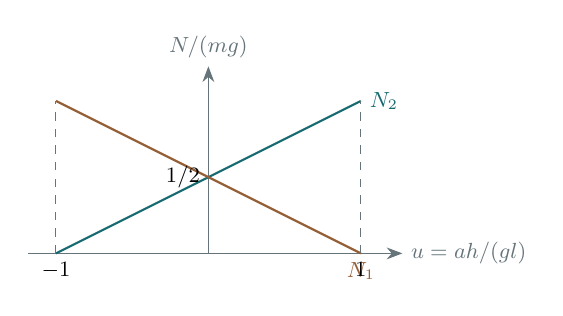
\begin{tikzpicture}[scale=.88,transform shape]
\draw[axis](-2.6,0)--(2.8,0)node[right]{$u=ah/(gl)$};
\draw[axis](0,0)--(0,2.7)node[above]{$N/(mg)$};
\draw[traj](-2.2,0)--(2.2,2.2)node[right]{$N_2$};
\draw[force,-](-2.2,2.2)--(2.2,0)node[below]{$N_1$};
\draw[guide](-2.2,0)--(-2.2,2.2);\draw[guide](2.2,0)--(2.2,2.2);
\node[left]at(0,1.1){$1/2$};\node[below]at(-2.2,0){$-1$};\node[below]at(2.2,0){$1$};
\end{tikzpicture}
\figcaption{变图6.1V8\quad 正加速度使后轴增载，负加速度使前轴增载}
\end{minipage}\end{center}
令有符号加速度参数 $u=ah/(gl)$。由 $(N_2-N_1)l=mah$ 及支持力之和，得到 $N_2/(mg)=(1+u)/2$、$N_1/(mg)=(1-u)/2$。变图6.1V8左半段对应制动，前轴增载；右半段对应加速，后轴增载。图的两端分别有一个支持力降为零，两轴接地取 $-1\leq u\leq1$。
\end{enumerate}

\clearpage

\pdfbookmark[2]{第 2 题 均匀圆柱体绕斜向质心轴的转动惯量}{q2}

\section*{第 2 题\quad 均匀圆柱体绕斜向质心轴的转动惯量}

\tagline{M-06-02}

如图6.2,质量为\(m\)的均匀圆柱体,截面半径为\(R\),长为\(2R\).试求:圆柱体绕通过质心及两底面边缘的转轴(图6.2中的\(\sigma_{1}\)或\(\sigma_{2}\))的转动惯量.

\begin{center}\begin{minipage}{\linewidth}\centering
\begin{tikzpicture}[font=\small]
\draw[object](-1.5,-1.5)rectangle(1.5,1.5);
\draw[axis](-2.4,0)--(2.5,0)node[right]{$\sigma_3$};
\draw[axis](0,-2.15)--(0,2.15)node[above]{$\sigma_4$};
\draw[axis](-2,-2)--(2,2)node[above right]{$\sigma_1$};
\draw[axis](-2,2)--(2,-2)node[below right]{$\sigma_2$};
\fill(0,0)circle(1.7pt);\node at(.35,-.65){$O$};
\draw[<->](-1.5,-2.65)--(1.5,-2.65)node[midway,below]{$2R$};
\draw[<->](-2.55,0)--(-2.55,1.5)node[midway,left]{$R$};
\node at(0,-3.5){中轴所在截面；$\sigma_5$垂直图面};
\end{tikzpicture}
\figcaption{图 6.2\quad 长与直径相等；对角轴穿过质心及两底面边缘。}
\end{minipage}\end{center}

\Needspace{5\baselineskip}

\pdfbookmark[3]{题型定位}{q2-h0}

\subsection*{题型定位}

三维正交轴惯量和、薄片垂直轴定理与平行轴积分。

\Needspace{5\baselineskip}

\pdfbookmark[3]{知识点}{q2-h1}

\subsection*{知识点}

\begin{itemize}
\tightlist
\item
  转动惯量定义
\item
  薄片垂直轴定理与三维正交轴惯量和
\item
  平行轴定理
\item
  薄圆片积分
\item
  对称轴选择
\end{itemize}

过同一点的三根正交轴的惯量和等于$2\int r^2\dd m$，旋转轴组不改变该和。圆柱对称轴与横向主轴的惯量可用主惯量投影组合；只有过同一原点时才可直接比较，平移轴线需另用平行轴定理。


\Needspace{5\baselineskip}

\pdfbookmark[3]{物理图像}{q2-h2}

\subsection*{物理图像}

解图6.2A是含圆柱中轴的截面。长与直径相等，截面为正方形，两条对角轴相互垂直；镜面对称又使它们的惯量相等。解图6.2B在位置 $x$ 切出圆片，圆片直径轴到整体横轴的距离为 $|x|$。

\Needspace{5\baselineskip}

\pdfbookmark[3]{解题入口}{q2-h3}

\subsection*{解题入口}

先证任意三维物体的正交轴惯量和，再比较两组轴。薄圆片才可以使用通常的垂直轴定理。

将薄圆片的自身直径轴惯量和平行轴项相加，积分得到横向质心轴惯量，再代正交轴和关系。

\Needspace{5\baselineskip}

\pdfbookmark[3]{标准解法}{q2-h4}

\subsection*{标准解法}

\begin{center}\begin{minipage}{\linewidth}\centering
\begin{tikzpicture}[font=\small]
\draw[object](-1.5,-1.5)rectangle(1.5,1.5);
\draw[axis](-2.4,0)--(2.5,0)node[right]{$\sigma_3$};
\draw[axis](0,-2.15)--(0,2.15)node[above]{$\sigma_4$};
\draw[axis](-2,-2)--(2,2)node[above right]{$\sigma_1$};
\draw[axis](-2,2)--(2,-2)node[below right]{$\sigma_2$};
\fill(0,0)circle(1.7pt);\node at(.35,-.65){$O$};
\draw[<->](-1.5,-2.65)--(1.5,-2.65)node[midway,below]{$2R$};
\draw[<->](-2.55,0)--(-2.55,1.5)node[midway,left]{$R$};
\node at(0,-3.5){中轴所在截面；$\sigma_5$垂直图面};
\end{tikzpicture}
\figcaption{解图 6.2A\quad 两组过同一原点的正交轴有相同惯量和。}
\end{minipage}\end{center}
圆柱长为 $2R$，故解图6.2A中的两条对角轴 $\sigma_1,\sigma_2$ 相互垂直，与中轴均成 $45^\circ$；$\sigma_5$ 垂直这个轴平面。先证明适用于三维物体的正交轴和关系。质元坐标为 $(x_i,y_i,z_i)$ 时，
\[
\begin{aligned}
 I_x&=\sum_i\Delta m_i(y_i^2+z_i^2),\\
 I_y&=\sum_i\Delta m_i(z_i^2+x_i^2),\\
 I_z&=\sum_i\Delta m_i(x_i^2+y_i^2).
\end{aligned}
\]
相加得到 $I_x+I_y+I_z=2\sum_i\Delta m_i r_i^2$。同一原点下，该和与正交轴组的朝向无关。因此
\[
 I_1+I_2+I_5=I_3+I_4+I_5,\qquad
 2I=I_3+I_4=\frac12mR^2+I_4.
\]
上式中的$I_1=I_2$还用了圆柱的镜面对称性：将圆柱关于横向中面反射，
解图6.2A的$\sigma_1,\sigma_2$互换，而质量分布不变。
也可从中轴、横向轴这两条主轴直接投影：
\[
I(\alpha)=I_3\cos^2\alpha+I_4\sin^2\alpha.
\]
混合惯量积分因镜面对称为零；本题$\alpha=45^\circ$，两项权重各为$1/2$，
所以才可把$I_1+I_2$写成$2I$。
本题的两条斜轴相互垂直，可以与 $\sigma_5$ 组成一组正交轴。若改变柱长，可直接用投影式分别求两条斜轴的惯量。

圆柱的三维轴和使用三个坐标的平方；圆片的垂直轴关系在下面单独用于每一薄片。

\begin{center}\begin{minipage}{\linewidth}\centering
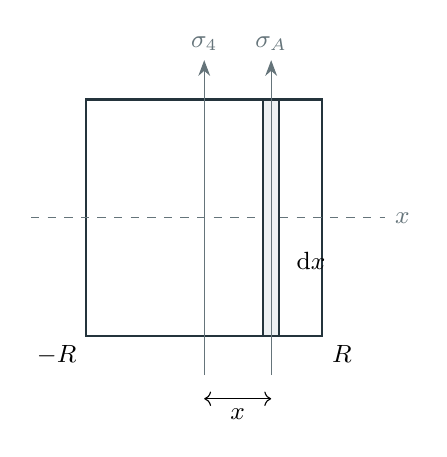
\begin{tikzpicture}[font=\small]
\draw[object](-1.5,-1.5)rectangle(1.5,1.5);
\draw[guide](-2.2,0)--(2.3,0)node[right]{$x$};
\draw[object,fill=rulegray!40](.75,-1.5)rectangle(.95,1.5);
\draw[axis](0,-2)--(0,2)node[above]{$\sigma_4$};
\draw[axis](.85,-2)--(.85,2)node[above]{$\sigma_A$};
\draw[<->](0,-2.3)--(.85,-2.3)node[midway,below]{$x$};
\node[right]at(1.05,-.55){$\dd x$};
\node[below left]at(-1.5,-1.5){$-R$};\node[below right]at(1.5,-1.5){$R$};
\end{tikzpicture}
\figcaption{解图 6.2B\quad 薄圆片先求直径轴惯量，再平移 $|x|$ 到圆柱横向质心轴。}
\end{minipage}\end{center}
解图6.2B在中轴坐标 $x$ 处切出厚度 $\dd x$ 的薄圆片，其质量 $\dd m=m\dd x/(2R)$。薄片轴向惯量为 $\dd I_C=\dd mR^2/2$；薄片的两条直径轴等价，且垂直轴定理给 $\dd I_C=2\dd I_A$，故
\[
 \dd I_A=\frac14R^2\dd m=\frac{mR}{8}\dd x.
\]
将薄片直径轴平移至整个圆柱的横向质心轴，距离为 $|x|$：
\[
 \dd I_4=\dd I_A+x^2\dd m
 =\frac{mR}{8}\dd x+\frac{m}{2R}x^2\dd x.
\]
积分并代回轴和关系：
\[
\begin{aligned}
 I_4&=\frac{mR}{8}\int_{-R}^{R}\dd x+
 \frac{m}{2R}\int_{-R}^{R}x^2\dd x
 =\frac14mR^2+\frac13mR^2=\frac7{12}mR^2,\\
 I&=\frac12\left(\frac12+\frac7{12}\right)mR^2
 =\result{\frac{13}{24}mR^2}.
\end{aligned}
\]
从主惯量投影看，轴向主惯量为 $mR^2/2$，横向为 $7mR^2/12$，斜轴惯量是二者按 $\cos^245^\circ$、$\sin^245^\circ$ 加权之和。
\subsubsection*{三维轴和与薄圆片的径向积分}
三维轴和关系中，$r_i^2=x_i^2+y_i^2+z_i^2$ 是质元到公共原点 $O$ 的距离平方。每条转轴的惯量由垂直于该轴的两个坐标平方组成，将三个定义式逐项相加，得到
\[
\begin{aligned}
I_x+I_y+I_z
&=\sum_i\Delta m_i[(y_i^2+z_i^2)+(z_i^2+x_i^2)+(x_i^2+y_i^2)]\\
&=2\sum_i\Delta m_i(x_i^2+y_i^2+z_i^2)
=2\sum_i\Delta m_i r_i^2.
\end{aligned}
\]
转动坐标轴不改变$r_i$，故对解图6.2A的两组轴分别有
\[
I_1+I_2=2\sum_i\Delta m_i r_i^2-I_5,
\qquad
I_3+I_4=2\sum_i\Delta m_i r_i^2-I_5.
\]
两边相减才得到$I_1+I_2=I_3+I_4$。
各轴通过同一点、每组三轴两两正交时，这一证明对三维物体和薄片、均匀与非均匀质量分布都成立。

薄圆片的垂直轴定理则用在解图6.2C所示的局部圆面上。
该片内两条直径轴为$\sigma_A,\sigma_B$，
面法线轴为$\sigma_C$；忽略$\dd x$厚度的高阶效应，
质元到面法线的距离平方恰为到两条面内轴的距离平方之和，因而
\[
\dd I_C=\dd I_A+\dd I_B,
\qquad \dd I_A=\dd I_B.
\]
\begin{center}\begin{minipage}{\linewidth}\centering
\begin{tikzpicture}
\draw[object](0,0)circle(1.3);
\draw[axis](-1.8,0)--(1.9,0)node[right]{$\sigma_B$};
\draw[axis](0,-1.8)--(0,1.9)node[above]{$\sigma_A$};
\node[fill=white,inner sep=1pt]at(0,0){$\odot$};
\node[above left]at(-.12,.12){$O_A$};
\fill(.8,.45)circle(1.6pt)node[above right]{$\delta m$};
\draw[guide](.8,0)--(.8,.45)--(0,.45);
\draw[<->](0,0)--(-.919238816,-.919238816)node[midway,below left]{$R$};
\node[align=left,anchor=west]at(2.8,.7){$\sigma_C$垂直圆面\\$\dd I_C=\dd I_A+\dd I_B$\\两条直径轴因对称而等价};
\end{tikzpicture}
\figcaption{解图6.2C\quad 薄圆片的三条局部轴；圆面上的$\delta m$用于解释垂直轴关系。}
\end{minipage}\end{center}
圆片的面密度为$\dd m/(\pi R^2)$。
把圆片再分成半径$s$、宽$\dd s$的圆环，
圆环质量为$2\dd m\,s\dd s/R^2$，所以
\[
\dd I_C=\int_0^R s^2\frac{2\dd m}{R^2}s\dd s
=\frac12R^2\dd m.
\]
由解图6.2B中均匀圆柱的轴向质量分配$\dd m=m\dd x/(2R)$，
逐步代入可得
\[
\dd I_C=\frac12\frac{m}{2R}\dd x\,R^2
=\frac{mR}{4}\dd x,
\qquad
\dd I_A=\frac12\dd I_C=\frac{mR}{8}\dd x.
\]
薄片绕自身直径轴已有惯量 $\dd I_A$，平移后再加 $x^2\dd m$，两项共同组成薄片对 $\sigma_4$ 的惯量。
两项积分的边界和数值分别是
\[
\begin{aligned}
\int_{-R}^{R}\frac{mR}{8}\dd x
&=\frac{mR}{8}[x]_{-R}^{R}=\frac14mR^2,\\
\int_{-R}^{R}\frac{m}{2R}x^2\dd x
&=\frac{m}{2R}\left[\frac{x^3}{3}\right]_{-R}^{R}
=\frac13mR^2.
\end{aligned}
\]
于是$I_4=7mR^2/12$，再由$2I=mR^2/2+I_4$还原
\[
I=\frac14mR^2+\frac12I_4
=\left(\frac14+\frac7{24}\right)mR^2
=\frac{13}{24}mR^2.
\]
所求值介于中轴惯量$12mR^2/24$与横轴惯量$14mR^2/24$之间，
符合$45^\circ$主轴投影的等权结果。
解图6.2A、B的轴向截面均按边长$2R$的正方形绘制，
薄片坐标$x$与轴间平移距离$|x|$在同一几何比例下对应。


\Needspace{5\baselineskip}

\pdfbookmark[3]{关键洞察}{q2-h5}

\subsection*{关键洞察}

两组正交轴通过同一原点时，惯量和相等。对称性给两条斜轴惯量相等；横向轴惯量则由薄片自身惯量与平行轴项积分得到。

正交轴和不依赖轴组朝向，单个惯量则依赖。薄片自身惯量和平行轴项各贡献 $mR^2/4$ 和 $mR^2/3$。

\Needspace{5\baselineskip}

\pdfbookmark[3]{易错点}{q2-h6}

\subsection*{易错点}

三维圆柱使用三轴惯量和 $2\int r^2\dd m$，圆片使用面内两条轴与面法线的垂直轴关系。薄片对整体横轴的惯量包括自身直径惯量和平行轴项。改变圆柱长度时，两条对角线夹角随之改变。

\Needspace{5\baselineskip}

\pdfbookmark[3]{课堂讲解建议}{q2-h7}

\subsection*{课堂讲解建议}

让学生在解图6.2A中指出两组正交轴，并用一粒质元的三个垂距平方解释轴和相同。在解图6.2C上再看同一粒质元，问：“薄圆片的面内轴垂距平方相加，得到哪条轴的垂距平方？”随后在解图6.2B读出两条平行轴之间的 $|x|$，分别积分圆片自身项与平移项。


\Needspace{5\baselineskip}

\pdfbookmark[3]{变式训练}{q2-h8}

\subsection*{变式训练}

\begin{enumerate}
\item 圆柱长度改为 $H$。
\begin{center}\begin{minipage}{.98\linewidth}\centering
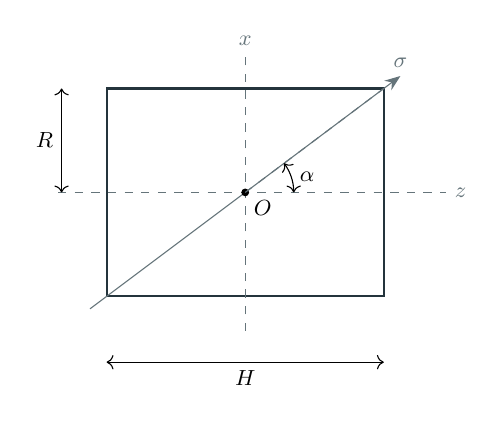
\begin{tikzpicture}[scale=.88,transform shape]
\draw[object](-2.0,-1.5)rectangle(2.0,1.5);
\draw[guide](-2.7,0)--(2.9,0)node[right]{$z$};
\draw[guide](0,-2)--(0,2)node[above]{$x$};
\draw[axis](-2.23999999987814,-1.6800000001624795)--(2.23999999987814,1.6800000001624795)node[above]{$\sigma$};
\fill(0,0)circle(1.6pt)node[below right]{$O$};
\draw[<->](-2.0,-2.45)--(2.0,-2.45)node[midway,below]{$H$};
\draw[<->](-2.65,0)--(-2.65,1.5)node[midway,left]{$R$};
\draw[guide](0,0)--(2,1.5);\draw[<->](.7,0)arc(0:36.86989765:.7)node[midway,right]{$\alpha$};
\end{tikzpicture}
\figcaption{变图6.2V1\quad 任意长度时，斜轴角度由截面长宽确定}
\end{minipage}\end{center}
变图6.2V1中，质心到边缘的横向距离为 $R$、轴向距离为 $H/2$，故 $\tan\alpha=2R/H$。均匀圆柱的主惯量为
\[I_z=\frac12mR^2,\qquad I_x=m\left(\frac{R^2}{4}+\frac{H^2}{12}\right).\]
横向项可把薄片直径惯量 $\dd mR^2/4$ 与轴向位置项 $z^2\dd m$ 从 $-H/2$ 积到 $H/2$ 得到。斜轴惯量是 $I=I_z\cos^2\alpha+I_x\sin^2\alpha$。
\item 求底面直径轴的惯量。
\begin{center}\begin{minipage}{.98\linewidth}\centering
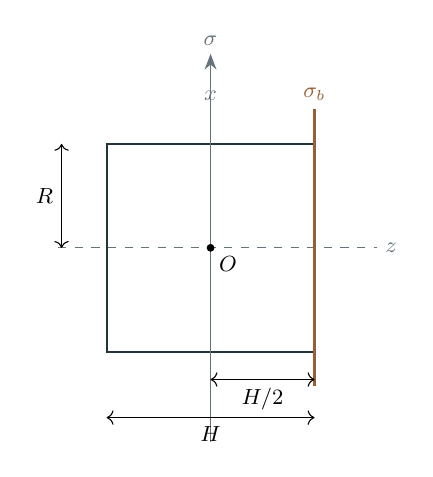
\begin{tikzpicture}[scale=.88,transform shape]
\draw[object](-1.5,-1.5)rectangle(1.5,1.5);
\draw[guide](-2.2,0)--(2.4,0)node[right]{$z$};
\draw[guide](0,-2)--(0,2)node[above]{$x$};
\draw[axis](-1.7145055188062944e-16,-2.8)--(1.7145055188062944e-16,2.8)node[above]{$\sigma$};
\fill(0,0)circle(1.6pt)node[below right]{$O$};
\draw[<->](-1.5,-2.45)--(1.5,-2.45)node[midway,below]{$H$};
\draw[<->](-2.15,0)--(-2.15,1.5)node[midway,left]{$R$};
\draw[force,-](1.5,-2)--(1.5,2)node[above]{$\sigma_b$};\draw[<->](0,-1.9)--(1.5,-1.9)node[midway,below]{$H/2$};
\end{tikzpicture}
\figcaption{变图6.2V2\quad 底面直径轴与质心横轴相隔半个柱长}
\end{minipage}\end{center}
变图6.2V2中的 $\sigma_b$ 与横向质心轴平行，距离为 $H/2$。平行轴定理给
\[I_b=I_x+m(H/2)^2=m\left(\frac{R^2}{4}+\frac{H^2}{3}\right).\]
取 $H=2R$，得 $I_b=19mR^2/12$。
\item 直接用质元到斜轴的距离积分。
\begin{center}\begin{minipage}{.98\linewidth}\centering
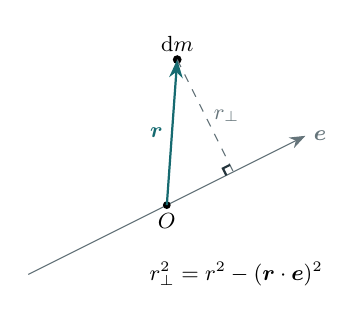
\begin{tikzpicture}[scale=.88,transform shape]
\draw[axis](-2,-1)--(2,1)node[right]{$\boldsymbol e$};
\fill(0,0)circle(1.6pt)node[below]{$O$};
\fill(.15,2.1)circle(1.8pt)node[above]{$\dd m$};
\draw[motion](0,0)--(.15,2.1)node[midway,left]{$\boldsymbol r$};
\draw[guide](.15,2.1)--(.96,.48)node[midway,right]{$r_\perp$};
\draw[object](.86,.43)--(.81,.53)--(.91,.58);
\node[below]at(1,-.7){$r_\perp^2=r^2-(\boldsymbol r\cdot\boldsymbol e)^2$};
\end{tikzpicture}
\figcaption{变图6.2V3\quad 质元到斜轴的垂距决定其惯量}
\end{minipage}\end{center}
变图6.2V3中，斜轴单位向量为 $\boldsymbol e=(\sin\alpha,0,\cos\alpha)$。代入
\[I=\int[r^2-(\boldsymbol r\cdot\boldsymbol e)^2]\dd m,\]
展开后得到 $\cos^2\alpha\int(x^2+y^2)\dd m+\sin^2\alpha\int(y^2+z^2)\dd m-2\sin\alpha\cos\alpha\int xz\dd m$。镜面对称使最后一项为零，剩下主惯量投影式。
\item 换成均匀薄壁圆筒。
\begin{center}\begin{minipage}{.98\linewidth}\centering
\begin{tikzpicture}[scale=.88,transform shape]
\draw[object](-1.5,-1.5)rectangle(1.5,1.5);
\draw[guide](-2.2,0)--(2.4,0)node[right]{$z$};
\draw[guide](0,-2)--(0,2)node[above]{$x$};
\draw[axis](-1.9798989873223332,-1.9798989873223327)--(1.9798989873223332,1.9798989873223327)node[above]{$\sigma$};
\fill(0,0)circle(1.6pt)node[below right]{$O$};
\draw[<->](-1.5,-2.45)--(1.5,-2.45)node[midway,below]{$H$};
\draw[<->](-2.15,0)--(-2.15,1.5)node[midway,left]{$R$};
\draw[traj](-1.5,-1.5)--(1.5,-1.5);\draw[traj](-1.5,1.5)--(1.5,1.5);\node[above]at(0,2.6){侧壁质量，底面忽略};
\end{tikzpicture}
\figcaption{变图6.2V4\quad 薄壁圆筒的轴向与横向惯量}
\end{minipage}\end{center}
变图6.2V4中质量均在半径 $R$ 的侧面，故 $I_z=mR^2$。横轴的径向贡献为 $mR^2/2$，轴向均匀分布贡献为 $mH^2/12$，所以 $I_x=m(R^2/2+H^2/12)$。在 $H=2R,\alpha=45^\circ$ 时，两项各取一半，得 $I=11mR^2/12$。
\item 比较同一方向的平移轴。
\begin{center}\begin{minipage}{.98\linewidth}\centering
\begin{tikzpicture}[scale=.88,transform shape]
\draw[axis](-2,-1)--(2,1)node[right]{$\sigma_C$};
\draw[axis](-2,.3)--(2,2.3)node[right]{$\sigma'$};
\fill(0,0)circle(1.7pt)node[below]{$C$};
\draw[<->](.4,.2)--(-.12,1.24)node[midway,right]{$d$};
\node[below]at(0,-1.6){两轴方向相同};
\end{tikzpicture}
\figcaption{变图6.2V5\quad 平行轴项使用两轴之间的最短距离}
\end{minipage}\end{center}
沿变图6.2V5中两轴的公垂线取坐标，质元到新轴的距离平方展开有质心惯量、$md^2$ 和一阶矩项。质心的一阶矩为零，故 $I'=I_C+md^2$。相同方向的轴以过质心时惯量最小；方向改变时使用主惯量投影比较。
\item 保持 $H=2R$，只改变斜轴角度。
\begin{center}\begin{minipage}{.98\linewidth}\centering
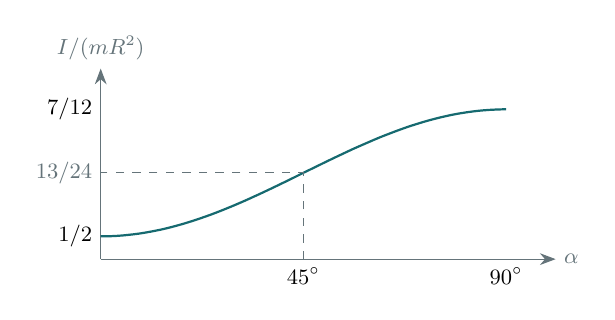
\begin{tikzpicture}[scale=.88,transform shape]
\begin{scope}[x=.065cm,y=22cm]
\draw[axis](0,.485)--(101,.485)node[right]{$\alpha$};
\draw[axis](0,.485)--(0,.61)node[above]{$I/(mR^2)$};
\draw[traj,domain=0:90,samples=75]plot(\x,{.5*cos(\x)^2+7*sin(\x)^2/12});
\draw[guide](45,.485)--(45,{13/24})--(0,{13/24})node[left]{$13/24$};
\node[left]at(0,.5){$1/2$};\node[left]at(0,{7/12}){$7/12$};
\node[below]at(45,.485){$45^\circ$};\node[below]at(90,.485){$90^\circ$};\end{scope}
\end{tikzpicture}
\figcaption{变图6.2V6\quad 斜轴方向从中轴逐渐转向横轴}
\end{minipage}\end{center}
变图6.2V6绘出
\[I=mR^2\left(\frac12\cos^2\alpha+\frac7{12}\sin^2\alpha\right)=mR^2\left(\frac12+\frac1{12}\sin^2\alpha\right).\]
在 $0\leq\alpha\leq\pi/2$，导数为 $mR^2\sin(2\alpha)/12\geq0$。曲线从 $mR^2/2$ 上升到 $7mR^2/12$，在 $45^\circ$ 取 $13mR^2/24$。
\item 轴对称圆柱的密度不均匀。
\begin{center}\begin{minipage}{.98\linewidth}\centering
\begin{tikzpicture}[scale=.88,transform shape]
\draw[object](0,0)circle(1.5);
\draw[object](0,0)circle(.8);\draw[object](0,0)circle(1.05);
\fill[accent!15](0,0)circle(1.05);\fill[white](0,0)circle(.8);
\draw[axis](0,0)--(2.1,0)node[right]{$s$};
\draw[<->](.8,-.15)--(1.05,-.15)node[below right]{$\dd s$};
\node[above]at(0,1.9){密度 $\rho(s,z)$};
\node[below]at(0,-1.9){按圆环与轴向位置积分};
\end{tikzpicture}
\figcaption{变图6.2V7\quad 轴对称密度依赖离轴距离与轴向坐标}
\end{minipage}\end{center}
变图6.2V7以圆环坐标 $s$ 和轴向坐标 $z$ 描述密度。轴对称且关于质心横面对称时，主惯量为
\[I_z=\int s^2\dd m,\qquad I_x=\int(s^2/2+z^2)\dd m.\]
若仅轴对称，取 $z=0$ 为质心横面后，积分的混合项仍因方位角平均为零。代入 $I=I_z\cos^2\alpha+I_x\sin^2\alpha$ 求斜轴惯量。三根正交轴的惯量和 $2\int r^2\dd m$ 对这些密度同样成立。
\item 长度改变后，比较两条对角轴的夹角和惯量。
\begin{center}\begin{minipage}{.98\linewidth}\centering
\begin{tikzpicture}[scale=.88,transform shape]
\draw[object](-2.0,-1.5)rectangle(2.0,1.5);
\draw[guide](-2.7,0)--(2.9,0)node[right]{$z$};
\draw[guide](0,-2)--(0,2)node[above]{$x$};
\draw[axis](-2.24,-1.68)--(2.24,1.68)node[above right]{$\sigma_1$};
\fill(0,0)circle(1.6pt)node[below right]{$O$};
\draw[<->](-2.0,-2.45)--(2.0,-2.45)node[midway,below]{$H$};
\draw[<->](-2.65,0)--(-2.65,1.5)node[midway,left]{$R$};
\draw[axis](-2,1.5)--(2,-1.5)node[right]{$\sigma_2$};\node[above]at(0,2.6){两个斜轴关于中轴对称};
\end{tikzpicture}
\figcaption{变图6.2V8\quad 长度改变后，对称斜轴仍有相同惯量}
\end{minipage}\end{center}
变图6.2V8中两轴方向可取 $(H/2,R)$ 与 $(H/2,-R)$。它们的点积是 $H^2/4-R^2$，在 $H=2R$ 时为零。长度取其他值时两轴夹角改变，镜面对称仍使惯量相同，因为投影式中出现 $\cos^2\alpha$、$\sin^2\alpha$。
\end{enumerate}

\clearpage

\pdfbookmark[2]{第 3 题 桌边细杆开始滑动的临界角}{q3}

\section*{第 3 题\quad 桌边细杆开始滑动的临界角}

\tagline{M-06-03}

如图,长为\(l\)的均匀细杆水平地放置在桌面上,质心离桌边缘的距离为\(b\),从静止下落.

已知杆与桌边缘之间的摩擦系数为 \(\mu\). 试求杆开始滑动时 的角度
\(\theta_{C}\).

\begin{center}\begin{minipage}{\linewidth}\centering
\begin{tikzpicture}[font=\small]
\draw[object](-2,0)--(0,0)--(0,-2);\draw[object,line width=2pt](-1.3,0)--(3.5,0);\fill(0,0)circle(2pt)node[below left]{$A$};\fill(1.1,0)circle(2pt)node[above]{$C$};\draw[<->](0,.6)--(1.1,.6)node[midway,above]{$b$};\node[below]at(2.8,-.2){杆长 $l$};
\end{tikzpicture}
\figcaption{图 6.3\quad 质心在桌边外侧；初态水平静止。}
\end{minipage}\end{center}

\Needspace{5\baselineskip}

\pdfbookmark[3]{题型定位}{q3-h0}

\subsection*{题型定位}

桌边杆的定轴转动与静摩擦约束失效。

\Needspace{5\baselineskip}

\pdfbookmark[3]{知识点}{q3-h1}

\subsection*{知识点}

\begin{itemize}
\tightlist
\item
  定轴转动
\item
  质心加速度
\item
  桌边支持力与摩擦
\item
  能量求角速度
\item
  滑动临界
\end{itemize}

开始滑动前桌角可作为暂时固定转轴，角速度由机械能确定。质心同时有切向和向心加速度，接触力分解后才可求摩擦与支持力。起滑时所需摩擦达到上限，桌角仍施加正的支持力。杆从水平静止开始转下还需重力对桌角有力矩。


\Needspace{5\baselineskip}

\pdfbookmark[3]{物理图像}{q3-h2}

\subsection*{物理图像}

解图6.3A中 $A$ 是尚未滑动的接触点，质心在外侧，与它相距 $b$。摩擦沿杆指向 $A$，一部分抵消重力沿杆的分量，一部分提供向心加速度。支持力垂直杆，与重力的垂杆分量之差产生切向加速度。

\Needspace{5\baselineskip}

\pdfbookmark[3]{解题入口}{q3-h3}

\subsection*{解题入口}

在未滑动阶段，把 A
点视为固定轴。先由能量求角速度随角度的关系，再由转动动力学和质心加速度求桌边压力与摩擦，最后令摩擦达到临界。

绕 $A$ 求角加速度，积分或能量求角速度，再沿杆及垂直杆求 $f,N$。由 $f/N$ 随倾角单调增大，取它第一次等于静摩擦系数的角度。

\Needspace{5\baselineskip}

\pdfbookmark[3]{标准解法}{q3-h4}

\subsection*{标准解法}

\begin{center}\begin{minipage}{\linewidth}\centering
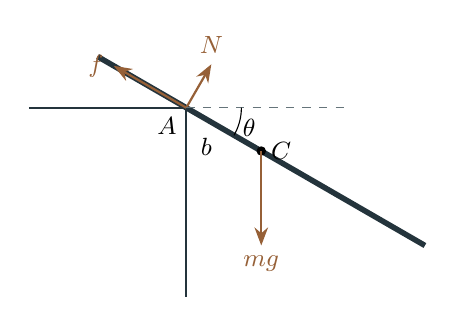
\begin{tikzpicture}[font=\small]
\draw[object](-2,0)--(0,0)--(0,-2.4);
\draw[object,line width=2pt](-1.125833025,.65)--(3.031088913,-1.75);
\coordinate(C)at(.952627944,-.55);
\node[below left]at(0,0){$A$};\fill(C)circle(1.7pt)node[right]{$C$};
\draw[force](0,0)--(-.921362490,.531948882)node[left]{$f$};
\draw[force](0,0)--(.318741618,.552076677)node[above]{$N$};
\draw[force](C)--++(0,-1.2)node[below]{$mg$};
\draw[guide](0,0)--(2,0);\draw(.7,0)arc(0:-30:.7);
\node at(.8,-.25){$\theta$};\node[below left]at(.45,-.26){$b$};
\end{tikzpicture}
\figcaption{解图 6.3A\quad 桌角摩擦沿杆，支持力垂直杆；质心同时有切向和向心加速度。}
\end{minipage}\end{center}
杆的质心 $C$ 在桌边 $A$ 外侧，$AC=b>0$。解图6.3A取转下角 $\theta$ 为正，摩擦 $f$ 沿杆指向 $A$，支持力 $N$ 垂直杆；不滑动时 $A$ 固定。令
\[
 I_C=\frac1{12}ml^2,\quad I_A=I_C+mb^2,\quad \beta=\dot\omega.
\]
绕 $A$ 的重力矩给 $I_A\beta=mgb\cos\theta$。质心法向、切向方程为
\[
 f-mg\sin\theta=mb\omega^2,\qquad
 mg\cos\theta-N=mb\beta.
\]
这里“法向”指向质心圆周轨迹的圆心$A$，沿杆指回桌角；“切向”则垂直杆。重力沿杆向外的投影为$mg\sin\theta$，摩擦一部分抵消这一分量，另一部分提供 $mb\omega^2$ 的向心需求。垂杆方向上，重力的一部分用于产生$mb\beta$，剩余部分才是支持力$N$。两种分量分别进入沿杆与垂杆方程，接触力须由动力学计算。

因此 $N=mg\cos\theta(1-mb^2/I_A)=mgI_C\cos\theta/I_A$。为求 $f$，用
\[
 \dot\omega=\omega\frac{\dd\omega}{\dd\theta}
 =\frac{mgb}{I_A}\cos\theta.
\]
从 $(\theta,\omega)=(0,0)$ 积分，
\[
 \int_0^\omega\omega\dd\omega
 =\frac{mgb}{I_A}\int_0^\theta\cos\theta\dd\theta,
 \qquad \omega^2=\frac{2mgb}{I_A}\sin\theta.
\]
同一结果也由 $mgb\sin\theta=I_A\omega^2/2$ 得到。代入法向方程，
\[
 f=mg\sin\theta\left(1+\frac{2mb^2}{I_A}\right)
 =mg\frac{I_C+3mb^2}{I_A}\sin\theta.
\]
将两个接触力相除可把判断写得更直接：
\[\frac fN=\frac{I_C+3mb^2}{I_C}\tan\theta
=\left(1+\frac{36b^2}{l^2}\right)\tan\theta.\]
从水平静止释放后，$0\le\theta<\pi/2$内这个比值从零严格增加，故与$\mu$的第一次相等就是首次滑动，不会在此前已有别的临界角。与此同时$N$仍为正，因此这里先失去的是不滑动约束。

达到 $f=\mu N$ 时开始滑动：
\[
 (I_C+3mb^2)\sin\theta_C=\mu I_C\cos\theta_C,
 \qquad\result{\tan\theta_C=\frac{\mu l^2}{l^2+36b^2}.}
\]
有限 $\mu$ 给 $0\le\theta_C<\pi/2$，临界时 $N>0$；$\mu=0$ 时刚偏转即滑动。当 $b=0$ 时，重力对桌角的力矩为零，水平静止的杆保持平衡；题设由重力启动的过程取 $b>0$。
\subsubsection*{质心加速度、桌角支持力与起滑条件}
解图6.3B把质心轨道另画为圆弧。
令$\vect e_r$从$A$指向$C$，$\vect e_\theta$沿转下方向，
不滑动阶段的质心加速度为
\[
\vect a_C=-b\omega^2\vect e_r+b\beta\vect e_\theta.
\]
图中的$a_n$指向$A$，$a_\tau$垂直$AC$且朝转下方向。
桌角支持力垂直于杆，沿质心圆轨迹的切线方向。质心的向心加速度沿杆指向桌角，所以两个分量方程分别沿杆和垂直杆写。
\begin{center}\begin{minipage}{\linewidth}\centering
\begin{tikzpicture}
\coordinate(A)at(0,0);\coordinate(C)at(1.732050808,-1);
\draw[guide](2,0)arc(0:-58:2);\draw[object](A)--(C);
\fill(A)circle(1.6pt)node[above left]{$A$};
\fill(C)circle(1.6pt)node[above right]{$C$};
\draw[motion](C)--(.866025404,-.5)node[above left]{$a_n=b\omega^2$};
\draw[motion](C)--(1.299038106,-1.75)node[below]{$a_\tau=b\beta$};
\node at(.72,-.12){$b$};
\draw[guide](A)--(2.3,0);\draw(.5,0)arc(0:-30:.5);
\node at(.85,-.25){$\theta$};
\node[align=left,anchor=west]at(3,-.6){$\vect e_r$沿$A\to C$\\$\vect e_\theta$沿转下方向};
\end{tikzpicture}
\figcaption{解图6.3B\quad 向心与切向加速度分别列入两个投影方程；示例倾角为$30^\circ$。}
\end{minipage}\end{center}
由重力矩先得
\[
\beta=\frac{mgb}{I_C+mb^2}\cos\theta,
\qquad
mb\beta=\frac{mb^2}{I_C+mb^2}mg\cos\theta.
\]
于是支持力的每一步消元为
\[
N=mg\cos\theta-mb\beta
=\left(1-\frac{mb^2}{I_C+mb^2}\right)mg\cos\theta
=\frac{I_C}{I_C+mb^2}mg\cos\theta.
\]
求角速度时也可先保留积分常量$C_0$：
\[
\omega\dd\omega=\frac{mgb}{I_C+mb^2}\cos\theta\dd\theta,
\qquad
\frac12\omega^2=\frac{mgb}{I_C+mb^2}\sin\theta+C_0.
\]
水平静止初值同时给出$\theta=0,\omega=0$，故$C_0=0$。
正弦的自变量是倾角$\theta$，角加速度$\beta$只通过转动方程进入积分。
代回沿杆方程就恢复前面$f$的两个贡献：抵消重力沿杆分量，另提供向心加速度。

对跨在桌边的均匀杆通常有$0<b<l/2$；$b=l/2$可作为桌角恰在端点的极限。
在$0<\theta<\pi/2$中，
\[
\frac{\dd}{\dd\theta}\left(\frac fN\right)
=\frac{I_C+3mb^2}{I_C}\sec^2\theta>0.
\]
正导数表明所需摩擦比随倾角增大，从零逐渐升到静摩擦上限。
有限$\mu$的交点处$\cos\theta_C>0$，所以桌角仍对杆施加正的支持力。当 $0<b<l/2$，杆超过这个倾角后，沿杆向外的滑动使接触位置逐渐移向杆的内端。当 $b=l/2$，桌角起初就在内端，滑动一开始，杆即离开桌角。


\Needspace{5\baselineskip}

\pdfbookmark[3]{关键洞察}{q3-h5}

\subsection*{关键洞察}

未滑阶段的摩擦由定轴运动决定，通常小于上限；达到上限才终止该约束。质心的切向、向心加速度都要计入。

开始滑动时桌角仍有正压力。把质心放得更靠外，会增大同角度下的摩擦需求，从而降低临界角。

\Needspace{5\baselineskip}

\pdfbookmark[3]{易错点}{q3-h6}

\subsection*{易错点}

\begin{itemize}
\tightlist
\item
  一上来令摩擦等于最大静摩擦
\item
  把杆当成绕质心转而漏掉 A 点固定约束
\item
  质心加速度切向和法向分量方向写错
\item
  只用能量却忘记还要判断摩擦临界
\end{itemize}

角加速度用 $\beta$，倾角用 $\theta$，积分中的正弦取倾角 $\theta$。

\Needspace{5\baselineskip}

\pdfbookmark[3]{课堂讲解建议}{q3-h7}

\subsection*{课堂讲解建议}

让学生沿解图6.3B的两个箭头分别写加速度，再投影重力和接触力。问：“漏掉 $b\omega^2$，会少算哪一个力？”回答是沿杆摩擦。把积分常量与水平静止初值放在同一行，再将角速度代回接触力方程。求出 $f/N$ 后，画随倾角上升的曲线与水平线 $\mu$，读出唯一的交点。


\Needspace{5\baselineskip}

\pdfbookmark[3]{变式训练}{q3-h8}

\subsection*{变式训练}

\begin{enumerate}
\item 桌边光滑。
\begin{center}\begin{minipage}{.98\linewidth}\centering
\begin{tikzpicture}[scale=.88,transform shape]
\draw[object](-2,0)--(0,0)--(0,-2.4);
\draw[object,line width=1.5pt](-0.8660254037844387,0.49999999999999994)--(2.598076211353316,-1.4999999999999998);
\fill(0,0)circle(1.7pt)node[below left]{$A$};
\fill(1.2124355652982142,-0.6999999999999998)circle(1.7pt)node[above right]{$C$};
\draw[guide](0,0)--(2.5,0);\draw(.65,0)arc(0:-30:.65);
\node at(.95,-.2){$\theta$};\draw[force](0,0)--(-0.8227241335952168,0.4749999999999999)node[above left]{$f$};
\draw[force](0,0)--(0.42499999999999993,0.7361215932167728)node[above right]{$N$};
\draw[force](1.2124355652982142,-0.6999999999999998)--(1.2124355652982142,-1.9)node[right]{$mg$};\node[above]at(1.4,1.4){$f=0$，沿杆有向外重力分量};
\end{tikzpicture}
\figcaption{变图6.3V1\quad 光滑桌角的接触力只有垂直杆的分量}
\end{minipage}\end{center}
变图6.3V1中 $f=0$。若仍试取桌角固定，沿杆方程要求 $0-mg\sin\theta=mb\omega^2$。转下后左侧为负、右侧非负，所以接触位置随运动改变，$\mu=0$ 时从偏转起就滑动。
\item 固定 $\mu,l$，改变 $b$。
\begin{center}\begin{minipage}{.98\linewidth}\centering
\begin{tikzpicture}[scale=.88,transform shape]
\begin{scope}[x=10cm,y=3cm]
\draw[axis](0,0)--(.58,0)node[right]{$b/l$};\draw[axis](0,0)--(0,1.18)node[above]{$\tan\theta_C/\mu$};
\draw[traj,domain=0:.5,samples=75]plot(\x,{1/(1+36*\x^2)});\filldraw[fill=white](0,1)circle(1.5pt);\node[left]at(0,1){$1$};\node[below]at(.5,0){$1/2$};\end{scope}
\end{tikzpicture}
\figcaption{变图6.3V2\quad 质心越靠外，临界倾角越小}
\end{minipage}\end{center}
由 $I_C=ml^2/12$，临界式化为 $\tan\theta_C=\mu/(1+36b^2/l^2)$。变图6.3V2的纵轴取 $\tan\theta_C/\mu$，曲线随 $b/l$ 降低。$b=0$ 的空心端点表示公式极限，杆从严格静止启动还需重力有非零力矩。
\item 求给定倾角时的接触力。
\begin{center}\begin{minipage}{.98\linewidth}\centering
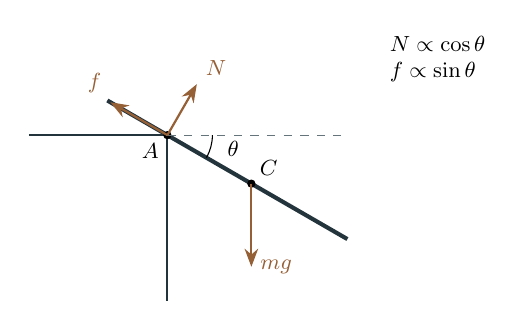
\begin{tikzpicture}[scale=.88,transform shape]
\draw[object](-2,0)--(0,0)--(0,-2.4);
\draw[object,line width=1.5pt](-0.8660254037844387,0.49999999999999994)--(2.598076211353316,-1.4999999999999998);
\fill(0,0)circle(1.7pt)node[below left]{$A$};
\fill(1.2124355652982142,-0.6999999999999998)circle(1.7pt)node[above right]{$C$};
\draw[guide](0,0)--(2.5,0);\draw(.65,0)arc(0:-30:.65);
\node at(.95,-.2){$\theta$};\draw[force](0,0)--(-0.8227241335952168,0.4749999999999999)node[above left]{$f$};
\draw[force](0,0)--(0.42499999999999993,0.7361215932167728)node[above right]{$N$};
\draw[force](1.2124355652982142,-0.6999999999999998)--(1.2124355652982142,-1.9)node[right]{$mg$};\node[align=left]at(3.9,1.1){$N\propto\cos\theta$\\$f\propto\sin\theta$};
\end{tikzpicture}
\figcaption{变图6.3V3\quad 沿杆与垂杆投影分别给摩擦和支持力}
\end{minipage}\end{center}
变图6.3V3中，先由绕角转动得 $\beta=mgb\cos\theta/(I_C+mb^2)$，再由初态积分得 $\omega^2=2mgb\sin\theta/(I_C+mb^2)$。代回两个质心投影方程，
\[N=\frac{mgI_C\cos\theta}{I_C+mb^2},\qquad f=\frac{mg(I_C+3mb^2)\sin\theta}{I_C+mb^2}.\]
取 $f\leq\mu N$ 的角度作为不滑动区间。
\item 薄板绕直边转动。
\begin{center}\begin{minipage}{.98\linewidth}\centering
\begin{tikzpicture}[scale=.88,transform shape]
\draw[object,fill=accent!8](-1,.58)--(2.6,-1.5)--(3.3,-.45)--(-.3,1.63)--cycle;
\draw[object](-2,0)--(0,0)--(0,-1.9);\draw[guide](0,0)--(1.3,-.75);\fill(1.3,-.75)circle(1.7pt)node[right]{$C$};
\draw[force](0,0)--(-.7,.404)node[left]{$f$};\draw[force](0,0)--(.45,.779)node[above]{$N$};
\node[below left]at(0,0){接触直边};
\end{tikzpicture}
\figcaption{变图6.3V4\quad 薄板绕直边转下，转动惯量取与边平行的质心轴}
\end{minipage}\end{center}
变图6.3V4中接触直边固定，质心到边的距离是 $b$。将绕平行于边的质心轴惯量记为 $I_C$，平行轴定理给 $I_A=I_C+mb^2$。重力矩、质心圆周运动的两投影保持相同形式，故 $f/N=(I_C+3mb^2)\tan\theta/I_C$，临界为 $\tan\theta_C=\mu I_C/(I_C+3mb^2)$。
\item 画出摩擦需求随角度的变化。
\begin{center}\begin{minipage}{.98\linewidth}\centering
\begin{tikzpicture}[scale=.88,transform shape]
\begin{scope}[x=4cm,y=1cm]
\draw[axis](0,0)--(1.15,0)node[right]{$\theta/\mathrm{rad}$};\draw[axis](0,0)--(0,3.6)node[above]{$f/N$};
\draw[traj,domain=0:1,samples=75]plot(\x,{2*tan(deg(\x))});\draw[guide](0,1.2)--(1.05,1.2)node[right]{$\mu$};
\draw[guide]({atan(.6)*pi/180},0)--({atan(.6)*pi/180},1.2);\node[below]at({atan(.6)*pi/180},0){$\theta_C$};\end{scope}
\end{tikzpicture}
\figcaption{变图6.3V5\quad 摩擦需求曲线与静摩擦系数相交}
\end{minipage}\end{center}
令 $K=1+3mb^2/I_C>1$。变图6.3V5以 $K=2,\mu=1.2$ 举例，曲线 $f/N=K\tan\theta$ 与水平线上下次序在交点处改变。因为导数 $K\sec^2\theta>0$，交点唯一，且在 $\pi/2$ 前有 $N>0$。
\item 水平初态已有转下角速度 $\omega_0$。
\begin{center}\begin{minipage}{.98\linewidth}\centering
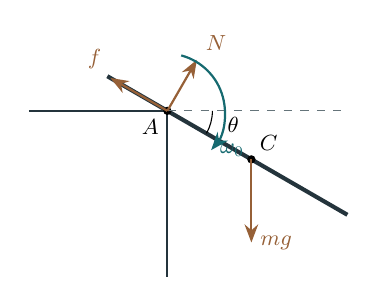
\begin{tikzpicture}[scale=.88,transform shape]
\draw[object](-2,0)--(0,0)--(0,-2.4);
\draw[object,line width=1.5pt](-0.8660254037844387,0.49999999999999994)--(2.598076211353316,-1.4999999999999998);
\fill(0,0)circle(1.7pt)node[below left]{$A$};
\fill(1.2124355652982142,-0.6999999999999998)circle(1.7pt)node[above right]{$C$};
\draw[guide](0,0)--(2.5,0);\draw(.65,0)arc(0:-30:.65);
\node at(.95,-.2){$\theta$};\draw[force](0,0)--(-0.8227241335952168,0.4749999999999999)node[above left]{$f$};
\draw[force](0,0)--(0.42499999999999993,0.7361215932167728)node[above right]{$N$};
\draw[force](1.2124355652982142,-0.6999999999999998)--(1.2124355652982142,-1.9)node[right]{$mg$};\draw[motion](.2,.8)arc(75:-40:.85)node[right]{$\omega_0$};
\end{tikzpicture}
\figcaption{变图6.3V6\quad 初始角速度额外增加向心加速度需求}
\end{minipage}\end{center}
变图6.3V6中初动能为 $I_A\omega_0^2/2$。由能量得
\[\omega^2=\omega_0^2+\frac{2mgb}{I_A}\sin\theta,\quad f=\frac{mg(I_C+3mb^2)}{I_A}\sin\theta+mb\omega_0^2.\]
支持力仍为 $mgI_C\cos\theta/I_A$。释放瞬间所需摩擦为 $mb\omega_0^2$，故先取 $mb\omega_0^2\leq\mu mgI_C/I_A$，再求 $f=\mu N$ 的首次交点。
\item 改为非均匀杆。
\begin{center}\begin{minipage}{.98\linewidth}\centering
\begin{tikzpicture}[scale=.88,transform shape]
\draw[object](-2,0)--(0,0)--(0,-2.4);
\draw[object,line width=1.5pt](-0.8660254037844387,0.49999999999999994)--(2.598076211353316,-1.4999999999999998);
\fill(0,0)circle(1.7pt)node[below left]{$A$};
\fill(0.692820323027551,-0.39999999999999997)circle(1.7pt)node[above right]{$C$};
\draw[guide](0,0)--(2.5,0);\draw(.65,0)arc(0:-30:.65);
\node at(.95,-.2){$\theta$};\draw[force](0,0)--(-0.8227241335952168,0.4749999999999999)node[above left]{$f$};
\draw[force](0,0)--(0.42499999999999993,0.7361215932167728)node[above right]{$N$};
\draw[force](0.692820323027551,-0.39999999999999997)--(0.692820323027551,-1.5999999999999999)node[right]{$mg$};\draw[object,line width=3pt](-.866,.5)--(.3,-.173);\node[above]at(-1.2,1.15){较密段};
\end{tikzpicture}
\figcaption{变图6.3V7\quad 非均匀杆先确定实际质心与质心惯量}
\end{minipage}\end{center}
变图6.3V7示意一端较密，先由 $x_C=\int x\dd m/m$ 求质心，再以该点算 $I_C=\int(x-x_C)^2\dd m$。用实际 $b=x_C-x_A$ 代入前面的通式。重力矩和向心需求使用同一个实际质心，杆长通过密度分布进入 $b,I_C$。
\item 比较摩擦、外伸与惯量对临界倾角的影响。
\begin{center}\begin{minipage}{.98\linewidth}\centering
\begin{tikzpicture}[scale=.88,transform shape]
\begin{scope}[x=4.8cm,y=.8cm]
\draw[axis](0,0)--(1.07,0)node[right]{$\theta/\mathrm{rad}$};\draw[axis](0,0)--(0,4.6)node[above]{$f/N$};
\draw[traj,domain=0:1,samples=65]plot(\x,{1.4*tan(deg(\x))});\draw[force,-,domain=0:1,samples=65]plot(\x,{2.6*tan(deg(\x))});
\draw[guide](0,1.5)--(1,1.5)node[right]{$\mu$};\node[above]at(.87,2.97){$mb^2/I_C$ 较大};\node[below]at(.85,1.49){$mb^2/I_C$ 较小};\end{scope}
\end{tikzpicture}
\figcaption{变图6.3V8\quad 外伸与惯量通过同一比值改变摩擦需求}
\end{minipage}\end{center}
变图6.3V8的纵坐标为 $f/N=(1+3mb^2/I_C)\tan\theta$。提高水平线 $\mu$，交点右移；在固定 $m,I_C$ 时增大 $b$，曲线上移，交点左移；在固定 $m,b$ 时增大 $I_C$，曲线下降，交点右移。这些变化来自向心需求与支持力的共同改变。
\end{enumerate}

\clearpage

\pdfbookmark[2]{第 4 题 实心圆柱体绕桌边下滚与开始滑动}{q4}

\section*{第 4 题\quad 实心圆柱体绕桌边下滚与开始滑动}

\tagline{M-06-04}

如图6.4,实心圆柱体从桌边由静止下滚,圆柱体与桌边之间的摩擦系数为\(\mu\).圆

柱体下滚过程中所转过的角度用 \(\theta\) 表示(如图6.4
所示).试求圆柱体开始相对桌边滑动时相应角度 \(\theta\)
所满足的关系式,并用图解法在图上标出这个角度以及不滑动的转角范围.

初态从静止作无穷小偏离后开始运动。

\begin{center}\begin{minipage}{\linewidth}\centering
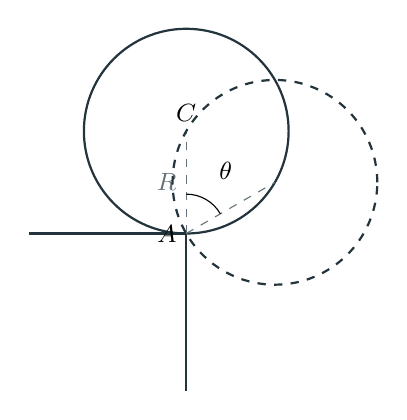
\begin{tikzpicture}[font=\small]
\draw[object](-2,0)--(0,0)--(0,-2);\draw[object](0,1.3)circle(1.3);\draw[guide](0,0)--(0,1.3)node[midway,left]{$R$};\node[left]at(0,0){$A$};\node[above]at(0,1.3){$C$};\draw[guide](0,0)--(1.125833025,.65);\draw[object,dashed](1.125833025,.65)circle(1.3);\draw(0,.5)arc(90:30:.5);\node at(.5,.8){$\theta$};
\end{tikzpicture}
\figcaption{图 6.4\quad 圆心绕固定桌角向右下方移动。}
\end{minipage}\end{center}

\Needspace{5\baselineskip}

\pdfbookmark[3]{题型定位}{q4-h0}

\subsection*{题型定位}

圆柱绕桌角下滚的摩擦临界与接触条件。

\Needspace{5\baselineskip}

\pdfbookmark[3]{知识点}{q4-h1}

\subsection*{知识点}

绕桌角的圆周运动、纯滚约束、能量积分、所需静摩擦与支持力。静摩擦达到上限时纯滚结束，支持力降为零时接触结束；本题有限正摩擦下前一种状态先到达。


\Needspace{5\baselineskip}

\pdfbookmark[3]{物理图像}{q4-h2}

\subsection*{物理图像}

圆柱从桌边绕接触点下滚，若无滑，圆柱相当于绕桌边瞬时固定点转动。重力矩让角速度增加，接触点同时需要支持力和摩擦维持滚动约束。

解图6.4A中圆心轨道半径是 $R$，支持力沿 $AC$ 朝外，摩擦沿切线阻碍下滚。

\Needspace{5\baselineskip}

\pdfbookmark[3]{解题入口}{q4-h3}

\subsection*{解题入口}

先以未滑动阶段的 $I_A=I_C+mR^2$ 求转动加速度，积分得到角速度平方。支持力由径向方程给出，摩擦由切向方程给出。把 $f$ 与 $\mu N$ 乘以同一因子后画在同一坐标系，交点给出起滑角。

\Needspace{5\baselineskip}

\pdfbookmark[3]{标准解法}{q4-h4}

\subsection*{标准解法}

\begin{center}\begin{minipage}{\linewidth}\centering
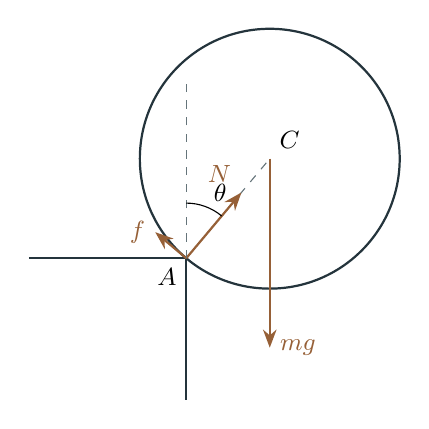
\begin{tikzpicture}[font=\small]
\draw[object](-2,0)--(0,0)--(0,-1.8);
\coordinate(C)at(1.060599556,1.263973331);\draw[object](C)circle(1.65);
\draw[guide](0,0)--(C);
\draw[force](0,0)--(.700541357,.834872679)node[above left]{$N$};
\draw[force](0,0)--(-.393923101,.330540729)node[left]{$f$};
\draw[force](C)--++(0,-2.4)node[right]{$mg$};
\draw[guide](0,0)--(0,2.3);\draw(0,.7)arc(90:50:.7);
\node at(.43,.83){$\theta$};\node[above right]at(C){$C$};
\node[below left]at(0,0){$A$};
\end{tikzpicture}
\figcaption{解图 6.4A\quad 支持力沿桌角至圆心，摩擦沿接触切线；角度从竖直向上量起。}
\end{minipage}\end{center}
解图6.4A中 $\theta$ 是 $AC$ 相对初始竖直方向的转角。不滑动阶段圆柱绕桌角 $A$ 转动，$I_A=I_C+mR^2=3mR^2/2$。径向、切向及绕 $A$ 的方程为
\[
 mg\cos\theta-N=mR\dot\theta^2,\quad
 mg\sin\theta-f=mR\ddot\theta,\quad
 mgR\sin\theta=I_A\ddot\theta.
\]
故 $\ddot\theta=2g\sin\theta/(3R)$、$f=mg\sin\theta/3$。利用 $\ddot\theta=\dot\theta\,\dd\dot\theta/\dd\theta$，积分得到
\[
 \frac12\dot\theta^2=-\frac{2g}{3R}\cos\theta+C_0,
 \quad C_0=\frac{2g}{3R},\quad
 \dot\theta^2=\frac{4g}{3R}(1-\cos\theta).
\]
能量法保留同样的初态与约束：$mgR(1-\cos\theta)=I_A\dot\theta^2/2$，也给出上式。代回径向方程：
\[
 N=mg\left[\cos\theta-\frac43(1-\cos\theta)\right]
 =\frac{mg}{3}(7\cos\theta-4).
\]
不滑动要求 $N\ge0$ 且 $f\le\mu N$，临界角满足
\[\result{\sin\theta_C=\mu(7\cos\theta_C-4).}\]
\begin{center}\begin{minipage}{\linewidth}\centering
\begin{tikzpicture}[font=\small,x=4.4cm,y=2.8cm]
\fill[accent!7](0,0)rectangle(.584295501,1.05);
\draw[axis](0,0)--(1.1,0)node[right]{$\theta/\mathrm{rad}$};
\draw[axis](0,0)--(0,1.25)node[above]{$y$};
\draw[traj,domain=0:.584295501,samples=70]plot(\x,{sin(deg(\x))});
\draw[thick,color=warm,domain=0:.584295501,samples=70]plot(\x,{.3*(7*cos(deg(\x))-4)});
\draw[traj,dashed,domain=.584295501:.962550748,samples=60]plot(\x,{sin(deg(\x))});
\draw[thick,color=warm,dashed,domain=.584295501:.962550748,samples=60]plot(\x,{.3*(7*cos(deg(\x))-4)});
\draw[guide](.584295501,0)--(.584295501,.551611896);
\fill(.584295501,.551611896)circle(.8pt);
\node[below]at(.584295501,0){$\theta_C$};
\node[below]at(.962550748,0){$\theta_0$};
\node[left]at(0,.9){$3\mu$};
\node[above]at(.8,.85){$\sin\theta$};
\draw[guide](.25,.834716)--(.36,1.06);
\node[above]at(.39,1.06){$\mu(7\cos\theta-4)$};
\draw[line width=2pt,accent](0,-.27)--(.584295501,-.27)node[midway,below]{不滑};
\end{tikzpicture}
\figcaption{解图 6.4B\quad 取$\mu=0.3$，交点与零点按计算定位；交点后的虚线只延拓纯滚表达式。}
\end{minipage}\end{center}
解图6.4B画的是无量纲的 $3f/(mg)=\sin\theta$ 与 $3\mu N/(mg)=\mu(7\cos\theta-4)$，交点给 $\theta_C$。前者递增，后者递减，在 $0\le\theta\le\arccos(4/7)$ 内只有一交点。不滑范围为 $0\le\theta\le\theta_C$。

若要在解图6.4B中准确定位交点，可令$z=\tan(\theta_C/2)$。
临界方程变为
\[
2z=\mu(3-11z^2),\qquad
z=\frac{\sqrt{1+33\mu^2}-1}{11\mu}
=\frac{3\mu}{1+\sqrt{1+33\mu^2}},
\]
\[
\theta_C=2\arctan\frac{3\mu}{1+\sqrt{1+33\mu^2}}\quad(\mu>0).
\]
只取正根；另一根对应负角，不属于由顶端向右下滚的过程。
图示$\mu=0.3$时，$\theta_C$约为$33.5^\circ$。
小$\mu$时$\theta_C\simeq3\mu$（弧度）；$\mu$增大时它趋近
$\arccos(4/7)$但始终小于该角，和图中滑动先于纯滚延拓的零压力点相符。

对有限正 $\mu$，$7\cos\theta_C-4=\sin\theta_C/\mu>0$，因此滑动先于脱离。图中 $\theta_0=\arccos(4/7)$ 是纯滚表达式的零支持力角。实际圆柱先在 $\theta_C$ 滑动，随后由滑动方程求支持力降到零的位置。严格位于顶端且完全静止是非稳定平衡，本题下滚理解为无穷小扰动后的过程。
\subsubsection*{积分步骤与曲线有效区间}
由转动方程消去$I_A$得到$\ddot\theta=2g\sin\theta/(3R)$。
这里对角速度使用链式法则，导数的分母应为角度：
\[
\ddot\theta=\frac{\dd\dot\theta}{\dd t}
=\frac{\dd\dot\theta}{\dd\theta}\frac{\dd\theta}{\dd t}
=\dot\theta\frac{\dd\dot\theta}{\dd\theta}.
\]
所以积分的两端可直接写为
\[
\int_0^{\dot\theta}u\dd u
=\frac{2g}{3R}\int_0^\theta\sin v\dd v
=\frac{2g}{3R}(1-\cos\theta).
\]
若用不定积分，初值$\theta=0,\dot\theta=0$给
$0=-2g/(3R)+C_0$，即$C_0=2g/(3R)$。
无滑接触点$A$的速度为零，支持力和静摩擦均不对圆柱做功；
因此能量式中的动能既可写成$I_A\dot\theta^2/2$，
也可分成质心平动与自转两项：
\[
\frac12mR^2\dot\theta^2+\frac12I_C\dot\theta^2
=\frac34mR^2\dot\theta^2.
\]
两种写法都包含质心平动与圆柱自转，纯滚时它们的速度通过同一个角速度联系起来。

解图6.4B的上升曲线表示所需摩擦，下弯曲线表示可供上限，
纵坐标分别乘同一个$3/(mg)$，才可以直接比较。
在压力为正的纯滚区间中，令$q= f/N$，有
\[
q(\theta)=\frac{\sin\theta}{7\cos\theta-4},
\qquad
q'(\theta)=\frac{7-4\cos\theta}{(7\cos\theta-4)^2}>0.
\]
从顶点的$q=0$到$\theta_0=\arccos(4/7)$前的$q\to+\infty$，
任何有限正$\mu$都只有一个交点。
因此实线区间$0\leq\theta\leq\theta_C$满足无滑条件；
交点之后的虚线延续纯滚表达式，实际受力从交点起按动摩擦和独立的自转速度计算。
图示$\mu=0.3$时，计算给
\[
\theta_C=0.5842955010\,\mathrm{rad}=33.4776662^\circ,
\qquad
\theta_0=0.9625507479\,\mathrm{rad}=55.1500954^\circ.
\]
在临界处$N_C=mg\sin\theta_C/(3\mu)>0$，
所以应先换成滑动方程；“先滑动”与“已经离边”对应不同的接触状态。
当$\mu\to0^+$时临界角趋零；当$\mu\to\infty$时，
$\theta_0-\theta_C\sim1/(7\mu)$，
有限摩擦的交点始终在零压力延拓角之前。

严格位于最高点并完全静止时，重力矩为零，数学解会一直停在顶点。
可先从一个任意小的正角$\theta_i$静止释放，得到
\[
\dot\theta^2=\frac{4g}{3R}(\cos\theta_i-\cos\theta),
\qquad
N=\frac{mg}{3}(7\cos\theta-4\cos\theta_i),
\]
再取$\theta_i\to0^+$恢复本题关系。
这个有限初角模型也须先满足$\tan\theta_i\leq3\mu$，
若这一条件不满足，释放瞬间即开始滑动。


\Needspace{5\baselineskip}

\pdfbookmark[3]{关键洞察}{q4-h5}

\subsection*{关键洞察}

在起滑处 $N_C=mg\sin\theta_C/(3\mu)>0$，圆柱仍接触桌角。解图6.4B中，$\theta_C$ 右侧两条虚线说明维持纯滚所需的摩擦已超过上限；实际圆柱此后沿桌角滑动，直到支持力为零。

\Needspace{5\baselineskip}

\pdfbookmark[3]{易错点}{q4-h6}

\subsection*{易错点}

无滑时质心轨道的速度和自转角速度满足 $v_C=R\dot\theta$。滑动后两种速度分别由质心方程与自转方程求出。摩擦图采用 $3f/(mg)$ 与 $3\mu N/(mg)$，两者的交点对应 $f=\mu N$。

\Needspace{5\baselineskip}

\pdfbookmark[3]{课堂讲解建议}{q4-h7}

\subsection*{课堂讲解建议}

在解图6.4B上问：“哪条线是维持纯滚所需的摩擦，哪条线是接触能提供的上限？”让学生沿两线走到交点，再用 $N_C>0$ 说明这时仍接触。最后从一个小正角 $\theta_i$ 静止释放，写出初始 $f/N=\tan\theta_i/3$，说明怎样选择能从纯滚开始的初态。


\Needspace{5\baselineskip}

\pdfbookmark[3]{变式训练}{q4-h8}

\subsection*{变式训练}

\begin{enumerate}
\item 改变 $\mu$。
\begin{center}\begin{minipage}{.98\linewidth}\centering
\begin{tikzpicture}[scale=.88,transform shape]
\begin{scope}[x=5cm,y=.8cm]
\draw[axis](0,0)--(1.08,0)node[right]{$\theta/\mathrm{rad}$};\draw[axis](0,0)--(0,4.2)node[above]{$f/N$};
\draw[traj,domain=0:.919,samples=80]plot(\x,{sin(deg(\x))/(7*cos(deg(\x))-4)});
\draw[guide](0,.3)--(.99,.3)node[right]{$\mu_1$};\draw[guide](0,1)--(.99,1)node[right]{$\mu_2$};
\draw[guide](.96255,0)--(.96255,4);\node[below]at(.96255,0){$\theta_0$};\end{scope}
\end{tikzpicture}
\figcaption{变图6.4V1\quad 摩擦系数增大时，临界交点沿曲线右移}
\end{minipage}\end{center}
变图6.4V1中 $q=\sin\theta/(7\cos\theta-4)$，导数为 $(7-4\cos\theta)/(7\cos\theta-4)^2>0$。把水平线从 $\mu_1$ 升到 $\mu_2$，唯一交点右移，临界角增加。对有限正摩擦，交点在分母为零的 $\theta_0$ 前。
\item 薄壁圆筒。
\begin{center}\begin{minipage}{.98\linewidth}\centering
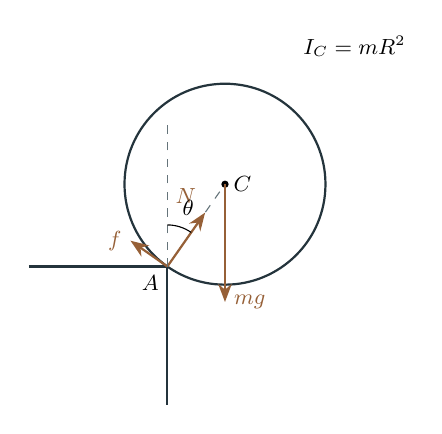
\begin{tikzpicture}[scale=.88,transform shape]
\draw[object](-2,0)--(0,0)--(0,-2);
\coordinate(C)at(0.8316858327090167,1.187770464219038);\draw[object](C)circle(1.45);
\draw[guide](0,0)--(C);\fill(C)circle(1.5pt)node[right]{$C$};
\node[below left]at(0,0){$A$};
\draw[force](0,0)--(0.5448976145334937,0.7781944420745421)node[above left]{$N$};
\draw[force](0,0)--(-0.5324488287878447,0.37282468362817994)node[left]{$f$};
\draw[force](C)--++(0,-1.7)node[right]{$mg$};
\draw[guide](0,0)--(0,2.1);\draw(0,.6)arc(90:55:.6);
\node at(.3,.85){$\theta$};\node[above]at(2.7,2.9){$I_C=mR^2$};
\end{tikzpicture}
\figcaption{变图6.4V2\quad 薄壁圆筒保留相同几何，转动惯量改变}
\end{minipage}\end{center}
变图6.4V2取 $I_A=2mR^2$，重力矩给 $\ddot\theta=g\sin\theta/(2R)$，从顶端小扰动的能量积分给 $\dot\theta^2=g(1-\cos\theta)/R$。切向与径向方程分别得到
\[f=\tfrac12mg\sin\theta,\qquad N=mg(2\cos\theta-1).\]
因此临界式为 $\sin\theta=2\mu(2\cos\theta-1)$。
\item 纯滚压力零点与实际离边。
\begin{center}\begin{minipage}{.98\linewidth}\centering
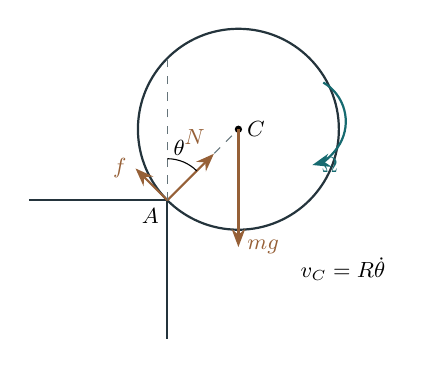
\begin{tikzpicture}[scale=.88,transform shape]
\draw[object](-2,0)--(0,0)--(0,-2);
\coordinate(C)at(45:1.45);\draw[object](C)circle(1.45);
\draw[guide](0,0)--(C);\fill(C)circle(1.5pt)node[right]{$C$};
\node[below left]at(0,0){$A$};
\draw[force](0,0)--(45:.95)node[above left]{$N$};
\draw[force](0,0)--(135:.65)node[left]{$f$};
\draw[force](C)--++(0,-1.7)node[right]{$mg$};
\draw[guide](0,0)--(0,2.1);\draw(0,.6)arc(90:45:.6);
\node at(.17,.76){$\theta$};\draw[motion](2.25,1.7)arc(60:-75:.65)node[right]{$\Omega$};\node[below right]at(1.8,-.7){$v_C=R\dot\theta$};
\end{tikzpicture}
\figcaption{变图6.4V3\quad 滑动阶段质心绕角速度与自转角速度分别求解}
\end{minipage}\end{center}
实心柱纯滚式中的 $N=0$ 给 $\theta_0=\arccos(4/7)$。变图6.4V3在滑动阶段另标自转角速度 $\Omega$。令切向滑速为 $u=R(\dot\theta-\Omega)$、$s=\operatorname{sgn}u$，若动摩擦系数给定为 $\mu_k$，则
\[N=mg\cos\theta-mR\dot\theta^2,\quad mR\ddot\theta=mg\sin\theta-s\mu_kN,\quad I_C\dot\Omega=s\mu_kNR.\]
设实心柱的 $0\leq\mu_k\leq\mu$，从起滑点 $\theta_C>0$ 接续。取朝下滚方向的滑速为正，令 $s=1$，则
\[
\dot u=g\sin\theta-\frac{3\mu_kN}{m}.
\]
在起滑点 $\mu N_C=mg\sin\theta_C/3$，故 $\dot u(\theta_C)\geq0$，同时 $\ddot\theta\geq2g\sin\theta_C/(3R)>0$。继续下滚时，$\sin\theta$ 增大，$N=mg\cos\theta-mR\dot\theta^2$ 减小，因而下滚加速度和 $\dot u$ 都持续增大，直到离边。令 $W=\dot\theta^2$，得到
\[
\begin{aligned}
\frac{\dd W}{\dd\theta}-2\mu_k W&=\frac{2g}{R}(\sin\theta-\mu_k\cos\theta),\\
W(\theta)&=e^{2\mu_k(\theta-\theta_C)}
\left[W_C+\frac{2g}{R}\int_{\theta_C}^{\theta}
e^{-2\mu_k(\xi-\theta_C)}(\sin\xi-\mu_k\cos\xi)\dd\xi\right].
\end{aligned}
\]
用纯滚式给初值 $W_C$，首次满足 $W(\theta_d)=g\cos\theta_d/R$ 的角度就是实际离边角。变图6.4V3 取 $\mu=0.3,\ \mu_k=0.2$，起滑角约 $33.48^\circ$，离边角约 $52.01^\circ$，图中的 $45^\circ$ 仍处于滑动接触阶段。
\item 取 $\mu=0.3$，求临界角。
\begin{center}\begin{minipage}{.98\linewidth}\centering
\begin{tikzpicture}[scale=.88,transform shape]
\begin{scope}[x=5.2cm,y=2.3cm]
\draw[axis](0,0)--(1.07,0)node[right]{$\theta/\mathrm{rad}$};\draw[axis](0,-1)--(0,1.2)node[above]{$F(\theta)$};
\draw[traj,domain=0:.962550748,samples=80]plot(\x,{sin(deg(\x))-.3*(7*cos(deg(\x))-4)});
\fill(.584295501,0)circle(1.8pt);\draw[guide](.584295501,-.7)--(.584295501,.55);\node[below]at(.584295501,-.7){$0.5843$};\end{scope}
\end{tikzpicture}
\figcaption{变图6.4V4\quad 临界函数从负值增至正值，只有一个零点}
\end{minipage}\end{center}
令 $F(\theta)=\sin\theta-0.3(7\cos\theta-4)$。变图6.4V4中 $F(0)=-0.9$，$F(\theta_0)=\sin\theta_0>0$，且 $F'=\cos\theta+2.1\sin\theta>0$。二分每次保留异号的半区间，得到
\[\theta_C=0.5842955010\ \mathrm{rad}=33.4776662^\circ.\]
此处 $N/(mg)=\sin\theta_C/0.9>0$。
\item 比较圆柱与细杆的启动与摩擦需求。
\begin{center}\begin{minipage}{.98\linewidth}\centering
\begin{tikzpicture}[scale=.88,transform shape]
\draw[axis](0,0)--(5.6,0)node[right]{$\theta$};\draw[axis](0,0)--(0,3)node[above]{摩擦需求};
\draw[traj](0,0)..controls(2,.2)and(3,1.6)..(3.9,2.7)node[right]{细杆：$K\tan\theta$};
\draw[force,-](0,0)..controls(1.9,.1)and(2.5,.2)..(2.9,2.7)node[above]{圆柱};
\draw[guide](3,0)--(3,2.6);\node[below]at(3,0){$\arccos(4/7)$};\node[below]at(5,0){$\pi/2$};
\end{tikzpicture}
\figcaption{变图6.4V5\quad 示意两类需求曲线的发散角，纵向高度用于比较形状}
\end{minipage}\end{center}
变图6.4V5示意两种曲线。细杆外伸 $b>0$ 时，初始重力矩 $mgb$ 非零，$f/N=K\tan\theta$ 在 $\pi/2$ 前持续增加。圆柱处于顶端时重力矩为零，需小偏离启动；它的 $f/N$ 在较早的 $\arccos(4/7)$ 前发散。两者的有限正摩擦交点均先于各自支持力为零的纯滚角。
\item 从 $\theta_i>0$ 静止释放。
\begin{center}\begin{minipage}{.98\linewidth}\centering
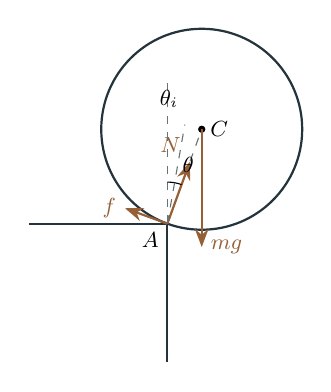
\begin{tikzpicture}[scale=.88,transform shape]
\draw[object](-2,0)--(0,0)--(0,-2);
\coordinate(C)at(0.4959292078222196,1.3625543001395672);\draw[object](C)circle(1.45);
\draw[guide](0,0)--(C);\fill(C)circle(1.5pt)node[right]{$C$};
\node[below left]at(0,0){$A$};
\draw[force](0,0)--(0.3249191361593853,0.8927079897466129)node[above left]{$N$};
\draw[force](0,0)--(-0.6108002035108405,0.22231309316168468)node[left]{$f$};
\draw[force](C)--++(0,-1.7)node[right]{$mg$};
\draw[guide](0,0)--(0,2.1);\draw(0,.6)arc(90:70:.6);
\node at(.3,.85){$\theta$};\draw[guide](0,0)--(.2517899,1.427971);\node[above left]at(.28,1.55){$\theta_i$};
\end{tikzpicture}
\figcaption{变图6.4V6\quad 从有限小正角静止释放}
\end{minipage}\end{center}
变图6.4V6中从初始到当前位置的势能减少为 $mgR(\cos\theta_i-\cos\theta)$，于是
\[\dot\theta^2=\frac{4g}{3R}(\cos\theta_i-\cos\theta),\quad N=\frac{mg}{3}(7\cos\theta-4\cos\theta_i).\]
摩擦仍为 $mg\sin\theta/3$。初态 $f/N=\tan\theta_i/3$，取 $\tan\theta_i\leq3\mu$ 才从无滑开始；随后解 $\sin\theta=\mu(7\cos\theta-4\cos\theta_i)$ 的首次交点。
\item 一般转动惯量 $I_C=kmR^2$。
\begin{center}\begin{minipage}{.98\linewidth}\centering
\begin{tikzpicture}[scale=.88,transform shape]
\begin{scope}[x=.9cm,y=4cm]
\draw[axis](0,0)--(5.2,0)node[right]{$k$};\draw[axis](0,0)--(0,1.3)node[above]{$\theta_0/\mathrm{rad}$};
\draw[traj,domain=0:4.8,samples=80]plot(\x,{acos(2/(\x+3))*pi/180});
\draw[guide](.5,0)--(.5,{acos(4/7)*pi/180});\fill(.5,{acos(4/7)*pi/180})circle(1.5pt);\node[below]at(.5,0){$1/2$};\end{scope}
\end{tikzpicture}
\figcaption{变图6.4V7\quad 一般惯量下，纯滚压力零点随惯量比改变}
\end{minipage}\end{center}
变图6.4V7比较纯滚压力零点。以 $I_A=(1+k)mR^2$ 求得 $\ddot\theta=g\sin\theta/[(1+k)R]$、$\dot\theta^2=2g(1-\cos\theta)/[(1+k)R]$。因此
\[f=\frac{kmg\sin\theta}{1+k},\quad N=\frac{mg[(k+3)\cos\theta-2]}{1+k}.\]
临界式为 $k\sin\theta=\mu[(k+3)\cos\theta-2]$，纯滚压力零点为 $\theta_0=\arccos[2/(k+3)]$。
\item 画出下滚全过程的阶段。
\begin{center}\begin{minipage}{.98\linewidth}\centering
\begin{tikzpicture}[scale=.88,transform shape]
\draw[axis](0,0)--(10,0)node[right]{运动过程};
\foreach \x/\t in {0/小角释放,3/静摩擦达上限,6/沿桌角滑动,9/支持力为零}{\fill(\x,0)circle(1.7pt);\node[above,align=center]at(\x,.25){\t};}
\draw[traj,line width=2pt](0,-.6)--(3,-.6)node[midway,below]{$v_C=R\Omega$};
\draw[force,-,line width=2pt](3,-.6)--(9,-.6)node[midway,below]{质心运动与自转分别计算};
\end{tikzpicture}
\figcaption{变图6.4V8\quad 无滑关系只用于第一阶段}
\end{minipage}\end{center}
变图6.4V8从小角释放开始，第一段取静摩擦维持 $v_C=R\Omega$，直到 $f=\mu N$。接着用滑动阶段的质心和自转方程，保持位置、速度连续；支持力首次到零时，桌角接触结束，随后质心在重力下运动，圆柱绕质心继续自转。
\end{enumerate}

\clearpage

\pdfbookmark[2]{第 5 题 甲虫落到可转动麦杆后的运动}{q5}

\section*{第 5 题\quad 甲虫落到可转动麦杆后的运动}

\tagline{M-06-05}

如图,均匀细麦杆长\(l\),可绕通过中心\(O\)的固定水平轴在铅垂面内自由转动.开始时麦杆静止于水平位置.一质量与麦杆相同的甲虫以速度\(v_{0}\)垂直落到麦杆的\(\frac{1}{4}\)长度处,落下后立即向端点爬行.

试问:1. 为使麦杆以均匀的角速度转动,甲虫沿麦杆爬行的速度应是多少? 2.
甲虫轨迹的参变方程是什么? 3.
为了使甲虫在麦杆转到铅直位置前能爬到端点,甲虫下落速度 \(v_{0}\)
的最高值是多少?

\begin{center}\begin{minipage}{\linewidth}\centering
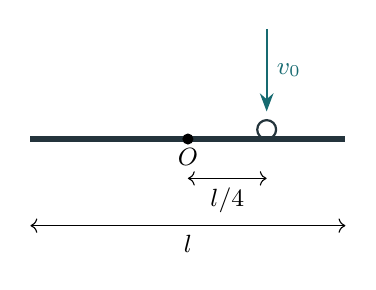
\begin{tikzpicture}[font=\small]
\draw[object,line width=2pt](-2,0)--(2,0);\fill(0,0)circle(2pt)node[below]{$O$};\draw[object](1,.12)circle(.12);\draw[motion](1,1.4)--(1,.35)node[midway,right]{$v_0$};\draw[<->](0,-.5)--(1,-.5)node[midway,below]{$l/4$};\draw[<->](-2,-1.1)--(2,-1.1)node[midway,below]{$l$};
\end{tikzpicture}
\figcaption{图 6.5\quad 甲虫落点离中心 $l/4$，随后沿杆向右端爬行。}
\end{minipage}\end{center}

\Needspace{5\baselineskip}

\pdfbookmark[3]{题型定位}{q5-h0}

\subsection*{题型定位}

甲虫落杆的碰撞角动量，以及主动爬行下的变惯量转动。

\Needspace{5\baselineskip}

\pdfbookmark[3]{知识点}{q5-h1}

\subsection*{知识点}

碰撞的轴角动量、随径向位置变化的惯量、重力矩、恒角速度与参数轨迹。碰撞先确定角速度，随后重力矩使角动量增加，甲虫以增加惯量的方式保持角速度。


\Needspace{5\baselineskip}

\pdfbookmark[3]{物理图像}{q5-h2}

\subsection*{物理图像}

甲虫落到水平麦杆上后随杆转动，并沿杆向外爬行。它到支轴的距离增大，系统惯量随之增加；恒角速度所需的惯量增长率由甲虫重力的轴力矩决定。

落杆捕获时，支轴冲量关于 $O$ 的力矩为零，以轴角动量连接碰前和碰后。随后主动爬行，解图6.5A中 $r$ 增大使惯量增大，重力矩持续提供维持同一角速度所需增加的角动量。

\Needspace{5\baselineskip}

\pdfbookmark[3]{解题入口}{q5-h3}

\subsection*{解题入口}

落杆时对支轴 $O$ 取角动量，再在爬行时写 $\dd(I\omega)/\dd t=mgr\cos\varphi$。取 $\dot\omega=0$ 后解出径向速度，积分常数由实际落点给出。最后把 $r=l/2$ 代入，比较到端角与 $\pi/2$。

\Needspace{5\baselineskip}

\pdfbookmark[3]{标准解法}{q5-h4}

\subsection*{标准解法}

\begin{center}\begin{minipage}{\linewidth}\centering
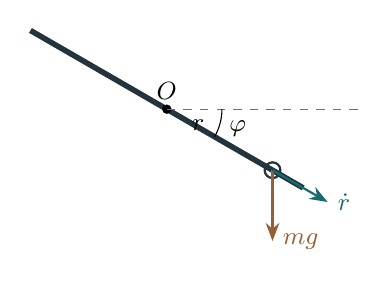
\begin{tikzpicture}[font=\small]
\draw[object,line width=2pt](-1.732050808,1)--(1.732050808,-1);
\fill(0,0)circle(1.7pt)node[above]{$O$};\coordinate(P)at(1.342339376,-.775);
\draw[object](P)circle(.1);\draw[force](P)--++(0,-.9)node[right]{$mg$};
\draw[motion](P)--++(.7,-.404145188)node[right]{$\dot r$};
\draw[guide](0,0)--(2.5,0);\draw(.7,0)arc(0:-30:.7);
\node at(.9,-.25){$\varphi$};\node[above left]at(.6,-.4){$r$};
\end{tikzpicture}
\figcaption{解图 6.5A\quad $r$ 为甲虫到支轴距离，$\dot r$ 为相对杆的径向爬速。}
\end{minipage}\end{center}
甲虫落点到杆中心的距离 $r_0=l/4$；杆与甲虫的质量均为 $m$。碰撞期间支轴冲量关于 $O$ 的矩为零，重力冲量矩可忽略。系统关于 $O$ 的角动量守恒：
\[
 mv_0\frac l4=\left(\frac1{12}ml^2+m\frac{l^2}{16}\right)\omega,
 \qquad\result{\omega=\frac{12v_0}{7l}.}
\]
碰后麦杆自身的重力通过 $O$，只有甲虫产生重力矩。解图6.5A以向下转角 $\varphi=\omega t$ 为正，$I(t)=ml^2/12+mr^2$。恒角速度要求
\[
 mgr\cos\varphi=\frac{\dd(I\omega)}{\dd t}
 =\omega(2mr\dot r),
 \qquad\result{\dot r=\frac g{2\omega}\cos(\omega t).}
\]
这是相对杆的爬行速度；甲虫在空间的速度还含切向分量 $r\omega$。积分时先保留上下限和初始位置：
\[
 \int_{l/4}^{r(t)}\dd r=\frac g{2\omega}\int_0^t\cos(\omega t')\dd t'
 =\frac g{2\omega^2}\sin(\omega t).
\]
积分起点取落点半径 $r(0)=l/4$，于是
\[
 r(t)=\frac l4+\frac g{2\omega^2}\sin(\omega t),\qquad
 \varphi(t)=\omega t.
\]
\Needspace{19\baselineskip}
\begin{center}\begin{minipage}{\linewidth}\centering
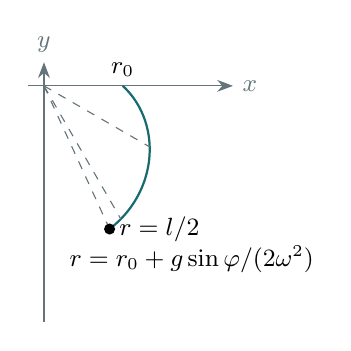
\begin{tikzpicture}[font=\small]
\draw[axis](-.2,0)--(2.4,0)node[right]{$x$};\draw[axis](0,-3)--(0,.3)node[above]{$y$};\draw[traj,domain=0:65.380022671,samples=70]plot({(1+1.1*sin(\x))*cos(\x)},{-(1+1.1*sin(\x))*sin(\x)});\foreach \t in {0,30,60,65.380022671}{\draw[guide](0,0)--({(1+1.1*sin(\t))*cos(\t)},{-(1+1.1*sin(\t))*sin(\t)});}\node[above]at(1,0){$r_0$};\fill(.833195581,-1.818181818)circle(2pt)node[right]{$r=l/2$};\node[right]at(.2,-2.2){$r=r_0+g\sin\varphi/(2\omega^2)$};
\end{tikzpicture}
\figcaption{解图 6.5B\quad 甲虫空间轨迹为极径随转角增长的曲线；在到端时截断。}
\end{minipage}\end{center}
解图6.5B按 $x=r\cos\varphi$、$y=-r\sin\varphi$ 将极坐标轨迹转成直角坐标。图中甲虫在杆转到铅直前到端，所以曲线在 $r=l/2$ 处结束。如果转到铅直仍未到端，匀速向外爬行这一段止于 $\varphi=\pi/2$，此时 $\dot r=0$。

杆转到铅直时 $t_v=\pi/(2\omega)$。甲虫要在此前或同时到端，需
\[
 \frac l4+\frac g{2\omega^2}\ge\frac l2
 \Longrightarrow \omega^2\le\frac{2g}{l}
 \Longrightarrow\result{v_0\le\frac7{\sqrt{72}}\sqrt{gl}.}
\]
若“之前”取严格含义，则改为严格小于；等号意味着恰在铅直时到端。到端后若甲虫留在杆端，惯量固定，随后的角速度由重力矩决定。
\subsubsection*{角动量变化、积分常量与到端时刻}
落杆瞬间的惯量可分项算清：
\[
I_0=\left(\frac1{12}+\frac1{16}\right)ml^2
=\frac7{48}ml^2,
\qquad
\omega=\frac{mv_0l/4}{7ml^2/48}=\frac{12v_0}{7l}.
\]
径向爬速不贡献关于$O$的角动量，因为径向速度与矢径平行。
但它会改变$r$及转动惯量；碰后系统的外力矩为$mgr\cos\varphi$，并不为零。
完整角动量方程展开为
\[
mgr\cos\varphi
=\left(\frac1{12}ml^2+mr^2\right)\dot\omega
+2mr\dot r\,\omega.
\]
只有代入题设$\dot\omega=0$以后，才得到所需爬速。
其中$r>0,\omega>0$；从$\varphi=0$转到$\pi/2$的过程中，
$\cos\varphi\geq0$，所以甲虫始终向外爬，爬速逐渐减小。
若甲虫不爬，第二项消失，重力矩便使角速度增大。

积分也可写成$r=g\sin(\omega t)/(2\omega^2)+C_0$。
将$t=0,r=l/4$同时代入得$C_0=l/4$，
再与$\varphi=\omega t$组成极坐标参变方程。
解图6.5B的坐标约定是右方为$x$正向、上方为$y$正向，
而$\varphi$向下为正，故
\[
x(t)=\left[\frac l4+\frac g{2\omega^2}\sin(\omega t)\right]\cos(\omega t),
\]
\[
y(t)=-\left[\frac l4+\frac g{2\omega^2}\sin(\omega t)\right]\sin(\omega t).
\]
这里$\dot r$与$r\omega$互相垂直，空间速率由这两个正交分量合成，为 $v=\sqrt{\dot r^2+r^2\omega^2}$。

到端条件可进一步求成时刻，令$\zeta=\omega^2l/(2g)$。
由$r(t_e)=l/2$得到
\[
\sin\varphi_e=\zeta,
\qquad \varphi_e=\arcsin\zeta,
\qquad t_e=\frac{\arcsin\zeta}{\omega}.
\]
因此 $0<\zeta\leq1$ 才会在 $0<\varphi\leq\pi/2$ 到端。当 $\zeta>1$，铅直时 $r=l/4+g/(2\omega^2)<l/2$，继续保持同一角速度将要求 $\dot r<0$。
$t_e\leq\pi/(2\omega)$恰与前面的$\omega^2\leq2g/l$相同。
等号给$\varphi_e=\pi/2$，严格小于给提前到端。
若“前”严格排除同时到达，$7\sqrt{gl/72}$是允许速度的上确界，
允许速度严格小于这个上确界。

解图6.5A、B采用同一示例$g/(2\omega^2)=1.1r_0$。
图中取$r_0$为长度单位，则$l/2=2$，
$30^\circ$时$r=1.55$，到端角为$\arcsin(1/1.1)=65.3800227^\circ$，
终点坐标为$(0.8331956,-1.8181818)$。
曲线和终点均由这些参数计算，到端时曲线截断。

\subsubsection*{碰撞与主动爬行的能量条件}
若先看甲虫被麦杆接住、尚未建立径向爬速的瞬间，
碰后的转动动能与碰前动能之比为
\[
\frac{K_+}{K_-}
=\frac{(mv_0r_0)^2/(2I_0)}{mv_0^2/2}
=\frac{mr_0^2}{I_0}=\frac37.
\]
这个捕获过程损失了碰前动能的$4/7$。
规定的爬行函数在$t=0^+$却要求$\dot r=g/(2\omega)$，
建立这部分径向速度需要甲虫主动作用；它不改变上述轴角动量，
建立径向速度所需的能量由甲虫的主动爬行动作提供。爬行阶段的运动由外重力矩与变化中的惯量联系起来。

若严格提前到端，甲虫停在$r=l/2$以后，
在 $\varphi<\pi/2$ 时外重力矩仍为正，惯量已经固定，角速度随之增加。
因此匀角速度公式与解图6.5B的轨迹均止于到端时刻；
恰在铅直时到端的情形可让这段匀速过程一直延续到铅直位置。


\Needspace{5\baselineskip}

\pdfbookmark[3]{关键洞察}{q5-h5}

\subsection*{关键洞察}

向外爬行时，惯量变化率为 $2mr\dot r$。恒定角速度下，$\omega\dot I$ 恰好等于虫重的轴力矩。径向速度与矢径平行，关于支轴的瞬时角动量来自切向速度 $r\omega$。

\Needspace{5\baselineskip}

\pdfbookmark[3]{易错点}{q5-h6}

\subsection*{易错点}

相对杆的径向爬速为 $\dot r$，空间速度还含 $r\omega$。积分半径从 $l/4$ 开始。达到杆端后，爬行函数在这里结束。严格提前到端对应严格不等号，铅直时到端对应等号。

\Needspace{5\baselineskip}

\pdfbookmark[3]{课堂讲解建议}{q5-h7}

\subsection*{课堂讲解建议}

让学生在解图6.5A中画径向与切向速度，问：“哪一项直接贡献关于 $O$ 的角动量？”回答为切向速度。再问径向爬行怎样改变惯量，用 $\dot I=2mr\dot r$ 写清。沿解图6.5B找到 $r=l/2$ 的终点，比较它与铅直方向，最后把严格提前和同时到达分别写成不等式。


\Needspace{5\baselineskip}

\pdfbookmark[3]{变式训练}{q5-h8}

\subsection*{变式训练}

\begin{enumerate}
\item 甲虫质量改为杆质量的一半。
\begin{center}\begin{minipage}{.98\linewidth}\centering
\begin{tikzpicture}[scale=.88,transform shape]
\draw[object,line width=1.6pt](-1.732,1)--(1.732,-1);
\fill(0,0)circle(1.7pt)node[above left]{$O$};
\filldraw[object,fill=white](1.2,-.69282)circle(.1)node[above right]{$m$};
\draw[force](1.2,-.69282)--(1.2,-1.89)node[right]{$mg$};
\draw[guide](0,0)--(2.3,0);\draw(.65,0)arc(0:-30:.65);
\node at(.85,-.24){$\varphi$};\draw[motion](1.2,-.69282)--(1.86,-1.07387)node[right]{$\dot r$};\node[above]at(-1.2,1.1){杆质量 $M$};\node[right]at(2,-1.3){虫质量 $M/2$};
\end{tikzpicture}
\figcaption{变图6.5V1\quad 质量改变后先重新计算捕获惯量}
\end{minipage}\end{center}
变图6.5V1取杆质量 $M$、虫质量 $m=M/2$，仍从 $r_0=l/4$ 落下。捕获角动量给 $\omega=mv_0r_0/(Ml^2/12+mr_0^2)=12v_0/(11l)$。爬行时 $mgr\cos\varphi=2mr\dot r\omega$，虫质量约去，得到 $\dot r=g\cos\varphi/(2\omega)$。
\item 任意落点 $r_0$。
\begin{center}\begin{minipage}{.98\linewidth}\centering
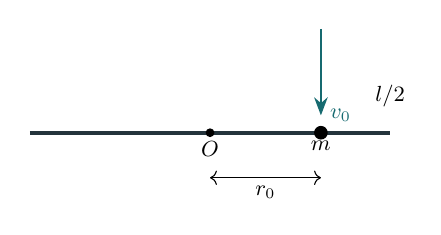
\begin{tikzpicture}[scale=.88,transform shape]
\draw[object,line width=1.6pt](-2.6,0)--(2.6,0);\fill(0,0)circle(1.8pt)node[below]{$O$};\fill(1.6,0)circle(2.8pt)node[below]{$m$};\draw[motion](1.6,1.5)--(1.6,.25)node[right]{$v_0$};\draw[<->](0,-.65)--(1.6,-.65)node[midway,below]{$r_0$};\node[above]at(2.6,.25){$l/2$};
\end{tikzpicture}
\figcaption{变图6.5V2\quad 任意落点提供的初始角动量与力臂成正比}
\end{minipage}\end{center}
变图6.5V2中，入射动量的力臂为 $r_0$，碰后惯量为 $I_0=Ml^2/12+mr_0^2$。因而 $\omega=mv_0r_0/I_0$。沿杆向外爬行取 $0<r_0<l/2$；落在中心时入射轴角动量为零。爬行半径为 $r=r_0+g\sin\varphi/(2\omega^2)$。
\item 甲虫停在落点不爬。
\begin{center}\begin{minipage}{.98\linewidth}\centering
\begin{tikzpicture}[scale=.88,transform shape]
\draw[object,line width=1.6pt](-1.732,1)--(1.732,-1);
\fill(0,0)circle(1.7pt)node[above left]{$O$};
\filldraw[object,fill=white](1.2,-.69282)circle(.1)node[above right]{$m$};
\draw[force](1.2,-.69282)--(1.2,-1.89)node[right]{$mg$};
\draw[guide](0,0)--(2.3,0);\draw(.65,0)arc(0:-30:.65);
\node at(.85,-.24){$\varphi$};\draw[guide](1.4,0)arc(0:-70:1.4);\node[above]at(1,1.1){$r=r_0$ 固定};
\end{tikzpicture}
\figcaption{变图6.5V3\quad 不爬时虫沿定半径圆弧运动}
\end{minipage}\end{center}
变图6.5V3中 $r=r_0$，总惯量 $I$ 固定。虫下降的势能转成转动动能，
\[\tfrac12 I(\omega^2-\omega_i^2)=mgr_0\sin\varphi,\quad \omega^2=\omega_i^2+2mgr_0\sin\varphi/I.\]
从水平到铅直，角速度逐渐增大。
\item 画出恒角速度爬行的空间轨迹。
\begin{center}\begin{minipage}{.98\linewidth}\centering
\begin{tikzpicture}[scale=.88,transform shape]
\begin{scope}[x=2.1cm,y=2.1cm]
\draw[axis](0,0)--(2.5,0)node[right]{$x/r_0$};\draw[axis](0,-2.3)--(0,.3)node[above]{$y/r_0$};
\draw[traj,domain=0:65.3800227,samples=80]plot({(1+1.1*sin(\x))*cos(\x)},{-(1+1.1*sin(\x))*sin(\x)});
\draw[guide](0,0)--(.83319558,-1.8181818);\fill(.83319558,-1.8181818)circle(1.7pt)node[right]{杆端};\end{scope}
\end{tikzpicture}
\figcaption{变图6.5V4\quad 半径随转角增大，曲线在杆端截断}
\end{minipage}\end{center}
变图6.5V4以 $r_0$ 为长度单位，取 $g/(2\omega^2)=1.1r_0$、$l/2=2r_0$。将极径投影到固定坐标，
\[x=[r_0+g\sin\varphi/(2\omega^2)]\cos\varphi,\quad y=-[r_0+g\sin\varphi/(2\omega^2)]\sin\varphi.\]
解 $r=l/2$ 得 $\varphi_e=\arcsin(1/1.1)$；曲线止于这个点。
\item 求捕获损失的动能。
\begin{center}\begin{minipage}{.98\linewidth}\centering
\begin{tikzpicture}[scale=.88,transform shape]
\begin{scope}[x=1cm,y=3cm]
\draw[axis](0,0)--(5.5,0);\draw[axis](0,0)--(0,1.25)node[above]{$K/K_i$};
\fill[accent!20](.7,0)rectangle(1.7,1);\fill[accent!45](3,0)rectangle(4,{3/7});\draw[guide](0,1)--(1.7,1)node[above]{$1$};\draw[guide](0,{3/7})--(4,{3/7})node[above]{$3/7$};\node[below]at(1.2,0){捕获前};\node[below]at(3.5,0){捕获后};\end{scope}
\end{tikzpicture}
\figcaption{变图6.5V5\quad 能量比较取尚未建立主动径向速度的捕获瞬间}
\end{minipage}\end{center}
变图6.5V5比较捕获前和刚捕获后。由 $L=mv_0r_0$，
\[K_i=mv_0^2/2,\quad K_f=L^2/(2I_0),\quad K_i-K_f=\tfrac12mv_0^2\left(1-\frac{mr_0^2}{I_0}\right).\]
本题 $mr_0^2/I_0=3/7$，损失比例为 $4/7$。随后的径向爬速由主动动作建立，它所需的动能在爬行阶段计算。
\item 改变到端的时间要求。
\begin{center}\begin{minipage}{.98\linewidth}\centering
\begin{tikzpicture}[scale=.88,transform shape]
\begin{scope}[x=.052cm,y=1.2cm]
\draw[axis](0,0)--(101,0)node[right]{$\varphi$};\draw[axis](0,0)--(0,2.8)node[above]{$r/r_0$};
\draw[traj,domain=0:65.3800227,samples=65]plot(\x,{1+1.1*sin(\x)});\draw[guide,domain=65.3800227:90,samples=40]plot(\x,{1+1.1*sin(\x)});
\draw[guide](0,2)--(90,2)node[right]{$l/(2r_0)$};\draw[guide](65.3800227,0)--(65.3800227,2);\node[below]at(65.3800227,0){$\varphi_e$};\node[below]at(90,0){$90^\circ$};\end{scope}
\end{tikzpicture}
\figcaption{变图6.5V6\quad 到端发生在半径曲线首次达到杆端水平线处}
\end{minipage}\end{center}
变图6.5V6中，半径曲线达到 $l/2$ 时结束。到端角满足 $\sin\varphi_e=2\omega^2(l/2-r_0)/g$。在 $\pi/2$ 以前或同时达到杆端，条件为
\[\frac g{2\omega^2}\geq l/2-r_0,\qquad \omega^2\leq\frac g{l-2r_0}.\]
严格提前取严格不等号。
\item 改变杆绕支轴的惯量。
\begin{center}\begin{minipage}{.98\linewidth}\centering
\begin{tikzpicture}[scale=.88,transform shape]
\begin{scope}[x=2.3cm,y=2.8cm]
\draw[axis](0,0)--(2.3,0)node[right]{$I_{\rm rod}/(mr_0^2)$};\draw[axis](0,0)--(0,1.2)node[above]{$\omega r_0/v_0$};
\draw[traj,domain=0:2.1,samples=65]plot(\x,{1/(1+\x)});\node[left]at(0,1){$1$};\end{scope}
\end{tikzpicture}
\figcaption{变图6.5V7\quad 杆惯量越大，同一捕获角动量分配给越大的总惯量}
\end{minipage}\end{center}
变图6.5V7中 $\omega r_0/v_0=1/[1+I_{\rm rod}/(mr_0^2)]$，所以给定落点与来速时，杆惯量越大，捕获角速度越小。爬行时杆惯量是常数，$\dot I=2mr\dot r$，恒角速度所需爬速形式仍为 $g\cos\varphi/(2\omega)$。
\item 由力矩与惯量变化解释匀角速度。
\begin{center}\begin{minipage}{.98\linewidth}\centering
\begin{tikzpicture}[scale=.88,transform shape]
\draw[object,line width=1.6pt](-1.732,1)--(1.732,-1);
\fill(0,0)circle(1.7pt)node[above left]{$O$};
\filldraw[object,fill=white](1.2,-.69282)circle(.1)node[above right]{$m$};
\draw[force](1.2,-.69282)--(1.2,-1.89)node[right]{$mg$};
\draw[guide](0,0)--(2.3,0);\draw(.65,0)arc(0:-30:.65);
\node at(.85,-.24){$\varphi$};\draw[motion](1.2,-.69282)--(1.86,-1.07387)node[right]{$\dot r$};\node[above]at(1.1,1.5){$\tau_O=mgr\cos\varphi$};\node[below]at(1.1,-2.9){$\dot L_O=\omega\dot I$};
\end{tikzpicture}
\figcaption{变图6.5V8\quad 恒角速度时，重力矩持续增加系统角动量}
\end{minipage}\end{center}
变图6.5V8中杆重力通过支轴，虫重对支轴的力臂为 $r\cos\varphi$。外力矩为 $mgr\cos\varphi$。虫向外爬使 $\dot I=2mr\dot r$，恒角速度给 $\dot L_O=\omega\dot I$，因此同样得到爬速。接近铅直时力臂趋零，所需的向外爬速也趋零。
\end{enumerate}

\clearpage

\pdfbookmark[2]{第 6 题 圆柱滚上台阶的速度范围}{q6}

\section*{第 6 题\quad 圆柱滚上台阶的速度范围}

\tagline{M-06-06}

如图6.6,半径为\(R\)的均匀实心圆柱体在水平地面上作纯滚动,其中心\(C\)点的速

度为 \(v_{0}\), 它向前滚动时遇到一个高为 \(h\) 的台阶,
并发出完全非弹性碰撞. 设圆柱和台阶前缘之间的摩擦系数足够大.

试问：1.\(v_{0}\) 为何值时圆柱体能不脱离 A 点而滚上台阶继续前进？2.
对台阶高度 h 有什么限制？

\begin{center}\begin{minipage}{\linewidth}\centering
\begin{tikzpicture}[font=\small]
\draw[object](-3.7,0)--(1,0)--(1,.6)--(3.4,.6);\coordinate(A)at(1,.6);\coordinate(C)at(-.2,1.5);\draw[object](C)circle(1.5);\draw[guide](C)--(A);\node[above]at(C){$C$};\node[right]at(A){$A$};\draw[motion](C)--++(.85,0)node[above]{$v_0$};\draw[<->](3,0)--(3,.6)node[midway,right]{$h$};\node[left]at(-1.6,1.1){$R$};
\end{tikzpicture}
\figcaption{图 6.6\quad 碰前仍接地，台阶前缘 $A$ 是碰后上翻的接触点。}
\end{minipage}\end{center}

\Needspace{5\baselineskip}

\pdfbookmark[3]{题型定位}{q6-h0}

\subsection*{题型定位}

圆柱撞台阶后保持接触上翻的能量下限与速度上限。

\Needspace{5\baselineskip}

\pdfbookmark[3]{知识点}{q6-h1}

\subsection*{知识点}

\begin{itemize}
\tightlist
\item
  碰撞角动量守恒
\item
  瞬时转轴改变
\item
  定轴上翻能量守恒
\item
  台阶高度限制
\item
  纯滚动初态
\end{itemize}

碰台阶的短暂过程可对台阶角取角动量，碰后上翻阶段再用能量。登阶下限来自越过最高位置，上限来自维持接触所需压力非负；摩擦还需足够提供纯滚切向约束。这三个条件分别对应越阶、接触和无滑动的要求。


\Needspace{5\baselineskip}

\pdfbookmark[3]{物理图像}{q6-h2}

\subsection*{物理图像}

解图6.6A中，碰撞将接触转至角点 $A$，圆心随后沿半径 $R$ 的圆弧上升。碰撞时台阶冲量通过 $A$；按该冲量求得的原地面接触点速度向上，与碰后离开地面相容。解图6.6B中，重力向内的分量一部分提供向心加速度，余下决定压力。

\Needspace{5\baselineskip}

\pdfbookmark[3]{解题入口}{q6-h3}

\subsection*{解题入口}

先用碰撞瞬间对 A 点角动量守恒，把碰前质心速度转成碰后绕 A
的角速度。再用上翻过程机械能守恒，要求初始转动能至少补足重心升高。

碰撞关于角点守恒角动量；接触上翻守恒机械能；再将能量下限与正压力上限求交集。

\Needspace{5\baselineskip}

\pdfbookmark[3]{标准解法}{q6-h4}

\subsection*{标准解法}

\begin{center}\begin{minipage}{\linewidth}\centering
\begin{tikzpicture}[font=\small]
\draw[object](-3,0)--(0,0)--(0,.6)--(3.3,.6);
\coordinate(A)at(0,.6);\coordinate(C)at(-1.2,1.5);
\draw[object](C)circle(1.5);\draw[object,dashed](0,2.1)circle(1.5);
\draw[guide](A)--(C);\draw[guide](A)--(0,2.1);
\node[right]at(A){$A$};\node[above left]at(C){$C$};
\node[right]at(.1,2.2){过顶};\node[above]at(-.6,1.05){$R$};
\draw[<->](2.7,0)--(2.7,.6)node[midway,right]{$h$};
\end{tikzpicture}
\figcaption{解图 6.6A\quad 圆心从碰后位置升到过顶位置，接触上翻须同时满足能量与压力条件。}
\end{minipage}\end{center}
先处理撞角，再处理绕角上翻。设 $I_C=mR^2/2$，碰前 $\omega_0=v_0/R$，碰后绕 $A$ 的初角速度为 $\omega$。采用桌角冲量占主导、原地面没有额外冲量的碰撞模型，关于 $A$ 有
\[
 mv_0(R-h)+I_C\omega_0=I_A\omega,
 \quad I_A=\frac32mR^2,
 \quad\omega=\frac{v_0}{R}\left(1-\frac{2h}{3R}\right).
\]
上述角动量等式使用了一个碰撞近似。解图6.6A中的台阶法向、切向冲量都作用于 $A$，对 $A$ 无冲量矩；重力在极短碰撞时间内的冲量矩可略。原地面的作用还须另作判断：这里设它不产生与台阶冲量同阶的额外冲量。若圆柱仍受到显著地面冲量，关于 $A$ 的角动量便未必守恒，须将地面冲量对 $A$ 的矩计入角动量变化方程。

完全非弹性撞角时损失一部分动能。上翻时 $A$ 接触不滑且不位移，支持力和静摩擦不作功，可以使用机械能守恒。解图6.6A定义 $AC$ 与水平向左方向的夹角为 $\theta$，沿上翻方向增大，初值 $\sin\theta_i=1-h/R$。取 $A$ 高度为势能零点，
\[
 mg(R-h)+\frac12I_A\omega^2
 =mgR\sin\theta+\frac12I_A\omega_\theta^2.
\]
令 $k=1-2h/(3R)$，得
\[
 \omega_\theta^2=\frac{k^2v_0^2}{R^2}
 +\frac{4g}{3R}\left(1-\frac hR-\sin\theta\right).
\]
越过顶部继续前进的运动在 $\theta=\pi/2$ 处仍有正角速度，所以
\[
 k^2v_0^2>\frac43gh,
 \qquad v_0^2>\frac{12gR^2h}{(3R-2h)^2}.
\]
\begin{center}\begin{minipage}{\linewidth}\centering
\begin{tikzpicture}[font=\small]
\coordinate(A)at(0,0);\coordinate(C)at(-.75,1.299038106);
\draw[object](C)circle(1.5);\draw[guide](A)--(C);
\draw[force](A)--(-.594653348,1.029969812)node[above right]{$N$};
\draw[force](A)--(.259807621,.15)node[right]{$f$};
\draw[force](C)--++(0,-1.8)node[right]{$mg$};
\draw[guide](A)--(-2,0);\draw(-.65,0)arc(180:120:.65);
\node at(-1.15,.42){$\theta$};\fill(A)circle(1.5pt)node[below]{$A$};
\node[above]at(C){$C$};
\end{tikzpicture}
\figcaption{解图6.6B\quad 径向支持力朝外，摩擦沿上翻切线向右上；示例$\theta=60^\circ,q=0.56$。}
\end{minipage}\end{center}
解图6.6B的径向方程为 $mg\sin\theta-N=mR\omega_\theta^2$。代入能量结果：
\[
 N=\frac73mg\sin\theta-\frac43mg\left(1-\frac hR\right)
 -\frac{mk^2v_0^2}{R}.
\]
上翻过程中 $\sin\theta$ 增加，故 $N$ 在初态最小：
\[
 N_{\min}=mg\left(1-\frac hR\right)-\frac{mk^2v_0^2}{R}>0.
\]
与过顶条件合并，
\[
 \result{\frac{12gR^2h}{(3R-2h)^2}<v_0^2<
 \frac{9gR^2(R-h)}{(3R-2h)^2}.}
\]
区间非空要求 $12h<9(R-h)$，即
\[\result{0<h<\frac37R.}\]
下界等号只到顶而不能继续，严格正接触取上界也为严格不等号。摩擦足够大还须足以提供切向需求 $|f|=mg|\cos\theta|/3$，即 $|f|\le\mu N$；若逼近零支持力的上界，所需摩擦系数会很大。

上述速度范围对应圆柱全程接触角点 $A$、无滑上翻并越过顶部的路径。
\subsubsection*{台阶碰撞的冲量与地面接触点的离地速度}
解图6.6C另画出碰撞瞬间的几何。记初始地面接触点为$B$，
令$d=\sqrt{2Rh-h^2}$，则相对角点$A$有
$\overrightarrow{AC}=(-d,R-h)$，且$d^2+(R-h)^2=R^2$。
碰前质心速度水平向右，自转顺时针；二者关于$A$的角动量同向，
平动项 $mv_0(R-h)$ 与自转项 $I_Cv_0/R$ 均取同一正号。
逐项代入得到
\[
mv_0(R-h)+\frac12mR^2\frac{v_0}{R}
=mv_0\left(\frac32R-h\right)
=\frac32mR^2\omega,
\]
\[
\omega=\frac{v_0(3R-2h)}{3R^2}.
\]
台阶处的法向和切向冲量都通过$A$；重力冲量矩可略。
地面接触点的作用也可能达到冲量量级。先按地面冲量为零求碰后运动，再由接触材料点的竖直速度判断地面是否需要施加冲量。
\begin{center}\begin{minipage}{\linewidth}\centering
\begin{tikzpicture}
\coordinate(A)at(0,0);\coordinate(C)at(-1.2,.9);\coordinate(B)at(-1.2,-.6);
\draw[object](-3.3,-.6)--(0,-.6)--(A)--(3,0);
\draw[object](C)circle(1.5);\draw[guide](C)--(A);\draw[guide](C)--(B);
\draw[force](A)--(-.96,.72)node[above left]{$J_n$};
\draw[force](A)--(.12,.16);\draw[guide](.14,.16)--(.5,.45);
\node[right]at(.5,.45){$J_t$};
\draw[motion](C)--++(.8,0)node[above]{$v_0$};
\draw[motion](B)--++(0,.65)node[left]{$v_{B,y}^+>0$};
\fill(A)circle(1.5pt)node[below right]{$A$};
\fill(B)circle(1.5pt)node[below]{$B$};\node[above left]at(C){$C$};
\node[align=left,anchor=west]at(1.2,1.8){$J_B=0$的候选解\\$B$点碰后向上离地};
\end{tikzpicture}
\figcaption{解图6.6C\quad 示例$h/R=0.4$；台阶两冲量在$A$作用，$B$点碰后的竖直速度给出离地方向。}
\end{minipage}\end{center}
若碰后绕$A$转动，质心速度为
\[
\vect v_C^+=\omega(R-h,d).
\]
初始位于最下方的材料点$B$，相对质心的位置为$(0,-R)$。
加上顺时针自转的速度后，
\[
\vect v_B^+=(-\omega h,\omega d).
\]
在本题最终得到的$0<h<3R/7$范围内，$d>0,\omega>0$，
所以$B$点竖直速度为正，立即向上离开地面，零地面冲量与单侧接触相容。
若题设改为地面在碰撞中也施加冲量，关于角点的角动量变化应计入该冲量的力矩。

台阶冲量的大小和方向由质心动量变化确定。
记$\eta=h/R$、$s=d/R=\sqrt{2\eta-\eta^2}$，
接触法线向外为$\vect n=(-s,1-\eta)$，上翻切线为
$\vect t=(1-\eta,s)$。投影可得
\[
J_n=mv_0s>0,\qquad J_t=\frac13mv_0\eta>0.
\]
因而碰撞所需的切向冲量沿上翻切线，
无滑捕获至少需$\mu\geq J_t/J_n=\eta/(3s)$。
这个冲量比描述碰撞瞬间的无滑捕获。随后绕角点运动时，静摩擦条件由各位置的切向力和支持力之比给出。

\subsubsection*{上翻受力的方向与完整速度窗口}
解图6.6B取$\theta$从左向水平线转向$AC$，
$\vect n=(-\cos\theta,\sin\theta)$沿$A\to C$，
$\vect t=(\sin\theta,\cos\theta)$沿质心上翻方向。
角速度为正，重力却使上翻减速。绕$A$及沿切线的方程是
\[
I_A\ddot\theta=-mgR\cos\theta,
\qquad f-mg\cos\theta=mR\ddot\theta.
\]
由此$\ddot\theta=-2g\cos\theta/(3R)$，
\[
f=\frac13mg\cos\theta>0\qquad(\theta_i\leq\theta<\pi/2).
\]
摩擦沿上翻切线向右上方，
它对圆柱质心产生使顺时针自转减速的力矩。
法向方程仍为$mg\sin\theta-N=mR\dot\theta^2$，
其中重力向内分量的一部分提供向心加速度，余下才由正压力平衡。

将能量式展开成不含缩写的形式，有
\[
\dot\theta^2=\frac{4g(R-h)}{3R^2}
-\frac{4g\sin\theta}{3R}
+\left(1-\frac{2h}{3R}\right)^2\frac{v_0^2}{R^2}.
\]
初态$\sin\theta_i=1-h/R$，过顶为$\sin\theta=1$。
角速度平方沿上翻减小，顶部速度为正给出整个过程的能量下限；法向压力随 $\sin\theta$ 增大，最小压力位于碰后起点。
过顶条件用顶部的速度，接触条件用起点的压力，分别取两项在上翻途中的最小值。

仍用$k=1-2\eta/3$，并定义
$q=k^2v_0^2/(gR)$，两项严格条件可写成
\[
\frac43\eta<q<1-\eta.
\]
解图6.6D直接画出这两条临界线；竖直截线在阴影内有长度，才存在允许速度。
\begin{center}\begin{minipage}{\linewidth}\centering
\begin{tikzpicture}[x=7cm,y=3.2cm]
\fill[accent!12](0,0)--(0,1)--(.428571429,.571428571)--cycle;
\draw[axis](0,0)--(.59,0)node[right]{$\eta=h/R$};
\draw[axis](0,0)--(0,1.2)node[above]{$q=k^2v_0^2/(gR)$};
\draw[thick,color=warm](0,1)--(.55,.45)node[right]{$1-\eta$};
\draw[traj](0,0)--(.55,.733333333)node[right]{$4\eta/3$};
\draw[guide](.428571429,0)--(.428571429,.571428571);
\node[below]at(.428571429,0){$3/7$};\node[left]at(0,1){$1$};
\draw[<->](.2,.266666667)--(.2,.8)node[midway,right]{允许速度};
\fill(.428571429,.571428571)circle(1.2pt);
\end{tikzpicture}
\figcaption{解图6.6D\quad 阴影内部同时满足过顶能量与正压力；两条临界线相交时速度窗口消失。}
\end{minipage}\end{center}
窗口非空等价于$4\eta/3<1-\eta$，即$7\eta<3$。
再把$q$换回$v_0^2$就得到前面的两个速度界限，
质量约去，每个速度平方的量纲均为$gR$。
下界等号对应顶部速度趋零，严格理想运动不能穿过最高位置继续前进；
上界等号使起点压力为零而切向需求仍为正，有限摩擦无法维持无滑接触。

题设的摩擦足够大也可化为具体条件。
上翻时$\cos\theta$减小、$N$增加，所以$f/N$在起点最大，
\[
\mu\geq\frac{f_i}{N_i}
=\frac{s}{3(1-\eta-q)}.
\]
若$\mu$给定且有限，速度上界应相应收紧为
\[
\frac43\eta<q\leq1-\eta-\frac{s}{3\mu},
\]
且右端大于左端时，允许区间非空。
这说明题设“足够大”是对所选速度而言；越靠近零压力上界，所需系数越大。
解图6.6A—C的几何统一为$R=1.5,h=0.6$；
受力示例取$q=0.56$，处于$0.533333\ldots<q<0.6$内，
相应全过程摩擦需$\mu\geq20/3$。
速度落在这个窗口且所需静摩擦可由接触提供时，圆柱沿角点的圆弧越过顶部。


\Needspace{5\baselineskip}

\pdfbookmark[3]{关键洞察}{q6-h5}

\subsection*{关键洞察}

撞角瞬间采用关于 A 的角动量关系，接触上翻阶段采用机械能。沿全段运动，过顶速度由能量确定，持续接触由正压力维持。

速度下限来自到达最高点的能量，速度上限来自途中保持接触。绕角点纯滚时，静摩擦系数还需覆盖整段的最大 $|f|/N$。

\Needspace{5\baselineskip}

\pdfbookmark[3]{易错点}{q6-h6}

\subsection*{易错点}

碰前自转与平动关于 $A$ 的角动量同向，两个贡献相加。碰撞损失动能，碰后无滑绕角上翻用机械能。顶部角速度最低，起点压力最低，这两处分别给速度下限与上限。

\Needspace{5\baselineskip}

\pdfbookmark[3]{课堂讲解建议}{q6-h7}

\subsection*{课堂讲解建议}

让学生先在解图6.6C中用 $\boldsymbol r\times m\boldsymbol v$ 判断两项角动量的方向，再把 $B$ 点碰后速度的竖直分量算出来。在解图6.6B中沿上翻切线列式，解释向右上的静摩擦怎样使顺时针自转减速。最后用解图6.6D的一条竖线读允许速度区间，再给定有限摩擦系数，按起点的 $f/N$ 收紧上限。


\Needspace{5\baselineskip}

\pdfbookmark[3]{变式训练}{q6-h8}

\subsection*{变式训练}

\begin{enumerate}
\item 换成空心圆柱，先求一般惯量的通式。
\begin{center}\begin{minipage}{.98\linewidth}\centering
\begin{tikzpicture}[scale=.88,transform shape]
\draw[object](-3,-.6)--(0,-.6)--(0,0)--(3,0);
\coordinate(C)at(-1.2,.9);\draw[object](C)circle(1.5);
\draw[guide](0,0)--(C);\node[below right]at(0,0){$A$};\node[above]at(C){$C$};
\draw[motion](C)--++(.9,0)node[above]{$v_0$};
\draw[<->](2.3,-.6)--(2.3,0)node[midway,right]{$h$};\draw[object](-1.2,.9)circle(1.35);\node[above]at(1.9,2.1){薄壁：$k=1$};
\end{tikzpicture}
\figcaption{变图6.6V1\quad 空心圆柱的惯量改变捕获角速度和上翻高度}
\end{minipage}\end{center}
令 $I_C=kmR^2$。变图6.6V1中关于角点的捕获角动量为 $mv_0(R-h)+kmRv_0$，故
\[\omega=\frac{v_0[(1+k)R-h]}{(1+k)R^2},\qquad c=1-\frac h{(1+k)R}.\]
过顶需 $\tfrac12(1+k)mc^2v_0^2>mgh$，起点正压力需 $c^2v_0^2<g(R-h)$，所以 $2gh/(1+k)<c^2v_0^2<g(R-h)$。区间非空给 $h<(1+k)R/(3+k)$；薄壁 $k=1$ 取 $h<R/2$。
\item 增加台阶高度。
\begin{center}\begin{minipage}{.98\linewidth}\centering
\begin{tikzpicture}[scale=.88,transform shape]
\begin{scope}[x=10cm,y=3cm]
\draw[axis](0,0)--(.53,0)node[right]{$\eta=h/R$};\draw[axis](0,0)--(0,1.22)node[above]{$v_0^2/(gR)$};
\fill[accent!10]plot[domain=0:.4285714,samples=75](\x,{12*\x/(3-2*\x)^2})--plot[domain=.4285714:0,samples=75](\x,{9*(1-\x)/(3-2*\x)^2})--cycle;
\draw[traj,domain=0:.4285714,samples=75]plot(\x,{12*\x/(3-2*\x)^2});\draw[force,-,domain=0:.4285714,samples=75]plot(\x,{9*(1-\x)/(3-2*\x)^2});
\node[above]at(.19,.333){下限};\node[above]at(.2,1.065){上限};\node[below]at(.4285714,0){$3/7$};\end{scope}
\end{tikzpicture}
\figcaption{变图6.6V2\quad 碰前速度平方的两条临界线随台阶高度相遇}
\end{minipage}\end{center}
变图6.6V2直接用 $v_0^2/(gR)$ 作纵轴。实心柱下限为 $12\eta/(3-2\eta)^2$，上限为 $9(1-\eta)/(3-2\eta)^2$。下限导数为 $12(3+2\eta)/(3-2\eta)^3>0$，两线间的差为
\[\frac{v_{\max}^2-v_{\min}^2}{gR}=\frac{9-21\eta}{(3-2\eta)^2}.\]
在 $0<\eta<3/7$ 内这个差逐渐减小，右端两线相遇。
\item 摩擦系数有限。
\begin{center}\begin{minipage}{.98\linewidth}\centering
\begin{tikzpicture}[scale=.88,transform shape]
\begin{scope}[x=.085cm,y=3cm]
\draw[axis](51,0)--(95,0)node[right]{$\theta$};\draw[axis](53.13010235,0)--(53.13010235,.92)node[above]{$f/N$};
\draw[traj,domain=53.13010235:90,samples=80]plot(\x,{cos(\x)/(7*sin(\x)-3.2-1.5)});
\draw[guide](53.13010235,.5)--(91,.5)node[right]{$\mu$};\node[below]at(53.13010235,0){$\theta_i$};\end{scope}
\end{tikzpicture}
\figcaption{变图6.6V3\quad 上翻中摩擦需求在起点最大，图取 $\eta=0.2,q=0.5$}
\end{minipage}\end{center}
变图6.6V3中，$f/N=\cos\theta/[7\sin\theta-4(1-\eta)-3q]$。分母为正时，该比值随 $\theta$ 增加而下降，故只需把起点最大值与 $\mu$ 比较：
\[\mu\geq\frac{\sqrt{2\eta-\eta^2}}{3(1-\eta-q)}.\]
图示起点所需系数为 $2/3$，水平线 $\mu=0.5$ 位于它下方，初态即发生滑动。滑动后质心轨道运动与自转分别由动力学式计算。
\item 求撞角损失的动能。
\begin{center}\begin{minipage}{.98\linewidth}\centering
\begin{tikzpicture}[scale=.88,transform shape]
\begin{scope}[x=10cm,y=3cm]
\draw[axis](0,0)--(.52,0)node[right]{$h/R$};\draw[axis](0,0)--(0,.6)node[above]{$\Delta K/K_i$};
\draw[traj,domain=0:.4285714,samples=70]plot(\x,{1-(1-2*\x/3)^2});\draw[guide](.4285714,0)--(.4285714,{1-(1-2*.4285714/3)^2});\node[below]at(.4285714,0){$3/7$};\end{scope}
\end{tikzpicture}
\figcaption{变图6.6V4\quad 台阶越高，相同来速下的捕获能量损失比例越大}
\end{minipage}\end{center}
变图6.6V4中，纯滚来速给 $K_i=3mv_0^2/4$，捕获后 $K_f=3mR^2\omega^2/4$，所以
\[\Delta K=\frac34mv_0^2\left[1-\left(1-\frac{2h}{3R}\right)^2\right].\]
图的纵轴为损失比例 $1-(1-2\eta/3)^2$。在允许的高度范围内导数为 $\tfrac43(1-2\eta/3)>0$，台阶增高使这一比例增加。
\item 改为实心球。
\begin{center}\begin{minipage}{.98\linewidth}\centering
\begin{tikzpicture}[scale=.88,transform shape]
\draw[object](-3,-.6)--(0,-.6)--(0,0)--(3,0);
\coordinate(C)at(-1.2,.9);\draw[object](C)circle(1.5);
\draw[guide](0,0)--(C);\node[below right]at(0,0){$A$};\node[above]at(C){$C$};
\draw[motion](C)--++(.9,0)node[above]{$v_0$};
\draw[<->](2.3,-.6)--(2.3,0)node[midway,right]{$h$};\draw[guide](C)ellipse(1.5 and .42);\node[above]at(1.7,2.1){实球：$k=2/5$};
\end{tikzpicture}
\figcaption{变图6.6V5\quad 实心球在同样的平面撞角模型中采用球的惯量}
\end{minipage}\end{center}
变图6.6V5使用 $I_C=2mR^2/5$。在相同平面纯滚与角点捕获模型中，将 $k=2/5$ 代入第一变式，得到 $h<7R/17$，以及 $2gh/(7/5)<[1-5h/(7R)]^2v_0^2<g(R-h)$。惯量通过捕获角速度和上翻能量两处进入结果。
\item 另给离边时的速度，求圆柱第一次接触上层平台的位置。
\begin{center}\begin{minipage}{.98\linewidth}\centering
\begin{tikzpicture}[scale=.88,transform shape]
\draw[object](-3,-.6)--(0,-.6)--(0,0)--(3.2,0);
\coordinate (D) at (-.9,1.2);
\pgfmathsetmacro{\sEnd}{.8+sqrt(.24)}
\coordinate (P) at ({1.5*(-.6+16*\sEnd/15)},1.5);
\draw[object](D)circle(1.5);
\draw[guide](0,0)--(D);
\draw[traj,domain=0:\sEnd,samples=75]plot({1.5*(-.6+16*\x/15)},{1.5*(.8+.8*\x-.5*\x^2)});
\draw[motion] (D)--++(.72,.54) node[above left] {$V_d$};
\draw[guide](P)--({1.5*(-.6+16*\sEnd/15)},0)node[midway,right]{$R$};
\fill[accent](P)circle(1.7pt)node[above right]{$C_P$};
\fill ({1.5*(-.6+16*\sEnd/15)},0)circle(1.5pt)node[below]{$P$};
\node[above left]at(D){$C_d$};
\node[below]at(0,0){$A$};
\end{tikzpicture}
\figcaption{变图6.6V6\quad 给定离边初速后，抛体轨迹画到圆柱第一次接触上层平台的 $P$ 点}
\end{minipage}\end{center}
主问题的无滑上翻中，支持力从起点到过顶持续增加。此处改为直接给定一个离边初态。变图6.6V6 取离边角 $\theta_d$、切向质心速率 $V_d$，角点坐标为 $(0,h)$。离边瞬间质心在 $(-R\cos\theta_d,h+R\sin\theta_d)$，速度方向沿上翻切线。因此从离边起计时，
\[x=-R\cos\theta_d+V_d\sin\theta_d\,t,\quad y=h+R\sin\theta_d+V_d\cos\theta_d\,t-gt^2/2.\]
离边后，重力通过质心，圆柱绕质心的角速度保持不变。圆心位于角点左上方时，用到角点的距离判断接触；到上层平台上方后，改用竖直距离 $y-h$。

变图6.6V6 取 $\sin\theta_d=4/5$、$V_d=(4/3)\sqrt{gR}$。用 $s=t\sqrt{g/R}$ 作无量纲时间，圆心坐标为 $x/R=-3/5+16s/15$、$(y-h)/R=4/5+4s/5-s^2/2$。从离边到 $x=0$（$s=9/16$），圆心到角点的距离平方减去 $R^2$ 为
\[
R^2s^2\left(\frac{44}{45}-\frac45s+\frac{s^2}{4}\right)>0\qquad(0<s\leq9/16).
\]
圆柱没有先碰角点。到平台上方后，下降到 $y=h+R$ 的时刻为 $s=4/5+\sqrt6/5$，相应 $x_P/R=-3/5+(16/15)s\simeq0.776$。轨迹停在圆心 $C_P$，其正下方的 $P$ 是第一次平台接触处。
\item 改变惯量比。
\begin{center}\begin{minipage}{.98\linewidth}\centering
\begin{tikzpicture}[scale=.88,transform shape]
\begin{scope}[x=1.1cm,y=5cm]
\draw[axis](0,0)--(4.9,0)node[right]{$k$};\draw[axis](0,0)--(0,.91)node[above]{$h_{\max}/R$};
\draw[traj,domain=0:4.5,samples=80]plot(\x,{(1+\x)/(3+\x)});\draw[guide](1,0)--(1,.5)--(0,.5)node[left]{$1/2$};\node[below]at(1,0){$1$};\end{scope}
\end{tikzpicture}
\figcaption{变图6.6V7\quad 惯量比增大时，全程接触上翻的高度上确界增加}
\end{minipage}\end{center}
变图6.6V7画出 $h_{\max}/R=(1+k)/(3+k)$，导数为 $2/(3+k)^2>0$。增大 $k$ 提高允许高度的上确界。给同一 $v_0$ 比较具体上翻运动时，先用 $c=1-\eta/(1+k)$ 改算碰后角速度，再代两项速度条件。
\item 把速度范围画到一条轴上。
\begin{center}\begin{minipage}{.98\linewidth}\centering
\begin{tikzpicture}[scale=.88,transform shape]
\draw[axis](0,0)--(10,0)node[right]{$q$};
\foreach \x/\t in {3/{4\eta/3},7/{1-\eta}}{\draw(\x,-.12)--(\x,.12);\node[below]at(\x,0){$\t$};}
\draw[traj,line width=2pt](3,.3)--(7,.3);\filldraw[fill=white](3,.3)circle(1.8pt);\filldraw[fill=white](7,.3)circle(1.8pt);
\node[above,align=center]at(1.4,.55){过顶能量不足};\node[above,align=center]at(5,.55){接触上翻};\node[above,align=center]at(8.7,.55){起点压力不足};
\end{tikzpicture}
\figcaption{变图6.6V8\quad 两项严格条件给出速度轴上的开区间}
\end{minipage}\end{center}
变图6.6V8使用 $q=(1-2\eta/3)^2v_0^2/(gR)$。左临界值 $4\eta/3$ 对应到顶速度趋零，右临界值 $1-\eta$ 对应起点支持力为零。两端以空心点标出，中间开区间为全程保持角点接触的无滑上翻；选定速度还取足够的摩擦来维持无滑。
\end{enumerate}

\clearpage

\pdfbookmark[2]{第 7 题 地月系统角动量与月球退行}{q7}

\section*{第 7 题\quad 地月系统角动量与月球退行}

\tagline{M-06-07}

如图,地球和月球的质量分别为\(M_{\mathrm{E}}\)和\(M_{\mathrm{m}}\),两者中心的距离用\(r\)表示,月球可看作质点．设地球的自转轴和月球绕地球作圆周运动的转轴重合，都通过地球中心，地球和月球的角速度分别为
\(\omega_{E}\) 和 \(\omega_{m}\)
．由于潮汐运动，地球自转角速度会发生微小变化，从而地球和月球的间距以及地球和月球系统的总能量也将发生变化．

1.试证明,地球和月球间距的时间变化率 \(\dot{r}\)
与地球自转角速度的时间变化率 \(\dot{\omega}_{\mathrm{E}}\) 的关系为

\[
\dot{ r } = - \frac{ 2 \sqrt{ r } \; I_{ E } } { M_{ \mathrm{m} } \sqrt{ G M_{ E } } } \dot{ \omega }_{ E }
\]

式中 \(I_{\mathrm{E}}\) 是地球对自转轴的转动惯量, \(G\) 是引力常量.

试导出地球和月球系统机械能时间变化率的表达式.

设现在的地球与月球间距为 \(r(0)\), 地球的自转角速度为
\(\omega_{\mathrm{E}}(0)\), 受扰动后相应的量变为 \(r(t)\) 和
\(\omega_{\mathrm{E}}(t)\), 因扰动很小, 月球仍作圆周运动. 试证明

\[
\omega_{ \mathrm{E} } ( t ) = \omega_{ \mathrm{E} } ( 0 ) - \frac{ M_{ \mathrm{m} } \sqrt{ G M_{ \mathrm{E} } } } { I_{ \mathrm{E} } } [ \sqrt{ r ( t ) } - \sqrt{ r ( 0 ) } ]
\]

已知
\(G=6.672 \times 10^{-11} \mathrm{N} \cdot \mathrm{m}^{2} / \mathrm{kg}^{2}, M_{\mathrm{E}}=5.89 \times 10^{24} \mathrm{kg}, M_{\mathrm{m}}=7.34 \times 10^{22} \mathrm{kg}, r=3.84 \times 10^{8} \mathrm{m}\),
\(R_{\mathrm{E}}=6.37 \times 10^{6} \mathrm{m}\) (地球半径).
试计算地球和月球间距增加 2\% 时, 地球日将变成多少小时.

数值计算将地球视为均匀实心球，初始自转周期取 \(24\,\mathrm h\)。

\begin{center}\begin{minipage}{\linewidth}\centering
\begin{tikzpicture}[font=\small]
\draw[guide](0,0)circle(2.5);\draw[object](0,0)circle(.55);
\draw[object](2.5,0)circle(.15);\fill(0,0)circle(1.4pt);\fill(2.5,0)circle(1.4pt);
\draw[<->](0,0)--(2.5,0)node[midway,below]{$r$};
\draw[motion](.551543289,-.551543289)arc(-45:220:.78);
\draw[motion](2.265769467,1.056545654)arc(25:60:2.5);
\node[below]at(0,-.9){$M_E,I_E$};
\node[above right]at(2.65,.18){$M_m$};
\node at(0,1.05){$\omega_E$};
\node[above left]at(1.25,2.165063509){$\omega_m$};
\end{tikzpicture}
\figcaption{图 6.7\quad 示意自转与同向圆轨道；图的比例不用于数值计算。}
\end{minipage}\end{center}

\Needspace{5\baselineskip}

\pdfbookmark[3]{题型定位}{q7-h0}

\subsection*{题型定位}

潮汐耗散中的自转、公转角动量转移与日长变化。

\Needspace{5\baselineskip}

\pdfbookmark[3]{知识点}{q7-h1}

\subsection*{知识点}

总角动量、自转与圆轨道能量、内部潮汐转矩和日长。自转与轨道角动量之和保持，机械能以两处功率之差转为热；有限周期变化由角速度比的倒数给出。


\Needspace{5\baselineskip}

\pdfbookmark[3]{物理图像}{q7-h2}

\subsection*{物理图像}

解图6.7A中，转矩将地球自转的角动量转入月球轨道。近圆轨道半径增加，轨道角速度下降，而 $r^2\omega_m\propto\sqrt r$ 上升，因而轨道角动量增加。

\Needspace{5\baselineskip}

\pdfbookmark[3]{解题入口}{q7-h3}

\subsection*{解题入口}

先用圆轨道条件化出 $L_m=M_m\sqrt{GM_Er}$，再对 $I_E\omega_E+L_m$ 求导。机械能分别对自转与轨道求变化率；最后积分 $\dd\omega_E$ 与 $\dd\sqrt r$ 的关系，并将新角速度换成日长。

\Needspace{5\baselineskip}

\pdfbookmark[3]{标准解法}{q7-h4}

\subsection*{标准解法}

\begin{center}\begin{minipage}{\linewidth}\centering
\begin{tikzpicture}[font=\small]
\draw[guide](0,0)circle(2.5);\draw[object](0,0)circle(.55);
\draw[object](2.5,0)circle(.15);\fill(0,0)circle(1.4pt);\fill(2.5,0)circle(1.4pt);
\draw[<->](0,0)--(2.5,0)node[midway,below]{$r$};
\draw[motion](.551543289,-.551543289)arc(-45:220:.78);
\draw[motion](2.265769467,1.056545654)arc(25:60:2.5);
\node[below]at(0,-.9){$M_E,I_E$};
\node[above right]at(2.65,.18){$M_m$};
\node at(0,1.05){$\omega_E$};
\node[above left]at(1.25,2.165063509){$\omega_m$};
\draw[motion](2.5,0)--(3.4,0)node[below]{$\dot r>0$};
\node at(0,-3){$\dot L_E=-\tau,\quad\dot L_m=\tau$};
\end{tikzpicture}
\figcaption{解图 6.7A\quad 轨道外移时公转角动量增加，自转角动量相应减少。}
\end{minipage}\end{center}
本题采用地球中心近似固定、月球为质点且始终沿近圆轨道变化的模型。解图6.7A中自转与公转轴重合、方向一致；外力矩忽略，所以
\[
 L=I_E\omega_E+M_mr^2\omega_m=\text{常量},\qquad
 \frac{GM_EM_m}{r^2}=M_mr\omega_m^2.
\]
因此 $\omega_m=\sqrt{GM_E/r^3}$、$L_m=M_m\sqrt{GM_Er}$。对总角动量求导，
\[
 I_E\dot\omega_E+\frac{M_m\sqrt{GM_E}}{2\sqrt r}\dot r=0,
 \qquad\result{\dot r=-\frac{2\sqrt r I_E}{M_m\sqrt{GM_E}}\dot\omega_E.}
\]
地球自转减慢时月球轨道半径增大。系统机械能包含自转、月球平动和引力势能，
\[
\begin{aligned}
 E&=\frac12I_E\omega_E^2+\frac12M_mr^2\omega_m^2-\frac{GM_EM_m}{r}\\
 &=\frac12I_E\omega_E^2-\frac{GM_EM_m}{2r},\\
 \dot E&=I_E\omega_E\dot\omega_E+\frac{GM_EM_m}{2r^2}\dot r\\
 &=-\frac{M_m}{2}\left(\omega_E\sqrt{\frac{GM_E}{r}}-\frac{GM_E}{r^2}\right)\dot r\\
 &=\result{I_E(\omega_E-\omega_m)\dot\omega_E}.
\end{aligned}
\]
在 $\omega_E>\omega_m$ 的退行情形，$\dot\omega_E<0$，所以机械能减少，差额转化为热。角动量在自转和轨道间转移，产生的热来自总机械能的减少。

将微分关系写成 $\dd\omega_E=-[M_m\sqrt{GM_E}/I_E]\dd\sqrt r$，从初态积分到时刻 $t$，
\[
 \result{\omega_E(t)=\omega_E(0)-\frac{M_m\sqrt{GM_E}}{I_E}
 [\sqrt{r(t)}-\sqrt{r(0)}].}
\]
数值部分使用题给均匀球近似 $I_E=2M_ER_E^2/5$，$T_0=24\,\mathrm h$，$\omega_E(0)=2\pi/T_0$。把半径增幅代入前，先保留无量纲系数：
\[
 \frac{\omega_E(t)}{\omega_E(0)}
 =1-\frac{M_m\sqrt{GM_Er(0)}}{I_E\omega_E(0)}(\sqrt{1.02}-1).
\]
按所给常量，系数约为 $4.10135$，角速度比约为 $0.9591895$，故
\[\result{T=\frac{24}{0.9591895}\,\mathrm h\approx25.021\,\mathrm h.}\]
计算中的 $r(0)=3.84\times10^8\,\mathrm m$ 是地月中心距离；模型忽略地球的绕共同质心公转、月球自转和地球内部密度差异。
\subsubsection*{月球轨道外移与潮汐耗散功率}
在本题地心近似、缓慢圆轨道演化的模型内，$I_E$取常量。
先用圆轨道关系消去$\omega_m$，再对角动量求导：
\[
\begin{aligned}
0&=I_E\dot\omega_E+M_m\frac{\dd}{\dd t}(r^2\omega_m)\\
&=I_E\dot\omega_E+M_m\sqrt{GM_E}\frac{\dd\sqrt r}{\dd t}\\
&=I_E\dot\omega_E+\frac{M_m\sqrt{GM_E}}{2\sqrt r}\dot r.
\end{aligned}
\]
将第一项移到右侧并解出半径变化率，分母为$\sqrt{GM_E}$。其中链式法则给$\dd\sqrt r/\dd t=\dot r/(2\sqrt r)$。在同一时间区间积分时，地球自转的端点取$\omega_E(0),\omega_E(t)$，月球轨道端点取$\sqrt{r(0)},\sqrt{r(t)}$，由此连接两项的有限改变量。

把流入月球轨道的角动量率记为$\tau=\dot L_m=-I_E\dot\omega_E$。
解图6.7A的轨道外移箭头对应$\tau>0$。
轨道能量$E_m=-GM_EM_m/(2r)$与轨道角动量满足
\[
\frac{\dd E_m}{\dd r}=\frac{GM_EM_m}{2r^2},
\quad
\frac{\dd L_m}{\dd r}=\frac{M_m\sqrt{GM_E}}{2\sqrt r},
\quad
\frac{\dd E_m}{\dd L_m}=\omega_m.
\]
所以地球自转损失能量的速率是$\omega_E\tau$，
月球轨道增加能量的速率是$\omega_m\tau$，两者的差转为热：
\[
\dot E_E=-\omega_E\tau,\qquad
\dot E_m=\omega_m\tau,\qquad
\dot Q=\tau(\omega_E-\omega_m)=-\dot E.
\]
本题中轨道获得的能量小于地球自转失去的能量，其差为热。若行星自转慢于公转，耗散仍要求热产生率为正，转矩方向随角速度差反转，轨道半径的变化率$\dot r$也随之反号。

\subsubsection*{日长计算的单位与有限比值}
按题给常量逐项代入，初始量为
\[
I_E=\frac25(5.89\times10^{24})(6.37\times10^6)^2
=9.55991764\times10^{37}\,\mathrm{kg\,m^2},
\]
\[
T_0=24\times3600\,\mathrm s=86400\,\mathrm s,
\quad \omega_E(0)=7.27220522\times10^{-5}\,\mathrm{s^{-1}},
\]
\[
\omega_m(0)=2.63444314\times10^{-6}\,\mathrm{s^{-1}}.
\]
自转确比公转快，符合前面的耗散符号判断。
将公转角动量与初始自转角动量之比记为
\[
C=\frac{M_m\sqrt{GM_Er(0)}}{I_E\omega_E(0)}=4.101352163\ldots.
\]
因为月球轨道半径增加$2\%$，公转角动量只增加
$\sqrt{1.02}-1$倍；转移量占地球初始自转角动量的比例则为
\[
\frac{\Delta L_m}{I_E\omega_E(0)}
=C(\sqrt{1.02}-1)=0.04081047942\ldots.
\]
地球角速度剩余$0.9591895206$倍，因此应取它的倒数求周期，
相应周期比为 $1/0.9591895206$。
解图6.7B按同一有限比值绘制，标出$2\%$处的日长。
\begin{center}\begin{minipage}{\linewidth}\centering
\begin{tikzpicture}[x=1.8cm,y=1.5cm]
\draw[axis](0,0)--(2.55,0)node[right]{$\Delta r/r_0\ (\%)$};
\draw[axis](0,0)--(0,1.5)node[above]{$T/\mathrm h$};
\draw[traj,domain=0:2.2,samples=80]plot(\x,{24/(1-4.101352163*(sqrt(1+\x/100)-1))-24});
\draw[guide](2,0)--(2,1.021124069)--(0,1.021124069);
\fill(2,1.021124069)circle(1.2pt);
\node[below]at(2,0){$2$};\node[left]at(0,0){$24$};
\node[left]at(0,.5){$24.5$};\node[left]at(0,1.021124069){$25.021$};
\end{tikzpicture}
\figcaption{解图6.7B\quad 横坐标为半径增幅的百分数，纵坐标按日长标数；曲线使用精确周期比。}
\end{minipage}\end{center}
小增幅$\delta=\Delta r/r_0$时，$\sqrt{1+\delta}-1\simeq\delta/2$，
故$\Delta T/T_0\simeq C\delta/2$，给出周期增加约百分之四的量级。
最终数值仍用有限比值，得到$25.0211241\,\mathrm h$。
此计算只由半径增幅和角动量守恒确定新日长，
达到该增幅所需的时间由潮汐耗散或转矩随状态变化的规律决定。


\Needspace{5\baselineskip}

\pdfbookmark[3]{关键洞察}{q7-h5}

\subsection*{关键洞察}

潮汐耗散减少机械能，同时在内部转移角动量。自转失去的角动量等于轨道获得的角动量，两处的功率分别用各自的角速度乘同一转矩。

外力矩可忽略和内部耗散同时成立。$E$ 的变化符号还取决于自转、公转角速度之差。

\Needspace{5\baselineskip}

\pdfbookmark[3]{易错点}{q7-h6}

\subsection*{易错点}

地月中心距离取 $3.84\times10^8\,\mathrm m$，均匀球惯量取 $2M_ER_E^2/5$。轨道半径增幅先开平方，再乘公转与自转角动量之比。求新日长时，取新角速度比的倒数。

\Needspace{5\baselineskip}

\pdfbookmark[3]{课堂讲解建议}{q7-h7}

\subsection*{课堂讲解建议}

在解图6.7A同时标出公转角动量增加、自转角动量减少，
并追问公转变慢为何角动量仍增加。
要求由$r^2\omega_m\propto\sqrt r$回答，区分角速度与角动量。

将同一个转矩$\tau$分别乘以$\omega_E$与$\omega_m$，
比较自转能量损失率和轨道能量增加率，说明两者的差转为热。
请学生说明$\dot E<0$的条件。转矩把角动量从角速度较大的地球自转传给较慢的月球公转，两处的功率差转为热。

按解图6.7B用均匀球惯量$I_E$求自转变化率，并将秒换成小时。先用一阶百分比估计周期变化的大小，再以$T=2\pi/\omega_E$给出有限变化的周期比。
注明地心近似、均匀球惯量及忽略共同质心运动等项。

最后问是否已知退行所需时间：半径增幅只决定新自转状态，
还需潮汐转矩或耗散规律才能求时间。

\Needspace{5\baselineskip}

\pdfbookmark[3]{变式训练}{q7-h8}

\subsection*{变式训练}

\begin{enumerate}
\item 自转缓慢改变时轨道怎样变化。
\begin{center}\begin{minipage}{.98\linewidth}\centering
\begin{tikzpicture}[scale=.88,transform shape]
\draw[guide](0,0)circle(1.9);\draw[object,fill=accent!8](0,0)circle(.42);\filldraw[object,fill=white](1.9,0)circle(.12);
\draw[<->](0,0)--(1.9,0)node[midway,below]{$r$};\draw[motion](1.9,0)--(1.9,.85)node[right]{$\omega_m$};
\draw[motion](.5,0)arc(0:250:.5);\node[below]at(0,-.8){$I_E,\omega_E$};\draw[motion](2.1,-.2)--(3,-.2)node[right]{$\dot r>0$};\node[above]at(0,2.4){$\dot L_E=-\tau,\ \dot L_m=\tau$};
\end{tikzpicture}
\figcaption{变图6.7V1\quad 内部转矩把自转角动量传给轨道}
\end{minipage}\end{center}
变图6.7V1按内部转矩 $\tau>0$ 取 $\dot L_m=\tau=-I_E\dot\omega_E$。由 $\dot L_m=M_m\sqrt{GM_E}\dot r/(2\sqrt r)$，有 $\dot\omega_E<0$ 对应 $\dot r>0$。若有外界角冲量 $\Delta L_{\rm ext}$，则用 $I_E\Delta\omega_E+\Delta L_m=\Delta L_{\rm ext}$ 将它计入总变化。
\item 月球质量随过程改变。
\begin{center}\begin{minipage}{.98\linewidth}\centering
\begin{tikzpicture}[scale=.88,transform shape]
\draw[guide](0,0)circle(1.9);\draw[object,fill=accent!8](0,0)circle(.42);\filldraw[object,fill=white](1.9,0)circle(.12);
\draw[<->](0,0)--(1.9,0)node[midway,below]{$r$};\draw[motion](1.9,0)--(1.9,.85)node[right]{$\omega_m$};
\draw[motion](.5,0)arc(0:250:.5);\node[below]at(0,-.8){$I_E,\omega_E$};\draw[motion](2.05,.65)--(3,.65)node[right]{流出质量};\node[below]at(0,-2.45){$L_E+L_m+L_{\rm out}$};
\end{tikzpicture}
\figcaption{变图6.7V2\quad 质量跨出所选两体系统时带走角动量}
\end{minipage}\end{center}
变图6.7V2中，轨道角动量微分为
\[\dd L_m=\sqrt{GM_Er}\,\dd M_m+\frac{M_m\sqrt{GM_E}}{2\sqrt r}\,\dd r.\]
若流失质量在系统外累积角动量 $L_{\rm out}$，对整批物质写 $I_E\dd\omega_E+\dd L_m+\dd L_{\rm out}=0$。质量改变和外流的两项都由实际转移过程确定。
\item 同步时怎样判断稳定。
\begin{center}\begin{minipage}{.98\linewidth}\centering
\begin{tikzpicture}[scale=.88,transform shape]
\begin{scope}[x=2cm,y=1.3cm]
\draw[axis](0,0)--(2.7,0)node[right]{$r/r_c$};\draw[axis](0,-1.3)--(0,1.4)node[above]{$\operatorname{sgn}E''$};
\draw[force,-](.25,-1)--(1,-1);\draw[traj](1,1)--(2.4,1);\draw[guide](1,-1)--(1,1);\fill(1,0)circle(1.6pt);\foreach \y in {-1,1}{\filldraw[fill=white](1,\y)circle(1.6pt);}\node[below]at(1,0){$1$};\node[below]at(.6,-1){负};\node[above]at(1.8,1){正};\end{scope}
\end{tikzpicture}
\figcaption{变图6.7V3\quad 同步时，轨道惯量与自转惯量的比较给出稳定支}
\end{minipage}\end{center}
变图6.7V3取 $r_c=\sqrt{3I_E/M_m}$。在固定总角动量的圆轨道路径上，$\dd E/\dd\omega_m=(M_mr^2/3)(\omega_E-\omega_m)$。同步时的一阶导数为零，二阶导数为 $(M_mr^2/3)[M_mr^2/(3I_E)-1]$。外侧 $r>r_c$ 的同步点为能量极小，内侧为极大。
\item 求潮汐机械能损耗率。
\begin{center}\begin{minipage}{.98\linewidth}\centering
\begin{tikzpicture}[scale=.88,transform shape]
\draw[motion](0,0)--(3.8,0)node[midway,above]{$\tau\omega_E$};\draw[motion](3.8,0)--(7.6,.8)node[midway,above]{$\tau\omega_m$};\draw[force](3.8,0)--(7.6,-.8)node[midway,below]{$\dot Q=\tau(\omega_E-\omega_m)$};\node[below]at(0,-.3){自转损失};\node[right]at(7.6,.8){轨道增加};\node[right]at(7.6,-.8){转成热};
\end{tikzpicture}
\figcaption{变图6.7V4\quad 同一转矩在两个角速度处对应不同功率}
\end{minipage}\end{center}
变图6.7V4中同一转矩给自转能量变化 $\dot E_E=-\tau\omega_E$、轨道能量变化 $\dot E_m=\tau\omega_m$。两者相加，
\[\dot E=-\tau(\omega_E-\omega_m)=I_E(\omega_E-\omega_m)\dot\omega_E.\]
自转较快且减慢时，这个量为负，差额以热产生率 $\dot Q=-\dot E$ 计。
\item 画轨道角速度随半径变化的曲线。
\begin{center}\begin{minipage}{.98\linewidth}\centering
\begin{tikzpicture}[scale=.88,transform shape]
\begin{scope}[x=7cm,y=5cm]
\draw[axis](1,.45)--(1.58,.45)node[right]{$r/r_0$};\draw[axis](1,.45)--(1,1.08)node[above]{$\omega_m/\omega_{m0}$};\draw[traj,domain=1:1.5,samples=70]plot(\x,{\x^(-1.5)});
\fill(1,1)circle(1.5pt)node[left]{$1$};\fill(1.02,{1.02^(-1.5)})circle(1.5pt);\node[above right]at(1.02,{1.02^(-1.5)}){半径增加 $2\%$};\end{scope}
\end{tikzpicture}
\figcaption{变图6.7V5\quad 轨道角速度满足 $\omega_m\propto r^{-3/2}$}
\end{minipage}\end{center}
圆轨道给 $\omega_m=\sqrt{GM_E/r^3}$。变图6.7V5以初值归一化，$\omega_m/\omega_{m0}=(r/r_0)^{-3/2}$。半径增加 $2\%$，比值为 $1.02^{-3/2}\simeq0.970733$；该比值由轨道关系决定，地球自转的变化由角动量转移另算。
\item 改为缓慢变化的椭圆轨道。
\begin{center}\begin{minipage}{.98\linewidth}\centering
\begin{tikzpicture}[scale=.88,transform shape]
\draw[object](0,0)ellipse(2.5 and 1.5);\fill(-2,0)circle(2.4pt)node[below]{$M_E$};\fill(1.5,1.2)circle(1.6pt)node[above]{$M_m$};\draw[guide](-2,0)--(1.5,1.2)node[midway,above]{$r$};\draw[<->](-2.5,-2)--(0,-2)node[midway,below]{$a$};\node[below right]at(0,0){椭圆中心};
\end{tikzpicture}
\figcaption{变图6.7V6\quad 椭圆角动量同时依赖半长轴与偏心率}
\end{minipage}\end{center}
变图6.7V6取椭圆半长轴 $a$、偏心率 $e$，轨道角动量为 $L_m=M_m\sqrt{GM_Ea(1-e^2)}$。质量固定时
\[\frac{\dd L_m}{L_m}=\frac{\dd a}{2a}-\frac{e\,\dd e}{1-e^2}.\]
代入 $I_E\dd\omega_E+\dd L_m=0$，同时考虑半长轴与偏心率的演化。
\item 改变地球的自转惯量。
\begin{center}\begin{minipage}{.98\linewidth}\centering
\begin{tikzpicture}[scale=.88,transform shape]
\begin{scope}[x=2.6cm,y=12cm]
\draw[axis](.4,.99)--(2.35,.99)node[right]{$I_E/I_0$};\draw[axis](.4,.99)--(.4,1.14)node[above]{$T/T_0$};\draw[traj,domain=.4:2.2,samples=75]plot(\x,{1/(1-.04081047942/\x)});\draw[guide](1,.99)--(1,{1/(1-.04081047942)});\node[below]at(1,.99){$1$};\end{scope}
\end{tikzpicture}
\figcaption{变图6.7V7\quad 同样的轨道外移，行星惯量越大，日长改变量越小}
\end{minipage}\end{center}
固定半径增幅，轨道增加的角动量 $\Delta L_m$ 已确定。变图6.7V7中初始角速度不变，令 $j=I_E/I_0$，则
\[\omega_E/\omega_{E0}=1-\frac{\Delta L_m}{jI_0\omega_{E0}},\quad T/T_0=\left(1-\frac{\Delta L_m}{jI_0\omega_{E0}}\right)^{-1}.\]
图中取 $\Delta L_m/(I_0\omega_{E0})=0.04081$。在 $j>\Delta L_m/(I_0\omega_{E0})$ 的同向自转范围内，惯量增大时，同样的角动量转移使自转减慢得更少，日长增加也较少。
\item 同时比较轨道半径、角速度和角动量。
\begin{center}\begin{minipage}{.98\linewidth}\centering
\begin{tikzpicture}[scale=.88,transform shape]
\begin{scope}[x=5cm,y=3.5cm]
\draw[axis](1,.25)--(2.2,.25)node[right]{$r/r_0$};\draw[axis](1,.25)--(1,1.65)node[above]{各量除以初值};
\draw[traj,domain=1:2,samples=65]plot(\x,{sqrt(\x)})node[right]{$L_m/L_{m0}$};\draw[force,-,domain=1:2,samples=65]plot(\x,{\x^(-1.5)})node[right]{$\omega_m/\omega_{m0}$};\fill(1,1)circle(1.7pt)node[left]{$1$};\end{scope}
\end{tikzpicture}
\figcaption{变图6.7V8\quad 同样外移，轨道角动量增加而角速度减小}
\end{minipage}\end{center}
变图6.7V8中，$L_m/L_{m0}=\sqrt{r/r_0}$ 随横坐标上升，而 $\omega_m/\omega_{m0}=(r/r_0)^{-3/2}$ 下降。守恒式 $\Delta L_E=-\Delta L_m$ 再给地球自转角动量减少。用这三个关系按次序说明退行与自转减慢。
\end{enumerate}

\clearpage

\pdfbookmark[2]{第 8 题 行星自转与卫星圆轨道的角动量转移}{q8}

\section*{第 8 题\quad 行星自转与卫星圆轨道的角动量转移}

\tagline{M-06-08}

某行星相对其质心轴的转动惯量为 \(I\), 自转角速度为 \(\Omega\). 质量为
\(m\) 的卫星(可看作质点)绕该行星沿圆轨道运动, 轨道半径为 \(r\), 角速度为
\(\omega\), 假定两种角速度的方向一致.

一般情形下 \(\Omega\) 与 \(\omega\) 并不相等, 由于行星上的潮汐摩擦,
行星自转角速度将发生变化, 卫星的圆运动角速度也将相应地改变,
试求两种角速度的改变量之间的关系.

2.潮汐摩擦将引起行星与卫星系统机械能的损耗,试问在什么情形下系统机械能可达稳定值.

\begin{center}\begin{minipage}{\linewidth}\centering
\begin{tikzpicture}[font=\small]
\draw[guide](0,0)circle(2.5);\draw[object](0,0)circle(.55);
\draw[object](2.5,0)circle(.15);\fill(0,0)circle(1.4pt);\fill(2.5,0)circle(1.4pt);
\draw[<->](0,0)--(2.5,0)node[midway,below]{$r$};
\draw[motion](.551543289,-.551543289)arc(-45:220:.78);
\draw[motion](2.265769467,1.056545654)arc(25:60:2.5);
\node[below]at(0,-.9){$M,I$};
\node[above right]at(2.65,.18){$m$};
\node at(0,1.05){$\Omega$};
\node[above left]at(1.25,2.165063509){$\omega$};
\end{tikzpicture}
\figcaption{图 6.8\quad 行星自转与卫星圆轨道之间转移角动量。}
\end{minipage}\end{center}

\Needspace{5\baselineskip}

\pdfbookmark[3]{题型定位}{q8-h0}

\subsection*{题型定位}

固定总角动量下的潮汐演化、同步驻值与稳定支。

\Needspace{5\baselineskip}

\pdfbookmark[3]{知识点}{q8-h1}

\subsection*{知识点}

固定总角动量的圆轨道演化、受约束能量驻值、二阶曲率与同步支。半径通过 $r\propto\omega^{-2/3}$ 改变，能量求导沿同一条固定角动量路径进行。


\Needspace{5\baselineskip}

\pdfbookmark[3]{物理图像}{q8-h2}

\subsection*{物理图像}

行星和卫星角速度方向相同但大小可能不同。若行星自转快于卫星公转，潮汐作用倾向把自转角动量输送给卫星轨道；反之卫星可能向内迁移。

解图6.8A中 $r,\omega,\Omega$ 同时变化。由圆轨道约束，小半径意味着较高公转角速度。

\Needspace{5\baselineskip}

\pdfbookmark[3]{解题入口}{q8-h3}

\subsection*{解题入口}

写出总角动量，再用圆轨道关系把卫星角速度、半径和轨道角动量联系起来。比较行星自转角速度与卫星公转角速度，决定潮汐转矩方向。

沿固定角动量约束对能量求导，先求同步驻值，再用二阶导数判极小。

\Needspace{5\baselineskip}

\pdfbookmark[3]{标准解法}{q8-h4}

\subsection*{标准解法}

\begin{center}\begin{minipage}{\linewidth}\centering
\begin{tikzpicture}[font=\small]
\draw[guide](0,0)circle(2.5);\draw[object](0,0)circle(.55);
\draw[object](2.5,0)circle(.15);\fill(0,0)circle(1.4pt);\fill(2.5,0)circle(1.4pt);
\draw[<->](0,0)--(2.5,0)node[midway,below]{$r$};
\draw[motion](.551543289,-.551543289)arc(-45:220:.78);
\draw[motion](2.265769467,1.056545654)arc(25:60:2.5);
\node[below]at(0,-.9){$M,I$};
\node[above right]at(2.65,.18){$m$};
\node at(0,1.05){$\Omega$};
\node[above left]at(1.25,2.165063509){$\omega$};
\node at(0,-3){$\dd r/r=-2\dd\omega/(3\omega)$};
\end{tikzpicture}
\figcaption{解图 6.8A\quad 圆轨道角速度与半径满足 $r\propto\omega^{-2/3}$。}
\end{minipage}\end{center}
解图6.8A中，轨道半径随公转角速度一同演化，角动量 $L=I\Omega+mr^2\omega$ 的微分包含 $r$ 和两个角速度的变化。圆轨道条件给 $\omega^2=GM/r^3$，微分得
\[
 2\omega\dd\omega=-3GM r^{-4}\dd r,
 \quad \frac{\dd r}{\dd\omega}=-\frac{2r}{3\omega}.
\]
再由角动量守恒：
\[
\begin{aligned}
 0=\dd L&=I\dd\Omega+mr^2\dd\omega+2mr\omega\dd r\\
 &=I\dd\Omega-\frac13mr^2\dd\omega,
 \qquad\result{\frac{\dd\Omega}{\dd\omega}=\frac{mr^2}{3I}.}
\end{aligned}
\]
总机械能为 $E=I\Omega^2/2+mr^2\omega^2/2-GMm/r$。各变量都微分，并用圆轨道关系将最后一项改写成 $mr\omega^2\dd r$：
\[
\begin{aligned}
 \dd E&=I\Omega\dd\Omega+2mr\omega^2\dd r+mr^2\omega\dd\omega\\
 &=\left[\frac13mr^2\Omega-\frac43mr^2\omega+mr^2\omega\right]\dd\omega\\
 &=\frac13mr^2(\Omega-\omega)\dd\omega.
\end{aligned}
\]
耗散可停止的同步条件为 $\Omega=\omega$。此时相对于行星表面的潮汐形状不再周期移动，在本题理想化模型下没有持续潮汐耗散。

固定总角动量下，能量在同步状态附近的变化由二阶导数给出：
\[
 \left.\frac{\dd^2E}{\dd\omega^2}\right|_{\Omega=\omega}
 =\frac{mr^2}{3}\left(\frac{mr^2}{3I}-1\right).
\]
求这个二阶导数时，沿固定 $L$ 的路径将
$\dd E/\dd\omega=(mr^2/3)(\Omega-\omega)$ 再求导：
\[
 \frac{\dd^2E}{\dd\omega^2}
 =\frac{2mr}{3}\frac{\dd r}{\dd\omega}(\Omega-\omega)
 +\frac{mr^2}{3}\left(\frac{\dd\Omega}{\dd\omega}-1\right).
\]
同步点使第一项消失，第二项中再代入 $\dd\Omega/\dd\omega=mr^2/(3I)$，才得到前式。求导中同时使用 $r(\omega)$ 和 $\Omega(\omega)$ 的关系。

所以稳定同步支还须 $mr^2>3I$；$mr^2<3I$ 的同步点是极大值。等号处两支合并，二阶导数为零；该点的高阶变化在下面由同一个能量函数求出。
\subsubsection*{全部变量微分与固定角动量路径}
设行星质量为$M$，在行星中心近似固定、卫星近圆演化的模型内，
$r$随$\omega$变化，$\Omega$也由守恒角动量决定。
从圆轨道关系微分后保留尚未约去的$r$次方，可得
\[
\frac{\dd r}{\dd\omega}
=-\frac{2\omega r^4}{3GM}
=-\frac{2r}{3\omega}.
\]
角动量微分中的两项公转贡献分别为
$mr^2\dd\omega$和$2mr\omega\dd r$，代入后后者为
$-4mr^2\dd\omega/3$，故它们的总和是
$-mr^2\dd\omega/3$。
因此行星自转与卫星公转的角速度改变量同号，
而轨道半径改变量与它们反号；系数$mr^2/(3I)$无量纲。

能量在使用圆轨道条件以前的完整微分是
\[
\dd E=I\Omega\dd\Omega
+mr\omega^2\dd r+mr^2\omega\dd\omega
+\frac{GMm}{r^2}\dd r.
\]
引力势能的微分项与平动动能的半径项同号，
用$GM/r^2=r\omega^2$合并后才成为$2mr\omega^2\dd r$。
沿固定$L$的路径可写成
\[
\frac{\dd E}{\dd\omega}
=I\Omega\frac{\dd\Omega}{\dd\omega}
+2mr\omega^2\frac{\dd r}{\dd\omega}+mr^2\omega
=\frac{mr^2}{3}(\Omega-\omega).
\]
若$\Omega>\omega$，耗散方向应有$\dd\omega<0$，
于是$\dd\Omega<0,\dd r>0$；若$\Omega<\omega$，方向相反。
两种情形均使$\dd E<0$。
同步使这一阶变化为零，只说明潮汐形状相对行星表面静止，
是否有能量极小仍由二阶及退化时的高阶变化决定。

\subsubsection*{两条同步支何时存在}
消去$\Omega$，固定总角动量下的能量函数为
\[
\Omega(r)=\frac{L-m\sqrt{GMr}}{I},\qquad
E(r)=\frac{[L-m\sqrt{GMr}]^2}{2I}-\frac{GMm}{2r}.
\]
同步时$\Omega=\sqrt{GM/r^3}$，相应所需总角动量为
\[
L_s(r)=\sqrt{GM}\left(Ir^{-3/2}+mr^{1/2}\right),
\]
\[
L_s'(r)=\frac{\sqrt{GM}}{2r^{5/2}}(mr^2-3I).
\]
所以$r_c=\sqrt{3I/m}$处有唯一最小值
\[
L_c=L_s(r_c)=\frac43m\sqrt{GM r_c}.
\]
当$L>L_c$时有内外两个同步半径；
内支$mr^2<3I$对应能量极大，外支$mr^2>3I$对应能量极小。
当$L<L_c$时没有同步圆轨道候选。
作为卫星轨道，所得半径还取行星表面以外的值。

为把稳定性画成真实能量曲线，令$x=r/r_c$、
$\ell=L/[m\sqrt{GM r_c}]$、$e=E/[GMm/(2r_c)]$，则
\[
e(x)=3(\ell-\sqrt x)^2-\frac1x.
\]
解图6.8B取$\ell=1.5>4/3$，
两个驻值在$x\simeq0.593018,1.878302$，分别是极大与极小。
\begin{center}\begin{minipage}{\linewidth}\centering
\begin{tikzpicture}[x=2.5cm,y=3cm]
\draw[axis](0,0)--(2.4,0)node[right]{$x=r/r_c$};
\draw[axis](0,-.8)--(0,.16)node[above]{$e$};
\draw[traj,domain=.3:2.2,samples=130]plot(\x,{3*(1.5-sqrt(\x))^2-1/\x});
\fill(.593017518,-.087925031)circle(1.2pt);
\fill(1.878302350,-.482093999)circle(1.2pt);
\draw[guide](.593017518,0)--(.593017518,-.087925031);
\draw[guide](1.878302350,0)--(1.878302350,-.482093999);
\node[above]at(.593017518,-.045){内支：极大};
\node[below]at(1.878302350,-.56){外支：极小};
\node[left]at(0,-.5){$-0.5$};
\end{tikzpicture}
\figcaption{解图6.8B\quad 固定$\ell=1.5$的精确能量曲线；耗散能停留在外侧极小附近，内侧极大不稳定。}
\end{minipage}\end{center}
当$L=L_c$，两个同步点合并于$r_c$。
二阶导数为零还不够判断，此处沿同一固定$L$的能量函数有
\[
E'(r_c)=E''(r_c)=0,\qquad
E^{\prime\prime\prime}(r_c)=\frac{3GMm}{2r_c^4}>0.
\]
因此首个非零变化是立方项，在$r_c$两侧异号，
能量在临界点的一侧降低、另一侧升高，该点为水平拐点。稳定同步取严格的 $mr^2>3I$。


\Needspace{5\baselineskip}

\pdfbookmark[3]{关键洞察}{q8-h5}

\subsection*{关键洞察}

固定总角动量下，潮汐演化沿能量下降方向发生。自转、公转同步给能量驻值，二阶曲率才区分稳定与不稳定同步支。

同步消除相对潮汐运动，但同步点可能在能量的极大支。稳定支要求轨道惯量 $mr^2$ 大于三倍行星惯量。

\Needspace{5\baselineskip}

\pdfbookmark[3]{易错点}{q8-h6}

\subsection*{易错点}

公转角速度下降时，圆轨道半径增加、公转角动量增加。同步给能量驻值；曲率在 $mr^2>3I$ 时为正，在 $mr^2<3I$ 时为负。临界等号处保留首个非零的立方变化。

\Needspace{5\baselineskip}

\pdfbookmark[3]{课堂讲解建议}{q8-h7}

\subsection*{课堂讲解建议}

让学生同时微分 $r^2\omega$ 中的半径与角速度，写出两个公转贡献如何合成 $-mr^2\dd\omega/3$。再沿固定总角动量的路径求能量驻值。指向解图6.8B的两个标记点，问：“两点都同步，哪一点邻近的运动会随耗散回到它附近？”用外支的正曲率回答。两点合并时，再以立方项两侧异号描述临界能量形状。


\Needspace{5\baselineskip}

\pdfbookmark[3]{变式训练}{q8-h8}

\subsection*{变式训练}

\begin{enumerate}
\item 行星转得快时轨道怎样演化。
\begin{center}\begin{minipage}{.98\linewidth}\centering
\begin{tikzpicture}[scale=.88,transform shape]
\draw[axis](0,0)--(8.5,0)node[right]{$r$};\fill(4,0)circle(2pt)node[above]{$r_s$};\draw[motion](2,.55)--(.5,.55)node[midway,above]{内移};\draw[motion](5.2,.55)--(7,.55)node[midway,above]{外移};\node[below]at(1.7,0){$\omega>\Omega$};\node[below]at(6.3,0){$\omega<\Omega$};
\end{tikzpicture}
\figcaption{变图6.8V1\quad 潮汐迁移方向由两个角速度的差确定}
\end{minipage}\end{center}
变图6.8V1右侧有 $\Omega>\omega$，取进入轨道的转矩 $\tau>0$，$I\dot\Omega=-\tau$、$\dot L_{\rm orb}=\tau$。由 $L_{\rm orb}\propto\sqrt r$，轨道外移，$\omega$ 下降。左侧 $\Omega<\omega$ 时转矩反向，轨道内移而行星自转加快。两种方向都使 $\dot E=-\tau(\Omega-\omega)<0$。
\item 求同步半径。
\begin{center}\begin{minipage}{.98\linewidth}\centering
\begin{tikzpicture}[scale=.88,transform shape]
\draw[object,fill=accent!8](0,0)circle(.55);\draw[guide](0,0)circle(2);\fill(2,0)circle(2pt);\draw[<->](0,0)--(2,0)node[midway,below]{$r_s$};\draw[motion](2,0)--(2,1)node[right]{$\omega=\Omega$};\node[above]at(0,2.5){$L=I\Omega+m\sqrt{GMr_s}$};
\end{tikzpicture}
\figcaption{变图6.8V2\quad 同步轨道还满足给定的总角动量}
\end{minipage}\end{center}
变图6.8V2中 $\omega=\Omega$，圆轨道条件给 $r_s=(GM/\Omega^2)^{1/3}$。还需把同一 $\Omega,r_s$ 代入 $L=I\Omega+m\sqrt{GMr_s}$。由两个条件一同确定固定总角动量下可达到的同步状态。
\item 比较低轨与高轨。
\begin{center}\begin{minipage}{.98\linewidth}\centering
\begin{tikzpicture}[scale=.88,transform shape]
\begin{scope}[x=3cm,y=1.8cm]
\draw[axis](.4,0)--(2.35,0)node[right]{$r/r_s$};\draw[axis](.4,0)--(.4,2.5)node[above]{$\omega/\Omega$};\draw[traj,domain=.6:2.1,samples=75]plot(\x,{\x^(-1.5)});\draw[guide](.4,1)--(2.1,1);\draw[guide](1,0)--(1,1);\fill(1,1)circle(1.7pt);\node[below]at(1,0){$1$};\node[left]at(.4,1){$1$};\end{scope}
\end{tikzpicture}
\figcaption{变图6.8V3\quad 固定自转时，低轨角速度高于同步值，高轨低于同步值}
\end{minipage}\end{center}
变图6.8V3保持行星自转 $\Omega$ 暂时固定，取 $r_s=(GM/\Omega^2)^{1/3}$。于是 $\omega/\Omega=(r/r_s)^{-3/2}$。低轨 $r<r_s$ 的公转较快，角动量转向自转，轨道内移；高轨 $r>r_s$ 则公转较慢，角动量进入轨道，半径增加。
\item 行星惯量很大。
\begin{center}\begin{minipage}{.98\linewidth}\centering
\begin{tikzpicture}[scale=.88,transform shape]
\begin{scope}[x=3cm,y=2cm]
\draw[axis](0,0)--(2.3,0)node[right]{$I/I_0$};\draw[axis](0,0)--(0,2.5)node[above]{$\dd\Omega/\dd\omega$};\draw[traj,domain=.4:2.1,samples=75]plot(\x,{1/\x});\node[above]at(1.3,1.8){图取 $I_0=mr^2/3$};\end{scope}
\end{tikzpicture}
\figcaption{变图6.8V4\quad 自转惯量大时，相同公转角速度变化对应较小自转变化}
\end{minipage}\end{center}
角动量微分给 $\dd\Omega/\dd\omega=mr^2/(3I)$。变图6.8V4取 $I_0=mr^2/3$，纵坐标成为 $I_0/I$，随惯量增大而减小。在给定同步半径处，稳定条件为 $I<mr^2/3$，所以大的惯量使自转变化较小，也使该半径处的稳定条件更难满足。
\item 画固定总角动量的能量。
\begin{center}\begin{minipage}{.98\linewidth}\centering
\begin{tikzpicture}[scale=.88,transform shape]
\begin{scope}[x=2.8cm,y=3cm]
\draw[axis](.25,0)--(2.45,0)node[right]{$r/r_c$};\draw[axis](.25,-.83)--(.25,.15)node[above]{$e$};
\draw[traj,domain=.3:2.25,samples=110]plot(\x,{3*(1.5-sqrt(\x))^2-1/\x});\fill(.593017518,-.087925031)circle(1.6pt)node[above]{极大};\fill(1.87830235,-.482093999)circle(1.6pt)node[below]{极小};\end{scope}
\end{tikzpicture}
\figcaption{变图6.8V5\quad 给定总角动量后，内外同步点对应能量极大与极小}
\end{minipage}\end{center}
用 $\Omega=(L-m\sqrt{GMr})/I$ 消去自转，得到
\[E(r)=\frac{[L-m\sqrt{GMr}]^2}{2I}-\frac{GMm}{2r}.\]
变图6.8V5取 $r_c=\sqrt{3I/m}$、$\ell=L/[m\sqrt{GMr_c}]=1.5$。归一化后 $e=3(\ell-\sqrt x)^2-1/x$。驻值处满足同步；内点 $x\simeq0.593018$ 为极大，外点 $x\simeq1.878302$ 为极小。
\item 系统受外力矩。
\begin{center}\begin{minipage}{.98\linewidth}\centering
\begin{tikzpicture}[scale=.88,transform shape]
\draw[object,fill=accent!8](0,0)circle(.65);\draw[motion](0,1.15)arc(90:340:1.15)node[right]{$\tau_{\rm ext}$};\draw[guide](0,0)circle(2.1);\fill(2.1,0)circle(1.8pt);\node[below]at(0,-2.65){$\dot L=\tau_{\rm ext}$};
\end{tikzpicture}
\figcaption{变图6.8V6\quad 外力矩将角动量带入整个系统}
\end{minipage}\end{center}
变图6.8V6有 $\dot L=\tau_{\rm ext}$。对总角动量微分并使用圆轨道关系，
\[I\dd\Omega-\frac13mr^2\dd\omega=\dd L.\]
给定外界在该时间内输入的角动量后，可由此求两个角速度变化的联系。零外界角动量输入时恢复前面的比例。
\item 保持同步半径，改变行星惯量。
\begin{center}\begin{minipage}{.98\linewidth}\centering
\begin{tikzpicture}[scale=.88,transform shape]
\begin{scope}[x=2.5cm,y=1.5cm]
\draw[axis](.3,0)--(2.55,0)node[right]{$\lambda=3I/(mr^2)$};\draw[axis](.3,-.9)--(.3,1.95)node[above]{$3E''/(mr^2)$};\draw[traj,domain=.4:2.3,samples=80]plot(\x,{1/\x-1});\fill(1,0)circle(1.7pt)node[below]{$1$};\end{scope}
\end{tikzpicture}
\figcaption{变图6.8V7\quad 相同同步半径下，惯量增加使能量曲率由正变负}
\end{minipage}\end{center}
变图6.8V7中，令 $\lambda=3I/(mr^2)$，同步时沿各自固定角动量路径的能量曲率为
\[\frac{3}{mr^2}\left.\frac{\dd^2E}{\dd\omega^2}\right|_{\Omega=\omega}=\frac1\lambda-1.\]
当 $\lambda<1$，曲率为正；当 $\lambda>1$，曲率为负。两个系统都可同步，邻近能量的曲率却随惯量改变。
\item 求临界总角动量。
\begin{center}\begin{minipage}{.98\linewidth}\centering
\begin{tikzpicture}[scale=.88,transform shape]
\begin{scope}[x=2.8cm,y=2.8cm]
\draw[axis](.25,1.1)--(2.35,1.1)node[right]{$x=r/r_c$};\draw[axis](.25,1.1)--(.25,2.05)node[above]{$\ell_s$};\draw[traj,domain=.4:2.2,samples=90]plot(\x,{sqrt(\x)+1/(3*\x^1.5)});\draw[guide](.25,{4/3})--(2.2,{4/3})node[right]{$4/3$};\draw[guide](1,1.1)--(1,{4/3});\fill(1,{4/3})circle(1.7pt);\node[below]at(1,1.1){$1$};\end{scope}
\end{tikzpicture}
\figcaption{变图6.8V8\quad 同步总角动量函数在临界半径取唯一最小值}
\end{minipage}\end{center}
同步时 $L_s=\sqrt{GM}(Ir^{-3/2}+mr^{1/2})$，求导得 $L_s'=\sqrt{GM}(mr^2-3I)/(2r^{5/2})$。变图6.8V8以 $r_c=\sqrt{3I/m}$ 为长度单位，$\ell_s=\sqrt x+1/(3x^{3/2})$，在 $x=1$ 取最小值 $4/3$。所以
\[L_c=\frac43m\sqrt{GMr_c}.\]
高于它有内外两支，低于它无同步圆轨道；等于它时能量的三阶导数 $3GMm/(2r_c^4)>0$，对应水平拐点。
\end{enumerate}

\clearpage

\pdfbookmark[2]{第 9 题 线轴受拉时的滚动方向与加速度}{q9}

\section*{第 9 题\quad 线轴受拉时的滚动方向与加速度}

\tagline{M-06-09}

如图,一线轴质量为\(m\),绕质心轴的转动惯量为\(I\),大小半径分别为\(R\)和\(r\),轴上绕线,

以力 \(F\) 拉线,拉力方向与水平面的夹角用 \(\theta\) 表示.
线轴放置在水平桌面上,与桌面之间的摩擦系数为
\(\mu\),试讨论线轴的运动情况.

\begin{center}\begin{minipage}{\linewidth}\centering
\begin{tikzpicture}[font=\small]
\draw[object](-2,-1.5)--(4,-1.5);\draw[object](0,0)circle(1.5);\draw[object](0,0)circle(.75);\coordinate(P)at(.375,-.649519053);\draw[object](0,0)--(P);\draw[force](P)--++(2.3,1.327905619)node[right]{$F$};\draw[guide](P)--++(1.5,0);\draw (.925,-.649519053)arc(0:30:.55);\node at(1.05,-.43){$\theta$};\node[above]at(0,0){$C$};\node[left]at(-1.1,.8){$R$};\node[left]at(-.5,-.3){$r$};\node[below]at(0,-1.5){$Q$};
\end{tikzpicture}
\figcaption{图 6.9\quad 拉线与内轴下侧相切；$Q$ 为桌面接触点。}
\end{minipage}\end{center}

\Needspace{5\baselineskip}

\pdfbookmark[3]{题型定位}{q9-h0}

\subsection*{题型定位}

下侧引线线轴的纯滚方向及摩擦不足时的滚滑。

\Needspace{5\baselineskip}

\pdfbookmark[3]{知识点}{q9-h1}

\subsection*{知识点}

质心平动、绕质心转动、纯滚约束与接触滑速。拉力的竖直分量减小支持力；静摩擦由无滑动力学确定，动摩擦朝向由 $u=v-R\omega$ 确定。


\Needspace{5\baselineskip}

\pdfbookmark[3]{物理图像}{q9-h2}

\subsection*{物理图像}

解图6.9A的拉线从内轴下侧引出，拉力产生逆时针矩，地面左向摩擦产生顺时针矩。二者竞争决定转向。

拉力和摩擦同时决定平移与自旋；纯滚时两加速度相关，滚滑时分别列方程。

\Needspace{5\baselineskip}

\pdfbookmark[3]{解题入口}{q9-h3}

\subsection*{解题入口}

设线轴向右加速度为正，列质心平动方程和绕质心转动方程，再加纯滚动约束。解出加速度与摩擦，最后由符号判断运动方向。

先求纯滚所需的静摩擦。上限不足时，从零滑速起动的方向由接触点加速度 $a-R\beta$ 给出，再分别读质心加速度和自旋的符号。

\Needspace{5\baselineskip}

\pdfbookmark[3]{标准解法}{q9-h4}

\subsection*{标准解法}

\begin{center}\begin{minipage}{\linewidth}\centering
\begin{tikzpicture}[font=\small]
\draw[object](-2,-1.5)--(4,-1.5);\draw[object](0,0)circle(1.5);\draw[object](0,0)circle(.75);\coordinate(P)at(.375,-.649519053);\draw[object](0,0)--(P);\draw[force](P)--++(2.3,1.327905619)node[right]{$F$};\draw[guide](P)--++(1.5,0);\draw (.925,-.649519053)arc(0:30:.55);\node at(1.05,-.43){$\theta$};\node[above]at(0,0){$C$};\node[left]at(-1.1,.8){$R$};\node[left]at(-.5,-.3){$r$};\node[below]at(0,-1.5){$Q$};\draw[force](0,-1.5)--(-1.2,-1.5)node[left]{$f$};\draw[force](0,-1.5)--(0,-.95)node[left]{$N$};\draw[force](0,0)--(0,-.6)node[right]{$mg$};
\end{tikzpicture}
\figcaption{解图 6.9A\quad $N$由接触点$Q$竖直向上，$mg$从质心向下；两根箭头分段画开。}
\end{minipage}\end{center}
线从内轴下方切向引出，解图6.9A的拉力对质心产生逆时针力矩 $Fr$。取向右平移和顺时针转动为正，$f$ 表示向左摩擦力的大小，且 $0\le\theta\le\pi/2$。

先假设静止起动后纯滚。竖直、水平、绕质心与无滑条件为
\[
 N=mg-F\sin\theta,\quad ma=F\cos\theta-f,\quad
 I\beta=fR-Fr,\quad a=R\beta.
\]
消去 $f,\beta$，
\[
\begin{aligned}
 a&=\frac{FR(R\cos\theta-r)}{I+mR^2},&
 \beta&=\frac{F(R\cos\theta-r)}{I+mR^2},\\
 f&=\frac{F(mRr+I\cos\theta)}{I+mR^2},&
 N&=mg-F\sin\theta.
\end{aligned}
\]
$f>0$，摩擦始终向左。$\cos\theta>r/R$ 时向右滚；小于时向左滚；等于时 $a=\beta=0$，从静止保持不动。接地和不滑动条件分别是
\[
 N>0,\qquad\mu\ge\mu_{\min}
 =\frac{F(mRr+I\cos\theta)}{(I+mR^2)(mg-F\sin\theta)}.
\]

\Needspace{14\baselineskip}
当 $\mu<\mu_{\min}$，静止起动后的接触点向右滑，取动摩擦与题给系数相同，$f=\mu N$。独立列平移、转动方程，得到
\[
\begin{aligned}
 a&=\frac{F\cos\theta-\mu(mg-F\sin\theta)}m,\\
 \beta&=\frac{\mu R(mg-F\sin\theta)-Fr}{I}.
\end{aligned}
\]
从静止起动时，接触点加速度 $a_s=a-R\beta$ 决定随后滑速的方向：
\[
 a_s=F\left(\frac{\cos\theta}{m}+\frac{Rr}{I}\right)
 -\mu N\left(\frac1m+\frac{R^2}{I}\right)>0.
\]
底点右滑时质心加速度仍须独立判断。平移方向由 $F\cos\theta-\mu N$ 的符号决定，转动方向由 $\mu NR-Fr$ 的符号决定；在大拉线角时，质心仍可能向左加速而接触点向右滑。已有初速度时，先算接触点当时的滑速，再按其反向取动摩擦。
\subsubsection*{接触点力矩与纯滚方向}
在解图6.9A的几何中，$CP=r$且$CP\perp F$，
拉线从内轴下侧引出；$Q$在质心正下方，$CQ=R$。
拉力关于$Q$的顺时针力矩为
\[
M_Q=F(R\cos\theta-r).
\]
纯滚从静止起动时，$I_Q=I+mR^2$，故
$\beta=M_Q/(I+mR^2)$，再由$a=R\beta$还原前面的结果。
拉力作用线经过 $Q$ 的哪一侧，决定力矩的转动方向及纯滚起动方向。
在$\theta_* =\arccos(r/R)$处，拉力作用线通过$Q$，
解图6.9B将这条直线延长到接触点；它对$Q$的力矩为零。
\begin{center}\begin{minipage}{\linewidth}\centering
\begin{tikzpicture}
\draw[object](-2,-1.5)--(3,-1.5);\draw[object](0,0)circle(1.5);
\draw[object](0,0)circle(.75);\coordinate(P)at(.649519053,-.375);
\coordinate(Q)at(0,-1.5);\draw[guide](Q)--(P);
\draw[force](P)--(1.399519053,.924038106)node[right]{$F$};
\draw[guide](0,0)--(P);\fill(P)circle(1.4pt)node[right]{$P$};
\fill(Q)circle(1.4pt)node[below]{$Q$};\node[above]at(0,0){$C$};
\node[align=left,anchor=west]at(2,.7){$r/R=1/2$\\$\theta_*=60^\circ$\\拉力作用线通过$Q$};
\end{tikzpicture}
\figcaption{解图6.9B\quad 纯滚临界方向由接触点矩决定；静止平衡所需摩擦取 $f=F\cos\theta_*$。}
\end{minipage}\end{center}
此时从静止保持平衡所需$f=F\cos\theta_*$，
摩擦仍向左并与拉力的水平分量平衡。由$f\leq\mu N$可进一步得
\[
F\leq\frac{\mu mg}{r/R+\mu\sqrt{1-r^2/R^2}}.
\]
这个条件同时保证压力为正。
对一般角度还须保留$N=mg-F\sin\theta>0$；
$\theta=0$时没有由拉力竖直分量导致的离地上限，
此时 $N=mg$，支持力与拉力大小无关。

\subsubsection*{线轴质心、自旋与接触点的三个运动方向}
以$\mu$同时表示题设采用的静、动摩擦系数，
在从静止起动、静摩擦不足的分支中，令
\[
\rho=\frac rR,\quad \kappa=\frac{I}{mR^2},\quad
c=\cos\theta,\quad q=\frac{\mu N}{F}.
\]
纯滚所需的$f/F$为$q_s=(\rho+\kappa c)/(1+\kappa)$。
摩擦不足即$q<q_s$，代入两条独立动力学方程可写成
\[
a=\frac Fm(c-q),\qquad
R\beta=\frac{F}{m\kappa}(q-\rho),
\]
\[
a_s=a-R\beta
=\frac{F(1+\kappa)}{m\kappa}(q_s-q)>0.
\]
从零滑速出发，正的接触点加速度使接触点向右滑，动摩擦因而向左。
但质心向右或向左分别由$q<c$或$q>c$决定，
自旋顺时针或逆时针分别由$q>\rho$或$q<\rho$决定。
在前一等式处质心加速度为零，在后一等式处角加速度为零，两种运动各由对应的比较式决定。
若起初已有接触滑速$u_0$，动摩擦方向由当前的$u=v-R\omega$决定。从$u_0=0$起动时，接触点水平加速度$a_s$决定随后滑速的正负。

取$\theta=75^\circ,\rho=1/2,\kappa=1/2,F=0.4mg,\mu=0.2$，
有$N=0.61362967mg>0$、$\mu_{\min}=0.27352416>\mu$。
两加速度及接触点加速度分别为
\[
\frac ag=-0.01919832,\qquad
\frac{R\beta}{g}=-0.15454813,\qquad
\frac{a_s}{g}=0.13534982.
\]
解图6.9C同时标出三种方向：质心向左加速、线轴逆时针加速自旋，
接触点却向右滑。摩擦只与最后这个相对滑动方向相反。
\begin{center}\begin{minipage}{\linewidth}\centering
\begin{tikzpicture}
\draw[object](-2.3,-1.5)--(3,-1.5);\draw[object](0,0)circle(1.5);
\draw[object](0,0)circle(.75);\coordinate(P)at(.724444370,-.194114284);
\draw[force](P)--(1.242082460,1.737737369)node[right]{$F$};
\draw[guide](0,0)--(P);\draw[motion](0,0)--(-1,0)node[above]{$a<0$};
\draw[motion](1.1,0)arc(0:120:1.1);
\node[above left]at(-.55,.952627944){$\beta<0$};
\draw[motion](0,-1.5)--(1.2,-1.5)node[below]{$a_s>0$};
\fill(0,-1.5)circle(1.5pt)node[below left]{$Q$};
\node[below]at(0,-.15){$C$};\node[right]at(2,.5){$\theta=75^\circ$};
\end{tikzpicture}
\figcaption{解图6.9C\quad 同一滚滑分支的三个运动方向；逆时针角加速度按所取顺时针正向记为负。}
\end{minipage}\end{center}


\Needspace{5\baselineskip}

\pdfbookmark[3]{关键洞察}{q9-h5}

\subsection*{关键洞察}

拉力对桌面接触点的顺时针矩是 $F(R\cos\theta-r)$，它的符号给出纯滚起动方向。进入滚滑时，质心平移、自旋和接触点滑动分别由三个有符号量描述。

\Needspace{5\baselineskip}

\pdfbookmark[3]{易错点}{q9-h6}

\subsection*{易错点}

内轴半径 $r$ 是拉力对质心的力臂，外半径 $R$ 进入滚动约束与摩擦力矩。顺时针为正时，绕质心方程是 $I\beta=fR-Fr$。接触点滑速 $u=v-R\omega$ 决定动摩擦方向。

\Needspace{5\baselineskip}

\pdfbookmark[3]{课堂讲解建议}{q9-h7}

\subsection*{课堂讲解建议}

用解图6.9B将拉力作用线延长至 $Q$，问力矩何时为零，再求该角度所需静摩擦。进入滚滑后，用解图6.9C的一组数值分别求 $a,\beta,a_s$，由三个符号画出三根运动箭头。最后给定 $v,\omega$，让学生先求 $u$，再画摩擦。


\Needspace{5\baselineskip}

\pdfbookmark[3]{变式训练}{q9-h8}

\subsection*{变式训练}

\begin{enumerate}
\item 求临界拉线角及静止条件。
\begin{center}\begin{minipage}{.98\linewidth}\centering
\begin{tikzpicture}[scale=.88,transform shape]
\draw[object](-2.2,-1.5)--(3.2,-1.5);
\draw[object](0,0)circle(1.5);\draw[object](0,0)circle(.75);
\fill(0,0)circle(1.5pt)node[above left]{$C$};
\fill(0,-1.5)circle(1.5pt)node[below]{$Q$};
\draw[guide](0,0)--(0.649519052838329,-0.3750000000000001);
\draw[force](0.649519052838329,-0.3750000000000001)--(1.499519052838329,1.0972431864335457)node[above right]{$F$};
\draw[guide](0.649519052838329,-0.3750000000000001)--(1.549519052838329,-0.3750000000000001);
\draw(1.199519052838329,-0.3750000000000001)arc(0:60:.55);
\node at(1.449519052838329,-0.1750000000000001){$\theta$};\draw[force](0,-1.5)--(-1.05,-1.5)node[below]{$f$};\draw[guide](0,-1.5)--(.649519,-.375);\node[above]at(0,2.05){$\cos\theta_*=r/R$};
\end{tikzpicture}
\figcaption{变图6.9V1\quad 临界角时拉力作用线通过桌面接触点}
\end{minipage}\end{center}
变图6.9V1中 $M_Q=0$ 给 $\theta_*=\arccos(r/R)$。从静止有 $a=\beta=0$，水平平衡要求 $f=F\cos\theta_*$，竖直压力为 $N=mg-F\sin\theta_*$。所以
\[F\leq\frac{\mu mg}{r/R+\mu\sqrt{1-r^2/R^2}}.\]
这一条件给出足够静摩擦，且 $N>0$。
\item 从内轴上方引线。
\begin{center}\begin{minipage}{.98\linewidth}\centering
\begin{tikzpicture}[scale=.88,transform shape]
\draw[object](-2.2,-1.5)--(3.2,-1.5);
\draw[object](0,0)circle(1.5);\draw[object](0,0)circle(.75);
\fill(0,0)circle(1.5pt)node[above left]{$C$};
\fill(0,-1.5)circle(1.5pt)node[below]{$Q$};
\draw[guide](0,0)--(-0.37499999999999994,0.649519052838329);
\draw[force](-0.37499999999999994,0.649519052838329)--(1.0972431864335457,1.4995190528383289)node[above right]{$F$};
\draw[guide](-0.37499999999999994,0.649519052838329)--(0.5250000000000001,0.649519052838329);
\draw(0.1750000000000001,0.649519052838329)arc(0:30:.55);
\node at(0.4250000000000001,0.849519052838329){$\theta$};\draw[force](0,-1.5)--(-1.05,-1.5)node[below]{$f$};\node[above]at(0,2.35){上侧引线};
\end{tikzpicture}
\figcaption{变图6.9V2\quad 上侧引线把拉力的质心力矩反向}
\end{minipage}\end{center}
变图6.9V2仍取向右、顺时针为正，左向摩擦记为有符号 $f$。方程成为 $ma=F\cos\theta-f$、$I\beta=fR+Fr$、$a=R\beta$。消元得
\[a=\frac{FR(R\cos\theta+r)}{I+mR^2},\quad f=\frac{F(I\cos\theta-mRr)}{I+mR^2}.\]
锐角拉线给 $a>0$，摩擦的正负由第二式确定；接地和纯滚分别取 $N>0,|f|\leq\mu N$。
\item 桌面光滑。
\begin{center}\begin{minipage}{.98\linewidth}\centering
\begin{tikzpicture}[scale=.88,transform shape]
\draw[object](-2.2,-1.5)--(3.2,-1.5);
\draw[object](0,0)circle(1.5);\draw[object](0,0)circle(.75);
\fill(0,0)circle(1.5pt)node[above left]{$C$};
\fill(0,-1.5)circle(1.5pt)node[below]{$Q$};
\draw[guide](0,0)--(0.37499999999999994,-0.649519052838329);
\draw[force](0.37499999999999994,-0.649519052838329)--(1.8472431864335457,0.20048094716167086)node[above right]{$F$};
\draw[guide](0.37499999999999994,-0.649519052838329)--(1.275,-0.649519052838329);
\draw(0.925,-0.649519052838329)arc(0:30:.55);
\node at(1.175,-0.449519052838329){$\theta$};\draw[motion](0,.3)--(1.1,.3)node[above]{$a>0$};\draw[motion](1.1,0)arc(0:125:1.1)node[left]{$\beta<0$};
\end{tikzpicture}
\figcaption{变图6.9V3\quad 光滑桌面使平动向右、自转逆时针加速}
\end{minipage}\end{center}
变图6.9V3中 $f=0$，质心平动为 $a=F\cos\theta/m$，顺时针角加速度为 $\beta=-Fr/I$。接触点加速度 $a_s=F\cos\theta/m+FRr/I>0$，从静止起动后底点向右滑。平动与转动分别由拉力的水平分量和质心力矩决定。
\item 改变转动惯量。
\begin{center}\begin{minipage}{.98\linewidth}\centering
\begin{tikzpicture}[scale=.88,transform shape]
\begin{scope}[x=2.5cm,y=3.5cm]
\draw[axis](0,0)--(2.3,0)node[right]{$\kappa=I/(mR^2)$};\draw[axis](0,0)--(0,.95)node[above]{无量纲量};
\draw[traj,domain=0:2.1,samples=70]plot(\x,{(cos(30)-.5)/(1+\x)})node[right]{$ma/F$};
\draw[force,-,domain=0:2.1,samples=70]plot(\x,{(.5+cos(30)*\x)/(1+\x)})node[right]{$f/F$};\node[above]at(1.3,.95){$\theta=30^\circ,r/R=1/2$};\end{scope}
\end{tikzpicture}
\figcaption{变图6.9V4\quad 惯量改变加速度大小，摩擦按完整分式变化}
\end{minipage}\end{center}
令 $\rho=r/R,\kappa=I/(mR^2)$，纯滚式化为 $ma/F=(\cos\theta-\rho)/(1+\kappa)$、$f/F=(\rho+\kappa\cos\theta)/(1+\kappa)$。变图6.9V4中惯量增大使加速度大小减小，方向仍由 $\cos\theta-\rho$ 决定。摩擦对 $\kappa$ 的导数为 $F(\cos\theta-\rho)/(1+\kappa)^2$，所以随角度所处一侧可增可减。
\item 静止起动时摩擦不足。
\begin{center}\begin{minipage}{.98\linewidth}\centering
\begin{tikzpicture}[scale=.88,transform shape]
\draw[object](-2.2,-1.5)--(3.2,-1.5);
\draw[object](0,0)circle(1.5);\draw[object](0,0)circle(.75);
\fill(0,0)circle(1.5pt)node[above left]{$C$};
\fill(0,-1.5)circle(1.5pt)node[below]{$Q$};
\draw[guide](0,0)--(0.7244443697168013,-0.19411428382689055);
\draw[force](0.7244443697168013,-0.19411428382689055)--(1.1644367463910865,1.4479596208645256)node[above right]{$F$};
\draw[guide](0.7244443697168013,-0.19411428382689055)--(1.6244443697168012,-0.19411428382689055);
\draw(1.2744443697168013,-0.19411428382689055)arc(0:75:.55);
\node at(1.5244443697168013,0.0058857161731094565){$\theta$};\draw[force](0,-1.5)--(-1.05,-1.5)node[below]{$f$};\draw[motion](0,.15)--(-1,.15)node[above]{$a<0$};\draw[motion](1.1,0)arc(0:120:1.1);\draw[motion](0,-1.9)--(1.2,-1.9)node[right]{$a_s>0$};
\end{tikzpicture}
\figcaption{变图6.9V5\quad 质心向左加速与底点向右滑可同时出现}
\end{minipage}\end{center}
变图6.9V5沿用 $75^\circ,\rho=\kappa=1/2,F=0.4mg,\mu=0.2$。以 $q=\mu N/F$、$q_s=(\rho+\kappa\cos\theta)/(1+\kappa)$，有
\[a=F(\cos\theta-q)/m,\quad R\beta=F(q-\rho)/(m\kappa),\quad a_s=\frac{F(1+\kappa)}{m\kappa}(q_s-q)>0.\]
图中的底点向右滑，摩擦向左；质心加速度可为负，按第一式单独判断。
\item 给定已有的初速度和自旋。
\begin{center}\begin{minipage}{.98\linewidth}\centering
\begin{tikzpicture}[scale=.88,transform shape]
\draw[object](-2.2,-1.5)--(3.2,-1.5);
\draw[object](0,0)circle(1.5);\draw[object](0,0)circle(.75);
\fill(0,0)circle(1.5pt)node[above left]{$C$};
\fill(0,-1.5)circle(1.5pt)node[below]{$Q$};
\draw[guide](0,0)--(0.37499999999999994,-0.649519052838329);
\draw[force](0.37499999999999994,-0.649519052838329)--(1.8472431864335457,0.20048094716167086)node[above right]{$F$};
\draw[guide](0.37499999999999994,-0.649519052838329)--(1.275,-0.649519052838329);
\draw(0.925,-0.649519052838329)arc(0:30:.55);
\node at(1.175,-0.449519052838329){$\theta$};\draw[force](0,-1.5)--(1.05,-1.5)node[below]{$f$};\draw[motion](0,-1.92)--(-1.2,-1.92)node[left]{$u<0$};
\end{tikzpicture}
\figcaption{变图6.9V6\quad 底点已有向左滑速时，摩擦向右}
\end{minipage}\end{center}
变图6.9V6中先算 $u=v-R\omega$。当 $u<0$，摩擦向右，大小为 $\mu N$，于是
\[ma=F\cos\theta+\mu N,\qquad I\beta=-\mu NR-Fr.\]
在图示的锐角与固定拉力下，压力 $N$ 恒定。向左滑动时接触点的滑速变化率为
\[
\dot u=\frac{F\cos\theta+\mu N}{m}
       +\frac{R(\mu NR+Fr)}{I}>0.
\]
若这段地面足够长，初始滑速 $u_0<0$ 在 $t_*=-u_0/\dot u$ 时趋零。把这个时刻的平移与自旋接入下一阶段，再比较纯滚所需摩擦与静摩擦上限。
\item 改变内外半径比。
\begin{center}\begin{minipage}{.98\linewidth}\centering
\begin{tikzpicture}[scale=.88,transform shape]
\begin{scope}[x=5.2cm,y=2cm]
\draw[axis](0,0)--(1.13,0)node[right]{$\rho=r/R$};\draw[axis](0,0)--(0,1.85)node[above]{$\theta_*/\mathrm{rad}$};
\draw[traj,domain=0:1,samples=90]plot(\x,{acos(\x)*pi/180});\filldraw[fill=white](0,{pi/2})circle(1.6pt);\filldraw[fill=white](1,0)circle(1.6pt);\node[left]at(0,{pi/2}){$\pi/2$};\node[below]at(1,0){$1$};\end{scope}
\end{tikzpicture}
\figcaption{变图6.9V7\quad 内外半径比增大，纯滚不加速的临界角减小}
\end{minipage}\end{center}
变图6.9V7中 $\theta_* =\arccos\rho$，在 $0<\rho<1$ 有 $\dd\theta_*/\dd\rho=-1/\sqrt{1-\rho^2}<0$。因此内轴相对增粗后，向左纯滚的角度段 $\theta_*<\theta\leq\pi/2$ 扩大；每个角度仍按所需摩擦决定无滑可行性。
\item 对桌面接触点取矩。
\begin{center}\begin{minipage}{.98\linewidth}\centering
\begin{tikzpicture}[scale=.88,transform shape]
\draw[object](-2.2,-1.5)--(3.2,-1.5);
\draw[object](0,0)circle(1.5);\draw[object](0,0)circle(.75);
\fill(0,0)circle(1.5pt)node[above left]{$C$};
\fill(0,-1.5)circle(1.5pt)node[below]{$Q$};
\draw[guide](0,0)--(0.37499999999999994,-0.649519052838329);
\draw[force](0.37499999999999994,-0.649519052838329)--(1.8472431864335457,0.20048094716167086)node[above right]{$F$};
\draw[guide](0.37499999999999994,-0.649519052838329)--(1.275,-0.649519052838329);
\draw(0.925,-0.649519052838329)arc(0:30:.55);
\node at(1.175,-0.449519052838329){$\theta$};\draw[force](0,-1.5)--(-1.05,-1.5)node[below]{$f$};\draw[guide](.375,-.649519)--(-1.098076,-1.5);\node[above]at(0,2.15){$M_Q=F(R\cos\theta-r)$};
\end{tikzpicture}
\figcaption{变图6.9V8\quad 绕接触点的力矩消去接触力}
\end{minipage}\end{center}
变图6.9V8中，重力和接触力关于 $Q$ 的矩均为零，拉力的顺时针矩为 $F(R\cos\theta-r)$。从静止起动的纯滚阶段，角动量变化率为 $(I+mR^2)\beta$，所以
\[\beta=\frac{F(R\cos\theta-r)}{I+mR^2},\qquad a=R\beta.\]
拉力作用线越过 $Q$ 时，力矩和起动方向一同改变。
\end{enumerate}

\clearpage

\pdfbookmark[2]{第 10 题 斜面木块牵引实心圆柱体的滚动动力学}{q10}

\section*{第 10 题\quad 斜面木块牵引实心圆柱体的滚动动力学}

\tagline{M-06-10}

如图6.10,在\(\alpha=30^{\circ}\)的斜面上,质量\(m_{2}=4\ \mathrm{kg}\)的木块经轻绳与质量\(m_{1}=8\ \mathrm{kg}\)、半径\(r=5\ \mathrm{cm}\)的实圆柱体的转轴相连.已知斜面的摩擦系数\(\mu=0.2\),圆柱体轴承中的摩擦可以忽略.试求物体的加速度\(a\),并讨论加速度\(a\)、张力\(T\)、圆柱体所受摩擦力\(f_{1}\)随斜面倾角\(\alpha\)的变化.

讨论各倾角时，均取两物体从静止释放，静、动摩擦系数均取题给值。

\begin{center}\begin{minipage}{\linewidth}\centering
\begin{tikzpicture}[font=\small]
\draw[object](-3.6,2.08)--(3.6,-2.08);\begin{scope}[rotate=-30]\draw[object,fill=rulegray!30](-2.8,0)rectangle(-1.7,2);\draw[object](1.2,1)circle(1);\draw[object](-1.7,1)--(1.2,1);\node at(-2.25,1.2){$m_2$};\node at(1.2,1.2){$m_1$};\draw[motion](2.5,.7)--(3.2,.7)node[right]{$a$};\end{scope}\draw(2.6,-2.08)arc(180:150:1);\node at(2.34,-1.73){$\alpha$};\draw[guide](-3.6,-2.08)--(3.6,-2.08);
\end{tikzpicture}
\figcaption{图 6.10\quad 圆柱在下坡一侧，绳在轴心处牵引。}
\end{minipage}\end{center}

\Needspace{5\baselineskip}

\pdfbookmark[3]{题型定位}{q10-h0}

\subsection*{题型定位}

绳牵引圆柱与木块的静止、纯滚、滚滑三段运动。

\Needspace{5\baselineskip}

\pdfbookmark[3]{知识点}{q10-h1}

\subsection*{知识点}

斜面质心动力学、轴心绳张力、圆柱自转与摩擦条件。静止时两个接触的摩擦待求；木块下滑时取动摩擦，圆柱纯滚时由转动方程求静摩擦。


\Needspace{5\baselineskip}

\pdfbookmark[3]{物理图像}{q10-h2}

\subsection*{物理图像}

解图6.10A中圆柱张力向上坡、木块张力向下坡。图B的张力曲线有静止、拉紧滚动、零张力滚滑三段。

从静止下滚的本题中，圆柱的接触摩擦沿上坡，静止时为零；摩擦随角度变化的是大小与静、动状态。

\Needspace{5\baselineskip}

\pdfbookmark[3]{解题入口}{q10-h3}

\subsection*{解题入口}

分别对木块和圆柱列沿斜面方向的动力学方程，对圆柱列转动方程，并加上滚动约束。先求一般倾角表达式，再代入具体参数讨论符号。

解出 $a,T,f_1$ 后，拉紧并沿坡下滑的纯滚段由 $a>0,T\ge0,f_1\le\mu N_1$ 确定。等式出现的位置给出该段的起止坡角。

\Needspace{5\baselineskip}

\pdfbookmark[3]{标准解法}{q10-h4}

\subsection*{标准解法}

\begin{center}\begin{minipage}{\linewidth}\centering
\begin{tikzpicture}[font=\small]
\begin{scope}[rotate=-30]\draw[guide](-3.5,0)--(3.5,0);\draw[object](-2.7,0)rectangle(-1.7,2);\draw[object](1,1)circle(1);\draw[force](-2.2,1)--++(1,0)node[above]{$T$};\draw[force](-2.2,0)--++(-1,0)node[above]{$f_2$};\draw[force](-2.2,0)--++(0,1.3)node[left]{$N_2$};\draw[force](1,1)--++(-1.2,0)node[above]{$T$};\draw[force](1,0)--++(-1,0)node[below]{$f_1$};\draw[force](1,0)--++(0,1)node[right]{$N_1$};\end{scope}\draw[force](-1.405,1.966)--++(0,-1.1)node[left]{$m_2g$};\draw[force](1.366,.366)--++(0,-1.1)node[right]{$m_1g$};
\end{tikzpicture}
\figcaption{解图 6.10A\quad 张力在两个物体上反向；两接触摩擦在下滚阶段均向上坡。}
\end{minipage}\end{center}
解图6.10A中圆柱在木块的下坡一侧，轻绳连两者的轴或质心。木块受到向下坡张力，圆柱受到向上坡张力。设 $g=9.8\,\mathrm{m/s^2}$，向下坡为正。

先假设绳拉紧、木块下滑、圆柱纯滚。$I_1=m_1r^2/2$，方程为
\[
\begin{aligned}
 m_2a&=m_2g\sin\alpha+T-\mu m_2g\cos\alpha,\\
 m_1a&=m_1g\sin\alpha-T-f_1,\\
 I_1\beta&=f_1r,\qquad a=r\beta.
\end{aligned}
\]
由转动与约束得 $f_1=m_1a/2$。两平移式相加：
\[
 a=\frac{(m_1+m_2)g\sin\alpha-\mu m_2g\cos\alpha}{3m_1/2+m_2}.
\]
代回木块或圆柱式，
\[
 T=\frac{m_1m_2g(3\mu\cos\alpha-\sin\alpha)}{3m_1+2m_2},
 \qquad f_1=\frac12m_1a.
\]
对 $m_1=8\,\mathrm{kg},m_2=4\,\mathrm{kg}$，
\[
 a=\frac g4(3\sin\alpha-\mu\cos\alpha),\quad
 T=(1\,\mathrm{kg})g(3\mu\cos\alpha-\sin\alpha),\quad
 f_1=(1\,\mathrm{kg})g(3\sin\alpha-\mu\cos\alpha).
\]
在 $30^\circ$，得到 $a\approx3.251\,\mathrm{m/s^2}$、$T\approx0.192\,\mathrm N$、$f_1\approx13.003\,\mathrm N$。

\begin{center}\begin{minipage}{\linewidth}\centering
\begin{tikzpicture}[font=\small,x=.065cm]
\begin{scope}[yshift=5.1cm,y=1.8cm]
\draw[axis](0,0)--(95,0);\draw[axis](0,0)--(0,1.22)node[above]{$a/g$};
\draw[traj](0,0)--(3.814074834,0);
\draw[traj,domain=3.814074834:30.963756532,samples=60]plot(\x,{(3*sin(\x)-.2*cos(\x))/4});
\draw[traj,domain=30.963756532:90,samples=80]plot(\x,{sin(\x)-.2*cos(\x)});
\draw[guide](3.814074834,0)--(3.814074834,1.08);\draw[guide](30.963756532,0)--(30.963756532,1.08);
\node[left]at(0,1){$1$};
\end{scope}
\begin{scope}[yshift=2.7cm,y=2.7cm]
\draw[axis](0,0)--(95,0);\draw[axis](0,0)--(0,.72)node[above]{$T/[(1\,\mathrm{kg})g]$};
\draw[thick,color=warm,domain=0:3.814074834,samples=25]plot(\x,{8*sin(\x)});
\draw[thick,color=warm,domain=3.814074834:30.963756532,samples=60]plot(\x,{.6*cos(\x)-sin(\x)});
\draw[thick,color=warm](30.963756532,0)--(90,0);
\draw[guide](3.814074834,0)--(3.814074834,.6);\draw[guide](30.963756532,0)--(30.963756532,.6);
\node[left]at(0,.5){$0.5$};
\end{scope}
\begin{scope}[y=1.25cm]
\draw[axis](0,0)--(95,0)node[right]{$\alpha$};
\draw[axis](0,0)--(0,1.65)node[above]{$f_1/[(1\,\mathrm{kg})g]$};
\draw[thick](0,0)--(3.814074834,0);
\draw[thick,domain=3.814074834:30.963756532,samples=60]plot(\x,{3*sin(\x)-.2*cos(\x)});
\draw[thick,domain=30.963756532:90,samples=80]plot(\x,{1.6*cos(\x)});
\draw[guide](3.814074834,0)--(3.814074834,1.45);\draw[guide](30.963756532,0)--(30.963756532,1.45);
\draw[guide](3.814074834,-.04)--(8,-.25);\node[below]at(8,-.25){$\alpha_1$};
\node[below]at(30.963756532,0){$\alpha_2$};\node[below]at(90,0){$90^\circ$};
\node[left]at(0,1){$1$};
\end{scope}
\end{tikzpicture}
\figcaption{解图 6.10B\quad 三个分区中的加速度、张力与圆柱摩擦分别绘制；竖虚线标出共同分界。}
\end{minipage}\end{center}
拉紧纯滚分支同时取以下三个条件。下滑 $a>0$ 要求 $\tan\alpha>\mu/3$；张力 $T\ge0$ 要求 $\tan\alpha\le3\mu$；纯滚 $f_1\le\mu m_1g\cos\alpha$ 也给 $\tan\alpha\le3\mu$。令
\[
 \alpha_1=\arctan(\mu/3)\approx3.814^\circ,\qquad
 \alpha_2=\arctan(3\mu)\approx30.964^\circ.
\]
当 $0\le\alpha\le\alpha_1$，两者静止。圆柱绕心力矩要求 $f_1=0$，故 $T=m_1g\sin\alpha$；木块静摩擦要承担 $(m_1+m_2)g\sin\alpha$，其上限给上述 $\alpha_1$。

当 $\alpha_1<\alpha\le\alpha_2$，绳拉紧、木块滑动、圆柱纯滚，使用已求通式。$30^\circ$ 位于此区间，先前假设成立。

当 $\alpha>\alpha_2$ 时，按绳只传递拉力的性质取 $T=0$。两物体的平移加速度相同，但圆柱滚滑：
\[
 a=g(\sin\alpha-\mu\cos\alpha),\quad
 f_1=\mu m_1g\cos\alpha,\quad
 r\beta=2\mu g\cos\alpha<a.
\]
$\alpha=90^\circ$ 时 $a=g$，摩擦与张力为零。解图6.10B和下表使用无量纲量 $a/g,r\beta/g$，力另以 $mg$ 的明确质量基准表示。
\begin{center}\small
\begin{tabular}{r|rrrr}
\toprule $\alpha$ & $a/g$ & $f_1/[(1\,\mathrm{kg})g]$ & $T/[(1\,\mathrm{kg})g]$ & $r\beta/g$\\\midrule
$\alpha_1$ &0&0&0.532&0\\
$10^\circ$ &0.081&0.324&0.417&0.081\\
$20^\circ$ &0.210&0.838&0.222&0.210\\
$30^\circ$ &0.332&1.327&0.020&0.332\\
$\alpha_2$ &0.343&1.372&0&0.343\\
$45^\circ$ &0.566&1.131&0&0.283\\
$60^\circ$ &0.766&0.800&0&0.200\\
$75^\circ$ &0.914&0.414&0&0.104\\
$90^\circ$ &1&0&0&0\\\bottomrule
\end{tabular}\end{center}
静止区间的 $T$ 随角度增加；进入滚动区间后 $T$ 逐渐减小到零。$f_1$ 在 $\alpha_2$ 达到峰值，进入滚滑后随 $\cos\alpha$ 减小。
\subsubsection*{下滑时的加速度、张力、摩擦与静止区间}
在解图6.10A的拉紧纯滚分支中，
先由圆柱转动方程和$a=r\beta$得到
$f_1=I_1a/r^2=m_1a/2$。
令$D=3m_1/2+m_2$，两物体平动方程相加，逐项整理为
\[
(m_1+m_2)a=(m_1+m_2)g\sin\alpha
-\mu m_2g\cos\alpha-\frac12m_1a,
\]
\[
a=\frac{[(m_1+m_2)\sin\alpha-\mu m_2\cos\alpha]g}{D}.
\]
再从木块方程取$T=m_2(a-g\sin\alpha+\mu g\cos\alpha)$，
得到
\[
\begin{aligned}
T&=\frac{m_2g}{D}\left[-\frac12m_1\sin\alpha
+\frac32\mu m_1\cos\alpha\right]\\
&=\frac{m_1m_2g(3\mu\cos\alpha-\sin\alpha)}{3m_1+2m_2},
\end{aligned}
\]
\[
f_1=\frac{m_1g[(m_1+m_2)\sin\alpha-\mu m_2\cos\alpha]}{3m_1+2m_2}.
\]
当$a$取沿坡向下为正时，从静止向下起动有$a>0$。绳保持拉紧需要$T\geq0$，圆柱纯滚需要$f_1\leq\mu m_1g\cos\alpha$。静止状态由平衡方程确定，其中木块摩擦取维持平衡所需的静摩擦值。

静止分支中，轴心张力与圆柱重力均不产生绕心力矩，
所以$f_1=0$，圆柱沿坡平衡给$T=m_1g\sin\alpha$。
木块所需静摩擦为
\[
f_2=m_2g\sin\alpha+T=(m_1+m_2)g\sin\alpha,
\]
\[
f_2\leq\mu m_2g\cos\alpha
\quad\Longleftrightarrow\quad
\tan\alpha\leq\frac{\mu m_2}{m_1+m_2}.
\]
等号给出静止区的最大坡角$\alpha_1$。
在拉紧纯滚分支，将$f_1$的通式与上限比较，得到
\[
(m_1+m_2)\sin\alpha
\leq\mu(3m_1+3m_2)\cos\alpha,
\]
故纯滚上限为$\tan\alpha\leq3\mu$。
张力非负也给同一条件。两接触处采用同一摩擦系数且圆柱惯量为$m_1r^2/2$时，张力与静摩擦的临界坡角都由$\mu$决定，质量在比较式中消去。

\subsubsection*{分界连续性、摩擦峰值与零张力}
在$\alpha=\alpha_1$处，纯滚通式给$a=0,f_1=0$，
张力恰等于静止分支的$m_1g\sin\alpha_1$。
在$\alpha=\alpha_2$处，$\sin\alpha_2=3\mu\cos\alpha_2$，
三式给
\[
T=0,\qquad a=2\mu g\cos\alpha_2,\qquad
f_1=\mu m_1g\cos\alpha_2.
\]
这与滚滑分支的极限相同，所以$a,T,f_1$都在分界连续。
解图6.10B分别画三条曲线，静止区的圆柱摩擦保持零，
中段$f_1=m_1a/2$增加，后段$f_1=\mu m_1g\cos\alpha$减小，
故摩擦峰值出现在$\alpha_2$。

对$\alpha>\alpha_2$，零张力解中圆柱与木块的平动方程分别为
\[
m_1a_1=m_1g\sin\alpha-\mu m_1g\cos\alpha,
\qquad
m_2a_2=m_2g\sin\alpha-\mu m_2g\cos\alpha.
\]
所以$a_1=a_2$，而圆柱自旋由
\[
\beta=\frac{f_1r}{I_1}=\frac{2\mu g\cos\alpha}{r},
\qquad a-r\beta=g(\sin\alpha-3\mu\cos\alpha)>0
\]
确定。接触点向下坡滑，取向上坡的动摩擦自洽。
零张力时绳不传递力，几何间距由两物体的相对运动决定：
在本题同系数条件下，两物体若初始速度相同、间距等于绳长，
相同的平动加速度也允许它们保持该间距而绳不受力。
若两处摩擦系数不同，平动加速度不再自动相同，就须重查绳的张紧或松弛状态。

在 $30^\circ$，用两个转变角确定所处运动区间。
$\tan30^\circ=0.577350<0.6=3\mu$且大于$\mu/3$，
所以拉紧纯滚解成立。此时
\[
a=3.25064755\,\mathrm{m/s^2},\quad
\beta=\frac a{0.050\,\mathrm m}=65.0129510\,\mathrm{s^{-2}},
\]
\[
T=0.19222937\,\mathrm N,\quad f_1=13.0025902\,\mathrm N,
\quad \mu N_1=13.5792783\,\mathrm N>f_1.
\]
半径在$a,T,f_1$中约去，但角加速度仍含$1/r$。
下表与解图6.10B的各纵坐标使用明确单位，
加速度除以 $g$，力除以 $(1\,\mathrm{kg})g$，两类量各用自己的单位基准。


\Needspace{5\baselineskip}

\pdfbookmark[3]{关键洞察}{q10-h5}

\subsection*{关键洞察}

静止区间中圆柱绕心的合力矩为零，接触摩擦为零，木块摩擦承担两物体沿坡的总重力分量。同摩擦系数与实心柱惯量使张力降零和纯滚所需摩擦达到上限发生在同一坡角。

\Needspace{5\baselineskip}

\pdfbookmark[3]{易错点}{q10-h6}

\subsection*{易错点}

轻绳在两物体上方向相反，圆柱的轴心张力不产生质心矩。木块下滑时摩擦为 $\mu m_2g\cos\alpha$，圆柱纯滚时为 $m_1a/2$。三个运动区间分别使用相应的静摩擦或动摩擦关系。

\Needspace{5\baselineskip}

\pdfbookmark[3]{课堂讲解建议}{q10-h7}

\subsection*{课堂讲解建议}

在解图6.10A分别指出木块和圆柱上的张力与摩擦。问：“静止时圆柱绕质心有哪些力矩？”由此得到 $f_1=0$，再求静止区上端。随后沿解图6.10B读张力归零与摩擦峰值的同一转变角。零张力后比较两物体平动加速度，解释相同间距如何保持。把两个系数改成不同值，再用相对加速度判断绳的张紧或松弛。


\Needspace{5\baselineskip}

\pdfbookmark[3]{变式训练}{q10-h8}

\subsection*{变式训练}

\begin{enumerate}
\item 改变质量比。
\begin{center}\begin{minipage}{.98\linewidth}\centering
\begin{tikzpicture}[scale=.88,transform shape]
\begin{scope}[x=5cm,y=2.8cm]
\draw[axis](0,0)--(1.16,0)node[right]{$m_2/(m_1+m_2)$};\draw[axis](0,0)--(0,1.2)node[above]{$\tan\alpha_1/\mu$};\draw[traj](0,0)--(1,1);\node[below]at(1,0){$1$};\node[left]at(0,1){$1$};\end{scope}
\end{tikzpicture}
\figcaption{变图6.10V1\quad 木块占比增大时，静止区间扩大}
\end{minipage}\end{center}
静止时圆柱有 $f_1=0,T=m_1g\sin\alpha$，木块需 $f_2=(m_1+m_2)g\sin\alpha\leq\mu m_2g\cos\alpha$。所以 $\alpha_1=\arctan[\mu m_2/(m_1+m_2)]$，变图6.10V1随木块占比增加而上升。拉紧纯滚段的张力与圆柱静摩擦限制均给 $\alpha_2=\arctan(3\mu)$，质量约去。
\item 换成薄壁圆筒。
\begin{center}\begin{minipage}{.98\linewidth}\centering
\begin{tikzpicture}[scale=.88,transform shape]
\begin{scope}[rotate=-25]
\draw[object](-3.5,0)--(3.5,0);\draw[object,fill=accent!8](-2.7,0)rectangle(-1.7,1.6);\draw[object](1,1)circle(1);
\node at(-2.2,.8){$m_2$};\node at(1,1.2){$m_1$};\draw[object](1,1)circle(.86);\draw[object](-1.7,1)--(1,1);\draw[force](1,1)--(.1,1)node[above]{$T$};\draw[force](-2.2,0)--(-3.1,0)node[below]{$f_2$};\draw[force](1,0)--(.1,0)node[below]{$f_1$};\end{scope}
\end{tikzpicture}
\figcaption{变图6.10V2\quad 薄壁筒将等效平动质量中的惯量项增大}
\end{minipage}\end{center}
变图6.10V2中 $I=m_1r^2$，纯滚时 $f_1=m_1a$。相加平动方程得
\[a=\frac{[(m_1+m_2)\sin\alpha-\mu m_2\cos\alpha]g}{2m_1+m_2},\quad T=\frac{m_1m_2g(2\mu\cos\alpha-\sin\alpha)}{2m_1+m_2}.\]
$T\geq0$ 与 $f_1\leq\mu m_1g\cos\alpha$ 同给 $\tan\alpha\leq2\mu$。
\item 斜面光滑，从无自旋的静止状态释放。
\begin{center}\begin{minipage}{.98\linewidth}\centering
\begin{tikzpicture}[scale=.88,transform shape]
\begin{scope}[rotate=-25]\draw[object](-3.3,0)--(3.3,0);\draw[object](-2.5,0)rectangle(-1.5,1.5);\draw[object](1,1)circle(1);\draw[object](-1.5,1)--(1,1);\draw[motion](-2,.6)--(-1.05,.6)node[above]{$g\sin\alpha$};\draw[motion](1,.6)--(1.95,.6)node[above]{$g\sin\alpha$};\node at(-.4,2.35){$f_1=f_2=T=0$};\end{scope}
\end{tikzpicture}
\figcaption{变图6.10V3\quad 光滑斜面上两个物体以相同加速度下滑}
\end{minipage}\end{center}
变图6.10V3中，轴心的绳力和重力均不产生自转力矩，圆柱保持无自旋。两物体取共同平动加速度 $a$，方程 $m_2a=m_2g\sin\alpha+T$、$m_1a=m_1g\sin\alpha-T$ 给 $a=g\sin\alpha,T=0$，两者间距保持。
\item 木块与圆柱初始共同沿上坡运动。
\begin{center}\begin{minipage}{.98\linewidth}\centering
\begin{tikzpicture}[scale=.88,transform shape]
\begin{scope}[rotate=-25]
\draw[object](-3.5,0)--(3.5,0);\draw[object,fill=accent!8](-2.7,0)rectangle(-1.7,1.6);\draw[object](1,1)circle(1);
\node at(-2.2,.8){$m_2$};\node at(1,1.2){$m_1$};\draw[object](-1.7,1)..controls(-.8,.3)and(.1,.3)..(1,1);\node at(-.5,1.5){$T=0$};\draw[force](-2.2,0)--(-1.3,0)node[below]{$f_2$};\draw[force](1,0)--(.1,0)node[below]{$f_1$};\end{scope}\node[above]at(0,2.7){初速度沿上坡，木块动摩擦向下坡};
\end{tikzpicture}
\figcaption{变图6.10V4\quad 初始上滑时，木块和自由滚动圆柱的减速率不同}
\end{minipage}\end{center}
变图6.10V4中木块动摩擦向下坡。若先取绳拉紧、圆柱纯滚，通式中的木块摩擦项改号，得到
\[a=\frac{[(m_1+m_2)\sin\alpha+\mu m_2\cos\alpha]g}{3m_1/2+m_2},\quad T=-\frac{m_1m_2g(3\mu\cos\alpha+\sin\alpha)}{3m_1+2m_2}<0.\]
轻绳据此进入松弛状态。无绳力时，木块加速度为 $g(\sin\alpha+\mu\cos\alpha)$；若 $\tan\alpha\leq3\mu$，圆柱可纯滚，其加速度为 $2g\sin\alpha/3$。两者间距减小。各自速度降至零后，再按接触状态确定摩擦和运动。
\item 画出三个区间的曲线。
\begin{center}\begin{minipage}{.98\linewidth}\centering
\begin{tikzpicture}[scale=.88,transform shape]
\begin{scope}[x=.056cm,y=2cm]
\draw[axis](0,0)--(96,0)node[right]{$\alpha$};\draw[axis](0,0)--(0,1.25)node[above]{$a/g$};\draw[traj](0,0)--(3.8140748,0);\draw[traj,domain=3.8140748:30.9637565,samples=55]plot(\x,{(3*sin(\x)-.2*cos(\x))/4});\draw[traj,domain=30.9637565:90,samples=75]plot(\x,{sin(\x)-.2*cos(\x)});\draw[guide](3.8140748,0)--(3.8140748,1);\draw[guide](30.9637565,0)--(30.9637565,1);\node[below]at(30.9637565,0){$\alpha_2$};\node[below]at(90,0){$90^\circ$};\end{scope}
\end{tikzpicture}
\figcaption{变图6.10V5\quad 两次转变处加速度连续}
\end{minipage}\end{center}
变图6.10V5中，静止段 $a=f_1=0,T=m_1g\sin\alpha$；中段用拉紧纯滚通式；高坡角段 $a=g(\sin\alpha-\mu\cos\alpha),T=0,f_1=\mu m_1g\cos\alpha$。在 $\alpha_1$，中段给 $a=f_1=0$ 并接上静止张力；在 $\alpha_2$，中段给 $T=0,a=2\mu g\cos\alpha_2,f_1=\mu m_1g\cos\alpha_2$，与高坡角段连续。
\item 两个接触的摩擦系数不同。
\begin{center}\begin{minipage}{.98\linewidth}\centering
\begin{tikzpicture}[scale=.88,transform shape]
\begin{scope}[rotate=-25]
\draw[object](-3.5,0)--(3.5,0);\draw[object,fill=accent!8](-2.7,0)rectangle(-1.7,1.6);\draw[object](1,1)circle(1);
\node at(-2.2,.8){$m_2$};\node at(1,1.2){$m_1$};\draw[object](-1.7,1)--(1,1);\draw[force](1,1)--(.1,1)node[above]{$T$};\draw[force](-2.2,0)--(-3.1,0)node[below]{$f_2$};\draw[force](1,0)--(.1,0)node[below]{$f_1$};\end{scope}\node[above]at(-2.1,2.3){木块：$\mu_b$};\node[above]at(1.8,1.65){圆柱：$\mu_c$};
\end{tikzpicture}
\figcaption{变图6.10V6\quad 木块动摩擦和圆柱静摩擦由各自系数决定}
\end{minipage}\end{center}
变图6.10V6中取木块系数 $\mu_b$、圆柱系数 $\mu_c$，一般惯量比为 $k$。令 $D=(1+k)m_1+m_2$，拉紧纯滚段给
\[a=\frac{[(m_1+m_2)\sin\alpha-\mu_bm_2\cos\alpha]g}{D},\quad T=\frac{m_1m_2g[(1+k)\mu_b\cos\alpha-k\sin\alpha]}D.\]
张力非负要求 $\tan\alpha\leq(1+k)\mu_b/k$；圆柱静摩擦 $km_1a\leq\mu_cm_1g\cos\alpha$ 给 $\tan\alpha\leq[\mu_cD+k\mu_bm_2]/[k(m_1+m_2)]$。两项分别确定哪个状态先改变。
\item 一般惯量 $I=km_1r^2$，两处系数相同。
\begin{center}\begin{minipage}{.98\linewidth}\centering
\begin{tikzpicture}[scale=.88,transform shape]
\begin{scope}[x=2.5cm,y=1cm]
\draw[axis](0,0)--(2.3,0)node[right]{$k$};\draw[axis](0,0)--(0,5.1)node[above]{$\tan\alpha_2/\mu$};\draw[traj,domain=.25:2.1,samples=75]plot(\x,{(1+\x)/\x});\draw[guide](.5,0)--(.5,3);\draw[guide](1,0)--(1,2);\node[below]at(.5,0){$1/2$};\node[below]at(1,0){$1$};\end{scope}
\end{tikzpicture}
\figcaption{变图6.10V7\quad 一般惯量的张力与无滑上限在同系数时仍重合}
\end{minipage}\end{center}
变图6.10V7中纯滚摩擦为 $f_1=km_1a$，等效质量为 $(1+k)m_1+m_2$。将前一变式取 $\mu_b=\mu_c=\mu$，张力归零与无滑上限都给 $\tan\alpha_2=(1+k)\mu/k$。实心柱 $k=1/2$ 对应 $3\mu$，薄壁筒 $k=1$ 对应 $2\mu$。
\item 固定 $30^\circ$，逐渐减小摩擦。
\begin{center}\begin{minipage}{.98\linewidth}\centering
\begin{tikzpicture}[scale=.88,transform shape]
\begin{scope}[x=14cm,y=5cm]
\draw[axis](0,0)--(.43,0)node[right]{$\mu$};\draw[axis](0,0)--(0,.62)node[above]{$a/g$};\draw[traj,domain=0:.19245009,samples=50]plot(\x,{sin(30)-\x*cos(30)});\draw[traj,domain=.19245009:.4,samples=60]plot(\x,{(3*sin(30)-\x*cos(30))/4});\draw[guide](.19245009,0)--(.19245009,1/3);\node[below]at(.19245009,0){$\tan30^\circ/3$};\end{scope}
\end{tikzpicture}
\figcaption{变图6.10V8\quad 在固定坡角，降低摩擦穿过纯滚与滚滑的转变值}
\end{minipage}\end{center}
变图6.10V8的转变值为 $\mu_*=\tan30^\circ/3\simeq0.192450$。当 $\mu>\mu_*$ 且尚未进入静止区，使用拉紧纯滚式；在 $\mu=\mu_*$ 时张力为零、摩擦达到上限。继续减小系数后取 $T=0$，圆柱滚滑，加速度改为 $g(\sin30^\circ-\mu\cos30^\circ)$。两式在转变处同为 $g/3$。
\end{enumerate}

\clearpage

\pdfbookmark[2]{第 11 题 逆向自旋乒乓球由滚滑转为纯滚}{q11}

\section*{第 11 题\quad 逆向自旋乒乓球由滚滑转为纯滚}

\tagline{M-06-11}

如图,半径为\(R\)的乒乓球,绕质心轴的转动惯量\(I=\frac{2}{3}mR^{2}\),\(m\)为乒乓球的质量,以一定的初始条件在粗糙的水平面上运动．开始时球的质心速度为
\(v_{\mathrm{C}0}>0\)，向右；初角速度为
\(\omega_0>0\)，逆时针．已知乒乓球与地面之间的摩擦系数为 \(\mu\) .
试求乒乓球开始作纯滚运动所需的时间及纯滚时的质心速度．

\begin{center}\begin{minipage}{\linewidth}\centering
\begin{tikzpicture}[font=\small]
\draw[object](-2,-1)--(3,-1);\draw[object](0,0)circle(1);\draw[motion](0,0)--(1.8,0)node[right]{$v_0$};\draw[motion](.650538239,.650538239)arc(45:250:.92);\node[left]at(-1.2,.5){$\omega_0$ 逆时针};\node[below]at(0,-1){$P$};\node at(.5,-1.9){$I=2mR^2/3$};
\end{tikzpicture}
\figcaption{图 6.11\quad 质心向右、自旋逆时针，最低点起初向右滑。}
\end{minipage}\end{center}

\Needspace{5\baselineskip}

\pdfbookmark[3]{题型定位}{q11-h0}

\subsection*{题型定位}

薄壳球反向自旋下的滚滑转纯滚；用接触点滑速判断摩擦与终态方向。

\Needspace{5\baselineskip}

\pdfbookmark[3]{知识点}{q11-h1}

\subsection*{知识点}

\begin{itemize}
\tightlist
\item
  滑动摩擦冲量
\item
  质心速度变化
\item
  角速度变化
\item
  纯滚条件
\item
  分段运动时间
\end{itemize}

平动与转动受同一摩擦冲量耦合，纯滚终态由底点滑速为零确定。质心停住或转向时，底点滑速仍由平移与自旋两部分相加。关于地面固定点的角动量给纯滚终速，动摩擦作用下的速度变化给到达时间。


\Needspace{5\baselineskip}

\pdfbookmark[3]{物理图像}{q11-h2}

\subsection*{物理图像}

解图6.11A中最低点滑速是 $v+R\omega$；质心或自旋过零都不必改变滑速方向。

最终既可能继续向右，也可能反向向左；全过程摩擦方向由底点滑速判断。

\Needspace{5\baselineskip}

\pdfbookmark[3]{解题入口}{q11-h3}

\subsection*{解题入口}

先写接触点相对地面的速度，判断摩擦方向。滑动阶段摩擦大小为定值，用质心运动和转动方程分别求速度与角速度，再由纯滚条件结束分段。

统一保留逆时针有符号角速度，用 $v=-R\omega$ 判纯滚，也可关于地面固定点写初、末态的角动量关系求纯滚速度。

\Needspace{5\baselineskip}

\pdfbookmark[3]{标准解法}{q11-h4}

\subsection*{标准解法}

\begin{center}\begin{minipage}{\linewidth}\centering
\begin{tikzpicture}[font=\small]
\draw[object](-2,-1)--(3,-1);\draw[object](0,0)circle(1);\draw[motion](0,0)--(1.8,0)node[right]{$v_0$};\draw[motion](.650538239,.650538239)arc(45:250:.92);\node[left]at(-1.2,.5){$\omega_0$ 逆时针};\node[below]at(0,-1){$P$};\node at(.5,-1.9){$I=2mR^2/3$};\draw[force](0,-1)--(-1.2,-1)node[left]{$f$};\draw[motion](.15,-1.4)--(1.4,-1.4)node[right]{$u=v+R\omega$};
\end{tikzpicture}
\figcaption{解图 6.11A\quad 最低点滑速向右，摩擦向左；逆时针角速度取有符号量。}
\end{minipage}\end{center}
下文简记$v_0=v_{\mathrm C0}$，取向右为平移正向、逆时针为角速度正向。解图6.11A中球的最低接触点 $P$ 的滑速为 $u=v+R\omega$，初值 $u_0=v_0+R\omega_0>0$，摩擦向左。$I=2mR^2/3$，滚滑阶段
\[
 m\dot v=-\mu mg,\qquad I\dot\omega=-\mu mgR.
\]
分别积分并代入初值：
\[
 v=v_0-\mu gt,\qquad \omega=\omega_0-\frac{3\mu g}{2R}t,
 \qquad u=u_0-\frac52\mu gt.
\]
达到 $u=0$ 即为纯滚，注意本题符号约定下是 $v=-R\omega$。于是
\[
 \result{t_1=\frac{2(v_0+R\omega_0)}{5\mu g},\quad
 v_1=\frac35v_0-\frac25R\omega_0,\quad\omega_1=-v_1/R.}
\]
$v_0>2R\omega_0/3$ 时最终向右、顺时针；小于时向左、逆时针；等于时平移与自旋同时停下。平移速度或角速度先过零时，只要接触点的滑速仍满足 $u>0$，滑动摩擦便继续向左。

另一方法取地面固定点 $O$，以顺时针角动量为正。重力与支持力的合力矩相消，摩擦作用线通过地面，外力矩为零，故
\[
 mRv_0-I\omega_0=mRv_1-I\omega_1
 =\left(mR+\frac IR\right)v_1.
\]
这里 $O$ 固定在地面上，当前接触点沿地面移动；摩擦作用线始终通过 $O$，重力和支持力关于 $O$ 的力矩相互抵消。代入惯量得到同一 $v_1$，再由 $t_1=(v_0-v_1)/(\mu g)$ 得时间。$\mu=0$ 且初态不纯滚时，不会达到这终态。
\subsubsection*{两次独立积分与三种到达次序}
初值给$v(0)=v_0>0,\omega(0)=\omega_0>0$。
先把平动与转动方程各自积分，保留积分边界：
\[
\int_{v_0}^{v(t)}\dd v=-\mu g\int_0^t\dd t',
\qquad
\int_{\omega_0}^{\omega(t)}\dd\omega
=-\frac{\mu mgR}{I}\int_0^t\dd t'.
\]
因此$v=v_0-\mu gt$、$\omega=\omega_0-\mu mgRt/I$。
将它们代入有符号纯滚条件$v=-R\omega$，得到
\[
v_0-\mu gt_1=-R\omega_0+\frac{\mu mgR^2}{I}t_1,
\]
\[
t_1=\frac{v_0+R\omega_0}{\mu g(1+mR^2/I)}
=\frac{2(v_0+R\omega_0)}{5\mu g}.
\]
再逐步代回平动速度，
\[
v_1=v_0-\frac25(v_0+R\omega_0)
=\frac35v_0-\frac25R\omega_0.
\]
到达之前$u(t)=v_0+R\omega_0-5\mu gt/2>0$，
故摩擦一直为向左的滑动摩擦；质心反向后，底点仍向右滑到 $t_1$ 才停止。

为明确运动中间发生什么，分别记平移过零时刻和自旋过零时刻为
\[
t_v=\frac{v_0}{\mu g},\qquad
t_\omega=\frac{2R\omega_0}{3\mu g}.
\]
若$v_0>2R\omega_0/3$，则$t_\omega<t_1<t_v$：
自旋先停止后反为顺时针，质心一直向右，最终形成向右的纯滚。
若$v_0<2R\omega_0/3$，则$t_v<t_1<t_\omega$：
质心先停止后向左运动，逆时针自旋尚未停止，最终形成向左的纯滚。
若两者相等，三个时刻相同，平移、自旋、接触滑动同时停止。
这三种情况由同一个滑速函数覆盖，不需要在$v=0$或$\omega=0$处另换摩擦方程。

\subsubsection*{关于固定地面点的角动量与纯滚终速}
解图6.11B把初始地面接触点$O$保留为固定参考点，
而当前接触点记为$P_t$，球心为$C_t$。
球心始终在距地面$R$处，平动角动量的力臂始终为$R$，
与球心水平离开$O$多远无关。
\begin{center}\begin{minipage}{\linewidth}\centering
\begin{tikzpicture}
\draw[object](-1.2,0)--(4.3,0);
\draw[object,dashed](0,1)circle(1);\draw[object](2,1)circle(1);
\fill(0,0)circle(1.6pt)node[below]{$O$};
\fill(2,0)circle(1.6pt)node[below right]{$P_t$};
\node[above]at(0,2.1){$C_0$};\node[above]at(2,2.1){$C_t$};
\draw[force](2,0)--(2,.45)node[left]{$N$};
\draw[force](2,1)--(2,.55)node[right]{$mg$};
\draw[force](2,0)--(1.2,0)node[above left]{$f$};
\draw[guide](0,-.55)--(2,-.55)node[midway,below]{$x_C-x_O$};
\end{tikzpicture}
\figcaption{解图6.11B\quad 固定点$O$与当前接触点不同；$N=mg$的两力矩相抵，摩擦作用线通过$O$。}
\end{minipage}\end{center}
关于$O$，重力矩与支持力矩大小均为$(x_C-x_O)mg$、方向相反，
摩擦作用线位于地面，故合外力矩为零。
取顺时针角动量为正，初态与纯滚终态满足
\[
mRv_0-I\omega_0=mRv_1-I\omega_1,
\qquad \omega_1=-v_1/R.
\]
因此
\[
\left(mR+\frac IR\right)v_1=mRv_0-I\omega_0,
\qquad
\left(1+\frac{I}{mR^2}\right)v_1
=v_0-\frac{I}{mR^2}R\omega_0.
\]
代入$I/(mR^2)=2/3$，得$5v_1/3=v_0-2R\omega_0/3$，
得到滑动结束时的纯滚终速。再以$v_1=v_0-\mu gt_1$求时间，便把初、末态的角动量关系接到滑动段的动力学上。
选点后，重力和支持力大小相等、作用线竖直，分别对固定 $O$ 取矩，两项相消。

\subsubsection*{速度图、耗散与转入纯滚}
解图6.11C取$v_0/(R\omega_0)=1/2$，
以$\tau=\mu gt/(R\omega_0)$为横坐标。
质心速度在$\tau=1/2$先过零，
到$\tau_1=3/5$时才有$u=0$，此时$v_1=-R\omega_0/10$，
而$\omega_1=\omega_0/10>0$。
\begin{center}\begin{minipage}{\linewidth}\centering
\begin{tikzpicture}[x=6cm,y=1.6cm]
\draw[axis](0,0)--(.85,0)node[right]{$\tau$};
\draw[axis](0,-.35)--(0,1.8)node[above]{速度$/\,(R\omega_0)$};
\draw[traj](0,.5)--(.6,-.1);\draw[thick,color=warm](0,1)--(.6,.1);
\draw[thick,dashed](0,1.5)--(.6,0);
\draw[guide](.5,-.26)--(.5,.5);\draw[guide](.6,-.26)--(.6,1.35);
\node[below]at(.5,-.26){$1/2$};\node[below]at(.6,-.26){$3/5$};
\node[above]at(.15,1.125){$u$};\node[above left]at(.24,.26){$v$};
\node[above right]at(.48,.28){$R\omega$};
\draw[traj,dashed](.6,-.1)--(.8,-.1);
\draw[thick,color=warm,dashed](.6,.1)--(.8,.1);
\fill(.6,0)circle(.9pt);\node[right]at(.65,.6){$u=0$后不再沿斜率外推};
\end{tikzpicture}
\figcaption{解图6.11C\quad 质心先反向的算例；只有接触滑速过零才结束滚滑，随后无水平外力而匀速纯滚。}
\end{minipage}\end{center}
水平地面无其他阻力时，达到纯滚后不再需要摩擦来改变速度，
可取$f=0$，以$v_1,\omega_1$匀速纯滚；
在 $t_1$ 处，把原来的动摩擦方程接到零摩擦的匀速纯滚方程。
耗散也可用滑速直接积分：
\[
Q=\mu mg\int_0^{t_1}\left(u_0-\frac52\mu gt\right)\dd t
=\frac15m u_0^2>0.
\]
终速不含$\mu$，只是说明达到无滑终态所需总冲量由初态决定；
摩擦仍耗散能量，且时间随$1/\mu$变化。
$\mu=0$ 时滑速始终保持初值 $u_0$，非零初滑速持续存在。


\Needspace{5\baselineskip}

\pdfbookmark[3]{关键洞察}{q11-h5}

\subsection*{关键洞察}

摩擦依据底点相对地面的滑速判向。质心速度或角速度单独过零时，滑速未必过零，摩擦也未必改向。

最终方向取决于 $3v_0-2R\omega_0$。滑动摩擦既可能先减速，也可能在质心反向后继续加速其反向平移。

\Needspace{5\baselineskip}

\pdfbookmark[3]{易错点}{q11-h6}

\subsection*{易错点}

本题逆时针为角速度正向，纯滚条件是 $v=-R\omega$。先算底点滑速 $u=v+R\omega$，用它确定摩擦和分段时刻；质心或自旋过零时继续使用同一滑动分支，直到 $u=0$。

\Needspace{5\baselineskip}

\pdfbookmark[3]{课堂讲解建议}{q11-h7}

\subsection*{课堂讲解建议}

在解图6.11A合成底点的平移与自旋速度，先确定摩擦。分别求 $t_v,t_\omega,t_1$，让学生按初值大小排三个时刻。沿解图6.11C指出质心反向以后 $u$ 仍为正的区间，再用解图6.11B逐项计算固定地面点的外力矩，连接初态角动量与最终纯滚。


\Needspace{5\baselineskip}

\pdfbookmark[3]{变式训练}{q11-h8}

\subsection*{变式训练}

\begin{enumerate}
\item 初始自旋改为顺时针。
\begin{center}\begin{minipage}{.98\linewidth}\centering
\begin{tikzpicture}[scale=.88,transform shape]
\draw[object](-2.4,-1.2)--(3,-1.2);\draw[object](0,0)circle(1.2);
\fill(0,0)circle(1.4pt)node[above left]{$C$};\node[below left]at(0,-1.2){$P$};\draw[motion](0,.15)--(1.7,.15)node[above]{$v$};\draw[motion](-.6364,.6364)arc(135:-80:.9);\node[above]at(-.2,1.3){$\omega<0$};\draw[force](0,-1.2)--(1.15,-1.2)node[below]{$f$};\draw[motion](0,-1.62)--(-1.3,-1.62)node[left]{$u_0<0$};
\end{tikzpicture}
\figcaption{变图6.11V1\quad 初始顺时针自旋足够快时，底点向左滑}
\end{minipage}\end{center}
仍用逆时针有符号 $\omega_0$。变图6.11V1取 $u_0=v_0+R\omega_0<0$，动摩擦向右。令 $s=\operatorname{sgn}u_0$，整个滑动段写成
\[v=v_0-s\mu gt,\quad R\omega=R\omega_0-s\mu gt/k.\]
底点滑速沿原方向减至零。若 $u_0=0$，初态已纯滚，水平无其他力时保持它。
\item 一般惯量 $I=kmR^2$。
\begin{center}\begin{minipage}{.98\linewidth}\centering
\begin{tikzpicture}[scale=.88,transform shape]
\begin{scope}[x=2.1cm,y=2.3cm]
\draw[axis](0,0)--(2.8,0)node[right]{$R\omega_0/v_0$};\draw[axis](0,-.55)--(0,.95)node[above]{$v_f/v_0$};\draw[traj](0,.6)--(2.5,-.4);\draw[guide](1.5,-.4)--(1.5,.6);\node[below]at(1.5,-.4){$3/2$};\node[left]at(0,.6){$3/5$};\end{scope}
\end{tikzpicture}
\figcaption{变图6.11V2\quad 一般终速公式在薄壳球上给出线性方向判别}
\end{minipage}\end{center}
由上一式相加得到 $u=u_0-s\mu g(1+1/k)t$，所以
\[t_*=\frac{k|u_0|}{(1+k)\mu g},\qquad v_f=v_0-\frac{k}{1+k}u_0=\frac{v_0-kR\omega_0}{1+k}.\]
变图6.11V2给薄壳 $k=2/3$ 的直线，横轴交点 $R\omega_0/v_0=3/2$ 分开两种终态方向。
\item 求转入纯滚的时间。
\begin{center}\begin{minipage}{.98\linewidth}\centering
\begin{tikzpicture}[scale=.88,transform shape]
\begin{scope}[x=2.4cm,y=2.5cm]
\draw[axis](0,0)--(2.3,0)node[right]{$\mu$};\draw[axis](0,0)--(0,1.8)node[above]{$gt_*/|u_0|$};\draw[traj,domain=.25:2.1,samples=75]plot(\x,{.4/\x});\node[above]at(1.3,1.1){$2/(5\mu)$};\end{scope}
\end{tikzpicture}
\figcaption{变图6.11V3\quad 非零滑速的调整时间与摩擦系数成反比}
\end{minipage}\end{center}
变图6.11V3取薄壳球 $k=2/3$，得到 $t_*=2|v_0+R\omega_0|/(5\mu g)$。滑动期间 $|u|$ 线性减小到零，摩擦力的方向保持；质心停住只是平移速度的中间事件。图中时间曲线在 $\mu\to0^+$ 时增大。
\item 求机械能损失。
\begin{center}\begin{minipage}{.98\linewidth}\centering
\begin{tikzpicture}[scale=.88,transform shape]
\begin{scope}[x=5cm,y=2.7cm]
\fill[accent!12](0,0)--(0,1)--(1,0)--cycle;\draw[axis](0,0)--(1.18,0)node[right]{$t/t_*$};\draw[axis](0,0)--(0,1.2)node[above]{$|u|/|u_0|$};\draw[traj](0,1)--(1,0);\node[left]at(0,1){$1$};\node[below]at(1,0){$1$};\node at(.3,.3){面积 $1/2$};\end{scope}
\end{tikzpicture}
\figcaption{变图6.11V4\quad 摩擦耗散等于相对滑程乘摩擦力}
\end{minipage}\end{center}
变图6.11V4的三角形相对滑程为 $|u_0|t_*/2$，因此
\[Q=\mu mg\frac{|u_0|t_*}{2}=\frac{mk u_0^2}{2(1+k)}.\]
薄壳球取 $k=2/3$，得到 $Q=mu_0^2/5$。同一初滑速对应同一摩擦总冲量和能量损失，系数改变调整时间。
\item 地面光滑。
\begin{center}\begin{minipage}{.98\linewidth}\centering
\begin{tikzpicture}[scale=.88,transform shape]
\draw[object](-2.4,-1.2)--(3,-1.2);\draw[object](0,0)circle(1.2);
\fill(0,0)circle(1.4pt)node[above left]{$C$};\node[below left]at(0,-1.2){$P$};\draw[motion](0,.15)--(1.7,.15)node[above]{$v$};\draw[motion](.6364,.6364)arc(45:260:.9);\node[above]at(-.2,1.3){$\omega>0$};\node[below]at(0,-2){$\mu=0:\ v=v_0,\ \omega=\omega_0$};
\end{tikzpicture}
\figcaption{变图6.11V5\quad 光滑地面上，初始平移和自旋各自保持}
\end{minipage}\end{center}
变图6.11V5中水平外力与自转力矩均为零，$\dot v=\dot\omega=0$。因此 $v=v_0,\omega=\omega_0$，$u=u_0$。若初态无滑，就保持纯滚；若初态有滑速，滑速也保持初值。
\item 球心初始静止，仅有逆时针自旋。
\begin{center}\begin{minipage}{.98\linewidth}\centering
\begin{tikzpicture}[scale=.88,transform shape]
\draw[object](-2.4,-1.2)--(3,-1.2);\draw[object](0,0)circle(1.2);
\fill(0,0)circle(1.4pt)node[above left]{$C$};\node[below left]at(0,-1.2){$P$};\draw[motion](.6364,.6364)arc(45:260:.9);\node[above]at(-.2,1.3){$\omega>0$};\draw[force](0,-1.2)--(-1.15,-1.2)node[below]{$f$};\draw[motion](0,.1)--(-1.5,.1)node[above]{$v_f=-2R\omega_0/5$};\node[above]at(0,2){初始 $v_0=0,\omega_0>0$};
\end{tikzpicture}
\figcaption{变图6.11V6\quad 从静止自旋起动，摩擦使质心向左加速}
\end{minipage}\end{center}
变图6.11V6中 $u_0=R\omega_0>0$，初始摩擦是向左的动摩擦。用一般终速式取 $v_0=0,k=2/3$，得到 $v_f=-2R\omega_0/5$，$\omega_f=2\omega_0/5$。摩擦持续使球心向左加速，直到其向左速度与底点向右的自旋速度相消。
\item 改成实心球。
\begin{center}\begin{minipage}{.98\linewidth}\centering
\begin{tikzpicture}[scale=.88,transform shape]
\begin{scope}[x=1.7cm,y=2.4cm]
\draw[axis](0,0)--(3.4,0)node[right]{$R\omega_0/v_0$};\draw[axis](0,-.62)--(0,.98)node[above]{$v_f/v_0$};\draw[traj](0,{5/7})--(3,{-1/7})node[right]{实球};\draw[force,-](0,.6)--(3,-.6)node[right]{薄壳};\node[below]at(2.5,0){$5/2$};\end{scope}
\end{tikzpicture}
\figcaption{变图6.11V7\quad 实球和薄壳球有不同的平移反向阈值}
\end{minipage}\end{center}
变图6.11V7取 $k=2/5$，
\[t_* =\frac{2|u_0|}{7\mu g},\quad v_f=\frac{5v_0-2R\omega_0}{7}.\]
最终静止的条件为 $v_0=2R\omega_0/5$。图中实球直线与横轴的交点在 $R\omega_0/v_0=5/2$，与薄壳球的 $3/2$ 比较。
\item 画平移与纯滚所需的有符号速度线。
\begin{center}\begin{minipage}{.98\linewidth}\centering
\begin{tikzpicture}[scale=.88,transform shape]
\begin{scope}[x=7cm,y=1.7cm]
\draw[axis](0,0)--(.9,0)node[right]{$\tau=\mu gt/(R\omega_0)$};\draw[axis](0,-1.2)--(0,.8)node[above]{速度$/\,(R\omega_0)$};\draw[traj](0,.5)--(.6,-.1)--(.82,-.1);\draw[force,-](0,-1)--(.6,-.1)--(.82,-.1);\draw[guide](.6,-1.1)--(.6,.65);\fill(.6,-.1)circle(1.7pt);\node[below]at(.6,-1.1){$3/5$};\node[above]at(.25,.25){$v$};\node[below]at(.25,-.625){$-R\omega$};\end{scope}
\end{tikzpicture}
\figcaption{变图6.11V8\quad 两条有符号速度线相交时转入纯滚}
\end{minipage}\end{center}
变图6.11V8取 $v_0/(R\omega_0)=1/2$。滑动段给 $v/(R\omega_0)=1/2-\tau$，$-R\omega/(R\omega_0)=-1+3\tau/2$。两线在 $\tau=3/5$ 相交，纵坐标同为 $-1/10$。之后摩擦取零，两条线接同一水平段，球向左匀速纯滚。
\end{enumerate}

\clearpage

\pdfbookmark[2]{第 12 题 圆柱体滚下斜坡撞墙后的回升高度}{q12}

\section*{第 12 题\quad 圆柱体滚下斜坡撞墙后的回升高度}

\tagline{M-06-12}

如图,实心圆柱体从高度为\(h\)的斜坡上从静止纯滚动地到达水平地面上,继续纯滚动,与光滑竖直墙作完全弹性碰撞后返回,经足够长的水平距离后重新作纯滚动,并纯滚动地爬上斜坡.设地面与圆柱体之间的摩擦系数为\(\mu\),试求圆柱体爬坡所能达到的高度\(h'\).

\begin{center}\begin{minipage}{\linewidth}\centering
\begin{tikzpicture}[font=\small]
\draw[object](-4,3.4)--(-4,0)--(1,0)--(3.55,2.55);
\coordinate(Ci)at(2.730761185,2.65);\coordinate(Cb)at(-1,.65);
\draw[object](Ci)circle(.65);\draw[object](Cb)circle(.65);
\draw[motion](Cb)--(-2.2,.65)node[above]{$v_0$};
\node[above]at(Ci){$v=0$};\node[left]at(-4,2.3){光滑墙};
\draw[guide](Ci)--(4.3,2.65);\draw[guide](1,.65)--(4.3,.65);
\draw[<->](4.05,.65)--(4.05,2.65)node[midway,right]{$h$};
\end{tikzpicture}
\figcaption{图 6.12\quad 高度按质心相对水平段质心的位置量取；光滑墙弹性反弹后返回。}
\end{minipage}\end{center}

\Needspace{5\baselineskip}

\pdfbookmark[3]{题型定位}{q12-h0}

\subsection*{题型定位}

圆柱滚下坡、光滑墙反弹、滚滑耗散与回坡的分段过程。

\Needspace{5\baselineskip}

\pdfbookmark[3]{知识点}{q12-h1}

\subsection*{知识点}

光滑墙的法向冲量反转平移速度，墙碰后地面摩擦再调整自旋。由恢复纯滚后的总动能求回升高度，所需水平行程由滚滑速度积分确定。


\Needspace{5\baselineskip}

\pdfbookmark[3]{物理图像}{q12-h2}

\subsection*{物理图像}

圆柱从斜坡滚下，碰墙前是纯滚。与光滑墙弹性碰撞时，质心水平速度反向而自转角速度不变，于是返回后出现滚滑不匹配，摩擦耗散能量直到重新纯滚。

解图6.12A显示光滑墙反转平移而不反转自旋，B显示自旋在摩擦阶段过零。

\Needspace{5\baselineskip}

\pdfbookmark[3]{解题入口}{q12-h3}

\subsection*{解题入口}

先由下坡纯滚求碰墙前速度和角速度。碰墙后质心速度反向、角速度仍为原值，进入滑动摩擦调整阶段。求重新纯滚后的速度，再用滚动上坡能量求高度。

先求碰前速度，再沿水平段求平动速度、自旋与滑速。平动功和转动功分别积分，相加给恢复纯滚前的能量损失。

\Needspace{5\baselineskip}

\pdfbookmark[3]{标准解法}{q12-h4}

\subsection*{标准解法}

\begin{center}\begin{minipage}{\linewidth}\centering
\begin{tikzpicture}[font=\small]
\draw[object](-4,0)--(4,0);
\foreach \x/\ss in {-2.5/{碰前},0/{碰后},2.5/{纯滚}}
{\draw[object](\x,.7)circle(.7);\node at(\x,2){\ss};}
\draw[motion](-2.5,.7)--(-3.7,.7)node[left]{$v_0$};
\draw[motion](0,.7)--(1.2,.7)node[above]{$v_0$};
\draw[motion](2.5,.7)--(2.9,.7)node[right]{$v_0/3$};
\draw[motion](-2.05,1.15)arc(45:250:.636396103);
\draw[motion](.45,1.15)arc(45:250:.636396103);
\draw[motion](2.075735931,1.124264069)arc(135:-70:.6);
\node at(0,-.7){$\omega(0)=v_0/R$逆时针；终态$\omega_1=-v_0/(3R)$};
\end{tikzpicture}
\figcaption{解图 6.12A\quad 解图取离墙为向右；弹性墙碰只反转平移，自旋随后由地面摩擦调整。}
\end{minipage}\end{center}
解图6.12A将过程分成下坡纯滚、光滑墙弹性碰撞、水平滚滑、回坡纯滚。下坡无能量损失，令碰前速率为 $v_0$，有
\[
 mgh=\frac12mv_0^2+\frac12\left(\frac12mR^2\right)\frac{v_0^2}{R^2}
 =\frac34mv_0^2,\qquad v_0=\sqrt{\frac{4gh}{3}}.
\]
墙面冲量通过质心，改变平移方向而不改变角速度。取离墙方向向右为正，碰后 $v(0)=v_0$，逆时针 $\omega(0)=v_0/R$。接触点滑速 $v+R\omega>0$，摩擦向左。滚滑阶段
\[
 v=v_0-\mu gt,\qquad R\omega=v_0-2\mu gt.
\]
纯滚要求 $v=-R\omega$，所以
\[
 t_1=\frac{2v_0}{3\mu g},\qquad v_1=\frac{v_0}{3},\qquad
 \omega_1=-\frac{v_0}{3R}.
\]
随后爬坡纯滚，机械能又守恒：
\[
 mgh'=\frac34mv_1^2=\frac1{12}mv_0^2
 =\frac19mgh,\qquad\result{h'=h/9.}
\]
\begin{center}\begin{minipage}{\linewidth}\centering
\begin{tikzpicture}[font=\small,x=5cm,y=1.8cm]
\draw[axis](0,0)--(.92,0)node[right]{$\tau=\mu gt/v_0$};
\draw[axis](0,-.65)--(0,2.25)node[above]{速度$/v_0$};
\draw[traj](0,1)--(.666666667,.333333333);
\draw[thick,color=warm](0,1)--(.666666667,-.333333333);
\draw[thick,dashed](0,2)--(.666666667,0);
\draw[guide](.5,-.5)--(.5,1.5);\draw[guide](.666666667,-.5)--(.666666667,1.9);
\node[below]at(.5,-.5){$1/2$};\node[below]at(.666666667,-.5){$2/3$};
\node[left]at(0,1){$1$};\node[left]at(0,2){$2$};
\draw[guide](.4,.6)--(.85,.85);\node[right]at(.85,.85){$v/v_0=1-\tau$};
\draw[guide](.4,.2)--(.85,.4);\node[right]at(.85,.4){$R\omega/v_0=1-2\tau$};
\node[above right]at(.18,1.46){$u/v_0=2-3\tau$};
\end{tikzpicture}
\figcaption{解图 6.12B\quad 逆时针角速度先过零，纯滚在有符号速度互为相反数时开始。}
\end{minipage}\end{center}
也可保留摩擦功方法。解图6.12B显示平移速度一直向右，自旋却在 $t=v_0/(2\mu g)$ 反向。摩擦在平移部分的功为
\[
\begin{aligned}
 W_1&=-\mu mg\int_0^{t_1}(v_0-\mu gt)\dd t\\
 &=-\mu mgv_0t_1+\frac12m\mu^2g^2t_1^2
 =-\frac49mv_0^2.
\end{aligned}
\]
对转动的功采用逆时针力矩 $M_C=-\mu mgR$：
\[
\begin{aligned}
 W_2&=-\mu mg\int_0^{t_1}(v_0-2\mu gt)\dd t\\
 &=-\mu mgv_0t_1+m\mu^2g^2t_1^2=-\frac29mv_0^2.
\end{aligned}
\]
转动反向后摩擦矩对转动做正功，但总功仍为负。$W=W_1+W_2=-2mv_0^2/3$，与动能变化
\[
 \frac34m(v_1^2-v_0^2)=-\frac23mv_0^2
\]
一致。因此 $mg(h'-h)=W=-8mgh/9$，再次得到 $h'=h/9$。滚滑距离为 $v_0t_1-\mu gt_1^2/2=4v_0^2/(9\mu g)$；题设的足够长水平段，对应可用质心行程至少达到这个值。
\subsubsection*{墙碰保留动能，水平滑动改变自旋}
图6.12中的$h$与回升的$h'$均按质心相对水平段滚动时质心的高度计。
坡面连接按题设视为无额外碰撞耗能，且坡上静摩擦足以维持纯滚。
对斜角$\alpha$的直坡，实心圆柱的纯滚条件为
$\mu_s\geq\tan\alpha/3$。在这个条件下，坡上静摩擦维持纯滚，两个坡段均可用机械能守恒连接初、末状态。

设$I=mR^2/2$，下坡得到的平动、自转能量分别为
$mv_0^2/2$与$mv_0^2/4$，合为$3mv_0^2/4=mgh$。
墙面光滑，水平冲量通过圆心，关于质心无冲量矩；
完全弹性碰撞将向墙的质心速度反向，大小不变，
逆时针自旋保留原值。因此碰后动能仍为$mgh$，回升高度减少对应随后水平滑动段的能量损失。

碰后$u(0)=2v_0$，而滚滑阶段
\[
\dot u=\dot v+R\dot\omega=-\mu g-2\mu g=-3\mu g.
\]
所以$u=2v_0-3\mu gt$一直为正直至$t_1=2v_0/(3\mu g)$。
自旋在$t_\omega=v_0/(2\mu g)$先过零，
此时质心速度仍为$v_0/2$、接触点仍右滑；
继续受左向动摩擦，才能形成$v_1=v_0/3$、$\omega_1=-v_0/(3R)$。
解图6.12B按实际无量纲纵坐标绘出这三个速度量。
从$t_1$起的能量为
\[
\begin{aligned}
K_1&=\frac12m\left(\frac{v_0}{3}\right)^2
+\frac12\left(\frac12mR^2\right)\left(\frac{v_0}{3R}\right)^2\\
&=\frac1{18}mv_0^2+\frac1{36}mv_0^2
=\frac1{12}mv_0^2=\frac19mgh.
\end{aligned}
\]
随后上坡纯滚，平动、自转一同降到零，故$mgh'=K_1$。

\subsubsection*{摩擦的平动功、转动功及完成纯滚的距离}
把$t_1=2v_0/(3\mu g)$代入平动功的两项，有
\[
W_1=-\frac23mv_0^2+\frac29mv_0^2
=-\frac49mv_0^2.
\]
转动功的两项则给
\[
W_2=-\frac23mv_0^2+\frac49mv_0^2
=-\frac29mv_0^2.
\]
自旋反向后，摩擦矩与角速度同向，转动功率变正。
若以$\tau=\mu gt/v_0$分开积分，便可看清这部分正功：
\[
W_{2,0\to1/2}=-mv_0^2\int_0^{1/2}(1-2\tau)\dd\tau
=-\frac14mv_0^2,
\]
\[
W_{2,1/2\to2/3}=-mv_0^2\int_{1/2}^{2/3}(1-2\tau)\dd\tau
=\frac1{36}mv_0^2.
\]
两段相加仍为$-2mv_0^2/9$，与有符号积分相同。
总摩擦功率则始终满足
\[
P_f=-\mu mg\,v-\mu mgR\omega=-\mu mg\,u\leq0.
\]
因此$W=W_1+W_2=-2mv_0^2/3$，
初、末总动能的差正好等于这段摩擦损失：
\[
K_0-K_1=\frac34m\left(v_0^2-\frac{v_0^2}{9}\right)
=\frac23mv_0^2=-W.
\]
再由$mg(h'-h)=W$，逐步得到
\[
h'-h=-\frac{2v_0^2}{3g}
=-\frac{2}{3g}\frac{4gh}{3}
=-\frac89h,
\qquad h'=\frac19h.
\]
能量法与分功法均把损耗限制在墙碰后的水平滚滑段，前后两段纯滚保留机械能。

要在进入斜坡前恢复纯滚，需要留出下面这段质心水平行程。
从碰后位置到进入坡面前，完成滚滑所需距离为
\[
D_* =\int_0^{t_1}(v_0-\mu gt)\dd t
=\frac{4v_0^2}{9\mu g}=\frac{16h}{27\mu}.
\]
题设足够长就是可用质心水平行程不少于$D_*$。
正$\mu$越小，时间和距离越大；只要仍满足这项长度条件，
终态高度比保持$1/9$。若水平段较短，应把进入坡面时尚未纯滚的
$v,\omega$作为新初值，重新判断摩擦与后续运动。


\Needspace{5\baselineskip}

\pdfbookmark[3]{关键洞察}{q12-h5}

\subsection*{关键洞察}

光滑墙的完全弹性冲击保留动能，却破坏原纯滚条件。损失发生在随后地面滚滑阶段；达到纯滚后才重新使用上坡能量关系。

转动功局部可以为正，而总摩擦功等于负的相对滑速耗散。摩擦系数影响达到终态的时间、距离，不影响充分长地面上的最终高度比。

\Needspace{5\baselineskip}

\pdfbookmark[3]{易错点}{q12-h6}

\subsection*{易错点}

光滑墙的冲量通过圆心，碰后水平速度反向，自转仍是碰前方向。随后地面摩擦改变平移和自转，直到 $v+R\omega=0$。转动功使用有符号角速度，后半段功率为正；两项摩擦功的总和始终由接触滑速决定。

\Needspace{5\baselineskip}

\pdfbookmark[3]{课堂讲解建议}{q12-h7}

\subsection*{课堂讲解建议}

在解图6.12A上分别写碰前、碰后和纯滚终态的 $v,R\omega$。让学生指出墙碰保留了哪一项自旋，再由底点滑速选地面摩擦方向。沿解图6.12B读取自旋过零时刻，分成两段算转动摩擦功。用恢复纯滚时的平动与自转总动能求回升高度，最后由速度线下的面积求所需水平行程。


\Needspace{5\baselineskip}

\pdfbookmark[3]{变式训练}{q12-h8}

\subsection*{变式训练}

\begin{enumerate}
\item 墙面粗糙时怎样接续。
\begin{center}\begin{minipage}{.98\linewidth}\centering
\begin{tikzpicture}[scale=.88,transform shape]
\draw[object](0,-.5)--(0,3);\draw[object](1.2,1.2)circle(1.2);\draw[force](0,1.2)--(1.1,1.2)node[above]{$J_n$};\draw[force](0,1.2)--(0,2.2)node[left]{$J_t$};\draw[guide](0,1.2)--(1.2,1.2);\node[right]at(2.6,1.2){$C$};\node[below]at(1.2,-.5){墙切向冲量改变自旋};
\end{tikzpicture}
\figcaption{变图6.12V1\quad 粗糙墙的切向冲量对圆心有力矩}
\end{minipage}\end{center}
变图6.12V1中，墙的法向冲量通过圆心，切向冲量 $J_t$ 有力臂 $R$。取墙在左侧、离墙向右、向上为正且逆时针为正，墙作用给 $m\Delta v_x=J_n$、$m\Delta v_y=J_t$、$I\Delta\omega=-RJ_t$。求碰后状态需给墙的切向摩擦或恢复关系；若地面同时作用冲量，把该接触的冲量与质心力矩一起列入。由得到的平移、自旋初值再求返回地面的滚滑。
\item 改为薄壁圆筒。
\begin{center}\begin{minipage}{.98\linewidth}\centering
\begin{tikzpicture}[scale=.88,transform shape]
\begin{scope}[x=5cm,y=2.5cm]
\draw[axis](0,0)--(1.25,0)node[right]{$\tau=\mu gt/v_0$};\draw[axis](0,0)--(0,1.3)node[above]{速度$/v_0$};\draw[traj](0,1)--(1,0);\node[above right]at(.4,.6){$v/v_0=R\omega/v_0$};\fill(1,0)circle(1.7pt)node[below]{$1$};\end{scope}
\end{tikzpicture}
\figcaption{变图6.12V2\quad 薄壁筒的平移与自旋同时降为零}
\end{minipage}\end{center}
变图6.12V2取 $k=1$。碰后 $v=v_0,R\omega=v_0$，地面动摩擦给 $v=v_0-\mu gt$、$R\omega=v_0-\mu gt$。在 $t_*=v_0/(\mu g)$ 二者同时降为零，接触滑速也为零。充分长的水平段上全部动能耗散，终态停住，回升高度为零。
\item 求摩擦调整的时间和距离。
\begin{center}\begin{minipage}{.98\linewidth}\centering
\begin{tikzpicture}[scale=.88,transform shape]
\begin{scope}[x=6cm,y=2.6cm]
\fill[accent!12](0,0)--(0,1)--({2/3},{1/3})--({2/3},0)--cycle;\draw[axis](0,0)--(.95,0)node[right]{$\mu gt/v_0$};\draw[axis](0,0)--(0,1.2)node[above]{$v/v_0$};\draw[traj](0,1)--({2/3},{1/3});\draw[guide]({2/3},0)--({2/3},{1/3});\node[below]at({2/3},0){$2/3$};\node at(.23,.3){面积 $4/9$};\end{scope}
\end{tikzpicture}
\figcaption{变图6.12V3\quad 速度线下的梯形面积给出完成滚滑的质心距离}
\end{minipage}\end{center}
实心柱碰后 $u=2v_0-3\mu gt$，所以变图6.12V3的终点在 $\mu gt_*/v_0=2/3$。因此
\[t_*=\frac{2v_0}{3\mu g},\quad D_* =\int_0^{t_*}(v_0-\mu gt)\dd t=\frac{4v_0^2}{9\mu g}=\frac{16h}{27\mu}.\]
图中梯形的两个高度是 $1$ 和 $1/3$，底为 $2/3$。
\item 改变地面摩擦系数。
\begin{center}\begin{minipage}{.98\linewidth}\centering
\begin{tikzpicture}[scale=.88,transform shape]
\begin{scope}[x=2.4cm,y=2.5cm]
\draw[axis](0,0)--(2.4,0)node[right]{$\mu$};\draw[axis](0,0)--(0,1.3)node[above]{$h^{\prime}/h$};\draw[traj](0,{1/9})--(2.2,{1/9});\filldraw[fill=white](0,{1/9})circle(1.5pt);\node[left]at(0,{1/9}){$1/9$};\node[above]at(1.25,.65){水平行程满足 $D\geq D_*$};\end{scope}
\end{tikzpicture}
\figcaption{变图6.12V4\quad 正摩擦且行程足够时，回升比保持同一值}
\end{minipage}\end{center}
变图6.12V4限定 $\mu>0,D\geq D_*$，动摩擦总冲量为 $m(v_0-v_1)=2mv_0/3$，由初态确定，故 $v_1=v_0/3$、$h^{\prime}/h=1/9$。减小系数使同一冲量积累得较慢，时间和距离均按 $1/\mu$ 增加。在 $\mu=0$ 时，碰后的自旋与平移各保持初值。
\item 墙的法向恢复系数为 $e$。
\begin{center}\begin{minipage}{.98\linewidth}\centering
\begin{tikzpicture}[scale=.88,transform shape]
\begin{scope}[x=6cm,y=3cm]
\draw[axis](0,0)--(1.18,0)node[right]{$e$};\draw[axis](0,0)--(0,.5)node[above]{$h^{\prime}/h$};\draw[guide](.5,0)--(.5,.4);\draw[traj,domain=.5:1,samples=70]plot(\x,{((\x-.5)/1.5)^2});\fill[accent](.5,0)circle(1.6pt);\node[below]at(.5,0){$k=1/2$};\node[above]at(.8,.34){实心圆柱};\end{scope}
\end{tikzpicture}
\figcaption{变图6.12V5\quad 法向恢复系数大于惯量比，纯滚终态才远离墙}
\end{minipage}\end{center}
碰后向外平移速度为 $ev_0$，自旋仍有 $R\omega=v_0$。用逆时针有符号角速度，地面调整到纯滚后的速度为
\[v_f=\frac{(e-k)v_0}{1+k},\qquad \omega_f=-v_f/R.\]
变图6.12V5取实柱 $k=1/2$。当 $e>k$，终态远离墙，前后坡段均纯滚时 $h^{\prime}/h=[(e-k)/(1+k)]^2$。当 $e=k$，离墙后的运动在首次达到零滑速时停住。取 $0<e<k$，并使水平段长到圆柱在到达坡脚前已开始向墙运动。地面滑动持续的候选时间和离墙距离为
\[
t_*=\frac{k(1+e)v_0}{(1+k)\mu g},\qquad
x(t)=ev_0t-\frac12\mu gt^2\quad (0\leq t\leq t_*).
\]
该段的返回时间为 $t_w=2ev_0/(\mu g)$。若 $e\leq k/(2+k)$，即 $t_w\leq t_*$，到墙时仍在滑动或刚转入纯滚。若 $k/(2+k)<e<k$，先在 $x(t_*)>0$ 处转为向墙纯滚，再经 $x(t_*)/|v_f|$ 到墙。$e=0$ 时碰后圆柱留在墙边，地面摩擦开始作用即需同时考虑墙的反力。
\item 水平段短于所需行程。
\begin{center}\begin{minipage}{.98\linewidth}\centering
\begin{tikzpicture}[scale=.88,transform shape]
\draw[object](-3,0)--(1,0)--(3,2);\draw[object](-3,0)--(-3,2.6);\draw[object](.730761185,.65)circle(.65);\draw[motion](.730761185,.65)--(1.530761185,.65)node[above]{$v_D$};\draw[motion](1.180761185,1.1)arc(45:250:.6364);\node[above]at(.8,1.75){$\omega_D$};\draw[<->](-2.35,-.6)--(.2,-.6)node[midway,below]{$D<D_*$};
\end{tikzpicture}
\figcaption{变图6.12V6\quad 行程较短时带着尚未消失的滑速进入坡面}
\end{minipage}\end{center}
变图6.12V6设从墙碰后到坡面的质心行程为 $D<D_*$。由 $D=v_0t_D-\mu gt_D^2/2$，取较早的根，
\[t_D=\frac{v_0-\sqrt{v_0^2-2\mu gD}}{\mu g},\quad v_D=v_0-\mu gt_D,\quad R\omega_D=v_0-2\mu gt_D.\]
这些初值仍有 $v_D+R\omega_D>0$。在坡面上分别列平动、自转方程，按实际接触滑速方向取摩擦，再在滑速消失处接纯滚上坡。
\item 改变转动惯量。
\begin{center}\begin{minipage}{.98\linewidth}\centering
\begin{tikzpicture}[scale=.88,transform shape]
\begin{scope}[x=5.5cm,y=3cm]
\draw[axis](0,0)--(1.16,0)node[right]{$k=I/(mR^2)$};\draw[axis](0,0)--(0,1.2)node[above]{$h^{\prime}/h$};\draw[traj,domain=0:.999,samples=90]plot(\x,{((1-\x)/(1+\x))^2});\filldraw[fill=white](1,0)circle(1.6pt);\node[below]at(1,0){$1$};\node[left]at(0,1){$1$};\end{scope}
\end{tikzpicture}
\figcaption{变图6.12V7\quad 惯量比在零与一之间时，回升高度比随惯量增加而降低}
\end{minipage}\end{center}
弹性墙给 $e=1$。变图6.12V7在 $0<k<1$ 画出
\[v_f=\frac{1-k}{1+k}v_0,\quad \frac{h^{\prime}}h=\left(\frac{1-k}{1+k}\right)^2.\]
回升比的导数为 $-4(1-k)/(1+k)^3<0$。两坡段保持纯滚且连接无额外耗能时，这个终态用于回升计算；$k=1$ 则停在水平段。
\item 分别画出平动、转动和总摩擦功率。
\begin{center}\begin{minipage}{.98\linewidth}\centering
\begin{tikzpicture}[scale=.88,transform shape]
\begin{scope}[x=7cm,y=1.7cm]
\draw[axis](0,0)--(.85,0)node[right]{$\tau=\mu gt/v_0$};\draw[axis](0,-2.25)--(0,.6)node[above]{$P/(\mu mgv_0)$};
\draw[traj](0,-1)--({2/3},{-1/3})node[right]{$P_{\rm tr}$};\draw[force,-](0,-1)--({2/3},{1/3})node[right]{$P_{\rm rot}$};\draw[object,dashed](0,-2)--({2/3},0)node[above right]{$P_f$};\draw[guide](.5,-2)--(.5,.4);\node[below]at(.5,-2){$1/2$};\end{scope}
\end{tikzpicture}
\figcaption{变图6.12V8\quad 转动功率过零后变正，总摩擦功率仍非正}
\end{minipage}\end{center}
变图6.12V8采用 $\tau=\mu gt/v_0$。摩擦力向左、力矩顺时针，故
\[\frac{P_{\rm tr}}{\mu mgv_0}=-(1-\tau),\quad \frac{P_{\rm rot}}{\mu mgv_0}=-(1-2\tau),\quad \frac{P_f}{\mu mgv_0}=-(2-3\tau).\]
在 $\tau=1/2$ 自旋过零，转动功率从负转正；总功率直到 $2/3$ 才到零。积分得到 $W_1=-4mv_0^2/9,W_2=-2mv_0^2/9$。
\end{enumerate}

\clearpage

\pdfbookmark[2]{第 13 题 小球沿圆柱面滚下的无滑条件}{q13}

\section*{第 13 题\quad 小球沿圆柱面滚下的无滑条件}

\tagline{M-06-13}

半径为$r$、质量为$m$的均匀实心小球，从半径为$R$的固定圆柱面顶端自静止滚下。
球心位置角$\varphi$从竖直向上方向量起，静、动摩擦系数均取$\mu$。
\begin{enumerate}
\item 为保证$0\leq\varphi\leq45^\circ$内小球纯滚，求$\mu$的最小值。
\item 取$\mu=0.7$，求纯滚结束时的质心速度$v_1$。
\item 求离开圆柱面的位置角$\varphi_2$满足的方程，不必求解。
\end{enumerate}
运动理解为顶端静止经无穷小偏离后的过程。

\begin{center}\begin{minipage}{\linewidth}\centering
\begin{tikzpicture}[font=\small]
\draw[object](-2,0)arc(180:0:2);
\coordinate(C)at(1.626345597,1.626345597);\coordinate(P)at(1.414213562,1.414213562);
\draw[object](C)circle(.3);\draw[guide](0,0)--(C);
\draw[guide](0,0)--(0,2.7);\draw(0,.6)arc(90:45:.6);
\node at(.4,.9){$\varphi$};\node[below]at(0,0){$O$};
\node[left]at(-1.5,1){$R$};\fill(C)circle(1.3pt);
\node[above left]at(C){$C$};\node[right]at(2,1.8){$r$};
\end{tikzpicture}
\figcaption{图 6.13\quad 小球质心沿半径 $R+r$ 的外侧圆周运动。}
\end{minipage}\end{center}

\Needspace{5\baselineskip}

\pdfbookmark[3]{题型定位}{q13-h0}

\subsection*{题型定位}

小球在外圆柱面上由纯滚转滑动、再脱离的两次临界。

\Needspace{5\baselineskip}

\pdfbookmark[3]{知识点}{q13-h1}

\subsection*{知识点}

曲面纯滚、球心圆周运动、自转、静摩擦上限及滑动的一阶线性方程。球心轨道半径为 $R+r$，自转约束使用球半径 $r$；滑动后以 $v^2$ 为未知量，连续衔接纯滚结束时的速度。


\Needspace{5\baselineskip}

\pdfbookmark[3]{物理图像}{q13-h2}

\subsection*{物理图像}

小球从圆柱面顶端滚下，切向重力分量提供加速，摩擦提供转矩以维持纯滚。随着角度增大，支持力和所需摩擦比值改变，之后还可能脱离曲面。

解图6.13A的 $\omega$ 与 $\dot\varphi$ 分别描述自旋、公转。B比较纯滚所需摩擦与可供上限；C由滑动速度曲线与余弦曲线相交判离面。

\Needspace{5\baselineskip}

\pdfbookmark[3]{解题入口}{q13-h3}

\subsection*{解题入口}

先用切向与自转方程求纯滚加速度，能量积分给 $v^2$，径向方程给压力。所需 $f/N$ 随角度增加，取第一次达到 $\mu$ 的位置。然后以 $y=v^2$ 写滑动方程，用同一初值确定指数项，求压力首次为零的角度。

\Needspace{5\baselineskip}

\pdfbookmark[3]{标准解法}{q13-h4}

\subsection*{标准解法}

\begin{center}\begin{minipage}{\linewidth}\centering
\begin{tikzpicture}[font=\small]
\draw[object](-2,0)arc(180:0:2);
\coordinate(C)at(1.626345597,1.626345597);\coordinate(P)at(1.414213562,1.414213562);
\draw[object](C)circle(.3);\draw[guide](0,0)--(C);
\draw[guide](0,0)--(0,2.7);\draw(0,.6)arc(90:45:.6);
\node at(.4,.9){$\varphi$};\node[below]at(0,0){$O$};
\node[left]at(-1.5,1){$R$};\fill(C)circle(1.3pt);
\draw[force](P)--(1.985786438,1.985786438)node[right]{$N$};
\draw[force](P)--(1.014213562,1.814213562)node[left]{$f$};
\draw[force](C)--++(0,-2.8)node[right]{$mg$};
\draw[motion](C)--++(.6,-.6)node[right]{$v$};
\draw[guide](C)--(.9,2.3);\node[above left]at(.9,2.3){$C$};
\draw[guide](1.626345597,1.926345597)--(2.35,2.7);\node[right]at(2.35,2.7){$r$};
\end{tikzpicture}
\figcaption{解图 6.13A\quad 压力沿外法线，摩擦沿上坡切线；圆心的公转与球的自旋分别计算。}
\end{minipage}\end{center}
设圆柱面半径 $R$、球半径 $r$，质心轨道半径为 $a=R+r$。解图6.13A用 $\varphi$ 表示 $OC$ 相对向上竖直的角；自旋角速度记 $\omega$，轨道角速度为 $\dot\varphi$，二者不同。

纯滚阶段，$v=r\omega=a\dot\varphi$。切向、径向与自旋方程为
\[
 m\dot v=mg\sin\varphi-f,\qquad
 N=mg\cos\varphi-\frac{mv^2}{a},\qquad
 I\dot\omega=fr,\quad I=\frac25mr^2.
\]
消去 $f$ 并用 $v=r\omega$：
\[
 \left(\frac Ir+mr\right)\dot\omega=mg\sin\varphi,
 \quad \dot\omega=\frac{r\omega}{a}\frac{\dd\omega}{\dd\varphi}.
\]
因此 $\omega\dd\omega=[mga/(I+mr^2)]\sin\varphi\dd\varphi$。从零初值积分：
\[
 \frac12\omega^2=\frac{mga}{I+mr^2}(1-\cos\varphi),\qquad
 \omega^2=\frac{10ga}{7r^2}(1-\cos\varphi).
\]
另一方法是能量守恒：$mga(1-\cos\varphi)=(mr^2+I)\omega^2/2$。两个方法得到同一结果。再对角度求导并用 $\dot\varphi=r\omega/a$，有
\[
 \dot\omega=\frac{5g}{7r}\sin\varphi,\quad
 f=\frac27mg\sin\varphi,\quad
 N=\frac{mg}{7}(17\cos\varphi-10).
\]
所以纯滚所需系数为 $q(\varphi)=2\sin\varphi/(17\cos\varphi-10)$。在 $N>0$ 的范围，
\[
 q'(\varphi)=\frac{2(17-10\cos\varphi)}{(17\cos\varphi-10)^2}>0.
\]
要在 $\varphi\le45^\circ$ 内纯滚，最大需求在端点，
\[\result{\mu_{\min}=\frac{2\sin45^\circ}{17\cos45^\circ-10}\approx0.699823.}\]

对题给精确 $\mu=0.7$，纯滚结束角由
\[
 2\sin\varphi_1=0.7(17\cos\varphi_1-10)
\]
确定，数值 $\varphi_1\approx45.00208^\circ$。于是
\[
 \result{v_1=\sqrt{\frac{10}{7}ga(1-\cos\varphi_1)}.}
\]
若近似取 $\varphi_1=45^\circ$，则 $v_1\approx\sqrt{[5(2-\sqrt2)/7]ga}$，它把结束角近似到 $45^\circ$，相应速度也取近似值。

\begin{center}\begin{minipage}{\linewidth}\centering
\begin{tikzpicture}[font=\small,x=4.5cm,y=3cm]
\draw[axis](0,0)--(1.1,0)node[right]{$\varphi/\mathrm{rad}$};
\draw[axis](0,0)--(0,.9)node[above]{力$/\,(mg)$};
\draw[traj,domain=0:.785434498,samples=70]plot(\x,{2*sin(deg(\x))/7});
\draw[thick,color=warm,domain=0:.785434498,samples=70]plot(\x,{.7*(17*cos(deg(\x))-10)/7});
\draw[traj,dashed,domain=.785434498:.941921402,samples=40]plot(\x,{2*sin(deg(\x))/7});
\draw[thick,color=warm,dashed,domain=.785434498:.941921402,samples=40]plot(\x,{.7*(17*cos(deg(\x))-10)/7});
\draw[guide](.785434498,0)--(.785434498,.202037849);
\node[below]at(.785434498,0){$\varphi_1$};
\node[right]at(.35,.63){$\mu N_{\rm roll}/(mg)$};
\node[above]at(.4,.12){$f_{\rm req}/(mg)$};
\end{tikzpicture}
\figcaption{解图 6.13B\quad 所需静摩擦与可供上限在同倍率纵坐标下相交；虚线仅作纯滚延拓。}
\end{minipage}\end{center}
越过解图6.13B的摩擦交点后 $v-r\omega>0$，动摩擦仍向上坡，大小 $\mu N$。改列
\[
 \dot v=g\sin\varphi-\mu N/m,\qquad
 N=mg\cos\varphi-mv^2/a.
\]
设 $y=v^2$，利用 $\dot v=(1/2a)\dd y/\dd\varphi$，消去 $N$ 得
\[
 y'-2\mu y=2ag(\sin\varphi-\mu\cos\varphi).
\]
齐次解为 $Ae^{2\mu\varphi}$；设特解 $B\cos\varphi+C\sin\varphi$，代入并分别比较余弦、正弦系数：
\[
 C-2\mu B=-2\mu ag,\quad -B-2\mu C=2ag,
\]
\[
 B=\frac{2ag(2\mu^2-1)}{1+4\mu^2},\qquad
 C=-\frac{6\mu ag}{1+4\mu^2}.
\]
将速度平方用$ag$归一化，记三角部分为
\[
 D(\varphi)=\frac{2(2\mu^2-1)\cos\varphi-6\mu\sin\varphi}{1+4\mu^2}.
\]
通解 $y=agD(\varphi)+Ae^{2\mu\varphi}$ 用初值 $y(\varphi_1)=v_1^2$ 确定：
\[
 A=[v_1^2-agD(\varphi_1)]e^{-2\mu\varphi_1},
\]
\[
 \frac{v^2}{ag}=D(\varphi)+
 \left[\frac{10}{7}(1-\cos\varphi_1)-D(\varphi_1)\right]
 e^{2\mu(\varphi-\varphi_1)}.
\]
脱离时 $N=0$，即 $v_2^2=ag\cos\varphi_2$。所求方程为
\[
 \result{\cos\varphi_2=D(\varphi_2)+
 \left[\frac{10}{7}(1-\cos\varphi_1)-D(\varphi_1)\right]
 e^{2\mu(\varphi_2-\varphi_1)}.}
\]
应取 $\varphi_2>\varphi_1$ 且途中 $N>0$ 的第一根。滑速在转变处为零；向后增大 $\varphi$，径向压紧减弱，使维持纯滚所需摩擦超出上限，进入该滑动分支。有限摩擦下的脱离角由这段滑动速度与零压力条件共同确定。$\mu=0$ 时 $\varphi_1=0,D=-2\cos\varphi$，方程化为 $\cos\varphi_2=-2\cos\varphi_2+2$，得到光滑极限 $\cos\varphi_2=2/3$。
\subsubsection*{纯滚积分、压力消元及结束速度的全步计算}
球心公转与球的自旋由两条不同的几何长度联系：
$v=a\dot\varphi$使用$a=R+r$，$v=r\omega$使用球半径$r$。
从转动与切向方程消元后，
\[
\left(\frac Ir+mr\right)\dot\omega=mg\sin\varphi,
\qquad
\dot\omega=\frac{r\omega}{a}\frac{\dd\omega}{\dd\varphi},
\]
两式联立，逐项约去$r$给
\[
\omega\dd\omega=\frac{mga}{I+mr^2}\sin\varphi\dd\varphi.
\]
保留积分常量后有
\[
\frac12\omega^2=-\frac{mga}{I+mr^2}\cos\varphi+C_0,
\qquad C_0=\frac{mga}{I+mr^2}.
\]
这里用的是$\varphi=0,\omega=0$的极限初值，
顶点严格静止的解本身不会自行启动，运动理解为任意小偏离后的极限。
代入实心球惯量再乘$r^2$，得到
\[
\omega^2=\frac{10ga}{7r^2}(1-\cos\varphi),
\qquad v^2=\frac{10ga}{7}(1-\cos\varphi).
\]
压力的每一步代入为
\[
\begin{aligned}
N&=mg\cos\varphi-\frac{mr^2}{a}\omega^2\\
&=mg\cos\varphi-\frac{mr^2}{a}\frac{10ga}{7r^2}(1-\cos\varphi)\\
&=mg\left[\cos\varphi-\frac{10}{7}(1-\cos\varphi)\right]
=\frac{mg}{7}(17\cos\varphi-10).
\end{aligned}
\]
求摩擦还可从角速度平方逐级微分，避免把公转角加速度代入自旋转动方程：
\[
2\omega\frac{\dd\omega}{\dd\varphi}
=\frac{10ga}{7r^2}\sin\varphi,
\quad
\frac{\dd\omega}{\dd\varphi}=\frac{5ga}{7r^2\omega}\sin\varphi,
\]
\[
\dot\omega=\frac{r\omega}{a}\frac{5ga}{7r^2\omega}\sin\varphi
=\frac{5g}{7r}\sin\varphi,
\qquad f=\frac Ir\dot\omega=\frac27mg\sin\varphi.
\]
能量法则明确保留平动与自转两项：
\[
mga(1-\cos\varphi)=\frac12mv^2+\frac12I\omega^2
=\frac12(mr^2+I)\omega^2.
\]
能量式给出与动力学积分相同的速度。静摩擦对球心有力矩，提供自转角加速度。纯滚时受力点相对圆柱瞬时静止，摩擦功率为零。

在 $\varphi_1$ 处，压力与结束速度通过径向方程联系：
\[
N_1=\frac{mg}{7}(17\cos\varphi_1-10),
\]
\[
\frac{v_1^2}{a}=g\cos\varphi_1-\frac{N_1}{m}
=g\cos\varphi_1-\frac g7(17\cos\varphi_1-10)
=\frac{10g}{7}(1-\cos\varphi_1).
\]
精确$\mu=0.7$给$\varphi_1=0.7854344984\,\mathrm{rad}$，
$v_1/\sqrt{ga}=0.6468814332$。
解图6.13B比较的是同倍率的$f$与$\mu N$，交点才对应摩擦刚取满；
交点后的虚线延续纯滚表达式，实际受力从此按滑动分支求出。

\subsubsection*{滚滑一阶方程的系数、常量与初值}
令$y=v^2$。沿球心轨道的链式法则逐步给出
\[
\dot v=\frac{\dd v}{\dd\varphi}\dot\varphi
=\frac va\frac{\dd v}{\dd\varphi}
=\frac1{2a}\frac{\dd y}{\dd\varphi}.
\]
将$f=\mu N$代入切向方程，再用径向方程消元：
\[
mg\sin\varphi-\mu N=\frac{m}{2a}y',
\qquad N=mg\cos\varphi-\frac{my}{a},
\]
\[
\frac1{2a}y'=g\sin\varphi-\mu g\cos\varphi+\frac\mu a y.
\]
乘$2a$并移项才得到$y'-2\mu y=2ag(\sin\varphi-\mu\cos\varphi)$。
方程的系数在 $\mu=0$ 处仍有限，可以连续取光滑极限。

齐次部分满足$y_h'-2\mu y_h=0$，积分为$y_h=Ae^{2\mu\varphi}$。
非齐次特解取$y_p=B\cos\varphi+C\sin\varphi$，逐项代入：
\[
-B\sin\varphi+C\cos\varphi-2\mu(B\cos\varphi+C\sin\varphi)
=2ag\sin\varphi-2\mu ag\cos\varphi.
\]
由于该式应对区间内所有角度成立，须分别比较两种三角函数的系数：
\[
-B-2\mu C=2ag,\qquad C-2\mu B=-2\mu ag.
\]
先用$B=-2\mu C-2ag$消元，得到
$C(1+4\mu^2)=-6\mu ag$，再代回即恢复前面的$B,C$。
指数项保留初态影响，三角特解给出重力和动摩擦持续作用的部分。

将$y(\varphi_1)=v_1^2$代入，积分常量的展开式为
\[
\begin{aligned}
A=\frac{ag}{1+4\mu^2}\Bigl[&\frac{10}{7}(1+4\mu^2)(1-\cos\varphi_1)\\
&-2(2\mu^2-1)\cos\varphi_1+6\mu\sin\varphi_1\Bigr]
e^{-2\mu\varphi_1}.
\end{aligned}
\]
分母$1+4\mu^2$作用于整个中括号，
再乘 $e^{2\mu\varphi}$，指数因子合成 $e^{2\mu(\varphi-\varphi_1)}$。
在$\varphi=\varphi_1$代回通解，三角项抵消后应恰剩$v_1^2$，
从而接上滑动开始时的同一个速度。

记中括号为$K$，则脱离条件也可把前面的方程整理为
\[
3\cos\varphi_2+6\mu\sin\varphi_2
=K e^{2\mu(\varphi_2-\varphi_1)},
\]
\[
K=\frac{10}{7}(1+4\mu^2)(1-\cos\varphi_1)
-2(2\mu^2-1)\cos\varphi_1+6\mu\sin\varphi_1.
\]
这里$\varphi_1$由纯滚结束条件确定，$\mu=0.7$用于整个滚滑方程。
解图6.13C把$z=v^2/(ag)$与$\cos\varphi$作比较；
两者的第一次相交使$N/(mg)=\cos\varphi-z$归零。
\begin{center}\begin{minipage}{\linewidth}\centering
\begin{tikzpicture}[x=20cm,y=3cm,font=\small]
\draw[axis](.74,0)--(1.02,0)node[right]{$\varphi/\mathrm{rad}$};
\draw[axis](.74,0)--(.74,.9)node[above]{$z$};
\draw[thick,color=warm,domain=.76:.97,samples=70]plot(\x,{cos(deg(\x))});
\draw[traj,domain=.785434498:.926210503,samples=90]plot(\x,{-.013513513514*cos(deg(\x))-1.418918918919*sin(deg(\x))+1.431374383220*exp(1.4*(\x-.785434498423))});
\draw[guide](.785434498,0)--(.785434498,.707081088);
\draw[guide](.926210503,0)--(.926210503,.600867419);
\node[below]at(.785434498,0){$\varphi_1$};\node[below]at(.926210503,0){$\varphi_2$};
\node[above]at(.82,.72){$\cos\varphi$};\node[below]at(.84,.48){$v^2/(ag)$};
\fill(.926210503,.600867419)circle(.8pt);
\end{tikzpicture}
\figcaption{解图6.13C\quad $\mu=0.7$的滑动分支；从$\varphi_1$起找首次零压力，不延用纯滚速度。}
\end{minipage}\end{center}

\subsubsection*{向上坡动摩擦是否始终自洽}
设$u=v-r\omega$为接触滑速，$n=N/(mg)=\cos\varphi-z$。
滑动分支的平动、自旋分别给
\[
\frac{\dot u}{g}=\sin\varphi-\frac72\mu n=:H(\varphi),
\qquad n'=-3\sin\varphi+2\mu n.
\]
在转变点$f=\mu N$，有$H(\varphi_1)=0,u(\varphi_1)=0$。
消去$n$后，
\[
H'-2\mu H=\cos\varphi+\frac{17}{2}\mu\sin\varphi>0
\qquad(\varphi_1<\varphi<\pi/2).
\]
乘积分因子$e^{-2\mu\varphi}$并从$\varphi_1$积分，得$H>0$，
于是$\dot u>0,u>0$，向上坡的动摩擦方向在这一段始终自洽。
同时
\[
n'=-\frac{17}{7}\sin\varphi-\frac47H<0,
\]
压力持续减小，在第一个零点结束接触。
这一段采用滑动速度求压力，离面角取滑动压力的零点。
$\mu=0$时初态无自旋加速，方程退为质点在半径$a$轨道上的滑动，
给$\cos\varphi_2=2/3$，与直接使用能量和零压力条件一致。
\subsubsection*{用积分因子求下滑速度}
同一线性方程乘以$e^{-2\mu\varphi}$，有
\[
\frac{\dd}{\dd\varphi}\left(ye^{-2\mu\varphi}\right)
=2ag e^{-2\mu\varphi}(\sin\varphi-\mu\cos\varphi).
\]
在结束角$\varphi_1$处取$y(\varphi_1)=v_1^2$，积分得到
\[
y(\varphi)=v_1^2 e^{2\mu(\varphi-\varphi_1)}
+2ag e^{2\mu\varphi}\int_{\varphi_1}^{\varphi}
e^{-2\mu\psi}(\sin\psi-\mu\cos\psi)\dd\psi.
\]
积分中的一个原函数为
\[
\frac{e^{-2\mu\psi}}{1+4\mu^2}
[(2\mu^2-1)\cos\psi-3\mu\sin\psi].
\]
原函数的分母为$1+4\mu^2$。上限给出三角特解，下限连同初值项给出随角差变化的指数项；当$\varphi=\varphi_1$时，积分为零，速度连续接上$v_1$。式中各项在$\mu=0$处连续，光滑轨道的结果可直接取$\mu\to0$得到。



\Needspace{5\baselineskip}

\pdfbookmark[3]{关键洞察}{q13-h5}

\subsection*{关键洞察}

纯滚结束时，压力仍为正，速度与自旋连续；改变的是切向摩擦关系。滑动段的指数项以角差 $\varphi-\varphi_1$ 记初值，三角部分给出持续受力，二者合成实际速度。

\Needspace{5\baselineskip}

\pdfbookmark[3]{易错点}{q13-h6}

\subsection*{易错点}

球心的公转速度是 $(R+r)\dot\varphi$，球的自转速度是 $r\omega$。精确 $\mu=0.7$ 给结束角约 $45.00208^\circ$。脱离条件中的速度取滑动分支，压力由 $N=mg\cos\varphi-mv^2/(R+r)$ 求。

\Needspace{5\baselineskip}

\pdfbookmark[3]{课堂讲解建议}{q13-h7}

\subsection*{课堂讲解建议}

先在解图6.13A分别标出 $R+r$ 和 $r$，给球心与自转各写一个速度关系。沿解图6.13B找静摩擦刚取满的位置，再把该点速度代入滑动方程的初值。求三角特解时逐项对照正弦与余弦系数，让学生将 $\varphi=\varphi_1$ 代回确认速度连续。最后沿解图6.13C找到压力零点，并用 $H>0,n^{\prime}<0$ 解释此前滑速与压力怎样变化。


\Needspace{5\baselineskip}

\pdfbookmark[3]{变式训练}{q13-h8}

\subsection*{变式训练}

\begin{enumerate}
\item 改变摩擦系数。
\begin{center}\begin{minipage}{.98\linewidth}\centering
\begin{tikzpicture}[scale=.88,transform shape]
\begin{scope}[x=5.5cm,y=1.5cm]\draw[axis](0,0)--(1.07,0)node[right]{$\varphi/\mathrm{rad}$};\draw[axis](0,0)--(0,3.25)node[above]{$f/N$};\draw[traj,domain=0:.9,samples=90]plot(\x,{2*sin(deg(\x))/(17*cos(deg(\x))-10)});\draw[guide](0,.7)--(.97,.7)node[right]{$\mu$};\node[below]at(.785434498,0){$\varphi_1$};\end{scope}
\end{tikzpicture}
\figcaption{变图6.13V1\quad 摩擦增大时，纯滚结束角沿需求曲线增加}
\end{minipage}\end{center}
变图6.13V1绘出 $q=2\sin\varphi/(17\cos\varphi-10)$。因为 $q^{\prime}=2(17-10\cos\varphi)/(17\cos\varphi-10)^2>0$，水平线 $\mu$ 升高时交点向右。结束角满足 $2\sin\varphi_1=\mu(17\cos\varphi_1-10)$，对有限正系数始终有 $\cos\varphi_1>10/17$。
\item 改为空心球。
\begin{center}\begin{minipage}{.98\linewidth}\centering
\begin{tikzpicture}[scale=.88,transform shape]
\draw[object](-2,0)arc(180:0:2);\coordinate(C)at(1.626345597,1.626345597);\draw[object](C)circle(.3);\draw[guide](0,0)--(C);\draw[guide](0,0)--(0,2.6);\draw(0,.6)arc(90:45:.6);\node at(.4,.8){$\varphi$};\node[below]at(0,0){$O$};\draw[force](1.4142,1.4142)--(2,2)node[right]{$N$};\draw[force](1.4142,1.4142)--(1,1.8284)node[left]{$f$};\node[above]at(0,3){空心球：$k=2/3$};
\end{tikzpicture}
\figcaption{变图6.13V2\quad 空心球的惯量改变纯滚速度与接触力}
\end{minipage}\end{center}
变图6.13V2中取 $I=kmr^2,k=2/3$。纯滚总动能为 $(1+k)mv^2/2$，于是
\[v^2=\frac{2ga(1-\cos\varphi)}{1+k},\quad f=\frac{kmg\sin\varphi}{1+k},\quad N=\frac{mg[(k+3)\cos\varphi-2]}{1+k}.\]
空心球给 $v^2=6ga(1-\cos\varphi)/5$、$f=2mg\sin\varphi/5$，结束条件是 $2\sin\varphi_1=\mu(11\cos\varphi_1-6)$。
\item 外圆面光滑。
\begin{center}\begin{minipage}{.98\linewidth}\centering
\begin{tikzpicture}[scale=.88,transform shape]
\draw[object](-2,0)arc(180:0:2);\coordinate(C)at(1.626345597,1.626345597);\draw[object](C)circle(.3);\draw[guide](0,0)--(C);\draw[guide](0,0)--(0,2.6);\draw(0,.6)arc(90:45:.6);\node at(.4,.8){$\varphi$};\node[below]at(0,0){$O$};\draw[force](1.4142,1.4142)--(2,2)node[right]{$N$};\node[above]at(0,3){光滑面：$\omega=0$};
\end{tikzpicture}
\figcaption{变图6.13V3\quad 光滑面不产生自转加速度}
\end{minipage}\end{center}
变图6.13V3的接触力沿球心轨道法线，通过小球质心，故初始无自旋的小球保持无自旋。能量给 $v^2=2ga(1-\cos\varphi)$，代径向方程得 $N=mg(3\cos\varphi-2)$，第一次零压力在 $\cos\varphi_2=2/3$。
\item 给定纯滚目标角 $\varphi_*$ 求摩擦系数。
\begin{center}\begin{minipage}{.98\linewidth}\centering
\begin{tikzpicture}[scale=.88,transform shape]
\begin{scope}[x=.06cm,y=2.4cm]\draw[axis](0,0)--(61,0)node[right]{$\varphi_*$};\draw[axis](0,0)--(0,1.7)node[above]{$\mu_{\min}$};\draw[traj,domain=0:49,samples=80]plot(\x,{2*sin(\x)/(17*cos(\x)-10)});\draw[guide](45,0)--(45,.699823199)--(0,.699823199);\fill(45,.699823199)circle(1.7pt);\node[below]at(45,0){$45^\circ$};\end{scope}
\end{tikzpicture}
\figcaption{变图6.13V4\quad 目标角度与对应的最小摩擦系数}
\end{minipage}\end{center}
由一般惯量公式，变图6.13V4的最小需求为
\[\mu_{\min}=\frac{k\sin\varphi_*}{(k+3)\cos\varphi_*-2},\qquad (k+3)\cos\varphi_*>2.\]
所需比值的导数是 $k[(k+3)-2\cos\varphi]/[(k+3)\cos\varphi-2]^2>0$，所以区间最大值在目标端点。在该分母趋零时，所需系数趋于无穷。
\item 改为内圆面，从底部纯滚上升。
\begin{center}\begin{minipage}{.98\linewidth}\centering
\begin{tikzpicture}[scale=.88,transform shape]
\draw[object](0,0)circle(2);\coordinate(C)at(1.2020815,-1.2020815);\draw[object](C)circle(.3);\draw[guide](0,0)--(1.41421356,-1.41421356);\draw[guide](0,0)--(0,-2);\draw(0,-.6)arc(-90:-45:.6);\node at(.4,-.85){$\varphi$};\draw[force](1.41421356,-1.41421356)--(.85,-.85)node[left]{$N$};\draw[motion](C)--++(.6,.6)node[right]{$v$};\node[above]at(0,.2){$O$};
\end{tikzpicture}
\figcaption{变图6.13V5\quad 内圆面上法向力指向圆柱轴心}
\end{minipage}\end{center}
变图6.13V5中取 $a=R-r$、位置角从底部量起，底部速度为 $v_b$。内法线向圆柱轴，径向方程为
\[N-mg\cos\varphi=mv^2/a.\]
纯滚上升的能量给 $v^2=v_b^2-2ga(1-\cos\varphi)/(1+k)$。切向式 $m\dot v=-mg\sin\varphi+f$ 和转动式给 $f=kmg\sin\varphi/(1+k)$，摩擦沿上升切线。再以 $N\geq0$、$|f|\leq\mu N$ 取相应纯滚区间。
\item 静、动摩擦系数不同。
\begin{center}\begin{minipage}{.98\linewidth}\centering
\begin{tikzpicture}[scale=.88,transform shape]
\draw[object](-2,0)arc(180:0:2);\coordinate(C)at(1.626345597,1.626345597);\draw[object](C)circle(.3);\draw[guide](0,0)--(C);\draw[guide](0,0)--(0,2.6);\draw(0,.6)arc(90:45:.6);\node at(.4,.8){$\varphi$};\node[below]at(0,0){$O$};\draw[force](1.4142,1.4142)--(2,2)node[right]{$N$};\draw[force](1.4142,1.4142)--(1,1.8284)node[left]{$f$};\node[above]at(0,3){结束前 $f\leq\mu_sN$，结束后 $f=\mu_kN$};
\end{tikzpicture}
\figcaption{变图6.13V6\quad 不同静、动系数分别用于两段接触}
\end{minipage}\end{center}
变图6.13V6中，先用 $k\sin\varphi_1=\mu_s[(k+3)\cos\varphi_1-2]$ 求纯滚终点和速度 $v_1$。滑动阶段改用
\[y'-2\mu_ky=2ga(\sin\varphi-\mu_k\cos\varphi),\qquad y(\varphi_1)=v_1^2.\]
令 $n=N/(mg)$、$H=\dot u/g=\sin\varphi-(1+1/k)\mu_kn$，有 $H^{\prime}-2\mu_kH=\cos\varphi+(1+3/k)\mu_k\sin\varphi>0$。在 $0\leq\mu_k\leq\mu_s$ 且 $\mu_s>0$ 时，起点 $H(\varphi_1)=(1-\mu_k/\mu_s)\sin\varphi_1\geq0$，滑速随后沿下坡增加。若两系数均为零，取前述光滑外圆面的运动。
\item 改变自旋惯量，比较滑动曲线。
\begin{center}\begin{minipage}{.98\linewidth}\centering
\begin{tikzpicture}[scale=.88,transform shape]
\begin{scope}[x=11cm,y=4cm]\draw[axis](.65,0)--(1.04,0)node[right]{$\varphi/\mathrm{rad}$};\draw[axis](.65,0)--(.65,.9)node[above]{$v^2/(ga)$};

\draw[traj,domain=0.785434498423:0.926210503245,samples=85]plot(\x,{-.013513513514*cos(deg(\x))-1.418918918919*sin(deg(\x))+1.431374383220*exp(1.4*(\x-0.785434498423))});
\draw[force,-,dashed,domain=0.760502469280:0.960159568490,samples=85]plot(\x,{-.013513513514*cos(deg(\x))-1.418918918919*sin(deg(\x))+1.318443023330*exp(1.4*(\x-0.760502469280))});\node at(.8,.81){实线 $k=2/5$};\node at(.8,.7){虚线 $k=2/3$};\end{scope}\end{tikzpicture}
\figcaption{变图6.13V7\quad 惯量通过纯滚结束点改变滑动初值}
\end{minipage}\end{center}
变图6.13V7取同一个 $\mu=0.7$，分别以 $k=2/5,2/3$ 求起点。滑动的质心方程 $y^{\prime}-2\mu y=2ga(\sin\varphi-\mu\cos\varphi)$ 形式相同，而初值 $y(\varphi_1)=2ga(1-\cos\varphi_1)/(1+k)$ 和起点角都随惯量改变。因此两条实际速度曲线及各自的压力零点也不同。
\item 由数值曲线求离面角。
\begin{center}\begin{minipage}{.98\linewidth}\centering
\begin{tikzpicture}[scale=.88,transform shape]
\begin{scope}[x=25cm,y=7cm]\draw[axis](.77,0)--(.96,0)node[right]{$\varphi/\mathrm{rad}$};\draw[axis](.77,0)--(.77,.37)node[above]{$N/(mg)$};\draw[traj,domain=.785434498:.926210503,samples=90]plot(\x,{cos(deg(\x))-(-.013513513514*cos(deg(\x))-1.418918918919*sin(deg(\x))+1.431374383220*exp(1.4*(\x-.785434498423)))});\fill(.926210503,0)circle(1.6pt);\node[below]at(.926210503,0){$\varphi_2$};\end{scope}
\end{tikzpicture}
\figcaption{变图6.13V8\quad 滑动压力持续减小到零，接触在该处结束}
\end{minipage}\end{center}
变图6.13V8取 $\mu=0.7$，从纯滚终点开始使用主解中的 $z=v^2/(ga)$，画 $n=\cos\varphi-z$。从 $n(\varphi_1)>0$ 向后找到第一零点，得 $\varphi_2\simeq0.926210503\,\mathrm{rad}$。主解中的 $H>0$ 给滑速沿下坡，$n^{\prime}=-17\sin\varphi/7-4H/7<0$ 给压力单调下降，说明这段曲线到零点为止持续接触且滑向一致。
\end{enumerate}

\clearpage

\pdfbookmark[2]{第 14 题 两相同实心球弹性碰撞后的滚动}{q14}

\section*{第 14 题\quad 两相同实心球弹性碰撞后的滚动}

\tagline{M-06-14}

在水平地面上有两个完全相同的均匀实心球,其一作纯滚动,质心速度为\(v\),另一静止不动.两球作完全弹性碰撞,因碰撞时间很短,碰撞过程中摩擦力的影响可以忽略不计.

试求:1. 碰后两球达到纯滚时的质心速度. 2. 全部过程中损失的机械能的百分数.

两球沿连心线正碰，球间无切向冲量；地面粗糙，碰后有充分时间达到纯滚。

\begin{center}\begin{minipage}{\linewidth}\centering
\begin{tikzpicture}[font=\small]
\draw[object](-2,-.7)--(4,-.7);\foreach \x/\s in {0/1,2.4/2}{\draw[object](\x,0)circle(.7);\node at(\x,.1){球\s};}\draw[motion](0,.95)--(1.5,.95)node[right]{$v$};\draw[motion](-.494974747,.494974747)arc(135:-100:.7);\node[below]at(2.4,-1){静止};
\end{tikzpicture}
\figcaption{图 6.14\quad 球1纯滚，沿连心线正碰静止球2。}
\end{minipage}\end{center}

\Needspace{5\baselineskip}

\pdfbookmark[3]{题型定位}{q14-h0}

\subsection*{题型定位}

等质量球弹性正碰后的双球滚滑与能量损失。

\Needspace{5\baselineskip}

\pdfbookmark[3]{知识点}{q14-h1}

\subsection*{知识点}

相同光滑球的弹性正碰交换平移速度，自旋在短碰撞中保持。碰后的两个接触滑速方向相反，地面摩擦分别调节平动和自转。两球初末总动能的差给出随后滚滑产生的热量。


\Needspace{5\baselineskip}

\pdfbookmark[3]{物理图像}{q14-h2}

\subsection*{物理图像}

一个球纯滚撞上静止球。碰撞很短，球间摩擦忽略，所以质心速度像相同质量弹性碰撞那样交换；但角速度没有同步交换，碰后两个球都进入滚滑调整。

解图6.14A中球1碰后只有自旋，接触点后滑，故摩擦向前；球2只有平移，摩擦向后。

\Needspace{5\baselineskip}

\pdfbookmark[3]{解题入口}{q14-h3}

\subsection*{解题入口}

先处理碰撞瞬间：质心速度交换，角速度保持。再分别对两个球在地面摩擦作用下的滚滑阶段列方程，直到各自满足纯滚条件。最后比较初末机械能。

两球分别用地面固定点角动量守恒，或分别积分速度到相同纯滚时刻；总能量按两球各自速度平方相加。

\Needspace{5\baselineskip}

\pdfbookmark[3]{标准解法}{q14-h4}

\subsection*{标准解法}

\begin{center}\begin{minipage}{\linewidth}\centering
\begin{tikzpicture}[font=\small]
\foreach \y/\lab in {2/{碰前},0/{刚碰后},-2/{滚滑}}{\draw[object](-1,\y-.6)--(4,\y-.6);\foreach \x/\i in {0/1,2.5/2}{\draw[object](\x,\y)circle(.6);\node at(\x,\y){\i};}\node[left]at(-1,\y){\lab};}\draw[motion](0,2.9)--(1.1,2.9)node[right]{$v$};\draw[motion](2.5,.9)--(3.6,.9)node[right]{$v$};\draw[force](0,-2.6)--(1,-2.6)node[below]{$f_1$};\draw[force](2.5,-2.6)--(1.5,-2.6)node[below]{$f_2$};\node[right]at(4,0){$R\omega_1'=v,\ \omega_2'=0$};
\end{tikzpicture}
\figcaption{解图 6.14A\quad 刚碰后球1有自旋、球2有平移，底点滑速相反。}
\end{minipage}\end{center}
解图6.14A列出碰前、刚碰后与滚滑三阶段。取向右、顺时针为正。碰撞为沿连心线的正碰，两球质量相同、法向完全弹性，球间无切向冲量，故质心速度交换，自旋不变：
\[
 v_1'=0,\quad R\omega_1'=v,\qquad
 v_2'=v,\quad R\omega_2'=0.
\]
球1接触点滑速 $v_1'-R\omega_1'=-v$，摩擦向右；球2滑速为 $v$，摩擦向左。

先用地面固定点的角动量守恒。重力与支持力矩相消，摩擦力矩为零。令 $I=2mR^2/5$，各球纯滚时 $\omega_i''=v_i''/R$，
\[
 \left(mR+\frac IR\right)v_1''=I\frac vR,
 \qquad
 \left(mR+\frac IR\right)v_2''=mRv.
\]
所以 $v_1''=2v/7$、$v_2''=5v/7$。

\begin{center}\begin{minipage}{\linewidth}\centering
\begin{tikzpicture}[font=\small,x=14cm,y=3cm]
\draw[axis](0,0)--(.36,0)node[right]{$\tau=\mu gt/v$};
\draw[axis](0,0)--(0,1.15)node[above]{速度$/v$};
\draw[traj](0,0)--(.285714286,.285714286);
\draw[thick,color=warm](0,1)--(.285714286,.714285714);
\draw[guide](.285714286,0)--(.285714286,1.03);
\node[below]at(.285714286,0){$2/7$};\node[left]at(0,1){$1$};
\node[right]at(.3,.285714286){$v_1/v=2/7$};
\node[right]at(.3,.714285714){$v_2/v=5/7$};
\end{tikzpicture}
\figcaption{解图 6.14B\quad 两球同一时刻达到纯滚，前球始终更快而继续分离。}
\end{minipage}\end{center}
动力学方法保留每球的摩擦阶段。解图6.14B中球1满足
\[
 v_1(t)=\mu gt,\qquad R\omega_1(t)=v-\frac52\mu gt;
\]
球2满足
\[
 v_2(t)=v-\mu gt,\qquad R\omega_2(t)=\frac52\mu gt.
\]
分别令 $v_i=R\omega_i$，两者恰在同一时刻 $t_*=2v/(7\mu g)$ 达到纯滚，代回得到
\[\result{v_1''=\frac27v,\qquad v_2''=\frac57v.}\]
两球碰后分离，球2始终比球1快，不发生再次相撞。初始总动能和最终总动能分别为
\[
 E_0=\frac12mv^2+\frac12I(v/R)^2=\frac7{10}mv^2,
\]
\[
 E_f=\frac7{10}m\left[\left(\frac{2v}{7}\right)^2+
 \left(\frac{5v}{7}\right)^2\right]=\frac{29}{49}E_0.
\]
因此损失比例为
\[\result{\frac{E_0-E_f}{E_0}=\frac{20}{49}\approx40.816\%.}\]
能量在碰撞瞬间守恒，损失发生在两球随后与地面的滑动摩擦过程。
\subsubsection*{两球的角动量分别列式}
仍取顺时针为角速度正向。
关于地面固定点，重力与支持力的矩相抵、地面摩擦的矩为零，
所以每个球在碰后滚滑段各自守恒$mRv+I\omega$。
球1刚碰后只有自旋，球2刚碰后只有平移，故
\[
L_1'=I\frac vR,\qquad L_2'=mRv.
\]
纯滚终态分别有
\[
L_1''=\left(\frac IR+mR\right)v_1'',
\qquad
L_2''=\left(\frac IR+mR\right)v_2''.
\]
分别将每个球的初末角动量相等，得到两球各自的纯滚终速：
\[
v_1''=\frac{I}{I+mR^2}v=\frac{2/5}{1+2/5}v=\frac27v,
\]
\[
v_2''=\frac{mR^2}{I+mR^2}v=\frac{1}{1+2/5}v=\frac57v.
\]
碰撞使平移速度交换，自旋仍分别留在碰前的球上。

\subsubsection*{动力学积分、相同结束时间与分离条件}
球1的底点起初向左滑，地面动摩擦向右；
其平动、自旋方程与初值为
\[
\dot v_1=\mu g,\quad \dot\omega_1=-\frac{\mu mgR}{I},
\qquad v_1(0)=0,\quad\omega_1(0)=v/R.
\]
积分后$v_1=\mu gt$、$\omega_1=v/R-\mu mgRt/I$，
纯滚给
\[
\mu gt_1=v-\frac{\mu mgR^2}{I}t_1,
\qquad t_1=\frac{v}{\mu g(1+mR^2/I)}=\frac{2v}{7\mu g}.
\]
球2的底点起初向右滑，摩擦向左；独立列出
\[
\dot v_2=-\mu g,\quad \dot\omega_2=\frac{\mu mgR}{I},
\qquad v_2(0)=v,\quad\omega_2(0)=0,
\]
得到$v_2=v-\mu gt$、$\omega_2=\mu mgRt/I$，从而
\[
v-\mu gt_2=\frac{\mu mgR^2}{I}t_2,
\qquad t_2=\frac{2v}{7\mu g}=t_1.
\]
两球同时结束滚滑，是因为初始底点滑速大小相同，
而同一惯量和摩擦系数使其变化率大小也相同。
在$0\leq t\leq t_*$内，前球与后球的质心速度差为
\[
v_2-v_1=v-2\mu gt\geq\frac37v>0.
\]
若从刚分离的接触位置计，间隙增长量为
\[
\Delta d(t)=\int_0^t(v-2\mu gt')\dd t'=vt-\mu gt^2>0.
\]
所以两个独立的地面滚滑过程相容，没有在到达纯滚前再次碰撞。
之后前球仍以$5v/7$快于后球的$2v/7$，继续分离。

\subsubsection*{碰撞守恒与地面耗散的能量分项}
初始能量只有球1贡献，平动、自转分别为$mv^2/2,mv^2/5$。
刚碰后平动能转到球2，自转能仍在球1，总能量仍是$7mv^2/10$。
最终四项动能应分别平方后相加：
\[
\begin{aligned}
K_{1f}&=\frac12m\left(\frac{2v}{7}\right)^2
+\frac15m\left(\frac{2v}{7}\right)^2=\frac2{35}mv^2,\\
K_{2f}&=\frac12m\left(\frac{5v}{7}\right)^2
+\frac15m\left(\frac{5v}{7}\right)^2=\frac5{14}mv^2,\\
K_f&=\frac{29}{70}mv^2.
\end{aligned}
\]
球1从自转能$mv^2/5$变到$2mv^2/35$，损失$mv^2/7$；
球2从平动能$mv^2/2$变到$5mv^2/14$，也损失$mv^2/7$。
因此
\[
\Delta E=\frac27mv^2,\qquad
\frac{\Delta E}{E_0}
=\frac{(2/7)mv^2}{(7/10)mv^2}=\frac{20}{49}
=40.8163265\ldots\%.
\]
每球底点的相对滑程还给出同一耗散量：
$u_1=-v+7\mu gt/2$、$u_2=v-7\mu gt/2$，
其绝对值相等，所以
\[
Q_1=Q_2=\mu mg\int_0^{t_*}\left(v-\frac72\mu gt\right)\dd t
=\frac17mv^2.
\]
两地面摩擦冲量大小相等、方向相反，故总平移动量仍为$mv$；
但两接触处均有相对滑动，总机械能并不守恒。
碰撞瞬间守恒能量；之后到$t_*$为止，两处滑动共产生$2mv^2/7$的热量。
解图6.14C补画最后的纯滚状态。球2仍在前且速度较大，
两球均顺时针转动；无其他水平外力时不再需要静摩擦来改变运动，
从此各自以零摩擦匀速纯滚。
\begin{center}\begin{minipage}{\linewidth}\centering
\begin{tikzpicture}
\draw[object](-1,0)--(5,0);
\foreach \xx/\ii in {0/1,3/2}{\draw[object](\xx,.6)circle(.6);\node at(\xx,.6){\ii};}
\draw[motion](0,.6)--(.571428571,.6)node[above right]{$2v/7$};
\draw[motion](3,.6)--(4.428571429,.6)node[above right]{$5v/7$};
\draw[motion](.353553391,.953553391)arc(45:-200:.5);
\draw[motion](3.353553391,.953553391)arc(45:-200:.5);
\node at(0,-.65){$\omega_1''=2v/(7R)$};
\node at(3.3,-.65){$\omega_2''=5v/(7R)$};
\end{tikzpicture}
\figcaption{解图6.14C\quad 两球最终均向右纯滚，前球较快而继续分离；箭头按同一平动速度比例绘制。}
\end{minipage}\end{center}



\Needspace{5\baselineskip}

\pdfbookmark[3]{关键洞察}{q14-h5}

\subsection*{关键洞察}

碰撞瞬间交换的是质心速度，自旋保持原值。两个底点滑速反向，随后的地面摩擦分别调整平动和自旋，造成总动能损失。

弹性碰撞瞬间没有损失，随后粗糙地面耗散了初能的 $20/49$。两球最终仍向前，且前球更快。

\Needspace{5\baselineskip}

\pdfbookmark[3]{易错点}{q14-h6}

\subsection*{易错点}

球1碰后平移速度为零而保留自旋，球2保留碰前球1的平移速度而无自旋。先逐球合成底点滑速，再画两个摩擦方向。最终动能按两球的平动、自转四项分别相加，初始能量也包含球1自转。

\Needspace{5\baselineskip}

\pdfbookmark[3]{课堂讲解建议}{q14-h7}

\subsection*{课堂讲解建议}

在解图6.14A每一行给两个球分别写 $v_i,R\omega_i$，让学生画刚碰后的底点滑速。问球1为何会从零平移开始向前运动，用其底点后滑和地面动摩擦回答。逐球积分后比较两个纯滚时刻，再求 $v_2-v_1$ 和间隙增长。最后将初始能量与两球最终四项动能相加比较，并由两处滑速积分求各自产热。


\Needspace{5\baselineskip}

\pdfbookmark[3]{变式训练}{q14-h8}

\subsection*{变式训练}

\begin{enumerate}
\item 改为空心球。
\begin{center}\begin{minipage}{.98\linewidth}\centering
\begin{tikzpicture}[scale=.88,transform shape]
\draw[object](-1.2,-.8)--(5,-.8);\draw[object](0,0)circle(.8);\draw[object](3,0)circle(.8);\node at(0,0){1};\node at(3,0){2};\draw[motion](0,1.1)--(.8,1.1)node[above]{$2v/5$};\draw[motion](3,1.1)--(4.2,1.1)node[above]{$3v/5$};
\end{tikzpicture}
\figcaption{变图6.14V1\quad 薄壳球的两个纯滚终速均向前，前球较快}
\end{minipage}\end{center}
变图6.14V1用 $k=2/3$。球1刚碰后只自旋，地面固定点角动量给 $v_{1f}=kv/(1+k)=2v/5$；球2只平移，得 $v_{2f}=v/(1+k)=3v/5$。初能为 $(1+k)mv^2/2$，最终两球能量的比值是 $(k^2+1)/(1+k)^2$，损失比例为
\[1-\frac{k^2+1}{(1+k)^2}=\frac{2k}{(1+k)^2}=\frac{12}{25}.\]
\item 球间具有切向冲量。
\begin{center}\begin{minipage}{.98\linewidth}\centering
\begin{tikzpicture}[scale=.88,transform shape]
\draw[object](0,0)circle(1.2);\draw[object](2.4,0)circle(1.2);\node at(0,0){1};\node at(2.4,0){2};\draw[force](1.2,0)--(1.2,1)node[left]{$J_t$};\draw[force](1.2,0)--(1.2,-1)node[right]{$-J_t$};\draw[guide](0,0)--(2.4,0);\node[above]at(1.2,1.6){球间切向冲量};
\end{tikzpicture}
\figcaption{变图6.14V2\quad 球间切向冲量在两个球上产生同向自旋改变量}
\end{minipage}\end{center}
变图6.14V2的球1受向上切向冲量 $J_t$，球2受反向冲量。取顺时针角速度为正，两球的角速度改变量均满足 $I\Delta\omega=-RJ_t$。先给定球间切向摩擦或恢复关系，求碰后的 $v_i^\prime,\omega_i^\prime$。若碰撞引起竖直运动，先由竖直冲量和飞行、落地过程接续。恢复稳定水平接触以后，将当时的初值记为 $v_i^\prime,\omega_i^\prime$，地面滚滑终态分别为
\[v_{if}=\frac{v_i^\prime+kR\omega_i^\prime}{1+k}.\]
由两球速度与间隙演化决定它们是否保持分离。
\item 求两球转为纯滚的时间。
\begin{center}\begin{minipage}{.98\linewidth}\centering
\begin{tikzpicture}[scale=.88,transform shape]
\begin{scope}[x=2.4cm,y=3cm]\draw[axis](0,0)--(2.4,0)node[right]{$k$};\draw[axis](0,0)--(0,.95)node[above]{$\mu gt_*/v$};\draw[traj,domain=0:2.2,samples=80]plot(\x,{\x/(1+\x)});\draw[guide](.4,0)--(.4,{2/7});\node[below]at(.4,0){$2/5$};\end{scope}
\end{tikzpicture}
\figcaption{变图6.14V3\quad 相同初滑速大小使两球同时结束滚滑}
\end{minipage}\end{center}
刚碰后两球滑速分别为 $-v$、$+v$，同一地面系数和惯量使滑速变化率大小都是 $(1+1/k)\mu g$。所以变图6.14V3中的两个时间相同，
\[t_{1*}=t_{2*}=\frac{kv}{(1+k)\mu g}.\]
实心球取 $k=2/5$，得到 $2v/(7\mu g)$。
\item 地面光滑。
\begin{center}\begin{minipage}{.98\linewidth}\centering
\begin{tikzpicture}[scale=.88,transform shape]
\draw[object](-1.2,-.8)--(5,-.8);\draw[object](0,0)circle(.8);\draw[object](3,0)circle(.8);\node at(0,0){1};\node at(3,0){2};\draw[motion](3,.2)--(4.3,.2)node[above]{$v$};\draw[motion](.495,.495)arc(45:-200:.7);\node[above]at(0,1.2){仅自旋};\node[above]at(3,1.2){仅平移};
\end{tikzpicture}
\figcaption{变图6.14V4\quad 光滑地面保留刚碰后的平移与自旋}
\end{minipage}\end{center}
变图6.14V4中每球的水平合力和自转合力矩都为零。球1保持零平移及 $\omega_1=v/R$，球2保持平移 $v$ 且 $\omega_2=0$。各自的非零接触滑速保持，碰撞后的总能量也保持初能。
\item 求全程的失能百分数。
\begin{center}\begin{minipage}{.98\linewidth}\centering
\begin{tikzpicture}[scale=.88,transform shape]
\begin{scope}[x=1cm,y=3cm]\draw[axis](0,0)--(6.5,0);\draw[axis](0,0)--(0,1.2)node[above]{$K/E_0$};\fill[accent!15](.8,0)rectangle(1.8,1);\fill[accent!35](3,0)rectangle(4,{4/49});\fill[accent!55](4.7,0)rectangle(5.7,{25/49});\node[below]at(1.3,0){初态};\node[below]at(3.5,0){球1终态};\node[below]at(5.2,0){球2终态};\node[above]at(3.5,{4/49}){$4/49$};\node[above]at(5.2,{25/49}){$25/49$};\end{scope}
\end{tikzpicture}
\figcaption{变图6.14V5\quad 两球终能相加占初能 $29/49$}
\end{minipage}\end{center}
变图6.14V5的两个终能来自各球的平动与自转：
\[K_{1f}=\frac7{10}m(2v/7)^2=\frac{4}{49}E_0,\quad K_{2f}=\frac7{10}m(5v/7)^2=\frac{25}{49}E_0.\]
故 $K_f/E_0=29/49$，损失 $20/49\times100\%=40.8163265\ldots\%$。碰撞瞬间保留总能量，两处地面滚滑分别产生 $mv^2/7$ 的热。
\item 球间法向恢复系数为 $e$。
\begin{center}\begin{minipage}{.98\linewidth}\centering
\begin{tikzpicture}[scale=.88,transform shape]
\begin{scope}[x=5.4cm,y=3.4cm]\draw[axis](0,0)--(1.14,0)node[right]{$e$};\draw[axis](0,-.4)--(0,.6)node[above]{$(v_{2f}-v_{1f})/v$};\draw[traj,dashed](0,{-2/7})--({1/6},{-1/6});\draw[traj]({1/6},{-1/6})--(1,{3/7});\draw[guide]({1/6},0)--({1/6},{-1/6});\node[above]at({1/6},0){$1/6$};\draw[guide](.4,-.3)--(.4,.4);\node[below]at(.4,-.3){$k=2/5$};\node[above]at(.8,.48){独立调整的终速差};\end{scope}
\end{tikzpicture}
\figcaption{变图6.14V6\quad 两球独立调整给出的速差。虚线段中，纯滚终态还未建立就已再次接触。}
\end{minipage}\end{center}
等质量正碰给 $v_1^\prime=(1-e)v/2,v_2^\prime=(1+e)v/2$，自旋仍为 $v/R,0$。独立地面调整的候选值为
\[v_{1f}=\frac{(1-e)/2+k}{1+k}v,\quad v_{2f}=\frac{1+e}{2(1+k)}v,\quad v_{2f}-v_{1f}=\frac{e-k}{1+k}v.\]
变图6.14V6 的速差在 $e=k$ 处变号。图取 $k=2/5$，虚线段的右端为 $k/(2+k)=1/6$。$e\geq k$ 时前球始终至少同速，保持分离。若 $0<e<k$，两球继续滚滑时的间隙和转入纯滚的候选时刻为
\[
\Delta d(t)=evt-\mu gt^2,\qquad
t_*=\frac{k(1+e)v}{2(1+k)\mu g}.
\]
当 $e\leq k/(2+k)$，在 $t=ev/(\mu g)\leq t_*$ 时就追上。若 $k/(2+k)<e<k$，在 $t_*$ 处仍有正间隙，两球纯滚时以速率差 $(k-e)v/(1+k)$ 靠近，因此再经 $(1+k)\Delta d(t_*)/[(k-e)v]$ 接触。$e=0$ 时碰后两球同速且仍相邻，随即需要将球间约束和地面摩擦一起计算。
\item 两球质量半径相同，惯量不同。
\begin{center}\begin{minipage}{.98\linewidth}\centering
\begin{tikzpicture}[scale=.88,transform shape]
\begin{scope}[x=5cm,y=3cm]\draw[axis](0,0)--(1.18,0)node[right]{$k_i$};\draw[axis](0,0)--(0,1.2)node[above]{$v_{if}/v$};\draw[traj,domain=0:1,samples=70]plot(\x,{\x/(1+\x)})node[right]{后球1};\draw[force,-,domain=0:1,samples=70]plot(\x,{1/(1+\x)})node[right]{前球2};\draw[guide](0,.5)--(1,.5);\node[below]at(1,0){$1$};\end{scope}
\end{tikzpicture}
\figcaption{变图6.14V7\quad 两球惯量分别改变时，各自纯滚终速的变化}
\end{minipage}\end{center}
变图6.14V7取两球各自的惯量比 $0<k_1,k_2\leq1$。弹性正碰仍交换平移速度，自旋保持各自初值，因此
\[v_{1f}=\frac{k_1}{1+k_1}v,\quad v_{2f}=\frac1{1+k_2}v,\quad t_{i*}=\frac{k_i v}{(1+k_i)\mu g}.\]
两时间一般不同。球内各质元距自转轴不超过 $R$，故 $I_i\leq mR^2$，从而 $k_1k_2\leq1$，有 $v_{2f}\geq v_{1f}$，前球速度从上方降向其终速，后球从下方升向其终速，始终分离。图中后球终速不超过 $v/2$，前球终速不小于 $v/2$。
\item 只画底点滑速与摩擦，并求球间间隙。
\begin{center}\begin{minipage}{.98\linewidth}\centering
\begin{tikzpicture}[scale=.88,transform shape]
\draw[object](-1.2,-.8)--(5,-.8);\draw[object](0,0)circle(.8);\draw[object](3,0)circle(.8);\node at(0,0){1};\node at(3,0){2};\draw[motion](0,-1.15)--(-.9,-1.15)node[left]{$u_1<0$};\draw[motion](3,-1.15)--(3.9,-1.15)node[right]{$u_2>0$};\draw[force](0,-.8)--(.8,-.8);\draw[force](3,-.8)--(2.2,-.8);
\end{tikzpicture}
\figcaption{变图6.14V8\quad 两处滑速反向，地面动摩擦分别使它们减小}
\end{minipage}\end{center}
变图6.14V8中，球1底点后滑、摩擦向前；球2底点前滑、摩擦向后。实球滚滑时 $u_1=-v+7\mu gt/2$、$u_2=v-7\mu gt/2$，都在 $t_*=2v/(7\mu g)$ 结束。两球质心速度差为 $v-2\mu gt\geq3v/7$，间隙增长
\[\Delta d(t)=vt-\mu gt^2>0.\]
之后前球继续以较大的纯滚速度运动。
\end{enumerate}

\clearpage

\pdfbookmark[2]{第 15 题 两圆柱轮与轻杆连接系统的运动}{q15}

\section*{第 15 题\quad 两圆柱轮与轻杆连接系统的运动}

\tagline{M-06-15}

如图,两个质量和半径均相同的实心圆柱轮,它们的质心轴互相平行,并用一轻杆相

连,轴与轴承间的摩擦忽略不计. 两轮先以共同的初速 \(v_{0}\)
沿水平方向运动,两轮的初角速度为零(如上图).
然后同时轻轻与地面相接触(如下图). 设两轮与地面之间的摩擦系数分别为
\(\mu_{1}\) 和 \(\mu_{2}(\mu_{1}>\mu_{2})\).
试求两轮均变为纯滚动所需的时间及纯滚后的平动速度.

\begin{center}\begin{minipage}{\linewidth}\centering
\begin{tikzpicture}[font=\small]
\draw[object](-1.5,-.8)--(4.8,-.8);\foreach \x/\i in {0/1,3.2/2}{\draw[object](\x,0)circle(.8);\node[above]at(\x,.1){\i};\node[below]at(\x,-1){$\mu_\i$};}\draw[object](0,0)--(3.2,0);\draw[motion](1,1.3)--(2.4,1.3)node[right]{$v_0$};\node at(1.6,2){$\omega_1(0)=\omega_2(0)=0$};
\end{tikzpicture}
\figcaption{图 6.15\quad 轻杆连接轴心；两轮角速度可以不同。}
\end{minipage}\end{center}

\Needspace{5\baselineskip}

\pdfbookmark[3]{题型定位}{q15-h0}

\subsection*{题型定位}

轴心相连双轮在不同摩擦条件下分阶段进入纯滚。

\Needspace{5\baselineskip}

\pdfbookmark[3]{知识点}{q15-h1}

\subsection*{知识点}

\begin{itemize}
\tightlist
\item
  两轮摩擦差异
\item
  轻杆约束
\item
  滚滑过渡
\item
  角速度建立
\item
  系统质心运动
\end{itemize}

轻杆约束两轮轴心同速，却不约束自旋相同；不同摩擦系数使两轮先后达到纯滚。阶段转换后已纯滚轮上的静摩擦需重新由动力学求解。对整体地面固定点的角动量可求共同终速，但可达性仍依赖各轮有足够摩擦。


\Needspace{5\baselineskip}

\pdfbookmark[3]{物理图像}{q15-h2}

\subsection*{物理图像}

两个轮子由轻杆连接，同时接触地面。两轮摩擦系数不同，地面对它们的摩擦冲量不同，会同时改变平动和转动，而轻杆要求两轮中心运动相互关联。

解图6.15B中的轮1摩擦在进入纯滚时反向，静摩擦提供角减速；轮2继续受向后的动摩擦。

\Needspace{5\baselineskip}

\pdfbookmark[3]{解题入口}{q15-h3}

\subsection*{解题入口}

分别写两轮的平动和转动方程，同时加入轻杆约束。滑动阶段摩擦大小由各自摩擦系数给出，直到某一轮或两轮达到纯滚条件。

第一阶段定 $t_1$，第二阶段用约束求静摩擦并接连续初值；另一方法先求终态，再用轮2的恒角加速度求时间。

\Needspace{5\baselineskip}

\pdfbookmark[3]{标准解法}{q15-h4}

\subsection*{标准解法}

\begin{center}\begin{minipage}{\linewidth}\centering
\begin{tikzpicture}[font=\small]
\draw[object](-2,0)--(5,0);
\foreach \xx/\ii in {0/1,3.2/2}{\draw[object](\xx,.8)circle(.8);\node[above]at(\xx,1){\ii};}
\draw[object](0,.8)--(3.2,.8);
\draw[force](0,0)--(-1.5,0)node[midway,below]{$\mu_1mg$};
\draw[force](3.2,0)--(2.7,0)node[midway,below]{$\mu_2mg$};
\draw[force](0,.8)--(.5,.8)node[above]{$H$};
\draw[force](3.2,.8)--(2.7,.8)node[above]{$H$};
\draw[motion](1,2.1)--(2.2,2.1)node[right]{$v$};
\node at(1.6,2.7){两轮均滑；示例$\mu_1=3\mu_2$，杆受拉};
\end{tikzpicture}
\figcaption{解图 6.15A\quad 第一阶段两轮都滑，摩擦均向后；轻杆只约束轴心间距。}
\end{minipage}\end{center}
两轮各质量 $m$、惯量 $I=mR^2/2$，轻杆只传递轴心处水平力，不限制两轮自旋角速度相等。解图6.15A取向右、顺时针为正，$\mu_1>\mu_2>0$。

第一阶段两轮都向前滑，摩擦均向左。整体平移与分别绕心转动给
\[
 2ma=-(\mu_1+\mu_2)mg,\qquad I\beta_i=\mu_i mgR.
\]
积分得
\[
 v=v_0-\frac12(\mu_1+\mu_2)gt,\qquad
 R\omega_i=2\mu_i gt.
\]
轮1先达到 $v=R\omega_1$，因此
\[
 t_1=\frac{2v_0}{(5\mu_1+\mu_2)g},\qquad
 v(t_1)=\frac{4\mu_1}{5\mu_1+\mu_2}v_0.
\]

\begin{center}\begin{minipage}{\linewidth}\centering
\begin{tikzpicture}[font=\small]
\draw[object](-2,0)--(5,0);
\foreach \xx/\ii in {0/1,3.2/2}{\draw[object](\xx,.8)circle(.8);\node[above]at(\xx,1){\ii};}
\draw[object](0,.8)--(3.2,.8);
\draw[force](0,0)--(.3,0)node[midway,below]{$\mu_2mg/5$};
\draw[force](3.2,0)--(1.7,0)node[midway,below]{$\mu_2mg$};
\draw[force](0,.8)--(-.9,.8)node[above]{$-H$};
\draw[force](3.2,.8)--(4.1,.8)node[above]{$-H$};
\node at(1.6,2.2){轮1纯滚，轮2仍滑；杆受压};
\end{tikzpicture}
\figcaption{解图 6.15B\quad 轮1静摩擦反向为向右，保证共同减速时角速度同步降低。}
\end{minipage}\end{center}
第二阶段轮1纯滚、轮2仍滑。解图6.15B的轮1静摩擦实际向右。先仍把向左摩擦记为有符号的 $f_1$，有
\[
 2ma=-f_1-\mu_2mg,\quad I\beta_1=f_1R,\quad a=R\beta_1.
\]
由 $f_1=ma/2$ 得 $a=-2\mu_2g/5$、$f_1=-\mu_2mg/5$。所需向右静摩擦小于轮1上限 $\mu_1mg$，因此该阶段成立。

令 $v=-2\mu_2gt/5+C_0$，在 $t_1$ 连续接上初值，
\[
 C_0=v(t_1)+\frac25\mu_2gt_1
 =\frac{4\mu_1+4\mu_2/5}{5\mu_1+\mu_2}v_0=\frac45v_0.
\]
轮2仍有 $R\omega_2=2\mu_2gt$。在 $t_2$ 两轮全纯滚，
\[
 \frac45v_0-\frac25\mu_2gt_2=2\mu_2gt_2,
 \quad\result{t_2=\frac{v_0}{3\mu_2g},\qquad v_f=\frac23v_0.}
\]
第三阶段无外部水平力，二轮匀速纯滚，$\omega_1=\omega_2=2v_0/(3R)$。

另一方法取地面固定点，整体角动量守恒，
\[
 2mRv_0=2mRv_f+2I\omega_f,
 \qquad v_f=R\omega_f.
\]
由此直接得到 $v_f=2v_0/3$。轮2一直滑至终态，角加速度 $2\mu_2g/R$ 恒定，所以 $t_2=\omega_f/\beta_2=v_0/(3\mu_2g)$。$\mu_1=\mu_2$ 时 $t_1=t_2$，中间阶段消失；$\mu_2=0$ 时轮2始终保持零自旋，只有轮1在后续进入纯滚。
\subsubsection*{共同平移、不同自旋与第一转变时刻}
轻杆连接的是轴心，两个轮半径相同且都接地，
轴心等高使杆保持水平，只传递水平轴力，因此各轮$N_i=mg$。
无摩擦轴承允许轮子自由自旋。水平轻杆通过轴承传递轴向力，作用线通过轮心。
令$H$表示杆对轮1向右的有符号作用力，杆对轮2为$-H$。
在两轮都滑的第一阶段，分别列出两轮平动方程：
\[
ma=H-\mu_1mg,\qquad ma=-H-\mu_2mg.
\]
相加得到共同加速度，相减得到杆力，
\[
a=-\frac{\mu_1+\mu_2}{2}g,
\qquad H=\frac{\mu_1-\mu_2}{2}mg>0.
\]
此时杆受拉，轮1受到向前牵引、轮2受到向后牵引。
两轮的摩擦矩分别给
\[
\beta_1=\frac{\mu_1mgR}{mR^2/2}=\frac{2\mu_1g}{R},
\qquad
\beta_2=\frac{2\mu_2g}{R}.
\]
两轮的自旋积分均取初值 $\omega_i(0)=0$。
底点滑速分别为
\[
u_1=v-R\omega_1=v_0-\frac{5\mu_1+\mu_2}{2}gt,
\quad
u_2=v-R\omega_2=v_0-\frac{\mu_1+5\mu_2}{2}gt.
\]
$\mu_1>\mu_2$使$u_1$下降得更快。
在$t_1$第一次归零时，轮2仍有
\[
u_2(t_1)=\frac{4(\mu_1-\mu_2)}{5\mu_1+\mu_2}v_0>0.
\]
第一轮在此刻纯滚，第二轮的正滑速仍对应向后的动摩擦。

\subsubsection*{第二阶段的静摩擦、杆力及连续初值}
轮1纯滚以后，$f_1$ 由无滑约束与动力学方程共同确定。
以向左为正记$f_1$，从$2ma=-f_1-\mu_2mg$及
$f_1R=I\beta_1,\ a=R\beta_1$联立，逐步得到
\[
f_1=\frac{I}{R^2}a=\frac12ma,
\qquad \frac52ma=-\mu_2mg,
\]
\[
a=-\frac25\mu_2g,\qquad f_1=-\frac15\mu_2mg.
\]
负号表示轮1静摩擦实际向右，以使减速的轮1同步减小顺时针自旋。
其大小$\mu_2mg/5<\mu_1mg$，满足静摩擦约束。
解图6.15B的两箭头大小比为$1:5$。
再从轮1的平动方程求杆力，有
\[
ma=H+\frac15\mu_2mg,
\qquad H=-\frac35\mu_2mg<0.
\]
杆由受拉变为受压，对轮1向后推、对轮2向前推。
这项转换依赖轻杆可承压；若改成只能拉的轻绳，第二阶段须重新分析。

以同一个触地时刻为$t=0$，第二阶段速度先写为
$v=-2\mu_2gt/5+C_0$。
利用$t=t_1$时速度连续，积分常量的逐项代入为
\[
\begin{aligned}
C_0&=v(t_1)+\frac25\mu_2gt_1\\
&=\frac{4\mu_1}{5\mu_1+\mu_2}v_0
+\frac25\mu_2g\frac{2v_0}{(5\mu_1+\mu_2)g}\\
&=\frac{4\mu_1+4\mu_2/5}{5\mu_1+\mu_2}v_0=\frac45v_0.
\end{aligned}
\]
若改用从$t_1$起算的新时间，速度初值须改写为$v(t_1)$，
积分常量随时间原点一同转换。
轮2直到结束仍按同一恒角加速度增加自旋，
故$v=4v_0/5-2\mu_2gt/5$与$R\omega_2=2\mu_2gt$相交给$t_2$。
第二阶段持续时间为
\[
t_2-t_1=\frac{5(\mu_1-\mu_2)v_0}{3\mu_2(5\mu_1+\mu_2)g}>0,
\]
\[
u_2(t)=\frac45v_0-\frac{12}{5}\mu_2gt
=\frac{12}{5}\mu_2g(t_2-t)>0\quad(t_1\leq t<t_2).
\]
所以轮2在该阶段持续向前滑，不需中途再次改变摩擦方向。

\begin{center}\begin{minipage}{\linewidth}\centering
\begin{tikzpicture}[x=10cm,y=3cm,font=\small]
\draw[axis](0,0)--(.43,0)node[right]{$\tau=\mu_2gt/v_0$};
\draw[axis](0,0)--(0,1.2)node[above]{速度$/v_0$};
\draw[traj](0,1)--(.125,.75)--(.333333333,.666666667);
\draw[thick,color=warm,dashed](0,0)--(.125,.75)--(.333333333,.666666667);
\draw[thick,dash dot](0,0)--(.333333333,.666666667);
\draw[guide](.125,0)--(.125,1.08);\draw[guide](.333333333,0)--(.333333333,1.08);
\node[below]at(.125,0){$t_1$};\node[below]at(.333333333,0){$t_2$};
\node[left]at(0,1){$1$};\node[above]at(.24,.704){$v=R\omega_1$};
\node[above left]at(.07,.42){$R\omega_1$};\node[below right]at(.18,.36){$R\omega_2$};
\draw[traj](.333333333,.666666667)--(.41,.666666667);
\end{tikzpicture}
\figcaption{解图6.15C\quad 取$\mu_1=3\mu_2$；共同速度先后与两条自旋速度相遇，第二阶段轮1始终纯滚。}
\end{minipage}\end{center}

\subsubsection*{共同纯滚后的终速、耗散与零摩擦情形}
两轮都纯滚后，令各自向左摩擦为$f_i$。
由$\beta_i=a/R$及$I\beta_i=f_iR$，有$f_1=f_2=ma/2$。
整体方程$2ma=-f_1-f_2=-ma$给$a=0$，
所以两摩擦与杆力都归零，此后保持匀速纯滚。

在运动平面内选地面上的固定点，两个摩擦的作用线均过该点，力矩为零；
各轮重力与支持力的矩相消，杆的内部力矩在系统内相消。
因此系统角动量守恒，初态与终态逐项为
\[
L_0=2mRv_0,
\qquad
L_f=2mRv_f+I\omega_{1f}+I\omega_{2f}
=2mRv_f+2I\frac{v_f}{R}.
\]
代入实心轮惯量得$2mRv_0=3mRv_f$，
所以$v_f=2v_0/3$、$\omega_f=2v_0/(3R)$。
轮2角速度从零以$2\mu_2g/R$增加到此值，
故$t_2=\omega_f/(2\mu_2g/R)=v_0/(3\mu_2g)$。
轮2从初态持续滑到两轮共同纯滚，所以积分角加速度所用的动摩擦持续到终态。

初动能为$mv_0^2$，终态总动能为
\[
K_f=2\left(\frac12mv_f^2+\frac12I\frac{v_f^2}{R^2}\right)
=\frac32mv_f^2=\frac23mv_0^2,
\]
因此总热量为$mv_0^2/3$，由两轮初末动能的差确定。摩擦系数影响达到终态的时间。
轮1第二阶段纯滚不做摩擦功，耗散只发生在仍有滑速的接触处。

若$\mu_1=\mu_2>0$，$t_1=t_2$，两轮同时纯滚，中间阶段长度为零。
若$\mu_2=0$，轮2始终无自旋。轮1在$t_1=2v_0/(5\mu_1g)$后纯滚，共同速度保持$4v_0/5$，轮2继续无摩擦地滑动。$2v_0/3$是两轮都达到纯滚时的共同速度。


\Needspace{5\baselineskip}

\pdfbookmark[3]{关键洞察}{q15-h5}

\subsection*{关键洞察}

共同平移使两轮具有同一个 $v(t)$；不同摩擦又使 $\omega_1,\omega_2$ 按不同速率增长。轮1首先纯滚，此后共同减速要求它的顺时针角速度减小，所以静摩擦反向为向右。

\Needspace{5\baselineskip}

\pdfbookmark[3]{易错点}{q15-h6}

\subsection*{易错点}

轻杆通过轴承传水平力，两轮自旋各自独立。第一轮达到无滑后，静摩擦重新由约束方程求出；第二轮仍按动摩擦自旋。杆在两阶段分别受拉、受压，使用的是可拉可压的轻杆约束。

\Needspace{5\baselineskip}

\pdfbookmark[3]{课堂讲解建议}{q15-h7}

\subsection*{课堂讲解建议}

先沿解图6.15C读出共同速度与两条自旋速度的相遇次序。到第一个相遇点，给轮1单独列纯滚约束，求出向右的静摩擦，再给轮2画向后的动摩擦。分别代入两轮平动方程求杆力，说明杆由受拉变为受压。最后取相等摩擦和第二轮零摩擦，比较中间阶段与两轮全纯滚终态如何变化。


\Needspace{5\baselineskip}

\pdfbookmark[3]{变式训练}{q15-h8}

\subsection*{变式训练}

\begin{enumerate}
\item 两轮摩擦系数相同。
\begin{center}\begin{minipage}{.98\linewidth}\centering
\begin{tikzpicture}[scale=.88,transform shape]
\begin{scope}[x=6cm,y=3cm]\draw[axis](0,0)--(.45,0)node[right]{$\tau=\mu gt/v_0$};\draw[axis](0,0)--(0,1.2)node[above]{速度$/v_0$};\draw[traj](0,1)--({1/3},{2/3})--(.42,{2/3});\draw[force,-](0,0)--({1/3},{2/3});\draw[guide]({1/3},0)--({1/3},1.1);\node[below]at({1/3},0){$1/3$};\node at(.13,.85){$v$};\node at(.13,.2){$R\omega_i$};\end{scope}
\end{tikzpicture}
\figcaption{变图6.15V1\quad 相同摩擦下两轮同时与共同速度相遇}
\end{minipage}\end{center}
变图6.15V1中 $a=-\mu g$，两轮同时有 $R\omega_i=2\mu gt$。由 $v_0-\mu gt=2\mu gt$ 得 $t_1=t_2=v_0/(3\mu g)$，共同速度为 $2v_0/3$，两次转变合在同一时刻。
\item 改变一轮或两轮的惯量。
\begin{center}\begin{minipage}{.98\linewidth}\centering
\begin{tikzpicture}[scale=.88,transform shape]
\draw[object](-1.8,0)--(5.2,0);\foreach \x/\i in {0/1,3.2/2}{\draw[object](\x,.8)circle(.8);\node at(\x,1){\i};}\draw[object](0,.8)--(3.2,.8);\draw[force](0,0)--(-1.2,0)node[below]{$\mu_1mg$};\draw[force](3.2,0)--(2.7,0)node[below]{$\mu_2mg$};\node[above]at(0,2.05){$I_1=k_1mR^2$};\node[above]at(3.2,2.05){$I_2=k_2mR^2$};
\end{tikzpicture}
\figcaption{变图6.15V2\quad 一般惯量时比较摩擦转矩与惯量的比值}
\end{minipage}\end{center}
变图6.15V2取 $I_i=k_imR^2$。两轮均滑时有共同 $v=v_0-(\mu_1+\mu_2)gt/2$，自旋 $R\omega_i=\mu_igt/k_i$，所以先达到无滑的是 $\mu_i/k_i$ 较大的轮。若最后两轮都纯滚，整体固定地面点角动量给
\[2mRv_0=[2+k_1+k_2]mRv_f,\quad v_f=\frac{2v_0}{2+k_1+k_2}.\]
再对已经纯滚的轮使用静摩擦约束，对未纯滚的轮保留动摩擦，接续两阶段。
\item 轻杆质量为 $M$。
\begin{center}\begin{minipage}{.98\linewidth}\centering
\begin{tikzpicture}[scale=.88,transform shape]
\draw[object](-1.8,0)--(5.2,0);\foreach \x/\i in {0/1,3.2/2}{\draw[object](\x,.8)circle(.8);\node at(\x,1){\i};}\draw[object](0,.8)--(3.2,.8);\draw[force](0,0)--(-1.2,0)node[below]{$\mu_1mg$};\draw[force](3.2,0)--(2.7,0)node[below]{$\mu_2mg$};\draw[object,line width=3pt](0,.8)--(3.2,.8);\draw[force](1.6,.8)--(1.6,-.5)node[right]{$Mg$};\node[above]at(1.6,2.1){杆质量 $M$};
\end{tikzpicture}
\figcaption{变图6.15V3\quad 有质量的水平杆增加平动质量与两轮载荷}
\end{minipage}\end{center}
变图6.15V3取杆始终水平平动，重心居中，两轮各承 $N=mg+Mg/2$。总平动质量为 $2m+M$，两轮惯量仍为 $I$。关于地面固定点，
\[(2m+M)Rv_0=[(2m+M)R+2I/R]v_f,\quad v_f=\frac{(2m+M)v_0}{2m+M+2I/R^2}.\]
末轮若为轮2且一直滑动，$\beta_2=\mu_2NR/I$，到达时间为 $t_2=Iv_f/(\mu_2NR^2)$。
\item 判断哪一轮先纯滚。
\begin{center}\begin{minipage}{.98\linewidth}\centering
\begin{tikzpicture}[scale=.88,transform shape]
\begin{scope}[x=11cm,y=3cm]\draw[axis](0,0)--(.41,0)node[right]{$\tau=\mu_2gt/v_0$};\draw[axis](0,0)--(0,1.15)node[above]{速度$/v_0$};\draw[traj](0,1)--(.125,.75)--({1/3},{2/3});\draw[force,-](0,0)--(.125,.75);\draw[object,dashed](0,0)--({1/3},{2/3});\draw[guide](.125,0)--(.125,1.05);\node[below]at(.125,0){$t_1$};\node at(.055,.8){$v$};\node[above left]at(.07,.42){$R\omega_1$};\node[below right]at(.23,.46){$R\omega_2$};\end{scope}
\end{tikzpicture}
\figcaption{变图6.15V4\quad 较大摩擦先建立足够自旋，图取 $\mu_1=3\mu_2$}
\end{minipage}\end{center}
变图6.15V4取 $\mu_1=3\mu_2$。一般第一阶段滑速为
\[u_1=v_0-\tfrac12(5\mu_1+\mu_2)gt,\quad u_2=v_0-\tfrac12(\mu_1+5\mu_2)gt.\]
第一轮斜率的绝对值较大，在 $t_1=2v_0/[(5\mu_1+\mu_2)g]$ 先到零。此时第二轮仍有 $u_2=4(\mu_1-\mu_2)v_0/(5\mu_1+\mu_2)>0$。
\item 由整体角动量直接求终速。
\begin{center}\begin{minipage}{.98\linewidth}\centering
\begin{tikzpicture}[scale=.88,transform shape]
\draw[object](0,0)--(5.4,0);\fill(0,0)circle(1.6pt)node[below]{$O$};\draw[object](1,1)circle(1);\draw[object](4,1)circle(1);\draw[object](1,1)--(4,1);\draw[guide](0,1)--(1,1);\draw[<->](-.5,0)--(-.5,1)node[midway,left]{$R$};\node[above]at(2.4,2.5){$L=2mRv+I\omega_1+I\omega_2$};
\end{tikzpicture}
\figcaption{变图6.15V5\quad 固定地面点的角动量包括两轮平动与自转}
\end{minipage}\end{center}
变图6.15V5取固定地面点 $O$。两轮重力与支持力的矩分别抵消，摩擦作用线在地面，杆内部力矩相消。于是
\[2mRv_0=2mRv_f+2I(v_f/R),\qquad v_f=2v_0/3.\]
这个终态要求两轮都已无滑。轮2持续受动摩擦到终态，$R\omega_2=2\mu_2gt$ 给 $t_2=v_0/(3\mu_2g)$。
\item 第二轮接触面光滑。
\begin{center}\begin{minipage}{.98\linewidth}\centering
\begin{tikzpicture}[scale=.88,transform shape]
\draw[object](-1.8,0)--(5.2,0);\foreach \x/\i in {0/1,3.2/2}{\draw[object](\x,.8)circle(.8);\node at(\x,1){\i};}\draw[object](0,.8)--(3.2,.8);\draw[force](0,0)--(-1.2,0)node[below]{$\mu_1mg$};\node[above]at(3.2,2){$\mu_2=0,\omega_2=0$};\node[above]at(0,2){轮1建立自旋};
\end{tikzpicture}
\figcaption{变图6.15V6\quad 第二轮光滑时只建立第一轮的自旋}
\end{minipage}\end{center}
变图6.15V6中轮2的自旋始终为零。第一阶段共同加速度为 $-\mu_1g/2$，轮1自旋速度为 $2\mu_1gt$。两者相遇于 $t_1=2v_0/(5\mu_1g)$，共同速度为 $4v_0/5$。此后轮1纯滚、两轮均无水平摩擦和杆力，第一轮匀速纯滚，第二轮以同一平移速度继续无摩擦滑动。
\item 两轮均为薄壁圆筒。
\begin{center}\begin{minipage}{.98\linewidth}\centering
\begin{tikzpicture}[scale=.88,transform shape]
\draw[object](-1.8,0)--(5.2,0);\foreach \x/\i in {0/1,3.2/2}{\draw[object](\x,.8)circle(.8);\node at(\x,1){\i};}\draw[object](0,.8)--(3.2,.8);\draw[force](0,0)--(.3,0)node[below]{$f_1$};\draw[force](3.2,0)--(1.7,0)node[below]{$\mu_2mg$};\draw[object](0,.8)circle(.67);\draw[object](3.2,.8)circle(.67);\node[above]at(1.6,2){两轮薄壁：$I=mR^2$};
\end{tikzpicture}
\figcaption{变图6.15V7\quad 薄壁双轮第二阶段的静摩擦仍需重新求解}
\end{minipage}\end{center}
变图6.15V7中 $I=mR^2$，整体终速为 $v_f=v_0/2$。第一阶段的 $R\omega_i=\mu_igt$，故 $t_1=2v_0/[(3\mu_1+\mu_2)g]$。第二阶段把向左摩擦记为 $f_1$，有 $f_1=ma$、$2ma=-f_1-\mu_2mg$，得到
\[a=-\mu_2g/3,\quad f_1=-\mu_2mg/3,\quad v=2v_0/3-\mu_2gt/3.\]
与 $R\omega_2=\mu_2gt$ 相交给 $t_2=v_0/(2\mu_2g)$。
\item 完整画出实心双轮第二阶段。
\begin{center}\begin{minipage}{.98\linewidth}\centering
\begin{tikzpicture}[scale=.88,transform shape]
\draw[object](-1.8,0)--(5.2,0);\foreach \x/\i in {0/1,3.2/2}{\draw[object](\x,.8)circle(.8);\node at(\x,1){\i};}\draw[object](0,.8)--(3.2,.8);\draw[force](0,0)--(.3,0)node[below]{$f_1$};\draw[force](3.2,0)--(1.7,0)node[below]{$\mu_2mg$};\draw[force](0,.8)--(-.9,.8)node[above]{$H<0$};\draw[force](3.2,.8)--(4.1,.8)node[above]{$-H$};\node[above]at(1.6,2){杆受压，轴心共减速};
\end{tikzpicture}
\figcaption{变图6.15V8\quad 第一轮向右静摩擦与第二轮向左动摩擦并存}
\end{minipage}\end{center}
变图6.15V8中轮1纯滚且共减速，绕心约束要求 $f_1=ma/2$。整体式给 $a=-2\mu_2g/5$，所以实际静摩擦向右、大小为 $\mu_2mg/5$。从轮1平动 $ma=H+\mu_2mg/5$ 得 $H=-3\mu_2mg/5$，杆受压。轮2受到向前杆力，但向后动摩擦更大，两轮轴心仍共同减速。
\end{enumerate}

\clearpage

\pdfbookmark[2]{第 16 题 带初始自旋实心球碰地后的反弹}{q16}

\section*{第 16 题\quad 带初始自旋实心球碰地后的反弹}

\tagline{M-06-16}

如图6.16,一半径为\(R\)的实心均匀球,开始时质心静止,但绕通过质心的水平轴以角速度
\(\omega_{0}\) 旋转,在重力作用下垂直下落到地面,球上最低点离地面的高度为
\(h\). 球与地面碰撞的恢复系数为 \(e\),球与地面之间的摩擦系数为
\(\mu\),忽略空气阻力及碰撞时产生的形变.

试求碰地后球的质心速度和自转角速度.

试求第一次落地点与第二次落地点之间的水平距离.

试画出碰后球的质心速度与地面夹角 \(\theta\) 的正切与初始角速度
\(\omega_{0}\) 的关系曲线.

\begin{center}\begin{minipage}{\linewidth}\centering
\begin{tikzpicture}[font=\small]
\draw[object](-2,0)--(2,0);\draw[object](0,2.5)circle(.7);\draw[motion](-.494974747,2.994974747)arc(135:-80:.7);\node[right]at(1,2.5){$\omega_0$};\draw[<->](-1.3,0)--(-1.3,1.8)node[midway,left]{$h$};\draw[motion](0,1.8)--(0,.8);\node[right]at(.2,1.1){自由下落};
\end{tikzpicture}
\figcaption{图 6.16\quad 初态无质心平移，底部自旋方向为向左。}
\end{minipage}\end{center}

\Needspace{5\baselineskip}

\pdfbookmark[3]{题型定位}{q16-h0}

\subsection*{题型定位}

自旋球碰地的法向恢复、切向冲量饱和与反弹射程。

\Needspace{5\baselineskip}

\pdfbookmark[3]{知识点}{q16-h1}

\subsection*{知识点}

恢复系数、法向与切向冲量、切向滑动停止、抛体运动和能量损失。法向冲量给出切向可用上限，切向动量方程给出停止滑动所需值，实际冲量取两者较小者。


\Needspace{5\baselineskip}

\pdfbookmark[3]{物理图像}{q16-h2}

\subsection*{物理图像}

球下落前质心竖直速度来自高度，自身有水平轴自旋。碰地瞬间法向冲量决定反弹竖直速度，切向摩擦冲量决定水平速度和新角速度，之后质心做斜抛。

解图6.16A的法向冲量决定反弹竖直速度，切向冲量由摩擦上限与无滑所需冲量中的较小者决定。

\Needspace{5\baselineskip}

\pdfbookmark[3]{解题入口}{q16-h3}

\subsection*{解题入口}

先由下落高度求碰前法向速度。碰撞阶段分法向和切向：法向用恢复系数，切向按是否滑动到停止分情形。求碰后速度和角速度后，再用抛体运动求落点。

以累计法向冲量为变量，比追踪未知接触时间更直接。先判 $J_*$ 是否能在碰撞结束前达到。

\Needspace{5\baselineskip}

\pdfbookmark[3]{标准解法}{q16-h4}

\subsection*{标准解法}

\begin{center}\begin{minipage}{\linewidth}\centering
\begin{tikzpicture}[font=\small]
\draw[object](-2,0)--(2.5,0);\coordinate(C)at(0,.9);\draw[object](C)circle(.9);
\draw[force](0,0)--(0,1.6)node[left]{$J_N$};
\draw[force](0,0)--(.32,0)node[below right]{$J$};
\draw[motion](C)--(.64,2.1)node[above right]{$\vect v$};
\draw[guide](C)--(.64,.9)--(.64,2.1);
\node[below]at(.32,.9){$v_x$};\node[right]at(.64,1.5){$v_y=eu$};
\draw(.6,.9)arc(0:61.927513064:.6);\node at(.38,1.1){$\theta$};
\node[above left]at(-.05,.9){$C$};
\node[align=left,anchor=west]at(1.4,2.7){示例$\mu=0.2,e=0.6$\\$v_x/u=0.32,\ v_y/u=0.6$};
\end{tikzpicture}
\figcaption{解图 6.16A\quad 向上的法向冲量与向右的切向冲量分别决定反弹两速度分量。}
\end{minipage}\end{center}
按解图6.16A的冲量方向，以自旋使底部向左滑的方向为正，摩擦冲量使质心向右。球碰前竖直速率 $u=\sqrt{2gh}$。恢复系数只决定竖直分量：$v_y=eu$。忽略碰撞时间内重力冲量，法向总冲量
\[
 J_N=m(u+v_y)=m(1+e)u.
\]
令向右切向冲量为 $J$，$I=2mR^2/5$。平移和转动的冲量方程是
\[
 mv_x=J,\qquad I(\omega_0-\omega)=RJ.
\]
接触点横向滑动停止要求 $v_x=R\omega$，对应的冲量为
\[
 J_*=\frac{mIR\omega_0}{I+mR^2}=\frac27mR\omega_0.
\]
因此 $J=\min(\mu J_N,J_*)$，临界初旋为
\[\omega_c=\frac{7\mu(1+e)u}{2R}.\]

若 $\omega_0\ge\omega_c$，接触全过程滑动，
\[
 v_x=\mu(1+e)u,\quad v_y=eu,\quad
 \omega=\omega_0-\frac{5\mu(1+e)u}{2R},
\]
\[
 v=u\sqrt{e^2+\mu^2(1+e)^2},\qquad
 \tan\theta=\frac{e}{\mu(1+e)}.
\]
若 $0\le\omega_0<\omega_c$，切向滑动在接触结束前停止。之后法向冲量仍可继续，切向无继续滑动的驱动，故 $J=J_*$：
\[
 v_x=\frac27R\omega_0,\quad v_y=eu,\quad\omega=\frac27\omega_0,
\]
\[
 v=\sqrt{(2R\omega_0/7)^2+e^2u^2},\qquad
 \tan\theta=\frac{7eu}{2R\omega_0}.
\]
切向无滑在碰撞接触阶段满足 $v_x=R\omega$；离地后质心做抛体运动，球绕质心继续自转。

\begin{center}\begin{minipage}{\linewidth}\centering
\begin{tikzpicture}[font=\small,x=7cm,y=5cm]
\draw[axis](-.02,0)--(.9,0)node[right]{$X=x/h$};
\draw[axis](0,0)--(0,.52)node[above]{$Y=(y-R)/h$};
\draw[traj,domain=0:.768,samples=90]plot(\x,{1.875*\x-2.44140625*\x^2});
\draw[guide](.384,0)--(.384,.36)--(0,.36);
\node[left]at(0,.36){$e^2=0.36$};
\draw[<->](0,-.15)--(.768,-.15)node[midway,below]{$s/h=0.768$};
\node[below left]at(0,0){首次};\node[below right]at(.768,0){第二次};
\end{tikzpicture}
\figcaption{解图 6.16B\quad 两个接触瞬间质心等高；示例$\mu=0.2,e=0.6$的高旋支按真实无量纲轨迹绘制。}
\end{minipage}\end{center}
解图6.16B从首次离地点起，质心上下高度相同，飞行时间 $t_f=2v_y/g=2eu/g$。射程既可用 $v^2\sin2\theta/g$，也可直接写 $s=v_xt_f$。分两支得到
\[
 \result{s=\begin{cases}
 4\mu e(1+e)h,&\omega_0\ge\omega_c,\\
 \dfrac47eR\omega_0\sqrt{\dfrac{2h}{g}},&0\le\omega_0<\omega_c.
 \end{cases}}
\]
\begin{center}\begin{minipage}{\linewidth}\centering
\begin{tikzpicture}[font=\small,x=2.2cm,y=1.3cm]
\draw[axis](0,0)--(2.6,0)node[right]{$X=\omega_0/\omega_c$};
\draw[axis](0,0)--(0,3.9)node[above]{$\tan\theta/\tan\theta_c$};
\draw[traj,domain=.28:1,samples=90]plot(\x,{1/\x});
\draw[traj](1,1)--(2.4,1);\draw[guide](1,0)--(1,2.2);
\node[below]at(1,0){$1$};\node[left]at(0,1){$1$};
\fill(1,1)circle(1.1pt);\node[above]at(1.9,1){高旋支};
\end{tikzpicture}
\figcaption{解图 6.16C\quad 纵轴以高旋支的常值归一化；两段在临界初旋处连续。}
\end{minipage}\end{center}
解图6.16C在 $\omega_0/\omega_c=1$ 处连续接上：低旋支为反比例曲线，高旋支为水平直线。$\omega_0=0$ 时 $v_x=0$，抛射竖直、角度为 $90^\circ$；$e=0$ 时没有离地飞行，射程取零，此时竖直速度为零，飞行时间也取零。
\subsubsection*{用累计法向冲量判断切向滑动何时停止}
以下先取$h>0,\mu>0,0<e\leq1,\omega_0\geq0$。
自旋正向为顺时针，初始最低点向左滑；地面对球的切向冲量向右。
球心自由下落的高度与最低点离地高度同为$h$，
所以碰前竖直速率$u=\sqrt{2gh}$，球心下落的距离也为 $h$。
恢复系数作用于法向，给$v_y=eu$，法向总冲量逐项为
\[
J_N=mv_y-m(-u)=m(1+e)u.
\]
设碰撞过程中已经积累的法向冲量为$j$、切向冲量为$J(j)$。
只要底点仍向左滑，便有$J(j)=\mu j$，
且瞬时水平速度、自旋满足
\[
v_x(j)=\frac{J(j)}m,
\qquad \omega(j)=\omega_0-\frac{R J(j)}I.
\]
接触点有符号切向速度为
\[
u_s(j)=v_x(j)-R\omega(j)
=-R\omega_0+\left(\frac1m+\frac{R^2}{I}\right)J(j).
\]
令其第一次归零，所需切向冲量为
\[
J_* =\frac{R\omega_0}{1/m+R^2/I}
=\frac{mIR\omega_0}{I+mR^2}=\frac27mR\omega_0.
\]
若$J_*<\mu J_N$，累计法向冲量达到$j_*=J_*/\mu$时切向滑动已停止，
之后法向压缩、回弹仍可继续，但没有使切向再次滑动的驱动，
故可取后续切向摩擦为零，$v_x,\omega$保持这一时刻的值。
若$J_*\geq\mu J_N$，法向接触结束时累积的切向冲量为 $\mu J_N$，
因此取$J=\mu J_N$。这说明两种情形比较的是累计冲量，
接触时间与压力随时间的变化均已包含在累计法向冲量中。

将两冲量相等写成
\[
\frac27mR\omega_c=\mu m(1+e)u,
\qquad \omega_c=\frac{7\mu(1+e)u}{2R}.
\]
高旋支碰后的剩余滑速满足：
\[
R\omega-v_x=R\omega_0-\frac72\mu(1+e)u\geq0.
\]
严格大于时直到分离仍有左向滑动，等号则在分离瞬间才达到切向无滑。
低旋支在碰撞结束前就达到切向无滑，
停止切向滑动后，球继续在法向回弹，离地后保留这一时刻的自旋与水平速度。

\subsubsection*{两支速度大小、角度与连续性}
高旋支把$J=\mu m(1+e)u$分别代入平动和自旋方程，得
\[
v_x=\mu(1+e)u,\quad v_y=eu,\quad
\omega=\omega_0-\frac{5\mu(1+e)u}{2R}.
\]
因此速度大小与方向的三角函数可完整写成
\[
v^2=u^2[\mu^2(1+e)^2+e^2],
\]
\[
\sin\theta=\frac{e}{\sqrt{e^2+\mu^2(1+e)^2}},\qquad
\cos\theta=\frac{\mu(1+e)}{\sqrt{e^2+\mu^2(1+e)^2}}.
\]
两者平方和为1，且其比值恢复$\tan\theta=e/[\mu(1+e)]$。
在这一支中，继续增加初旋只会使球离地时保留更多自旋，
法向总冲量已限定了切向冲量，水平反弹速度不再随初旋增加。

低旋支则把$J=J_*$代回，有
\[
\left(mR+\frac IR\right)v_x=I\omega_0,
\quad v_x=\frac{IR}{mR^2+I}\omega_0=\frac27R\omega_0,
\quad \omega=\frac{v_x}{R}=\frac27\omega_0.
\]
速度大小、方向对应
\[
v=\sqrt{(2R\omega_0/7)^2+e^2u^2},
\qquad
\sin\theta=\frac{eu}{v},\quad
\cos\theta=\frac{2R\omega_0/7}{v}.
\]
在$\omega_0=\omega_c$处，两支的$v_x,\omega$分别都给
$\mu(1+e)u$与$\mu(1+e)u/R$，
速度大小、方向和后面的射程也全部连续。
两个分支在同一切向冲量处衔接，因此水平速度、自旋和反弹方向一同连续。

\subsubsection*{从两个速度分量完整计算射程}
离地时球心高度为$R$，第二次接地时也为$R$。
以首次离地为$t=0$，质心轨迹为
\[
x=v_xt,\qquad y-R=v_yt-\frac12gt^2.
\]
除$t=0$外，再令$y-R=0$得$t_f=2v_y/g=2eu/g$。
既可使用$s=v_xt_f$，也可把前面两支的正弦、余弦代入射程式：
\[
s=\frac{2v^2\sin\theta\cos\theta}{g}
=\frac{2v^2}{g}\frac{v_y}{v}\frac{v_x}{v}
=\frac{2euv_x}{g}.
\]
高旋支进一步给
\[
s=\frac{2\mu e(1+e)u^2}{g}
=\frac{2\mu e(1+e)}g(2gh)=4\mu e(1+e)h.
\]
这里$1+e$来自法向总冲量，另一个$e$来自飞行时间，二者相乘给出 $e(1+e)$。
低旋支给
\[
s=\frac{2eu}{g}\frac27R\omega_0
=\frac{4eR\omega_0}{7g}\sqrt{2gh}
=\frac47eR\omega_0\sqrt{\frac{2h}{g}}.
\]
它与初旋成正比，高旋支则达到恒定射程。
两支的最大反弹高度均为
$y_{\max}-R=v_y^2/(2g)=e^2h$，
切向冲量改变水平尺度，却不改变这个法向高度。
解图6.16B取$\mu=0.2,e=0.6$的高旋支，
在$X=x/h,Y=(y-R)/h$坐标中为
$Y=1.875X-2.44140625X^2$，
顶点$Y=0.36$，落点$X=0.768$，与上述高度及射程逐项相符。

\subsubsection*{低旋、高旋与竖直反弹}
设$X=\omega_0/\omega_c$、
$\tan\theta_c=e/[\mu(1+e)]$。
解图6.16C的精确分段式是
\[
\frac{\tan\theta}{\tan\theta_c}
=\begin{cases}1/X,&0<X<1,\\1,&X\geq1.\end{cases}
\]
低旋曲线在$X\to0^+$时发散，对应$v_x\to0$的竖直反弹；
两支在$X=1$连续，但斜率由$-1$变为0，反映切向冲量由无滑需求转为摩擦上限控制。
图6.16C以无量纲自旋率为横轴，切向冲量到达摩擦上限时，角度曲线从下降段接到水平段。

若$\omega_0=0,e>0$，$J_*=0$，球直接竖直反弹，$s=0$；
角度为$90^\circ$，$\tan\theta$的表达式在这一竖直方向以极限读取。
若$\mu=0$，没有切向冲量，$v_x=0$、自旋不变，仍是竖直反弹；
此时$\omega_c$与角度归一化不再适用。
若$e=0$，碰撞结束瞬间可讨论相应切向速度，
但球没有正的离地竖直速度，不形成两次分离落地的抛射过程。
射程按零处理，后续仍接地时的水平摩擦需另作运动分析。

\subsubsection*{法向与切向碰撞的机械能损失}
法向机械能损失为$m(1-e^2)u^2/2$。
切向平动与自旋的初末差由同一个$J$计算，
\[
\begin{aligned}
Q_t&=\frac12I\omega_0^2-
\left[\frac{J^2}{2m}+\frac12I\left(\omega_0-\frac{RJ}{I}\right)^2\right]\\
&=R\omega_0J-\frac12\left(\frac1m+\frac{R^2}{I}\right)J^2.
\end{aligned}
\]
由于$0\leq J\leq J_*$，这项为非负；
低旋支$J=J_*$时为$Q_t=mR^2\omega_0^2/7$。
切向冲量将部分自旋能转成水平平动能，其余部分成为切向机械能损失。
法向和切向的总损失为$m(1-e^2)u^2/2+Q_t$，与分量冲量式给出的初末动能差相同。


\Needspace{5\baselineskip}

\pdfbookmark[3]{关键洞察}{q16-h5}

\subsection*{关键洞察}

低旋时，接触尚未结束就达到 $J_*$，后续切向冲量保持；高旋时，到分离才累计到 $\mu J_N$，仍可留有滑速。两种运动在 $J_* =\mu J_N$ 处连续。

\Needspace{5\baselineskip}

\pdfbookmark[3]{易错点}{q16-h6}

\subsection*{易错点}

下落距离是最低点初始离地高度 $h$，法向总冲量为 $m(1+e)\sqrt{2gh}$。切向冲量使平移增加、自旋减少，两者合成底点滑速。飞行时间用竖直反弹速度 $eu$，射程为 $2v_xeu/g$。

\Needspace{5\baselineskip}

\pdfbookmark[3]{课堂讲解建议}{q16-h7}

\subsection*{课堂讲解建议}

在解图6.16A上分别给法向与切向写动量变化。让学生把累计法向冲量从零增加，画出底点切向滑速随切向冲量的直线，找到它的零点 $J_*$。再比较此点与 $\mu J_N$。用解图6.16B分别读最高点和第二落点，说明前者由 $eu$ 决定，后者还要乘水平速度。最后在两个分支中代同一临界自旋，求出相同的速度、自旋和射程。


\Needspace{5\baselineskip}

\pdfbookmark[3]{变式训练}{q16-h8}

\subsection*{变式训练}

\begin{enumerate}
\item 反向初旋。
\begin{center}\begin{minipage}{.98\linewidth}\centering
\begin{tikzpicture}[scale=.88,transform shape]
\draw[object](-2,0)--(2.5,0);\draw[object](0,.9)circle(.9);\draw[force](0,0)--(0,1.55)node[left]{$J_N$};\draw[force](0,0)--(-0.8,0)node[below]{$J$};\draw[motion](0,.9)--(-0.8,2.15)node[above]{$\boldsymbol v^+$};\node[above left]at(-.1,.9){$C$};\node[above]at(0,2.7){反向初旋，底点起初向右滑};
\end{tikzpicture}
\figcaption{变图6.16V1\quad 反向自旋使切向冲量和水平反弹速度同时反向}
\end{minipage}\end{center}
变图6.16V1取有符号 $\omega_0<0$，初始底点向右滑，冲量向左。令 $J$ 也取向右为正，则
\[J=\operatorname{sgn}(\omega_0)\min[\mu m(1+e)u,2mR|\omega_0|/7],\quad v_x=J/m,\quad \omega=\omega_0-RJ/I.\]
竖直速度仍为 $eu$。水平位移 $s=2euv_x/g$ 随自旋反向，落点距离取其绝对值。
\item 摩擦足够大。
\begin{center}\begin{minipage}{.98\linewidth}\centering
\begin{tikzpicture}[scale=.88,transform shape]
\begin{scope}[x=11cm,y=8cm]\draw[axis](0,0)--(.55,0)node[right]{$\mu J_N/(mR\omega_0)$};\draw[axis](0,0)--(0,.4)node[above]{$J/(mR\omega_0)$};\draw[traj](0,0)--({2/7},{2/7})--(.5,{2/7});\draw[guide]({2/7},0)--({2/7},{2/7});\node[below]at({2/7},0){$2/7$};\node[left]at(0,{2/7}){$2/7$};\end{scope}
\end{tikzpicture}
\figcaption{变图6.16V2\quad 切向冲量增加到停止滑动所需值后保持}
\end{minipage}\end{center}
变图6.16V2的斜线达到水平线时 $\mu J_N=J_*$。再增大可用上限，实际冲量取 $J_*=2mR\omega_0/7$。代入动量式得 $v_x=2R\omega_0/7$、$\omega=2\omega_0/7$。接触尚未结束的法向回弹继续，切向滑动已经停止。
\item 摩擦较小，全程滑动。
\begin{center}\begin{minipage}{.98\linewidth}\centering
\begin{tikzpicture}[scale=.88,transform shape]
\begin{scope}[x=2.4cm,y=2.9cm]\draw[axis](0,0)--(2.55,0)node[right]{$X=\omega_0/\omega_c$};\draw[axis](0,0)--(0,1.7)node[above]{高旋支剩余滑速$/[R\omega_c]$};\draw[traj](1,0)--(2.4,1.4);\node[below]at(1,0){$1$};\node[above]at(1.8,.8){$R\omega-v_x=R\omega_c(X-1)$};\end{scope}
\end{tikzpicture}
\figcaption{变图6.16V3\quad 摩擦上限不足时，分离瞬间仍有初始方向的底点滑速}
\end{minipage}\end{center}
变图6.16V3中 $X\geq1$，实际冲量为 $\mu J_N$，所以
\[v_x=\mu(1+e)u,\quad \omega=\omega_0-5\mu(1+e)u/(2R).\]
剩余滑速满足 $R\omega-v_x=R\omega_0-7\mu(1+e)u/2=R\omega_c(X-1)\geq0$，分离时仍保留同向滑速，等号对应恰在分离时无滑。
\item 画反弹角与初旋的关系。
\begin{center}\begin{minipage}{.98\linewidth}\centering
\begin{tikzpicture}[scale=.88,transform shape]
\begin{scope}[x=2.3cm,y=1cm]\draw[axis](0,0)--(2.75,0)node[right]{$\omega_0/\omega_c$};\draw[axis](0,0)--(0,4.5)node[above]{$\tan\theta/\tan\theta_c$};\draw[traj,domain=.25:1,samples=85]plot(\x,{1/\x});\draw[traj](1,1)--(2.5,1);\draw[guide](1,0)--(1,2.1);\node[below]at(1,0){$1$};\node[left]at(0,1){$1$};\end{scope}
\end{tikzpicture}
\figcaption{变图6.16V4\quad 反弹角曲线在临界初旋处从反比例接到常数}
\end{minipage}\end{center}
变图6.16V4取 $e>0,\mu>0$，$\tan\theta_c=e/[\mu(1+e)]$。低旋支 $v_x=2R\omega_0/7$ 给 $\tan\theta/\tan\theta_c=\omega_c/\omega_0$；高旋支取常数 $1$。在横坐标 $1$ 处两段相接，初旋趋零时水平速度趋零，方向趋于竖直。
\item 改成薄壳球。
\begin{center}\begin{minipage}{.98\linewidth}\centering
\begin{tikzpicture}[scale=.88,transform shape]
\draw[object](-2,0)--(2.5,0);\draw[object](0,.9)circle(.9);\draw[force](0,0)--(0,1.55)node[left]{$J_N$};\draw[force](0,0)--(0.8,0)node[below]{$J$};\draw[motion](0,.9)--(0.8,2.15)node[above]{$\boldsymbol v^+$};\node[above left]at(-.1,.9){$C$};\draw[object](0,.9)circle(.78);\node[above]at(0,2.7){薄壳：$k=2/3$};
\end{tikzpicture}
\figcaption{变图6.16V5\quad 薄壳球改变停止滑动所需冲量}
\end{minipage}\end{center}
取 $I=kmR^2$。变图6.16V5中的停止滑动条件为 $J/m=R(\omega_0-RJ/I)$，故
\[J_*=\frac{k}{1+k}mR\omega_0,\quad v_x=\frac{k}{1+k}R\omega_0,\quad \omega=\frac{k}{1+k}\omega_0.\]
薄壳 $k=2/3$ 给 $v_x=2R\omega_0/5$，将 $J_*=\mu m(1+e)u$ 解得 $\omega_c=5\mu(1+e)u/(2R)$。
\item 落地前已有水平速度。
\begin{center}\begin{minipage}{.98\linewidth}\centering
\begin{tikzpicture}[scale=.88,transform shape]
\draw[object](-2,0)--(2.5,0);\draw[object](0,.9)circle(.9);\draw[force](0,0)--(0,1.55)node[left]{$J_N$};\draw[force](0,0)--(0.8,0)node[below]{$J$};\draw[motion](0,.9)--(0.8,2.15)node[above]{$\boldsymbol v^+$};\node[above left]at(-.1,.9){$C$};\draw[motion](0,-.55)--(-1.2,-.55)node[left]{$u_s=v_{x0}-R\omega_0<0$};\node[above]at(1.55,1.1){$v_{x0}$ 可非零};
\end{tikzpicture}
\figcaption{变图6.16V6\quad 初始水平速度先与底点自旋速度合成}
\end{minipage}\end{center}
变图6.16V6先取底点滑速 $u_s=v_{x0}-R\omega_0$，动摩擦冲量反向，
\[J=-\operatorname{sgn}(u_s)\min\!\left[\mu J_N,\frac{mk|u_s|}{1+k}\right].\]
代回 $v_x=v_{x0}+J/m$、$\omega=\omega_0-RJ/I$。若 $u_s=0$，取 $J=0$，碰撞中保持切向无滑；法向速度仍单独由恢复系数确定。
\item 改变恢复系数。
\begin{center}\begin{minipage}{.98\linewidth}\centering
\begin{tikzpicture}[scale=.88,transform shape]
\begin{scope}[x=5.3cm,y=2.5cm]\draw[axis](0,0)--(1.17,0)node[right]{$e$};\draw[axis](0,0)--(0,1.4)node[above]{无量纲量};\draw[traj,domain=0:.4285714286,samples=60]plot(\x,{.2*(1+\x)});\draw[traj](.4285714286,{2/7})--(1,{2/7})node[right]{$v_x/u$};\draw[force,-,domain=0:.4285714286,samples=60]plot(\x,{.8*\x*(1+\x)});\draw[force,-](.4285714286,{24/49})--(1,{8/7})node[right]{$s/h$};\draw[guide]({3/7},0)--({3/7},.7);\node[below]at({3/7},0){$3/7$};\end{scope}
\end{tikzpicture}
\figcaption{变图6.16V7\quad 图取 $R\omega_0/u=1,\mu=0.2$，恢复系数改变冲量分支}
\end{minipage}\end{center}
变图6.16V7固定 $R\omega_0/u=1,\mu=0.2$。所需切向冲量 $J_*/(mu)=2/7$ 固定，可用上限为 $0.2(1+e)$，在 $e=3/7$ 相等。故 $v_x/u$ 在该点由上升直线接水平线。飞行时间为 $2eu/g$，射程 $s/h=4e(v_x/u)$，在该点由二次曲线接上直线。
\item 直接由速度分量求射程。
\begin{center}\begin{minipage}{.98\linewidth}\centering
\begin{tikzpicture}[scale=.88,transform shape]
\begin{scope}[x=7cm,y=5cm]\draw[axis](0,0)--(.92,0)node[right]{$x/h$};\draw[axis](0,0)--(0,.5)node[above]{$(y-R)/h$};\draw[traj,domain=0:.768,samples=80]plot(\x,{1.875*\x-2.44140625*\x^2});\draw[guide](.384,0)--(.384,.36)--(0,.36)node[left]{$e^2$};\node[below]at(.768,0){$4e\,v_x/u$};\end{scope}
\end{tikzpicture}
\figcaption{变图6.16V8\quad 两分量直接决定飞行时间、最高点与水平射程}
\end{minipage}\end{center}
变图6.16V8从第一次离地计时，$x=v_xt$、$y-R=eu\,t-gt^2/2$。第二次接触的非零时刻为 $t_f=2eu/g$，于是
\[s=\frac{2euv_x}{g},\qquad y_{\max}-R=e^2h.\]
高旋支 $v_x=\mu(1+e)u$ 给 $s=4\mu e(1+e)h$。图取 $e=0.6,v_x/u=0.32$；$e=0$ 时无分离飞行，$\omega_0=0$ 时水平冲量为零，两种状态水平射程都为零。
\end{enumerate}

\clearpage

\pdfbookmark[2]{第 17 题 圆柱体在可动斜面上无滑滚动}{q17}

\section*{第 17 题\quad 圆柱体在可动斜面上无滑滚动}

\tagline{M-06-17}

如图,斜面体放置在光滑水平面上,斜面倾角为\(\theta\),一半径为\(R\)的均匀实心圆柱体在斜面上无滑动地下滚.设斜面体和圆柱体具有相同的质量\(m\),试求斜面体的加速度.

\begin{center}\begin{minipage}{\linewidth}\centering
\begin{tikzpicture}[font=\small]
\draw[object](-3,0)--(3,0);\draw[object](-2,2.309401077)--(2,0)--(-2,0)--cycle;
\coordinate(C)at(.3,1.674315780);\draw[object](C)circle(.6);
\node at(-1.6,.6){$m$};\node[above]at(.3,2.45){$m,R$};
\draw[motion](.6,2.193931022)--(1.466025404,1.693931022)node[right]{$s$};
\draw[motion](-2.8,-.6)--(-1.6,-.6)node[right]{$X$};
\draw(1.4,0)arc(180:150:.6);\node at(1.15,.22){$\theta$};
\end{tikzpicture}
\figcaption{图 6.17\quad $s$的正向沿斜面向右下，$X$的正向沿地面向右；圆柱相对斜面无滑动。}
\end{minipage}\end{center}

\Needspace{5\baselineskip}

\pdfbookmark[3]{题型定位}{q17-h0}

\subsection*{题型定位}

可动斜面上圆柱无滑滚动的动量、能量与相对运动约束。

\Needspace{5\baselineskip}

\pdfbookmark[3]{知识点}{q17-h1}

\subsection*{知识点}

相对无滑约束、水平动量、完整平动与自转动能、接触力功率。接触点随斜面移动，圆柱地面速度由斜面平移与沿坡相对速度叠加；无滑使用后一个速度与自转联系。


\Needspace{5\baselineskip}

\pdfbookmark[3]{物理图像}{q17-h2}

\subsection*{物理图像}

斜面体放在光滑水平面上，圆柱沿斜面下滚时，斜面会反向运动。圆柱相对斜面无滑，意味着圆柱质心、斜面平动和自转角速度三者被同一个约束联系。

解图6.17B展示绝对速度的叠加；接触点在地面系随斜面移动，只有相对滑速为零。

\Needspace{5\baselineskip}

\pdfbookmark[3]{解题入口}{q17-h3}

\subsection*{解题入口}

用相对位移 $s$ 写无滑，再用系统水平动量消去斜面速度 $\dot X$。圆柱绝对速度平方中保留交叉项，能量求导给相对加速度。接触力方程另给起始加速度与静摩擦条件。

\Needspace{5\baselineskip}

\pdfbookmark[3]{标准解法}{q17-h4}

\subsection*{标准解法}

\begin{center}\begin{minipage}{\linewidth}\centering
\begin{tikzpicture}[font=\small]
\draw[object](-3,0)--(3,0);\draw[object](-2,2.309401077)--(2,0)--(-2,0)--cycle;
\coordinate(C)at(.3,1.674315780);\draw[object](C)circle(.6);
\node at(-1.6,.6){$m$};\node[above]at(.3,2.45){$m,R$};
\draw[motion](.6,2.193931022)--(1.466025404,1.693931022)node[right]{$s$};
\draw[motion](-2.8,-.6)--(-1.6,-.6)node[right]{$X$};
\draw(1.4,0)arc(180:150:.6);\node at(1.15,.22){$\theta$};
\end{tikzpicture}
\figcaption{解图 6.17A\quad 圆柱沿$s$正向下滚，斜面实际向左而$X$加速度为负；水平动量相抵。}
\end{minipage}\end{center}
解图6.17A取下坡向右，斜面向右的水平位移为 $X$，圆柱相对斜面的下坡位移为 $s$。绝对坐标可写
\[
 x_C=X+s\cos\theta,\quad y_C=y_0-s\sin\theta,
 \qquad R\dot\varphi=\dot s.
\]
无滑是相对斜面而言，接触点在地面系的速度等于 $\dot X$，通常不为零。系统无水平外力，等质量且初态静止时
\[
 2\dot X+\dot s\cos\theta=0,
 \quad\ddot X=-\frac12\ddot s\cos\theta.
\]
系统机械能包含两物体平移及圆柱自旋：
\[
\begin{aligned}
 T&=\frac12m\dot X^2+\frac12m[(\dot X+\dot s\cos\theta)^2
 +\dot s^2\sin^2\theta]+\frac14m\dot s^2\\
 &=m\dot X^2+m\dot X\dot s\cos\theta+\frac34m\dot s^2\\
 &=\frac m4(3-\cos^2\theta)\dot s^2.
\end{aligned}
\]
势能变化为 $-mgs\sin\theta$，所以
\[
 \frac m4(3-\cos^2\theta)\dot s^2-mgs\sin\theta=\text{常量}.
\]
求导并在运动中约去 $\dot s$（初始静止用连续极限或动力学方程），得
\[
 \ddot s=\frac{2g\sin\theta}{3-\cos^2\theta},\quad
 \result{\ddot X=-\frac{g\sin\theta\cos\theta}{3-\cos^2\theta}
 =-\frac{g\tan\theta}{2+3\tan^2\theta}.}
\]
负号表示向左。

\begin{center}\begin{minipage}{\linewidth}\centering
\begin{tikzpicture}[font=\small]
\draw[axis](-2.1,0)--(3.2,0)node[right]{$x$};
\draw[axis](0,-2.3)--(0,1)node[above]{$y$};
\draw[motion](0,0)--(-1.299038106,0)node[above]{$\dot X$};
\draw[motion](-1.299038106,0)--(1.299038106,-1.5)node[right]{$\dot s\vect t$};
\draw[motion](0,0)--(1.299038106,-1.5)node[below]{$\vect v_C$};
\node at(.5,-2.6){等质量、零初始水平动量：$v_{C,x}=-\dot X$};
\end{tikzpicture}
\figcaption{解图 6.17B\quad 圆柱绝对速度为斜面平移与沿坡相对速度之和。}
\end{minipage}\end{center}
按解图6.17B的速度分量也能保留坐标法：水平动量给 $\ddot x_1+\ddot x_2=0$；接触约束给
\[
 \dot x_1-\dot x_2=-R\cos\theta\dot\varphi,
 \qquad\dot y_2=-R\sin\theta\dot\varphi.
\]
对能量逐项求导，
\[
 0=(\dot x_1-\dot x_2)\ddot x_1+
 R^2(\sin^2\theta+1/2)\dot\varphi\ddot\varphi
 -gR\sin\theta\dot\varphi.
\]
用 $2\ddot x_1=-R\cos\theta\ddot\varphi$ 消去角加速度，得到
\[
 0=(2+3\tan^2\theta)\ddot x_1+g\tan\theta,
\]
其中消元的中间式为
\[
 0=-R\cos\theta\,\ddot x_1
 -\frac{2R(\sin^2\theta+1/2)}{\cos\theta}\ddot x_1-gR\sin\theta.
\]
对 $0<\theta<\pi/2$ 约去 $-R$ 并乘 $\cos\theta$，得到
$(\cos^2\theta+2\sin^2\theta+1)\ddot x_1+g\sin\theta\cos\theta=0$。
用 $\cos^2\theta+2\sin^2\theta+1=3-\cos^2\theta$，即与前法一致；水平、竖直极限用前法中无除零的式子取极限。

接触点随斜面移动，静摩擦可以在圆柱与斜面之间传递能量；两接触材料点的速度相同，系统内的接触力功率相消。
\subsubsection*{固定坐标分量的逐项展开}
解图6.17A统一以向右为$X$正向，下坡为$s$正向，
实际从静止下滚时$\dot X<0,\ddot X<0$。
将斜面质心记为$C_1$、圆柱质心记为$C_2$，
接触点$T$相对圆柱质心的位置为
\[
\vect r_{C_2T}=(-R\sin\theta,-R\cos\theta,0),
\quad \vect\omega=(0,0,-\dot\varphi).
\]
无滑要求地面系中$\vect v_T=\dot X\vect e_x$，所以
\[
\vect v_{C_2}+\vect\omega\times\vect r_{C_2T}
=\dot X\vect e_x.
\]
分量相等给
\[
\dot x_1-\dot x_2=-R\cos\theta\dot\varphi,
\qquad \dot y_2=-R\sin\theta\dot\varphi.
\]
它们与解图6.17B的牵连、相对、绝对速度三角形一致。
等质量零初始水平动量时，$\dot x_1+\dot x_2=0$，
两水平速度等大反向；速度图须同时满足矢量闭合与水平动量约束。

势能中斜面质心高度$y_1$保持不变，
完整能量分量写成
\[
E=\frac m2\dot x_1^2+\frac m2\dot x_2^2
+\frac m2\dot y_2^2+\frac{mR^2}{4}\dot\varphi^2
+mgy_1+mgy_2.
\]
对时间求导并除$m$，各项分别保留为
\[
0=\dot x_1\ddot x_1+\dot x_2\ddot x_2+\dot y_2\ddot y_2
+\frac{R^2}{2}\dot\varphi\ddot\varphi+g\dot y_2.
\]
由水平动量有$\ddot x_2=-\ddot x_1$，
而接触约束求导给
\[
2\ddot x_1=-R\cos\theta\ddot\varphi,
\qquad \ddot y_2=-R\sin\theta\ddot\varphi.
\]
将这些关系逐项代回即可得到前面坐标法的能量导数，
再约去非零运动阶段的$\dot\varphi$。
初始静止瞬间的加速度由下面不含速度除法的力方程给出。

\subsubsection*{独立力法与接触条件}
解图6.17C以$\vect t=(\cos\theta,-\sin\theta)$沿下坡，
$\vect n=(\sin\theta,\cos\theta)$沿斜面外法线。
支持力为$N\vect n$，圆柱静摩擦为$-f\vect t$。
圆柱的绝对加速度是
$\vect a_C=\ddot X\vect e_x+\ddot s\vect t$，
它的切、法向分量都包含斜面水平加速度的投影。
\begin{center}\begin{minipage}{\linewidth}\centering
\begin{tikzpicture}
\draw[object](-3,0)--(3,0);\draw[object](-2,2.309401077)--(2,0)--(-2,0)--cycle;
\coordinate(T)at(0,1.154700538);\coordinate(C)at(.3,1.674315780);
\draw[object](C)circle(.6);\draw[guide](T)--(C);
\draw[force](T)--(.923760431,2.754700538)node[above right]{$N$};
\draw[force](T)--(-.461880215,1.421367205)node[above left]{$f$};
\draw[force](C)--(.3,-.725684220)node[right]{$mg$};
\fill(T)circle(1.5pt)node[left]{$T$};\node[above left]at(C){$C$};
\node at(-1.55,.5){$m$};
\end{tikzpicture}
\figcaption{解图6.17C\quad 圆柱所受三力；取$\theta=30^\circ$按同一力尺度画，斜面承受反向的接触力。}
\end{minipage}\end{center}
分别投影、列自旋和斜面水平动力学，有
\[
\begin{aligned}
m(\ddot X\cos\theta+\ddot s)&=mg\sin\theta-f,\\
m\ddot X\sin\theta&=N-mg\cos\theta,\\
fR&=I\frac{\ddot s}{R},\\
m\ddot X&=f\cos\theta-N\sin\theta.
\end{aligned}
\]
这些方程不需要除以速度，直接联立得到
\[
\ddot s=\frac{2g\sin\theta}{3-\cos^2\theta},
\quad f=\frac{mg\sin\theta}{3-\cos^2\theta},
\quad N=\frac{2mg\cos\theta}{3-\cos^2\theta}.
\]
再代入斜面方程，恢复同一$\ddot X$。
圆柱保持$0<\theta<\pi/2$范围的正压力，
但要由有限静摩擦实现题设无滑，还须
\[
\mu_s\geq\frac fN=\frac12\tan\theta.
\]
地面对整体的支持力为
$N_0=2mg-m\ddot s\sin\theta=4mg/(3-\cos^2\theta)>0$，
所以斜面保持接地。$\theta\to0$时两加速度归零；
当 $\theta\to\pi/2$ 时，所需 $f/N$ 趋于无穷；有限摩擦下可实现的纯滚角度取 $\tan\theta\leq2\mu_s$。

\subsubsection*{接触力做功与斜面的反冲加速度}
接触点的地面系速度是$\dot X\vect e_x$。
静摩擦对圆柱的功率为$-f\cos\theta\dot X$，
法向力功率为$N\sin\theta\dot X$；
在从静止下滚的$\dot X<0$阶段，前者为正，后者为负。
总接触功率为
\[
P_C=(N\sin\theta-f\cos\theta)\dot X
=-m\ddot X\dot X,
\]
恰与斜面平动动能的增长率相反，接触两物体的内力总功率相消。
接触力在圆柱和斜面之间传递能量。把两物体合在一起，接触力的功率相消，重力势能转化为两物体的动能。

斜面反冲加速度随倾角先增大、后减小，可用导数找到转折处。
令$q=\tan\theta$，则
\[
\frac{|\ddot X|}{g}=\frac{q}{2+3q^2},
\qquad \frac{\dd}{\dd q}\frac{q}{2+3q^2}
=\frac{2-3q^2}{(2+3q^2)^2}.
\]
最大值在$q=\sqrt{2/3}$，为$g/(2\sqrt6)$。
解图6.17D画出无滑模型中加速度随倾角的变化。给定静摩擦系数$\mu_s$后，前面得到的无滑条件给出可实现的倾角区间。
\begin{center}\begin{minipage}{\linewidth}\centering
\begin{tikzpicture}[font=\small,x=3.5cm,y=8cm]
\draw[axis](0,0)--(1.72,0)node[right]{$\theta/\mathrm{rad}$};
\draw[axis](0,0)--(0,.28)node[above]{$|\ddot X|/g$};
\draw[traj,domain=0:1.570796327,samples=120]plot(\x,{sin(deg(\x))*cos(deg(\x))/(3-cos(deg(\x))^2)});
\draw[guide](.684719203,0)--(.684719203,.204124145);
\fill(.684719203,.204124145)circle(.7pt);
\node[below]at(.684719203,0){$\arctan\sqrt{2/3}$};
\node[below]at(1.570796327,0){$\pi/2$};
\node[above]at(.684719203,.204124145){$1/(2\sqrt6)$};
\end{tikzpicture}
\figcaption{解图6.17D\quad 无滑滚动时斜面反冲加速度随倾角的变化}
\end{minipage}\end{center}


\Needspace{5\baselineskip}

\pdfbookmark[3]{关键洞察}{q17-h5}

\subsection*{关键洞察}

重力势能转为斜面平动、圆柱平动与自转三部分动能。移动接触的两个材料点具有同一速度，接触力在两物体间的总功率相消，单个物体可以通过它们交换能量。

\Needspace{5\baselineskip}

\pdfbookmark[3]{易错点}{q17-h6}

\subsection*{易错点}

无滑条件使用 $R\dot\varphi=\dot s$，绝对水平速度是 $\dot X+\dot s\cos\theta$。动能展开保留 $m\dot X\dot s\cos\theta$，最终反冲式的分母为 $2+3\tan^2\theta$。

\Needspace{5\baselineskip}

\pdfbookmark[3]{课堂讲解建议}{q17-h7}

\subsection*{课堂讲解建议}

沿解图6.17B分别读牵连、相对、绝对速度，问：“接触点在地面系中的速度等于多少？”用斜面速度回答。展开动能后，让学生指出交叉项，再用水平动量消元。沿解图6.17C投影圆柱的绝对加速度，求 $f,N$，进而给出纯滚的摩擦条件。最后将两物体接触力的功率相加，说明能量怎样在它们之间转移。


\Needspace{5\baselineskip}

\pdfbookmark[3]{变式训练}{q17-h8}

\subsection*{变式训练}

\begin{enumerate}
\item 斜面质量为一般的 $M$，再取重斜面极限。
\begin{center}\begin{minipage}{.98\linewidth}\centering
\begin{tikzpicture}[scale=.88,transform shape]
\draw[object](-3,0)--(3,0);\draw[object](-2,2.3094)--(2,0)--(-2,0)--cycle;\coordinate(C)at(.3,1.67431578);\draw[object](C)circle(.6);\draw[motion](-2.5,-.55)--(-3.4,-.55)node[left]{$\ddot X$};\draw[motion](C)--++(.866,-.5)node[right]{$\ddot s$};\node at(-1.5,.5){$M$};\node[above]at(.3,2.35){$m$};\node[above]at(-1.5,3){$M\gg m$};
\end{tikzpicture}
\figcaption{变图6.17V1\quad 斜面质量增大使水平反冲减弱}
\end{minipage}\end{center}
变图6.17V1中令圆柱 $I=kmR^2$。系统水平动量给 $(M+m)\dot X+m\dot s\cos\theta=0$。代入总动能后，沿坡的有效系数为 $D=1+k-m\cos^2\theta/(M+m)$，所以
\[\ddot s=\frac{g\sin\theta}{D},\qquad \ddot X=-\frac{m\ddot s\cos\theta}{M+m}.\]
当 $M/m\to\infty$，斜面加速度趋零，相对加速度趋于固定斜面的 $g\sin\theta/(1+k)$。
\item 改为薄壁圆筒。
\begin{center}\begin{minipage}{.98\linewidth}\centering
\begin{tikzpicture}[scale=.88,transform shape]
\draw[object](-3,0)--(3,0);\draw[object](-2,2.3094)--(2,0)--(-2,0)--cycle;\coordinate(C)at(.3,1.67431578);\draw[object](C)circle(.6);\draw[motion](-2.5,-.55)--(-3.4,-.55)node[left]{$\ddot X$};\draw[motion](C)--++(.866,-.5)node[right]{$\ddot s$};\node at(-1.5,.5){$M$};\node[above]at(.3,2.35){$m$};\draw[object](C)circle(.5);\node[above]at(1.6,2.8){$k=1$};
\end{tikzpicture}
\figcaption{变图6.17V2\quad 薄壁圆筒增加相对运动的等效惯量}
\end{minipage}\end{center}
变图6.17V2取 $M=m,k=1$，上一式给 $\ddot s=2g\sin\theta/(4-\cos^2\theta)$，故
\[\ddot X=-\frac{g\sin\theta\cos\theta}{4-\cos^2\theta}.\]
同一坡角的分母比实柱大，反冲加速度较小。
\item 求相对与绝对加速度。
\begin{center}\begin{minipage}{.98\linewidth}\centering
\begin{tikzpicture}[scale=.88,transform shape]
\draw[axis](-1.9,0)--(2.7,0)node[right]{$x$};\draw[axis](0,-2)--(0,1)node[above]{$y$};\draw[motion](0,0)--(-1.1547,0)node[above]{$\ddot X$};\draw[motion](-1.1547,0)--(1.1547,-1.3333)node[right]{$\ddot s\boldsymbol t$};\draw[motion](0,0)--(1.1547,-1.3333)node[below]{$\boldsymbol a_C$};
\end{tikzpicture}
\figcaption{变图6.17V3\quad 绝对加速度由斜面加速度与相对加速度合成}
\end{minipage}\end{center}
变图6.17V3沿固定斜面方向作矢量叠加，$\boldsymbol a_C=\ddot X\boldsymbol e_x+\ddot s\boldsymbol t$。本题两质量相等，$\ddot X=-\ddot s\cos\theta/2$，故
\[a_{C,x}=\ddot s\cos\theta/2=-\ddot X,\quad a_{C,y}=-\ddot s\sin\theta,\quad \ddot s=\frac{2g\sin\theta}{3-\cos^2\theta}.\]
图中前两矢量首尾相接，合成第三根箭头。
\item 用拉格朗日方程求加速度。
\begin{center}\begin{minipage}{.98\linewidth}\centering
\begin{tikzpicture}[scale=.88,transform shape]
\draw[object](-3,0)--(3,0);\draw[object](-2,2.3094)--(2,0)--(-2,0)--cycle;\coordinate(C)at(.3,1.67431578);\draw[object](C)circle(.6);\draw[motion](-2.5,-.55)--(-3.4,-.55)node[left]{$\ddot X$};\draw[motion](C)--++(.866,-.5)node[right]{$\ddot s$};\node at(-1.5,.5){$M$};\node[above]at(.3,2.35){$m$};\node[above]at(0,3){$x_C=X+s\cos\theta$};\node[below]at(.7,-1.1){$T$ 中保留 $m\dot X\dot s\cos\theta$};
\end{tikzpicture}
\figcaption{变图6.17V4\quad 广义坐标先决定绝对速度，动能随之展开}
\end{minipage}\end{center}
由变图6.17V4的坐标求速度，得到
\[T=\tfrac12(M+m)\dot X^2+m\dot X\dot s\cos\theta+\tfrac12m(1+k)\dot s^2,\quad U=-mgs\sin\theta.\]
$X$ 是循环坐标，故 $(M+m)\dot X+m\dot s\cos\theta$ 保持初值。$s$ 的方程为 $m(1+k)\ddot s+m\ddot X\cos\theta=mg\sin\theta$，与前式联立得到第一变式的通式。
\item 地面对斜面有摩擦。
\begin{center}\begin{minipage}{.98\linewidth}\centering
\begin{tikzpicture}[scale=.88,transform shape]
\draw[object](-3,0)--(3,0);\draw[object](-2,2.3094)--(2,0)--(-2,0)--cycle;\coordinate(C)at(.3,1.67431578);\draw[object](C)circle(.6);\draw[motion](-2.5,-.55)--(-3.4,-.55)node[left]{$\ddot X$};\draw[motion](C)--++(.866,-.5)node[right]{$\ddot s$};\node at(-1.5,.5){$M$};\node[above]at(.3,2.35){$m$};\draw[force](-1.5,0)--(-.45,0)node[below]{$F_0$};\node[above]at(0,3){地面摩擦与斜面滑速反向};
\end{tikzpicture}
\figcaption{变图6.17V5\quad 地面对斜面的水平力进入整体动量方程}
\end{minipage}\end{center}
变图6.17V5中把地面水平力记为有符号 $F_0$。沿相对坡向与整体水平方向分别写
\[(1+k)\ddot s+\ddot X\cos\theta=g\sin\theta,\quad (M+m)\ddot X+m\ddot s\cos\theta=F_0.\]
地面总支持力为 $N_0=(M+m)g-m\ddot s\sin\theta$。斜面滑动时取 $F_0=-\mu_0N_0\operatorname{sgn}\dot X$，两式联立求加速度；斜面静止时先取 $\ddot X=0$，所需 $F_0$ 满足静摩擦上限即可保持。
\item 给整个系统共同水平初速。
\begin{center}\begin{minipage}{.98\linewidth}\centering
\begin{tikzpicture}[scale=.88,transform shape]
\draw[motion](0,0)--(2,0)node[midway,above]{$U$};\draw[motion](2,0)--(.8,0)node[midway,below]{$\dot X-U$};\draw[motion](.8,0)--(3.2,-1.38)node[right]{$\dot s\boldsymbol t$};\draw[motion](0,0)--(3.2,-1.38)node[below]{$\boldsymbol v_C$};\node[above]at(2.6,1.1){匀速平移改变速度，不改加速度};
\end{tikzpicture}
\figcaption{变图6.17V6\quad 共同水平初速通过伽利略变换加入}
\end{minipage}\end{center}
变图6.17V6中初始水平速度为 $U$，相对下滚仍从静止开始。水平动量给 $\dot X=U-m\dot s\cos\theta/(M+m)$。额外常量 $U$ 只给整个运动叠加匀速平移；求导后两加速度的表达式保持相同。
\item 比较一般转动惯量。
\begin{center}\begin{minipage}{.98\linewidth}\centering
\begin{tikzpicture}[scale=.88,transform shape]
\begin{scope}[x=2.6cm,y=3cm]\draw[axis](0,0)--(2.4,0)node[right]{$k$};\draw[axis](0,0)--(0,1)node[above]{$\ddot s/g$};\draw[traj,domain=0:2.2,samples=75]plot(\x,{.5/(.625+\x)});\node[above]at(1.4,.8){$M=m,\theta=30^\circ$};\end{scope}
\end{tikzpicture}
\figcaption{变图6.17V7\quad 惯量比增加使相对下滚加速度减小}
\end{minipage}\end{center}
变图6.17V7固定质量比与坡角，$\ddot s/g=\sin\theta/[1+k-m\cos^2\theta/(M+m)]$。它对 $k$ 的导数为 $-\sin\theta/D^2<0$，所以相对下滚及反冲加速度大小都降低。还可由 $f=km\ddot s$、$N=mg\cos\theta+m\ddot X\sin\theta$ 得
\[\frac fN=\frac{k\tan\theta}{1+k-m/(M+m)}.\]
用此比值给实际无滑所需的静摩擦。
\item 在两个参考系中画接触点速度。
\begin{center}\begin{minipage}{.98\linewidth}\centering
\begin{tikzpicture}[scale=.88,transform shape]
\draw[object](-2,2.3094)--(2,0);\coordinate(T)at(0,1.154700538);\coordinate(C)at(.3,1.67431578);\draw[object](C)circle(.6);\draw[guide](T)--(C);\fill(T)circle(1.7pt)node[below right]{$T$};\draw[motion](T)--(-1.5,1.154700538)node[above]{$\boldsymbol v_T=\dot X\boldsymbol e_x$};\node[above]at(0,2.75){地面系};\node[align=left]at(3.5,1.4){斜面系：\\$\boldsymbol v_T^{\prime}=0$\\$\dot s=R\dot\varphi$};
\end{tikzpicture}
\figcaption{变图6.17V8\quad 同一斜面接触点在两参考系中的速度}
\end{minipage}\end{center}
变图6.17V8中，无滑接触点相对斜面速度为零。地面系采用 $\boldsymbol v_T=\boldsymbol v_C+\boldsymbol\omega\times\boldsymbol r_{CT}=\dot X\boldsymbol e_x$。减去斜面速度后得到 $\boldsymbol v_T^{\prime}=0$，并还原沿坡约束 $\dot s=R\dot\varphi$。两个相接材料点地速相同，所以它们的接触力总功率相消。
\end{enumerate}

\clearpage

\pdfbookmark[2]{第 18 题 实心球在水平面内的滚滑运动}{q18}

\section*{第 18 题\quad 实心球在水平面内的滚滑运动}

\tagline{M-06-18}

质量为$m$、半径为$r$的均匀实心球在粗糙水平面上运动，
球心$C$的初始水平速度为$\boldsymbol v_0$，
绕球心的初始角速度为任意方向的$\boldsymbol\omega_0$。
球与水平面间摩擦系数为$\mu$，按最低点的库仑滑动摩擦处理。
试分析滚滑过程、转入无滑的时刻与终态，以及质心轨迹。

\begin{center}\begin{minipage}{\linewidth}\centering
\begin{tikzpicture}[font=\small]
\draw[object](-1.7,-1.2)--(2,-1.2)--(3,.7)--(-.7,.7)--cycle;\draw[object](.4,.15)circle(.8);\draw[motion](.4,.15)--(2,.15)node[right]{$\boldsymbol v_0$};\draw[motion](.4,.15)--(-.5,1.4)node[left]{$\boldsymbol\omega_0$};\draw[guide](.4,.15)--(.4,-.65);\node[below]at(.4,-.65){$M$};
\end{tikzpicture}
\figcaption{图 6.18\quad 球可同时具有任意方向自旋与水平质心速度。}
\end{minipage}\end{center}

\Needspace{5\baselineskip}

\pdfbookmark[3]{题型定位}{q18-h0}

\subsection*{题型定位}

任意初始平移和自旋下的球面接触滑速、恒方向摩擦与二维轨迹。

\Needspace{5\baselineskip}

\pdfbookmark[3]{知识点}{q18-h1}

\subsection*{知识点}

\begin{itemize}
\tightlist
\item
  接触点相对速度
\item
  滑动摩擦矢量方向
\item
  质心速度变化
\item
  角速度矢量变化
\item
  最终纯滚条件
\end{itemize}

球底点滑速是质心速度与自旋速度的矢量和，摩擦与此矢量反向。各向同性球惯量使滑速方向在滚滑阶段保持，进而给固定摩擦方向和抛物线轨迹。竖直自旋不贡献底点速度，可在无滑后继续存在。


\Needspace{5\baselineskip}

\pdfbookmark[3]{物理图像}{q18-h2}

\subsection*{物理图像}

球在水平面内既有质心速度又有自旋，接触点相对地面的速度是一个矢量。摩擦力大小恒定，方向始终与接触点滑动速度相反。

解图6.18A通过矢量相加得到初滑速，B将恒摩擦方向选为坐标轴。

\Needspace{5\baselineskip}

\pdfbookmark[3]{解题入口}{q18-h3}

\subsection*{解题入口}

定义接触点相对速度矢量。滑动阶段摩擦方向与它相反，同时更新质心速度和角速度，直到接触点相对速度为零。

对滑速求导，用三重积得到 $\dot{\boldsymbol u}=7\boldsymbol f/(2m)$，从而证明方向固定再积分。

\Needspace{5\baselineskip}

\pdfbookmark[3]{标准解法}{q18-h4}

\subsection*{标准解法}

\begin{center}\begin{minipage}{\linewidth}\centering
\begin{tikzpicture}[font=\small]
\draw[motion](0,0)--(.5,.95)node[below right]{$\boldsymbol v_0$};
\draw[motion](.5,.95)--(0,3.92)node[above right]{$\boldsymbol\omega_0\times\boldsymbol a$};
\draw[motion](0,0)--(0,3.92)node[midway,left]{$\boldsymbol u_0$};
\draw[force](0,0)--(0,-1.1)node[left]{$\boldsymbol f$};
\draw[axis](-1.5,1)--(-.7,1)node[right]{$\perp$};
\draw[axis](-1.5,1)--(-1.5,1.8)node[above]{$\parallel$};
\fill(0,0)circle(1.5pt);
\end{tikzpicture}
\figcaption{解图 6.18A\quad 同一数值例的水平速度合成；速度箭头共用比例，摩擦箭头标出反向。}
\end{minipage}\end{center}
令地面向上的单位矢量为 $\boldsymbol k$，球半径 $r$，几何接触位置相对质心的矢量 $\boldsymbol a=-r\boldsymbol k$。接触点滑速
\[
 \boldsymbol u=\boldsymbol v_C+\boldsymbol\omega\times\boldsymbol a,
 \qquad\boldsymbol u_0=\boldsymbol v_0+\boldsymbol\omega_0\times\boldsymbol a.
\]
解图6.18A在水平面中把这两个贡献相加。若 $\boldsymbol u_0\ne0$，摩擦为 $\boldsymbol f=-\mu mg\boldsymbol u/|\boldsymbol u|$。质心和自旋方程是
\[
 \dot{\boldsymbol v}_C=\boldsymbol f/m,\quad
 I\dot{\boldsymbol\omega}=\boldsymbol a\times\boldsymbol f,
 \quad I=\frac25mr^2.
\]
$\boldsymbol a$ 表示几何最低点相对质心的位置，方向在地面坐标中恒定，球面材料依次经过这一位置。因此
\[
\begin{aligned}
 \dot{\boldsymbol u}&=\frac{\boldsymbol f}m+
 \frac{(\boldsymbol a\times\boldsymbol f)\times\boldsymbol a}{I}\\
 &=\frac{\boldsymbol f}m+\frac{r^2\boldsymbol f}{I}
 =\frac7{2m}\boldsymbol f.
\end{aligned}
\]
三重积使用 $\boldsymbol a\cdot\boldsymbol f=0$。滑速只沿自身方向减小，方向不变，所以摩擦方向也恒定。令 $\boldsymbol e=\boldsymbol u_0/|\boldsymbol u_0|$，积分得
\[
\begin{aligned}
 \boldsymbol u(t)&=\left(|\boldsymbol u_0|-\frac72\mu gt\right)\boldsymbol e,\\
 \boldsymbol v_C(t)&=\boldsymbol v_0-\mu gt\boldsymbol e,\\
 \boldsymbol\omega(t)&=\boldsymbol\omega_0-
 \frac{5\mu g}{2r^2}t(\boldsymbol a\times\boldsymbol e).
\end{aligned}
\]
因此停止滑动的时刻与终态为
\[
 t_*=\frac{2|\boldsymbol u_0|}{7\mu g},\quad
 \boldsymbol v_f=\boldsymbol v_0-\frac27\boldsymbol u_0,
\]
\[
 \boldsymbol\omega_f=\boldsymbol\omega_0-
 \frac5{7r^2}(\boldsymbol a\times\boldsymbol u_0).
\]
\begin{center}\begin{minipage}{\linewidth}\centering
\begin{tikzpicture}[font=\small]
\draw[axis](0,0)--(4.8,0)node[right]{$x_\perp/\mathrm m$};
\draw[axis](0,0)--(0,3.5)node[above]{$x_\parallel/\mathrm m$};
\draw[traj,domain=0:3.2,samples=100]plot(\x,{1.9*\x-.35*\x*\x});
\draw[traj](3.2,2.496)--(4.3,2.122);
\fill(3.2,2.496)circle(1.6pt)node[above]{$t_*=3.2\,\mathrm s$};
\draw[guide](3.2,0)--(3.2,2.496);\node[below]at(3.2,0){$3.2$};
\draw[force](1.2,2.2)--(1.2,1.2)node[left]{$\boldsymbol f$};
\node[below right]at(3.7,2.326){$\boldsymbol v_f\parallel(1,-.34)$};
\end{tikzpicture}
\figcaption{解图 6.18B\quad 与解图6.18A同参，按实际末点和切线接匀速段；坐标单位为米。}
\end{minipage}\end{center}
解图6.18B的质心位置满足
\[
 \boldsymbol x_C(t)=\boldsymbol x_0+\boldsymbol v_0t
 -\frac12\mu gt^2\boldsymbol e,\qquad0\le t\le t_*.
\]
当初速度有垂直于摩擦方向的分量，消去时间得到平面抛物线；若初速度与摩擦共线，则退化为直线。之后 $\boldsymbol u=0$，摩擦取零，质心沿 $\boldsymbol v_f$ 匀速直线运动。竖直自旋分量不改变最低点滑速，也不受此点接触摩擦矩改变，可与无滑滚动同时存在。初态 $\boldsymbol u_0=0$ 时直接处于无滑状态，无须使用单位矢量的除法。
\subsubsection*{几何最低点与材料点的导数区别}
设$\boldsymbol a=-r\boldsymbol k$，它从球心指向每一时刻的几何最低点。
在地面坐标中$\boldsymbol a$方向与长度均恒定，
但最低点对应的球上材料不断改变。
所以 $\dot{\boldsymbol u}$ 描述这一几何位置处滑速场随时间的变化。
若追踪同一材料点，其加速度还含
$\boldsymbol\omega\times(\boldsymbol\omega\times\boldsymbol a)$，
这项属于固定材料点的运动，滑速场则对恒定的几何矢量 $\boldsymbol a$ 求导。

均匀实心球的质心惯量张量各向同性，
因此任意方向角动量均为$\boldsymbol L_C=I\boldsymbol\omega$，
转动方程可用同一个$I=2mr^2/5$。
将力矩方程代回滑速导数，完整三重积为
\[
\begin{aligned}
\dot{\boldsymbol u}
&=\frac{\boldsymbol f}{m}
+\frac{(\boldsymbol a\times\boldsymbol f)\times\boldsymbol a}{I},\\
(\boldsymbol a\times\boldsymbol f)\times\boldsymbol a
&=\boldsymbol f(\boldsymbol a\cdot\boldsymbol a)
-\boldsymbol a(\boldsymbol f\cdot\boldsymbol a)
=r^2\boldsymbol f.
\end{aligned}
\]
最后一步用摩擦水平、$\boldsymbol a$竖直，故内积为零。
于是$\dot{\boldsymbol u}=7\boldsymbol f/(2m)$，
这里使用球的各向同性惯量，将角速度各分量与同一个标量 $I$ 联系。

\subsubsection*{先证明方向固定，再积分运动}
在$\boldsymbol u\ne0$时令$U=|\boldsymbol u|$、$\boldsymbol e=\boldsymbol u/U$，
代入库仑摩擦可得
\[
\dot{\boldsymbol u}=-\frac72\mu g\boldsymbol e,
\qquad \dot U=\boldsymbol e\cdot\dot{\boldsymbol u}=-\frac72\mu g,
\]
\[
\dot{\boldsymbol e}
=\frac{\dot{\boldsymbol u}-\dot U\boldsymbol e}{U}=0.
\]
初滑速方向由此保持固定，摩擦也沿这个固定方向反向作用。
方向证明以后才可把摩擦当作恒矢量，
并以$U(0)=U_0$积分到$U(t_*)=0$。
相应的总摩擦冲量为
\[
\boldsymbol J=\int_0^{t_*}\boldsymbol f\dd t
=-\mu mg t_*\boldsymbol e=-\frac27m\boldsymbol u_0.
\]
将这一冲量分别用于平动和转动，独立恢复终态：
\[
m(\boldsymbol v_f-\boldsymbol v_0)=\boldsymbol J,
\qquad
I(\boldsymbol\omega_f-\boldsymbol\omega_0)
=\boldsymbol a\times\boldsymbol J.
\]
代回终态滑速有
\[
\boldsymbol v_f+\boldsymbol\omega_f\times\boldsymbol a
=\boldsymbol u_0-\frac27\boldsymbol u_0-\frac57\boldsymbol u_0=0.
\]
角速度改变量通过同一三重积给出底点速度改变量 $-5\boldsymbol u_0/7$。

\subsubsection*{轨迹的分量式与同一数值示例}
在水平面中取$x_\parallel$沿$\boldsymbol e$，
$x_\perp$与它垂直。
记初速分量为$v_{\parallel0},v_{\perp0}$，
则滚滑阶段逐项为
\[
x_\parallel-x_{\parallel0}=v_{\parallel0}t-\frac12\mu gt^2,
\qquad
x_\perp-x_{\perp0}=v_{\perp0}t.
\]
若$v_{\perp0}\ne0$，消去时间得到
\[
x_\parallel-x_{\parallel0}
=\frac{v_{\parallel0}}{v_{\perp0}}(x_\perp-x_{\perp0})
-\frac{\mu g}{2v_{\perp0}^2}(x_\perp-x_{\perp0})^2.
\]
所以抛物线轴平行于初滑速，曲线开口朝摩擦方向。
若$v_{\perp0}=0$，质心轨迹退化为沿同一直线的运动，
并可在停止滑动以前先发生质心速度反向。

解图6.18A、B统一采用一组数值：
\[
\mu g=0.7\,\mathrm{m/s^2},\quad
\boldsymbol v_0=(1,1.9)\,\mathrm{m/s},
\quad\boldsymbol u_0=(0,7.84)\,\mathrm{m/s}.
\]
此处水平分量依次按$(\perp,\parallel)$排列，
自旋最低点速度贡献为$(-1,5.94)\,\mathrm{m/s}$。
例如$r=1\,\mathrm m$时，可取角速度分量
$(\omega_{\perp0},\omega_{\parallel0})=(5.94,1)\,\mathrm{s^{-1}}$，
竖直分量任意。
由此$t_*=3.2\,\mathrm s$，
\[
\boldsymbol v_f=(1,-0.34)\,\mathrm{m/s},
\qquad (x_\perp,x_\parallel)_{t_*}=(3.2,2.496)\,\mathrm m.
\]
图中抛物线为$x_\parallel=1.9x_\perp-0.35x_\perp^2$，
末端切线斜率$1.9-0.7\times3.2=-0.34$，
与终速两分量之比一致。
曲线末点与该切线共同确定后续匀速直线段。

\subsubsection*{功率、耗散与竖直自旋}
摩擦对质心平动与自旋的总功率满足
\[
\begin{aligned}
P&=\boldsymbol f\cdot\boldsymbol v_C
+(\boldsymbol a\times\boldsymbol f)\cdot\boldsymbol\omega\\
&=\boldsymbol f\cdot(\boldsymbol v_C+\boldsymbol\omega\times\boldsymbol a)
=\boldsymbol f\cdot\boldsymbol u=-\mu mg U.
\end{aligned}
\]
因此热量为
\[
Q=\mu mg\int_0^{t_*}\left(U_0-\frac72\mu gt\right)\dd t
=\frac17mU_0^2.
\]
这个积分中的 $U$ 是接触处的相对滑速，积分给出相对滑程。
单独的平动能可能增加，但总机械能减少量始终等于$Q$。
上述示例给$Q/m=8.7808\,\mathrm{m^2/s^2}$，
也等于初末平动及自旋总动能之差。

由于$\boldsymbol a\times\boldsymbol f$水平，
$\dot\omega_z=0$，竖直自旋不贡献最低点的平移滑速，也不在这个点接触模型中被耗散。
这里仅考虑最低点滑动的库仑摩擦，不包括有限接触斑的扭转阻力。
达到$\boldsymbol u=0$后，摩擦可取零，质心沿$\boldsymbol v_f$匀速运动，
水平滚动自旋与竖直自旋可以同时存在。
若$\mu=0$且$\boldsymbol u_0\ne0$，则速度和自旋均不改变，
接触滑速也保持为非零初值。


\Needspace{5\baselineskip}

\pdfbookmark[3]{关键洞察}{q18-h5}

\subsection*{关键洞察}

接触点滑速的导数与其自身反向共线，故滑速方向保持不变。这一步证明之后，摩擦可以按恒矢量积分，质心轨迹随初值决定。

一般轨迹为抛物线，共线情况退化为直线；竖直自旋分量可与无滑并存。

\Needspace{5\baselineskip}

\pdfbookmark[3]{易错点}{q18-h6}

\subsection*{易错点}

底点滑速是矢量和 $\boldsymbol v_0+\boldsymbol\omega_0\times\boldsymbol a$。摩擦方向沿它的反向，质心初速度可有垂直于它的分量。惯量张量各向同性时，滑速方向保持；几何最低点的方向固定，球面材料依次经过它。

\Needspace{5\baselineskip}

\pdfbookmark[3]{课堂讲解建议}{q18-h7}

\subsection*{课堂讲解建议}

在解图6.18A把初速度与自旋底点速度首尾相接，问摩擦沿哪根合矢量反向。展开三重积后，分别求 $\dot U$ 与 $\dot{\boldsymbol e}$，得到大小线性下降与方向固定。沿解图6.18B代入同一组初值，读出末点和切线，再接匀速段。最后以 $P=\boldsymbol f\cdot\boldsymbol u$ 求热量，并对固定地面点分别列水平和竖直力矩。


\Needspace{5\baselineskip}

\pdfbookmark[3]{变式训练}{q18-h8}

\subsection*{变式训练}

\begin{enumerate}
\item 自旋轴竖直，或水平自旋与初速度平行。
\begin{center}\begin{minipage}{.98\linewidth}\centering
\begin{tikzpicture}[scale=.88,transform shape]
\draw[motion](0,0)--(2,0)node[above]{$\boldsymbol v_0$};\node at(0,.6){$\odot\ \omega_z$};\draw[guide](0,-.7)--({10/7},-.7)node[right]{$\boldsymbol v_f=5\boldsymbol v_0/7$};
\begin{scope}[xshift=4.6cm]\draw[motion](0,0)--(1.7,0)node[below]{$\boldsymbol v_0\parallel\boldsymbol\omega_{h0}$};\draw[motion](1.7,0)--(1.7,1.4)node[right]{$\boldsymbol\omega_{h0}\times\boldsymbol a$};\draw[motion](0,0)--(1.7,1.4)node[above left]{$\boldsymbol u_0$};\end{scope}
\end{tikzpicture}
\figcaption{变图6.18V1\quad 竖直自旋贡献为零，水平自旋可产生横向底点速度}
\end{minipage}\end{center}
变图6.18V1左侧 $\boldsymbol\omega_0\parallel\boldsymbol a$，故自旋的底点速度为零，$\boldsymbol u_0=\boldsymbol v_0$，终速为 $5\boldsymbol v_0/7$，竖直自旋保持。右侧水平自旋平行初速度，它的叉积贡献与初速度垂直，合滑速与初速度不共线，质心沿抛物线运动。
\item 求最终运动方向。
\begin{center}\begin{minipage}{.98\linewidth}\centering
\begin{tikzpicture}[scale=.88,transform shape]
\draw[axis](-.5,0)--(2,0)node[right]{$\perp$};\draw[axis](0,-.6)--(0,2)node[above]{$\parallel$};\draw[motion](0,0)--(.7,1.33)node[above]{$\boldsymbol v_0$};\draw[force](.7,1.33)--(.7,-.238)node[midway,right]{$-2\boldsymbol u_0/7$};\draw[motion](0,0)--(.7,-.238)node[below right]{$\boldsymbol v_f$};
\end{tikzpicture}
\figcaption{变图6.18V2\quad 终速由初速加同一矢量冲量的速度改变量得到}
\end{minipage}\end{center}
变图6.18V2取主解初值 $\boldsymbol v_0=(1,1.9)$、$\boldsymbol u_0=(0,7.84)$。摩擦总冲量给
\[\boldsymbol v_f=\boldsymbol v_0-2\boldsymbol u_0/7=(1,-0.34).\]
图中纵向减量为 $2.24$，原来向上的平行分量变为向下，而垂直分量保持。最终方向由两个终速分量组成。
\item 改变摩擦系数。
\begin{center}\begin{minipage}{.98\linewidth}\centering
\begin{tikzpicture}[scale=.88,transform shape]
\begin{scope}[x=1.6cm,y=1.2cm]\draw[axis](0,0)--(4.5,0)node[right]{$x_\perp$};\draw[axis](0,0)--(0,3.1)node[above]{$x_\parallel$};\draw[traj,domain=0:3.2,samples=85]plot(\x,{1.9*\x-.35*\x^2});\draw[force,-,domain=0:1.6,samples=65]plot(\x,{1.9*\x-.7*\x^2});\draw[traj](3.2,2.496)--(4.2,2.156);\draw[force,-](1.6,1.248)--(2.6,.908);\node[above]at(2.8,2.7){$\mu g=0.7$};\node[below]at(1.6,1.1){$\mu g=1.4$};\end{scope}
\end{tikzpicture}
\figcaption{变图6.18V3\quad 同初态的两种摩擦改变末点和时间，终速切线平行}
\end{minipage}\end{center}
正摩擦下，冲量积分给 $\boldsymbol J=-2m\boldsymbol u_0/7$，终态与系数无关，时间 $t_*=2U_0/(7\mu g)$。变图6.18V3固定初态，将 $\mu g$ 从 $0.7\,\mathrm{m/s^2}$ 增到 $1.4\,\mathrm{m/s^2}$，时间与末点坐标各减半，两条终态切线平行。一般滚滑位移为
\[\Delta\boldsymbol x=\boldsymbol v_0t_*-\tfrac12\mu gt_*^2\boldsymbol e.\]
零摩擦时速度与自旋保持，非零滑速也保持。
\item 画初滑速与终速的速度三角形。
\begin{center}\begin{minipage}{.98\linewidth}\centering
\begin{tikzpicture}[scale=.88,transform shape]
\draw[motion](0,0)--(.5,.95)node[below right]{$\boldsymbol v_0$};\draw[motion](.5,.95)--(0,3.92)node[above right]{$\boldsymbol\omega_0\times\boldsymbol a$};\draw[motion](0,0)--(0,3.92)node[midway,left]{$\boldsymbol u_0$};\draw[force](.5,.95)--(.5,-.17)node[midway,right]{$-2\boldsymbol u_0/7$};\draw[motion](0,0)--(.5,-.17)node[below right]{$\boldsymbol v_f$};
\end{tikzpicture}
\figcaption{变图6.18V4\quad 初滑速的合成三角形接上终速改变量}
\end{minipage}\end{center}
变图6.18V4先画 $\boldsymbol v_0$，从它的箭头端画 $\boldsymbol\omega_0\times\boldsymbol a$，总合矢量为 $\boldsymbol u_0$。再从初速端画 $-2\boldsymbol u_0/7$，终点连到原点得到 $\boldsymbol v_f$。摩擦始终沿 $-\boldsymbol u_0$，合成图以同一速度比例绘制。
\item 一维共线滚滑。
\begin{center}\begin{minipage}{.98\linewidth}\centering
\begin{tikzpicture}[scale=.88,transform shape]
\begin{scope}[x=15cm,y=7cm]\draw[axis](0,0)--(.37,0)node[right]{$\tau=\mu gt/U_0$};\draw[axis](0,-.14)--(0,.31)node[above]{$v_\parallel/U_0$};\draw[traj](0,.2)--({2/7},{.2-2/7})--(.34,{.2-2/7});\draw[guide](.2,-.11)--(.2,.2);\draw[guide]({2/7},-.11)--({2/7},.2);\node[below]at(.2,-.11){$1/5$};\node[below]at({2/7},-.11){$2/7$};\end{scope}
\end{tikzpicture}
\figcaption{变图6.18V5\quad 共线初值的速度可以先过零，空间轨迹仍在同一直线上}
\end{minipage}\end{center}
变图6.18V5取 $v_{\perp0}=0,v_{\parallel0}=U_0/5$。此时 $v_\parallel/U_0=1/5-\tau$，在 $\tau=1/5$ 先反向，到 $\tau=2/7$ 滑速才归零。由于全部速度和摩擦共线，空间轨迹始终是一条直线。若 $v_{\perp0}\ne0$，消去时间会得到有非零二次项的抛物线。
\item 一般各向同性球惯量 $I=kmr^2$。
\begin{center}\begin{minipage}{.98\linewidth}\centering
\begin{tikzpicture}[scale=.88,transform shape]
\begin{scope}[x=6.5cm,y=5cm]\draw[axis](0,0)--(.84,0)node[right]{$k$};\draw[axis](0,0)--(0,.55)node[above]{$|\Delta\boldsymbol v|/U_0$};\draw[traj,domain=0:.666666667,samples=75]plot(\x,{\x/(1+\x)});\draw[guide](.4,0)--(.4,{2/7});\node[below]at(.4,0){$2/5$};\end{scope}
\end{tikzpicture}
\figcaption{变图6.18V6\quad 各向同性惯量比决定同初滑速所需的速度改变量}
\end{minipage}\end{center}
三重积给 $\dot{\boldsymbol u}=(1+1/k)\boldsymbol f/m$。沿固定初滑向积分，
\[t_* =\frac{kU_0}{(1+k)\mu g},\quad \boldsymbol v_f=\boldsymbol v_0-\frac{k}{1+k}\boldsymbol u_0.\]
变图6.18V6的纵坐标是速度改变量与 $U_0$ 之比，实心球 $k=2/5$ 时为 $2/7$。
\item 初滑速为零。
\begin{center}\begin{minipage}{.98\linewidth}\centering
\begin{tikzpicture}[scale=.88,transform shape]
\draw[motion](0,0)--(2.2,0)node[above]{$\boldsymbol v_0$};\draw[motion](2.2,.5)--(0,.5)node[above]{$\boldsymbol\omega_0\times\boldsymbol a$};\node at(1.1,-.6){$\boldsymbol u_0=0,\boldsymbol f=0$};\node at(4.1,0){$\odot\ \omega_z$};
\end{tikzpicture}
\figcaption{变图6.18V7\quad 平移与水平自旋的底点速度相消，竖直自旋可并存}
\end{minipage}\end{center}
变图6.18V7满足 $\boldsymbol v_0+\boldsymbol\omega_0\times\boldsymbol a=0$。水平无其他外力时摩擦取零，$\boldsymbol v_C,\boldsymbol\omega$ 各保持初值。竖直自旋的叉积贡献为零，任意竖直自旋分量都与这一点接触无滑状态相容。
\item 求损失的机械能。
\begin{center}\begin{minipage}{.98\linewidth}\centering
\begin{tikzpicture}[scale=.88,transform shape]
\begin{scope}[x=1.8cm,y=2.3cm]\draw[axis](0,0)--(3.4,0)node[right]{$U_0$};\draw[axis](0,0)--(0,1.6)node[above]{$Q/m$};\draw[traj,domain=0:3.1,samples=75]plot(\x,{\x^2/7});\node[above]at(1.6,.9){实球：$Q/m=U_0^2/7$};\end{scope}
\end{tikzpicture}
\figcaption{变图6.18V8\quad 能量损失按初滑速大小的平方增加}
\end{minipage}\end{center}
以 $U=U_0-(1+1/k)\mu gt$ 积分总功率 $P=-\mu mgU$，得到
\[Q=\mu mg\int_0^{t_*}U\dd t=\frac{mkU_0^2}{2(1+k)}.\]
变图6.18V8取实球，$Q/m=U_0^2/7$。主解初值 $U_0=7.84$ 给 $Q/m=8.7808$，包含平移和自转共同的能量变化。
\item 对地面固定点求角动量。
\begin{center}\begin{minipage}{.98\linewidth}\centering
\begin{tikzpicture}[scale=.88,transform shape]
\begin{scope}[x=1.6cm,y=1.25cm]\draw[axis](0,0)--(3.8,0)node[right]{$x_\perp$};\draw[axis](0,0)--(0,3.2)node[above]{$x_\parallel$};\draw[traj,domain=0:3.2,samples=85]plot(\x,{1.9*\x-.35*\x^2});\fill(0,0)circle(1.7pt)node[below left]{$O$};\draw[force](1,1.55)--(1,.7)node[below]{$\boldsymbol f$};\draw[force](2.5,2.5625)--(2.5,1.7125)node[below]{$\boldsymbol f$};\draw[guide](1,0)--(1,1.55);\draw[guide](2.5,0)--(2.5,2.5625);\end{scope}
\end{tikzpicture}
\figcaption{变图6.18V9\quad 二维轨迹上，不同位置的平行摩擦作用线有不同的竖直力矩}
\end{minipage}\end{center}
变图6.18V9取 $\boldsymbol e$ 沿纵轴，$\boldsymbol f=-\mu mg\boldsymbol e$。重力与支持力的矩相消，地面摩擦关于 $O$ 的矩只有竖直分量：
\[\tau_{O,z}=x_\perp f_\parallel=-\mu mgv_{\perp0}t.\]
所以两个水平角动量分量保持，竖直分量变化。以初始投影点为 $O$，$x_\perp=v_{\perp0}t$、$x_\parallel=v_{\parallel0}t-\mu gt^2/2$，给出 $L_{O,z}(t)-L_{O,z}(0)=-m\mu gv_{\perp0}t^2/2$。这与图中摩擦作用线逐渐离开 $O$ 的力臂一致。
\end{enumerate}

\clearpage

\pdfbookmark[2]{第 19 题 两均匀圆盘偏心碰撞后的速度与转动}{q19}

\section*{第 19 题\quad 两均匀圆盘偏心碰撞后的速度与转动}

\tagline{M-06-19}

如图6.19,一个质量为\(m\),半径为\(R_A\)的均匀圆盘\(A\)在光滑水平面Oxy内以速度\(V\)沿\(x\)方向平动,圆盘中心至\(x\)轴的垂直距离为\(b\).圆盘\(A\)与另一静止的、其中心位于坐标原点\(O\)的均匀圆盘\(B\)相碰.圆盘\(B\)的质量与\(A\)相同,半径为\(R_B\).假定碰撞后两圆盘接触处的切向速度分量(垂直于连心线方向的速度)相等,并假定碰撞前、后两盘沿连心线方向的相对速度大小不变.在发生碰撞的情况下,试求:

碰后两圆盘质心速度的 \(x\) 分量和 \(y\) 分量 \(V'_{Ax}\), \(V'_{Ay}\),
\(V'_{Bx}\), \(V'_{By}\). 结果要以给定的参数 \(m\), \(R_A\), \(R_B\),
\(V\) 和 \(b\) 表示.

碰后两圆盘的动能 \(E'_A\) 和 \(E'_B\), 结果要以给定的参数 \(m\),
\(R_A\), \(R_B\), \(V\) 和 \(b\) 表示.

\begin{center}\begin{minipage}{\linewidth}\centering
\begin{tikzpicture}[font=\small]
\draw[axis](-4.1,0)--(2,0)node[right]{$x$};\draw[axis](0,-1.5)--(0,2.5)node[above]{$y$};
\draw[object](0,0)circle(1.2);\draw[object](-3,1.2)circle(.8);
\draw[motion](-3,1.2)--(-1.8,1.2)node[above]{$V$};
\draw[<->](-4,0)--(-4,1.2)node[midway,left]{$b$};
\node at(0,.2){$B=O$};\node at(-3,1.4){$A$};
\node[below]at(0,-1.2){$R_B$};\node[above]at(-3,2.1){$R_A$};
\end{tikzpicture}
\figcaption{图 6.19\quad 水平面俯视图；盘A初始无自旋。}
\end{minipage}\end{center}

\Needspace{5\baselineskip}

\pdfbookmark[3]{题型定位}{q19-h0}

\subsection*{题型定位}

粗糙圆盘偏心碰撞的法向恢复、切向黏着与自旋。

\Needspace{5\baselineskip}

\pdfbookmark[3]{知识点}{q19-h1}

\subsection*{知识点}

偏心碰撞的法向弹性恢复、切向无滑冲量、圆心平动与自旋。相同质量使法向速度交换；切向相对滑速减少由同一个冲量给出，能量损失来自这个切向过程。


\Needspace{5\baselineskip}

\pdfbookmark[3]{物理图像}{q19-h2}

\subsection*{物理图像}

圆盘 A 偏心撞上圆盘
B，接触处自然分成连心线法向和切向。法向碰撞决定相对速度反向，切向摩擦冲量使两盘接触处切向速度趋于相等，并带来自转。

解图6.19A在接触处建 $n,t$ 坐标，B显示法向速度交换、切向速度分配。

\Needspace{5\baselineskip}

\pdfbookmark[3]{解题入口}{q19-h3}

\subsection*{解题入口}

在接触点建立法向和切向坐标。法向用相对速度大小不变条件，切向用碰后接触处切向速度相等；再配合系统动量和角动量守恒。

用同一个切向冲量联系两个盘的平移和转动，再加入接触处速度相等；角动量消元给第二条路线。

\Needspace{5\baselineskip}

\pdfbookmark[3]{标准解法}{q19-h4}

\subsection*{标准解法}

\begin{center}\begin{minipage}{\linewidth}\centering
\begin{tikzpicture}[font=\small]
\coordinate(A)at(-1.6,1.2);\coordinate(B)at(0,0);\coordinate(P)at(-.96,.72);
\draw[object](A)circle(.8);\draw[object](B)circle(1.2);\draw[guide](A)--(B);
\draw[axis](P)--(.48,-.36)node[below right]{$\boldsymbol n$};
\draw[axis](P)--(.12,2.16)node[above right]{$\boldsymbol t$};
\node[left]at(-2.2,1.65){$A$};\node[below]at(0,-1.3){$B=O$};
\draw[motion](A)--(-.8,1.2)node[above]{$V$};
\fill(P)circle(1.4pt)node[below left]{$P$};
\end{tikzpicture}
\figcaption{解图 6.19A\quad 连心线法向与公切线切向构成碰撞坐标。}
\end{minipage}\end{center}
令 $D=R_A+R_B$，$s=b/D$、$c=\sqrt{1-s^2}$，实际相撞要求 $|b|<D$。解图6.19A中从 $A$ 指向 $B$ 的单位法向为 $\boldsymbol n=(c,-s)$，切向为 $\boldsymbol t=(s,c)$，碰前 $A$ 的分量为 $(V_n,V_t)=(Vc,Vs)$。

两盘惯量 $I_A=mR_A^2/2,I_B=mR_B^2/2$。用碰后速度分量 $A_n,A_t,B_n,B_t$；法向动量守恒与恢复系数为1给
\[
 A_n+B_n=Vc,\quad B_n-A_n=Vc,
 \quad A_n=0,\quad B_n=Vc.
\]
切向动量守恒 $A_t+B_t=Vs$。以顺时针自旋为正，切向接触速度条件为
\[
 A_t-R_A\omega_A=B_t+R_B\omega_B.
\]
若对 $B$ 的切向冲量为 $J_t$，对 $A$ 为 $-J_t$，则
\[
 mB_t=J_t,\quad I_B\omega_B=R_BJ_t,\quad
 I_A\omega_A=R_AJ_t.
\]
因此 $R_A\omega_A=R_B\omega_B=2B_t$，接触条件给 $A_t-B_t=4B_t$，和式给
\[
 B_t=\frac16Vs,\quad A_t=\frac56Vs,\qquad
 \omega_A=\frac{Vs}{3R_A},\quad\omega_B=\frac{Vs}{3R_B}.
\]
\begin{center}\begin{minipage}{\linewidth}\centering
\begin{tikzpicture}[font=\small]
\draw[axis](0,0)--(3,0)node[right]{$n$};\draw[axis](0,0)--(0,2.7)node[above]{$t$};\draw[motion](0,0)--(0,1.25)node[left]{$A_t=5Vs/6$};\draw[motion](0,0)--(2,.25)node[right]{$\boldsymbol V_B'$};\draw[guide](2,0)--(2,.25)--(0,.25);\node[below]at(1.1,0){$B_n=Vc$};\node[left]at(0,.25){$B_t=Vs/6$};
\end{tikzpicture}
\figcaption{解图 6.19B\quad 法向速度交换，切向冲量同时产生两盘自旋。}
\end{minipage}\end{center}
也可用解图6.19B中关于原点 $O$ 的角动量守恒列角动量消元：
\[
 mVb=mDA_t+I_A\omega_A+I_B\omega_B,
 \qquad B_t=R_B\omega_B/2.
\]
代入切向和式及接触条件后，得到
\[
\begin{aligned}
 (2R_A^2+R_AR_B)\omega_A+(2R_B^2+R_AR_B)\omega_B&=DVs,\\
 R_A\omega_A+2R_B\omega_B&=Vs.
\end{aligned}
\]
解得两盘轮缘自旋速率相等，恢复前面的角速度。

转换为 $x,y$：$\boldsymbol V_A'=A_n\boldsymbol n+A_t\boldsymbol t$、$\boldsymbol V_B'=B_n\boldsymbol n+B_t\boldsymbol t$，所以
\[
\begin{aligned}
 V_{Ax}'&=\frac{5Vb^2}{6D^2},&V_{Ay}'&=\frac{5Vb\sqrt{D^2-b^2}}{6D^2},\\
 V_{Bx}'&=V\left(1-\frac{5b^2}{6D^2}\right),&V_{By}'&=-V_{Ay}'.
\end{aligned}
\]
两盘动能包含平移与自旋。逐项代入：
\[
\begin{aligned}
 E_A'&=\frac12m\frac{25}{36}V^2s^2+
 \frac14mR_A^2\frac{V^2s^2}{9R_A^2}
 =\frac38mV^2s^2,\\
 E_B'&=\frac12mV^2(c^2+s^2/36)+\frac1{36}mV^2s^2
 =\frac12mV^2\left(1-\frac{11}{12}s^2\right).
\end{aligned}
\]
故
\[
 \result{E_A'=\frac{3mV^2b^2}{8D^2},\quad
 E_B'=\frac12mV^2\left(1-\frac{11b^2}{12D^2}\right).}
\]
$E_A'+E_B'=mV^2(1-s^2/6)/2$，损失 $mV^2s^2/12$。法向碰撞保留对应的相对运动能量，切向冲量调整滑速并产生耗散。$b=0$ 时无切向冲量，退化为速度交换；$|b|=D$ 为擦边极限，法向冲量趋零，精确擦边时法向冲量为零，有限库仑摩擦相应给零切向冲量。
\subsubsection*{法、切向冲量与接触材料点速度}
解图6.19A中$D=R_A+R_B$、$s=b/D$、$c=\sqrt{1-s^2}>0$，
从$A$指向$B$为$\boldsymbol n=(c,-s)$，
$\boldsymbol t=(s,c)$与它正交。
盘$A$初始无自旋，盘$B$初始静止，
所以碰前相对法向、切向速度分别为$Vc,Vs$。
法向恢复系数为1，碰后的相对法向速度与碰前等大反向：
\[
A_n+B_n=Vc,\qquad B_n-A_n=Vc,
\qquad A_n=0,\quad B_n=Vc.
\]
由此对$B$的法向冲量为$J_n=mVc>0$。

设对$B$的切向冲量为$J_t\boldsymbol t$。
它同时改变两盘的平动和自旋：
\[
A_t=Vs-J_t/m,\quad B_t=J_t/m,
\quad \omega_A=R_AJ_t/I_A,\quad\omega_B=R_BJ_t/I_B.
\]
两接触材料点位于$A$的$+R_A\boldsymbol n$处和$B$的$-R_B\boldsymbol n$处。
以顺时针自旋为正，它们的切向速度分别是
$A_t-R_A\omega_A$与$B_t+R_B\omega_B$。
因此接触无切向滑动给出
\[
Vs=\left(\frac2m+\frac{R_A^2}{I_A}+\frac{R_B^2}{I_B}\right)J_t
=\frac6mJ_t,
\qquad J_t=\frac16mVs.
\]
法向和切向两个条件作用在不同的相对速度上，
切向接触速度被调整到相等，切向相对运动因而损失能量。

\subsubsection*{地面原点角动量方法的消元全步}
取固定的$B$盘初始中心$O$，以顺时针角动量为正。
碰撞时间内两盘位置视为不变，系统无外部冲量矩，故
\[
mVb=mDA_t+\frac12mR_A^2\omega_A+\frac12mR_B^2\omega_B.
\]
切向动量和接触条件先给
\[
A_t+B_t=Vs,\qquad A_t-B_t=R_A\omega_A+R_B\omega_B,
\]
\[
A_t=\frac12(Vs+R_A\omega_A+R_B\omega_B).
\]
用$b=Ds$代入角动量式，再乘$2/m$并移去共同的$DVs$项，得到
\[
(2R_A^2+R_AR_B)\omega_A
+(2R_B^2+R_AR_B)\omega_B=DVs.
\]
另由盘$B$的平动、转动冲量关系，
$B_t=R_B\omega_B/2$，与接触条件及和式结合得
\[
R_A\omega_A+2R_B\omega_B=Vs.
\]
从前一式减去$D$倍后一式，得
\[
R_A^2\omega_A-R_AR_B\omega_B=0,
\qquad R_A\omega_A=R_B\omega_B.
\]
于是第二式成为$3R_A\omega_A=Vs$，
逐步恢复两角速度以及$B_t=Vs/6,A_t=5Vs/6$。
这里两盘的轮缘自旋速率相等，角速度本身只在半径相等时才相等。

\subsubsection*{坐标转换与平动、自旋的能量分项}
从解图6.19B的碰撞坐标回到图6.19的$x,y$，逐分量为
\[
\begin{aligned}
V_{Ax}'&=cA_n+sA_t=\frac56Vs^2,\\
V_{Ay}'&=-sA_n+cA_t=\frac56Vsc,\\
V_{Bx}'&=cB_n+sB_t=Vc^2+\frac16Vs^2,\\
V_{By}'&=-sB_n+cB_t=-Vsc+\frac16Vsc=-\frac56Vsc.
\end{aligned}
\]
所以两盘$x$动量之和为$mV$、$y$动量之和为零。
再代$s=b/D,c=\sqrt{D^2-b^2}/D$，即得到题目所需全部给定参数形式。
\begin{center}\begin{minipage}{\linewidth}\centering
\begin{tikzpicture}
\coordinate(A)at(-1.6,1.2);\coordinate(B)at(0,0);
\draw[object](A)circle(.8);\draw[object](B)circle(1.2);
\node at(A){$A$};\node at(B){$B$};
\draw[motion](A)--(-1,2)node[above right]{$\boldsymbol V_A'$};
\draw[motion](B)--(1.4,-.8)node[right]{$\boldsymbol V_B'$};
\draw[motion](-1.140380592,1.659619408)arc(45:-200:.65);
\draw[motion](.671751442,.671751442)arc(45:-200:.95);
\node[left]at(-2.5,1.9){$\omega_A$};\node[left]at(-1.3,-.4){$\omega_B$};
\end{tikzpicture}
\figcaption{解图6.19C\quad $s=3/5,c=4/5$的出射方向；两速度箭头用同一比例，两盘均获得顺时针自旋。}
\end{minipage}\end{center}
盘$A$的平动能与自旋能分别为
\[
K_{A,\rm tr}=\frac{25}{72}mV^2s^2,
\qquad K_{A,\rm rot}=\frac1{36}mV^2s^2,
\]
相加得到$E_A'=27mV^2s^2/72=3mV^2s^2/8$。
盘$B$的两项分别是
\[
K_{B,\rm tr}=\frac12mV^2c^2+\frac1{72}mV^2s^2,
\qquad K_{B,\rm rot}=\frac1{36}mV^2s^2.
\]
合为$mV^2c^2/2+mV^2s^2/24$，再用$c^2=1-s^2$得到所求$E_B'$。
初末系统动能差可写成
\[
Q=\frac12mV^2-(E_A'+E_B')
=\frac1{12}mV^2s^2\geq0.
\]
将切向冲量代入初末动能差，耗散还可写成：
\[
Q=VsJ_t-\frac12\left(\frac2m+\frac{R_A^2}{I_A}+\frac{R_B^2}{I_B}\right)J_t^2
=VsJ_t-\frac{3J_t^2}{m},
\]
代$J_t=mVs/6$恢复同一结果。

\subsubsection*{碰撞是否发生与切向条件的可实现性}
严格相交的入射几何要求$|b|<D$；$b=0$时$J_t=0$，
无自旋和切向失能，退化为相同质量的法向速度交换。
偏心距反号时$s$反号，$y$速度和自旋反向，$x$速度及能量不变，
与构型关于$x$轴镜像一致。

若还用有限库仑冲量上限$|J_t|\leq\mu J_n$，
题设的切向无滑分支需满足
\[
\frac{|s|}{6c}\leq\mu,
\qquad \frac{|b|}{D}\leq\frac{6\mu}{\sqrt{1+36\mu^2}}.
\]
接近擦边时$J_n\to0$，这个条件比单独的几何相交更严格。
若上限不足，就须使用仍有切向滑动的冲量分支，实际接触仍有切向滑速，改用饱和切向冲量求碰后运动。
图示$R_A=0.8,R_B=1.2,b=1.2$给$s=0.6,c=0.8$，
所需最低冲量摩擦系数为$0.125$。


\Needspace{5\baselineskip}

\pdfbookmark[3]{关键洞察}{q19-h5}

\subsection*{关键洞察}

同一个 $J_t$ 使两盘获得切向平移和自旋。对均匀盘，$R_i\omega_i=2J_t/m$ 与半径无关，角速度则随半径反比。接触处速度是圆心平移与轮缘自旋速度的叠加。

\Needspace{5\baselineskip}

\pdfbookmark[3]{易错点}{q19-h6}

\subsection*{易错点}

法向单位矢量从 $A$ 指向 $B$，切向与它正交。两个接触点的自旋贡献在切向条件中一减一加。恢复系数1对应相对法向速度反向，摩擦冲量还要使切向相对速度达到题设值。

\Needspace{5\baselineskip}

\pdfbookmark[3]{课堂讲解建议}{q19-h7}

\subsection*{课堂讲解建议}

在解图6.19A先画 $\boldsymbol n,\boldsymbol t$，再给两个接触材料点分别画自旋速度。问：“为什么接触条件有 $A_t-R_A\omega_A$ 与 $B_t+R_B\omega_B$？”由两点处的矢径反向回答。以同一切向冲量连接平移和自转，求得各分量后转回 $x,y$。最后把四项动能相加，再给有限系数，求维持切向无滑所需的冲量比。


\Needspace{5\baselineskip}

\pdfbookmark[3]{变式训练}{q19-h8}

\subsection*{变式训练}

\begin{enumerate}
\item 偏心距为零。
\begin{center}\begin{minipage}{.98\linewidth}\centering
\begin{tikzpicture}[scale=.88,transform shape]
\draw[object](0,0)circle(.8);\draw[object](2,0)circle(1.2);\draw[motion](2,0)--(3.5,0)node[above]{$V$};\node[above]at(0,1.25){$\boldsymbol V_A'=0$};\node[below]at(1,-1.6){$b=0,\ J_t=0$};
\end{tikzpicture}
\figcaption{变图6.19V1\quad 中心正碰只交换平移速度}
\end{minipage}\end{center}
变图6.19V1中 $s=0,c=1$，初始切向相对速度为零，$J_t=0$，两盘自旋都保持零。法向动量与恢复条件给 $A_n=0,B_n=V$，所以盘A停住、盘B向前运动，动能全保留。
\item 固定 $s$，改变两个半径的比例。
\begin{center}\begin{minipage}{.98\linewidth}\centering
\begin{tikzpicture}[scale=.88,transform shape]
\coordinate(A)at(-1.6,1.2);\coordinate(B)at(0,0);\coordinate(P)at(-.96,.72);\draw[object](A)circle(.8);\draw[object](B)circle(1.2);\draw[guide](A)--(B);\node at(A){$A$};\node at(B){$B$};\fill(P)circle(1.4pt)node[below left]{$P$};\node[above]at(-1.6,2.45){$\omega_A=Vs/(3R_A)$};\node[below]at(0,-1.75){$\omega_B=Vs/(3R_B)$};
\end{tikzpicture}
\figcaption{变图6.19V2\quad 固定无量纲偏心距时，半径改变自旋角速度}
\end{minipage}\end{center}
变图6.19V2中，均匀盘的 $R_i^2/I_i=2/m$，接触切向速度条件始终给 $J_t=mVs/6$。因此 $A_t=5Vs/6,B_t=Vs/6$ 及圆心的 $x,y$ 分量分配保持，而 $\omega_i=Vs/(3R_i)$ 随半径反比。自转能 $mR_i^2\omega_i^2/4=mV^2s^2/36$ 中的半径约去。
\item 两圆盘接触光滑。
\begin{center}\begin{minipage}{.98\linewidth}\centering
\begin{tikzpicture}[scale=.88,transform shape]
\draw[axis](0,0)--(3,0)node[right]{$n$};\draw[axis](0,0)--(0,2.5)node[above]{$t$};\draw[motion](0,0)--(0,1.8)node[left]{$\boldsymbol V_A'=Vs\boldsymbol t$};\draw[motion](0,0)--(2.4,0)node[below]{$\boldsymbol V_B'=Vc\boldsymbol n$};\draw[guide](0,1.8)--(2.4,1.8)--(2.4,0);
\end{tikzpicture}
\figcaption{变图6.19V3\quad 光滑接触保持各自切向速度，只交换法向速度}
\end{minipage}\end{center}
变图6.19V3取 $J_t=0$，自旋保持零。法向仍交换，切向各保持原值，故
\[\boldsymbol V_A'=Vs\boldsymbol t,\qquad \boldsymbol V_B'=Vc\boldsymbol n.\]
两方向正交，末态总动能为 $mV^2(s^2+c^2)/2=mV^2/2$。
\item 求系统动能损失。
\begin{center}\begin{minipage}{.98\linewidth}\centering
\begin{tikzpicture}[scale=.88,transform shape]
\begin{scope}[x=2.7cm,y=22cm]\draw[axis](-1.15,0)--(1.2,0)node[right]{$s=b/D$};\draw[axis](0,0)--(0,.115)node[above]{$Q/(mV^2)$};\draw[traj,domain=-1:1,samples=85]plot(\x,{(\x)^2/12});\foreach \x in {-1,1}{\filldraw[fill=white](\x,{1/12})circle(1.6pt);}\node[left]at(0,{1/12}){$1/12$};\end{scope}
\end{tikzpicture}
\figcaption{变图6.19V4\quad 切向无滑模型的耗散关于偏心距为偶函数}
\end{minipage}\end{center}
切向冲量使相对接触速度从 $Vs$ 降到零，其有效逆质量为 $6/m$。因此变图6.19V4的耗散为
\[Q=VsJ_t-\frac{3J_t^2}{m}=\frac{mV^2s^2}{12}.\]
它关于 $s$ 为偶函数，中心正碰时为零。图的擦边端点标为开点，有限摩擦还需满足切向冲量上限。
\item 以冲量为未知量重新求解。
\begin{center}\begin{minipage}{.98\linewidth}\centering
\begin{tikzpicture}[scale=.88,transform shape]
\coordinate(A)at(-1.6,1.2);\coordinate(B)at(0,0);\coordinate(P)at(-.96,.72);\draw[object](A)circle(.8);\draw[object](B)circle(1.2);\draw[guide](A)--(B);\node at(A){$A$};\node at(B){$B$};\fill(P)circle(1.4pt)node[below left]{$P$};\draw[force](P)--(.64,-.48)node[right]{$J_n$};\draw[force](P)--(-.81,.92);\draw[guide](-.81,.92)--(-.2,1.8)node[above]{$J_t$};
\end{tikzpicture}
\figcaption{变图6.19V5\quad 对B的两个冲量用同一冲量尺度绘制，图取 $s=0.6,c=0.8$}
\end{minipage}\end{center}
变图6.19V5取对B的 $\boldsymbol J=J_n\boldsymbol n+J_t\boldsymbol t$。法向恢复给 $J_n=mVc$；切向接触条件给 $Vs=6J_t/m$，故 $J_t=mVs/6$。两盘平移为
\[\boldsymbol V_A'=V\boldsymbol e_x-\boldsymbol J/m,\quad \boldsymbol V_B'=\boldsymbol J/m,\]
自旋为 $\omega_A=2J_t/(mR_A),\omega_B=2J_t/(mR_B)$。图示冲量比 $J_t/J_n=1/8$。
\item 给定有限摩擦冲量上限。
\begin{center}\begin{minipage}{.98\linewidth}\centering
\begin{tikzpicture}[scale=.88,transform shape]
\begin{scope}[x=6cm,y=5cm]\draw[axis](0,0)--(1.09,0)node[right]{$|s|$};\draw[axis](0,0)--(0,.65)node[above]{$\mu_{\min}$};\draw[traj,domain=0:.96,samples=90]plot(\x,{\x/(6*sqrt(1-\x^2))});\draw[guide](0,.125)--(.6,.125)--(.6,0);\node[below]at(.6,0){$0.6$};\node[left]at(0,.125){$0.125$};\end{scope}
\end{tikzpicture}
\figcaption{变图6.19V6\quad 偏心距接近擦边时，切向无滑所需的冲量摩擦比增大}
\end{minipage}\end{center}
切向无滑需要 $|J_t|\leq\mu J_n$，变图6.19V6给 $\mu_{\min}=|s|/(6c)$，等价于 $|s|\leq6\mu/\sqrt{1+36\mu^2}$。若上限先达到，实际切向冲量为
\[J_t=\operatorname{sgn}(Vs)\min(m|Vs|/6,\mu mVc).\]
再代平移与自旋冲量方程，得到仍有切向滑速的碰后状态；法向恢复保持题设值。
\item 一般惯量 $I_i=k_imR_i^2$。
\begin{center}\begin{minipage}{.98\linewidth}\centering
\begin{tikzpicture}[scale=.88,transform shape]
\coordinate(A)at(-1.6,1.2);\coordinate(B)at(0,0);\coordinate(P)at(-.96,.72);\draw[object](A)circle(.8);\draw[object](B)circle(1.2);\draw[guide](A)--(B);\node at(A){$A$};\node at(B){$B$};\fill(P)circle(1.4pt)node[below left]{$P$};\node[above]at(-1.6,2.45){$I_A=k_AmR_A^2$};\node[below]at(0,-1.75){$I_B=k_BmR_B^2$};
\end{tikzpicture}
\figcaption{变图6.19V7\quad 一般惯量使切向冲量同时包含两盘的自转响应}
\end{minipage}\end{center}
变图6.19V7中两个圆心的切向速度差因冲量减少 $2J_t/m$，两处自旋贡献再减少 $(1/k_A+1/k_B)J_t/m$。因此
\[J_t=\frac{mVs}{2+1/k_A+1/k_B},\qquad \omega_i=\frac{J_t}{k_imR_i}.\]
法向速度交换保持，随后将这些值代入接触速度即可得到两点相等的切向分量。
\item 偏心距反号。
\begin{center}\begin{minipage}{.98\linewidth}\centering
\begin{tikzpicture}[scale=.88,transform shape]
\begin{scope}[x=2.9cm,y=2.6cm]\draw[axis](-1.13,0)--(1.18,0)node[right]{$s$};\draw[axis](0,-.65)--(0,1.05)node[above]{速度$/V$};\draw[traj,domain=-1:1,samples=90]plot(\x,{5*(\x)^2/6})node[right]{$V_{Ax}'/V$};\draw[force,-,domain=-1:1,samples=90]plot(\x,{5*\x*sqrt(1-(\x)^2)/6});\node at(-.62,-.53){$V_{Ay}'/V$};\end{scope}
\end{tikzpicture}
\figcaption{变图6.19V8\quad 镜像入射保留水平分量，竖直分量反号}
\end{minipage}\end{center}
变图6.19V8中 $V_{Ax}^{\prime}/V=5s^2/6$ 是偶函数，$V_{Ay}^{\prime}/V=5s\sqrt{1-s^2}/6$ 是奇函数。入射构型关于 $x$ 轴镜像时，圆心竖直速度和两盘自旋反号，水平速度与能量保持；盘B的竖直分量与A相反。
\end{enumerate}

\clearpage

\pdfbookmark[2]{第 20 题 细圆环在粗糙桌面上的滑动与转动衰减}{q20}

\section*{第 20 题\quad 细圆环在粗糙桌面上的滑动与转动衰减}

\tagline{M-06-20}

如图6.20,均匀细圆环半径为\(R\),质量为\(m\),平放在水平桌面上,与桌面之间的摩擦系数为\(\mu\).圆环质心\(O\)沿\(x\)轴以初速\(v_{\mathrm{C}0}\)运动,同时圆环绕质心以初角速度\(\omega_{0}\)顺时针转动,\(v_{\mathrm{C}0}\)与\(\omega_{0}\)满足\(v_{\mathrm{C}0}=R\omega_{0}\).

试求:1. 圆环所受摩擦力及摩擦力对质心的力矩. 2.
从开始到圆环停止运动所需时间.

\begin{center}\begin{minipage}{\linewidth}\centering
\begin{tikzpicture}[font=\small]
\draw[axis](-2,0)--(3,0)node[right]{$x$};\draw[axis](0,-1.8)--(0,2)node[above]{$y$};\draw[object](0,0)circle(1.5);\draw[motion](0,0)--(2.2,0)node[above]{$v_{C0}$};\draw[motion](-1.251579003,1.251579003)arc(135:-15:1.77);\node[above left]at(-1.5,1.4){$\omega_0$};\node[below left]at(0,0){$O$};
\end{tikzpicture}
\figcaption{图 6.20\quad 圆环平放桌面，题给 $v_{C0}=R\omega_0$。}
\end{minipage}\end{center}

\Needspace{5\baselineskip}

\pdfbookmark[3]{题型定位}{q20-h0}

\subsection*{题型定位}

平放圆环的分布摩擦积分，以及平动、自旋的耦合衰减。

\Needspace{5\baselineskip}

\pdfbookmark[3]{知识点}{q20-h1}

\subsection*{知识点}

均匀载荷的分布接触、局部速度合成、库仑摩擦积分及平动与自转耦合。每段摩擦的方向由当地滑速决定，合力沿周积分，力矩再乘局部力臂积分。


\Needspace{5\baselineskip}

\pdfbookmark[3]{物理图像}{q20-h2}

\subsection*{物理图像}

解图6.20A将同一质元的平移与自转速度相加，其摩擦与合速度反向。解图6.20C中，顶端最快，底端单点瞬时静止，两侧速度斜向；各段的摩擦共同形成向后的合力与减小顺时针自旋的力矩。

\Needspace{5\baselineskip}

\pdfbookmark[3]{解题入口}{q20-h3}

\subsection*{解题入口}

取环上一小段质元，写出其速度由质心速度和转动速度合成。摩擦元方向与该速度相反，对全环积分得到合力和合力矩，再写平动和转动衰减方程。

先写一般 $q=R\omega/v_C$ 的积分核，再令 $q=1$，由合力和力矩分别求速度变化率，确定这条比例关系能否在整个运动中保持。

\Needspace{5\baselineskip}

\pdfbookmark[3]{标准解法}{q20-h4}

\subsection*{标准解法}

\begin{center}\begin{minipage}{\linewidth}\centering
\begin{tikzpicture}[font=\small]
\draw[axis](-2,0)--(3,0)node[right]{$x$};\draw[axis](0,-1.8)--(0,2)node[above]{$y$};
\draw[object](0,0)circle(1.5);\draw[motion](0,0)--(1.5,0)node[above]{$v_C$};
\draw[motion](-1.251579003,1.251579003)arc(135:-15:1.77);\node[above left]at(-1.5,1.4){$\omega$};
\node[below left]at(0,0){$O$};\coordinate(P)at(1.299038106,.75);
\draw[guide](0,0)--(P);\draw(0,.6)arc(90:30:.6);\node at(.45,.85){$\theta$};
\fill(P)circle(1.5pt);\draw[motion](P)--++(.75,-1.299038106)node[right]{$\boldsymbol v_\theta$};
\draw[motion](P)--++(1.5,0)node[above]{$\boldsymbol v_C$};
\draw[motion](P)--++(2.25,-1.299038106)node[right]{$\boldsymbol v$};
\draw[force](P)--++(-1.1,.635085296);
\draw[guide](.199038106,1.385085296)--(-1.6,.85);
\node[text=warm,left]at(-1.7,.85){$\dd\boldsymbol f$};
\node[below]at(P){$\dd m$};
\end{tikzpicture}
\figcaption{解图 6.20A\quad 质元平移、自旋速度的合矢量决定摩擦方向。}
\end{minipage}\end{center}
圆环平放，各质元都与桌面接触。$v_C=R\omega$给质心速率和边缘自旋速率的关系，各质元的滑速随其方位而变。解图6.20A取顺时针为正，将质元位置参数化为 $\boldsymbol r=(R\sin\theta,R\cos\theta)$，则
\[
 \boldsymbol v=(v_C+R\omega\cos\theta,-R\omega\sin\theta),\quad
 \dd m=\lambda R\dd\theta,\quad\lambda=\frac{m}{2\pi R}.
\]
每个质元摩擦反向于其速度，大小 $\mu g\dd m$。令 $q=R\omega/v_C$，速度大小为 $v_C\sqrt{1+q^2+2q\cos\theta}$，故
\[
\begin{aligned}
 \dd f_x&=-\mu\lambda Rg\frac{1+q\cos\theta}{\sqrt{1+q^2+2q\cos\theta}}\dd\theta,\\
 \dd f_y&=\mu\lambda Rg\frac{q\sin\theta}{\sqrt{1+q^2+2q\cos\theta}}\dd\theta,\\
 \dd M&=-\mu\lambda R^2g\frac{q+\cos\theta}{\sqrt{1+q^2+2q\cos\theta}}\dd\theta.
\end{aligned}
\]
$\dd M$ 为顺时针的有符号力矩。关于 $y$ 轴对称的两个质元 $f_y$ 相消，总 $f_y=0$。

\begin{center}\begin{minipage}{\linewidth}\centering
\begin{tikzpicture}[font=\small]
\draw[force](0,0)--(-1.2,0)node[midway,below]{$\dd f_2$};
\draw[force](-1.2,0)--(-1.8,1.039230485)node[midway,above left]{$\dd f_1$};
\draw[force](0,0)--(-1.8,1.039230485)node[above]{$\dd\boldsymbol f$};
\draw[guide](0,0)--(-.75,1.299038106)node[above right]{$-\boldsymbol v_\theta$};
\draw(-.45,0)arc(180:150:.45);\node at(-.48,.12){$\alpha$};
\draw(150:.7)arc(150:120:.7);\node at(-.48,.48){$\beta$};
\draw(-1,0)arc(180:120:1);\node at(-1.15,.27){$\theta$};
\node[align=left,anchor=west]at(.7,.7){$\alpha+\beta=\theta$\\$\dd f_1/\dd f_2=q$\\示例$q=1,\theta=60^\circ$};
\end{tikzpicture}
\figcaption{解图 6.20B\quad 摩擦斜分量的三角形；两角和为$\theta$，按正弦定理求分量。}
\end{minipage}\end{center}
解图6.20B也可沿 $-\boldsymbol v_C$ 与 $-\boldsymbol v_\theta$ 作斜分解。令两分量大小为 $\dd f_2,\dd f_1$，因 $\dd\boldsymbol f$ 与 $\boldsymbol v$ 反向，$\dd f_1/\dd f_2=q$。斜分解三角形给
\[
 \cot\beta=\frac{q+\cos\theta}{\sin\theta},\qquad
 \sin\beta=\frac{\sin\theta}{\sqrt{(q+\cos\theta)^2+\sin^2\theta}}.
\]
正弦定理给 $\dd f_2=\dd f\sin\beta/\sin\theta$，进而
\[
 \dd f_x=-\dd f_2(1+q\cos\theta),\qquad
 \dd f_\theta=-\dd f_2(q+\cos\theta),\quad\dd M=R\dd f_\theta,
\]
恢复前述分量式。这两个斜分量的夹角由局部速度方向决定。

题给初值 $q=1$。此时分量中的因子都化为
\[
 \frac{1+\cos\theta}{\sqrt{2(1+\cos\theta)}}=|\cos(\theta/2)|.
\]
在 $0\leq\theta\leq2\pi$ 上保留这个绝对值，两半环各自给出同号贡献。利用两半环对称性，
\[
\begin{aligned}
 f_x&=-2\mu\lambda Rg\int_0^\pi\cos(\theta/2)\dd\theta
 =-4\mu\lambda Rg=-\frac2\pi\mu mg,\\
 M&=-2\mu\lambda R^2g\int_0^\pi\cos(\theta/2)\dd\theta
 =-\frac2\pi\mu mgR.
\end{aligned}
\]
圆环 $I_C=mR^2$，因此在 $q=1$ 上 $\dot v_C=-2\mu g/\pi$、$R\dot\omega=-2\mu g/\pi$，两减速率相同，因此初始关系 $v_C=R\omega$ 一直保持到停止。于是
\[
 v_C=v_{C0}-\frac{2\mu g}{\pi}t,\qquad
 \omega=\omega_0-\frac{2\mu g}{\pi R}t,
 \qquad\result{t_*=\frac{\pi v_{C0}}{2\mu g}.}
\]
两种运动同时停止。对 $q=1$ 唯一瞬时零速的质元，在积分中是测度为零的点，不影响结果；整个圆环停止后取零摩擦，速度和自旋保持为零。
\subsubsection*{局部载荷、速度与两种摩擦分解}
采用均匀载荷分布$\dd N=g\dd m$，
环的线密度和质量元为$\lambda=m/(2\pi R)$、$\dd m=\lambda R\dd\theta$。
解图6.20A的$\theta$从正$y$轴顺时针量起，
质元位置为$(R\sin\theta,R\cos\theta)$，
其顺时针切向单位矢量为$(\cos\theta,-\sin\theta)$。
所以局部速度的两个贡献分别是$(v_C,0)$与
$R\omega(\cos\theta,-\sin\theta)$，并不都沿平动方向。
摩擦元大小为$\mu g\dd m$，方向与这个合速度相反。

解图6.20B沿$-\boldsymbol v_C$和$-\boldsymbol v_\theta$作斜分解，
相应正大小为$\dd f_2,\dd f_1$。
设合速度与平动速度之间的夹角为$\alpha$，
合速度与局部自旋速度之间的夹角为$\beta$，
则在上半参数区间$0<\theta<\pi$有$\alpha+\beta=\theta$。
斜分量与速度大小成比例，$\dd f_1/\dd f_2=q=R\omega/v_C$。
由正弦定理逐项写成
\[
\frac{\dd f_1}{\sin\alpha}
=\frac{\dd f_2}{\sin\beta}
=\frac{\dd f}{\sin\theta},
\qquad \sin\alpha=q\sin\beta.
\]
再展开$\alpha=\theta-\beta$，
\[
q\sin\beta=\sin\theta\cos\beta-\cos\theta\sin\beta,
\]
\[
\cot\beta=\frac{q+\cos\theta}{\sin\theta},
\qquad
\sin\beta=\frac{\sin\theta}{\sqrt{(q+\cos\theta)^2+\sin^2\theta}}.
\]
因此$\dd f_2=\dd f/\sqrt{1+q^2+2q\cos\theta}$，
$\dd f_1=q\dd f_2$。
将斜分量投到$x,y$及顺时针切线，得到
\[
\begin{aligned}
\dd f_x&=-\dd f_2-\dd f_1\cos\theta
=-\dd f_2(1+q\cos\theta),\\
\dd f_y&=\dd f_1\sin\theta=q\dd f_2\sin\theta,\\
\dd f_\theta&=-\dd f_1-\dd f_2\cos\theta
=-\dd f_2(q+\cos\theta),\\
\dd M&=R\dd f_\theta.
\end{aligned}
\]
这与直接将$\dd\boldsymbol f=-\mu g\dd m\,\boldsymbol v/|\boldsymbol v|$分量化相同。
两个斜分量按它们的实际夹角作矢量合成，给出摩擦元大小。

\subsubsection*{正确对称轴与全环积分}
参数$\theta$和$2\pi-\theta$对应关于$y$轴镜像的两个质元：
它们有相同$\cos\theta$、相反$\sin\theta$。
所以$\dd f_x,\dd M$相同，$\dd f_y$反号，
积分后$F_y=0$。关于$x$轴镜像则会改变$\cos\theta$，
不具有这里用于横向摩擦抵消的对应关系。
解图6.20C列出环上四个方位的局部速度与摩擦。
\begin{center}\begin{minipage}{\linewidth}\centering
\begin{tikzpicture}
\draw[object](0,0)circle(1.5);\draw[guide](0,-1.4)--(0,1.4);
\draw[motion](0,1.5)--(1.2,1.5)node[midway,above]{$2v_C$};
\draw[force](0,1.5)--(-.6,1.5)node[midway,above]{$\dd f$};
\draw[motion](1.5,0)--(2.1,-.6)node[right]{$\boldsymbol v$};
\draw[force](1.5,0)--(1.075735931,.424264069)node[above left]{$\dd\boldsymbol f$};
\draw[motion](-1.5,0)--(-.9,.6)node[above]{$\boldsymbol v$};
\draw[force](-1.5,0)--(-1.924264069,-.424264069)node[below left]{$\dd\boldsymbol f$};
\fill(0,-1.5)circle(1.5pt)node[below]{单点$\boldsymbol v=0$};
\node at(0,0){$y$轴对称};
\end{tikzpicture}
\figcaption{解图6.20C\quad $q=1$时顶部最快、底部瞬时静止；左右质元关于$y$轴对称，横向摩擦相消。}
\end{minipage}\end{center}
当$q=1$时，合力与力矩的共同积分核为
\[
\frac{1+\cos\theta}{\sqrt{2(1+\cos\theta)}}
=\sqrt{\frac{1+\cos\theta}{2}}=|\cos(\theta/2)|.
\]
在$\theta=\pi$处虽出现零速点，前后极限的摩擦方向不同，
但单点质量为零，不改变积分。
在 $0\leq\theta\leq\pi$ 时 $\cos(\theta/2)\geq0$，另一半环取它的相反数，故两半环的 $x$ 摩擦贡献相加。
分别积两半环，
\[
\int_0^{2\pi}|\cos(\theta/2)|\dd\theta
=2\int_0^\pi\cos(\theta/2)\dd\theta
=2[2\sin(\theta/2)]_0^\pi=4.
\]
于是全环的结果可逐项恢复为
\[
F_x=-4\mu\lambda Rg=-4\mu\frac{m}{2\pi R}Rg=-\frac2\pi\mu mg,
\]
\[
M=-4\mu\lambda R^2g=-\frac2\pi\mu mgR,
\qquad F_y=0.
\]
顺时针为正，所以负力矩使顺时针角速度减小。
合力大小小于$\mu mg$，是因为各质元摩擦方向不同，矢量相加后部分抵消。

\subsubsection*{为何可以在运动全过程使用$q=1$}
细环的质心转动惯量为$I=mR^2$。
由两个独立动力学方程，
\[
m\dot v_C=F_x,\qquad I\dot\omega=M,
\]
\[
\dot v_C=-\frac2\pi\mu g,
\qquad R\dot\omega=\frac{RM}{mR^2}=-\frac2\pi\mu g.
\]
因此在$v_C-R\omega=0$上，其时间导数也为零，
初始比例被动力学保持；这才允许将一般积分核持续取$q=1$。
因此在停止前的每一时刻都可使用 $q=1$ 的合力与力矩。
保持到停止前，分别积分且保留初值：
\[
v_C(t)=v_{C0}-\frac{2\mu g}{\pi}t,
\qquad
\omega(t)=\omega_0-\frac{2\mu g}{\pi R}t.
\]
由$v_{C0}=R\omega_0$，两者在同一个
$t_* =\pi v_{C0}/(2\mu g)$归零。
环上除一个瞬时点外始终有滑动，摩擦持续耗散机械能。
停止后摩擦取零，圆环保持静止。

\subsubsection*{圆环停止前的摩擦功率、位移和自转角}
每个质元的摩擦功率为$-\mu g\dd m\,|\boldsymbol v|$。
在$q=1$上$|\boldsymbol v|=2v_C|\cos(\theta/2)|$，
故全环功率为
\[
P=-\frac{\mu mg}{2\pi}\int_0^{2\pi}2v_C|\cos(\theta/2)|\dd\theta
=-\frac4\pi\mu mgv_C.
\]
它也等于$F_xv_C+M\omega$。
两部分动能的和为$K=mv_C^2$，
所以$\dot K=2mv_C\dot v_C=-4\mu mgv_C/\pi$，与局部摩擦功率一致。
初态到完全停止的热量为$Q=mv_{C0}^2$。

质心总位移与自转总角度还可各自积分：
\[
x_* =\int_0^{t_*}v_C\dd t=\frac{\pi v_{C0}^2}{4\mu g},
\qquad
\Phi_* =\int_0^{t_*}\omega\dd t=\frac{\pi v_{C0}^2}{4\mu gR}.
\]
两者满足$x_*=R\Phi_*$，来自全过程保持的平动与自旋速度比例。各质元的滑速仍随位置而变，摩擦功率由前面沿环周的速度积分给出。
$\mu=0$时合力和力矩均为零，速度、自旋保持，不存在有限停止时间。


\Needspace{5\baselineskip}

\pdfbookmark[3]{关键洞察}{q20-h5}

\subsection*{关键洞察}

积分时 $\sqrt{\cos^2(\theta/2)}$ 要保留绝对值。圆环只有一个瞬时零速点，绝大多数质元仍在滑动。

各质元滑速方向不同，积分得到的合力和合力矩控制两种运动的衰减。

初态\(v_C=R\omega\)给平动与自旋的速度比例，环上各质元的实际滑速由位置决定。成对质元的横向摩擦相消，故合力沿质心速度的反向。积分后得到\(\dot v_C=R\dot\omega\)，所以\(q=1\)一直保持到停止。

\Needspace{5\baselineskip}

\pdfbookmark[3]{易错点}{q20-h6}

\subsection*{易错点}

平放环沿整周接触桌面，$v_C=R\omega$ 给速度比例，局部滑速仍随方位改变。积分核取 $|\cos(\theta/2)|$，在两半环分别积分。求得合力与力矩后，分别代入平动和自转方程。

\Needspace{5\baselineskip}

\pdfbookmark[3]{课堂讲解建议}{q20-h7}

\subsection*{课堂讲解建议}

先补解图6.20C四点的速度与摩擦，再从一般方位的矢量和写投影。对解图6.20B的斜分解，画出两个实际方向，用正弦定理求各分量。将全环分成余弦正、负的两半，积分时保留绝对值。最后独立求 $\dot v_C,R\dot\omega$，指出两者相等如何维持初始比例，再以局部功率积分求总耗散。


\Needspace{5\baselineskip}

\pdfbookmark[3]{变式训练}{q20-h8}

\subsection*{变式训练}

\begin{enumerate}
\item 平移远大于自旋。
\begin{center}\begin{minipage}{.98\linewidth}\centering
\begin{tikzpicture}[scale=.88,transform shape]
\begin{scope}[x=13cm,y=3cm]\draw[axis](0,0)--(.38,0)node[right]{$q$};\draw[axis](0,0)--(0,1.2)node[above]{无量纲摩擦量};\draw[traj,domain=0:.3,samples=60]plot(\x,{1-\x^2/4})node[right]{$-F_x/(\mu mg)$};\draw[force,-](0,0)--(.3,.15)node[right]{$-M/(\mu mgR)$};\end{scope}
\end{tikzpicture}
\figcaption{变图6.20V1\quad 小自旋展开中，合力首项为常数，力矩首项正比于 $q$}
\end{minipage}\end{center}
将一般积分核在 $q=R\omega/v\ll1$ 展开。角平均满足 $\langle\cos\theta\rangle=0$、$\langle\cos^2\theta\rangle=1/2$，因此变图6.20V1给
\[F_x=-\mu mg[1-q^2/4+O(q^4)],\qquad M=-\mu mgR[q/2+O(q^3)].\]
平动减速的首项与整体平移相同，自旋力矩从一阶小量开始。
\item 圆环仅有自旋。
\begin{center}\begin{minipage}{.98\linewidth}\centering
\begin{tikzpicture}[scale=.88,transform shape]
\draw[object](0,0)circle(1.5);\foreach \angle in {0,90,180,270}{\draw[force](\angle:1.5)--++({-.6*sin(\angle)},{.6*cos(\angle)});}
\draw[motion](-1.2,1.2)arc(135:-45:1.697);\node[above]at(0,2.3){仅顺时针自旋};
\end{tikzpicture}
\figcaption{变图6.20V2\quad 纯自旋时摩擦合力为零，所有摩擦矩同向减速}
\end{minipage}\end{center}
变图6.20V2中各质元局部速度沿顺时针切线，摩擦沿反向切线，合力为零。每段的力臂都是 $R$，所以 $M=-\mu mgR\operatorname{sgn}\omega$。以 $I=mR^2$ 求
\[\dot\omega=-\frac{\mu g}{R}\operatorname{sgn}\omega,\qquad t_*=\frac{R|\omega_0|}{\mu g}.\]
停止时转接静止状态。
\item 换成压力均匀的平放实心圆盘，作纯自旋。
\begin{center}\begin{minipage}{.98\linewidth}\centering
\begin{tikzpicture}[scale=.88,transform shape]
\fill[accent!10](0,0)circle(1.6);\draw[object](0,0)circle(1.6);\draw[object](0,0)circle(.85);\draw[object](0,0)circle(1.05);\draw[guide](0,0)--(.95,0)node[midway,above]{$\rho$};\draw[force](.95,0)--(.95,.8)node[right]{$\dd f$};\node[below]at(0,-2.1){圆盘分成半径 $\rho$ 的细环};
\end{tikzpicture}
\figcaption{变图6.20V3\quad 圆盘的力矩沿径向再积分一次}
\end{minipage}\end{center}
变图6.20V3取面压力 $p=mg/(\pi R^2)$，半径 $\rho$ 的细环载荷为 $2\pi p\rho\dd\rho$。摩擦力矩积分为
\[M=-\int_0^R\mu(2\pi p\rho\dd\rho)\rho\operatorname{sgn}\omega=-\frac23\mu mgR\operatorname{sgn}\omega.\]
用 $I=mR^2/2$，得停止时间 $3R|\omega_0|/(4\mu g)$。
\item 数值求一般初始比例下的衰减。
\begin{center}\begin{minipage}{.98\linewidth}\centering
\begin{tikzpicture}[scale=.88,transform shape]
\begin{scope}[x=4.3cm,y=3cm]\draw[axis](0,0)--(1.38,0)node[right]{$\tau=\mu gt/v_0$};\draw[axis](0,0)--(0,1.2)node[above]{速度$/v_0$};\draw[traj]plot coordinates{(0.00000000,1.00000000) (0.01554790,0.98509870) (0.03109580,0.97020692) (0.04664370,0.95532492) (0.06219160,0.94045300) (0.07773950,0.92559146) (0.09328740,0.91074061) (0.10883530,0.89590078) (0.12438319,0.88107232) (0.13993109,0.86625559) (0.15547899,0.85145097) (0.17102689,0.83665885) (0.18657479,0.82187964) (0.20212269,0.80711379) (0.21767059,0.79236176) (0.23321849,0.77762401) (0.24876639,0.76290107) (0.26431429,0.74819346) (0.27986219,0.73350174) (0.29541009,0.71882652) (0.31095799,0.70416840) (0.32650589,0.68952806) (0.34205379,0.67490619) (0.35760169,0.66030353) (0.37314958,0.64572087) (0.38869748,0.63115902) (0.40424538,0.61661889) (0.41979328,0.60210140) (0.43534118,0.58760755) (0.45088908,0.57313840) (0.46643698,0.55869509) (0.48198488,0.54427882) (0.49753278,0.52989089) (0.51308068,0.51553268) (0.52862858,0.50120568) (0.54417648,0.48691148) (0.55972438,0.47265179) (0.57527228,0.45842846) (0.59082018,0.44424347) (0.60636807,0.43009897) (0.62191597,0.41599729) (0.63746387,0.40194094) (0.65301177,0.38793265) (0.66855967,0.37397539) (0.68410757,0.36007240) (0.69965547,0.34622720) (0.71520337,0.33244366) (0.73075127,0.31872600) (0.74629917,0.30507884) (0.76184707,0.29150729) (0.77739497,0.27801694) (0.79294287,0.26461397) (0.80849077,0.25130520) (0.82403867,0.23809816) (0.83958656,0.22500116) (0.85513446,0.21202340) (0.87068236,0.19917504) (0.88623026,0.18646726) (0.90177816,0.17391234) (0.91732606,0.16152366) (0.93287396,0.14931567) (0.94842186,0.13730369) (0.96396976,0.12550361) (0.97951766,0.11393114) (0.99506556,0.10260074) (1.01061346,0.09152374) (1.02616136,0.08070556) (1.04170926,0.07014174) (1.05725716,0.05981308) (1.07280506,0.04968114) (1.08835295,0.03968812) (1.10390085,0.02976754) (1.11944875,0.01986701) (1.13499665,0.00996881) (1.15054455,0.00007071)};\draw[force,-]plot coordinates{(0.00000000,0.40000000) (0.01554790,0.39681251) (0.03109580,0.39360142) (0.04664370,0.39036620) (0.06219160,0.38710633) (0.07773950,0.38382124) (0.09328740,0.38051036) (0.10883530,0.37717311) (0.12438319,0.37380885) (0.13993109,0.37041695) (0.15547899,0.36699674) (0.17102689,0.36354752) (0.18657479,0.36006858) (0.20212269,0.35655915) (0.21767059,0.35301847) (0.23321849,0.34944570) (0.24876639,0.34583999) (0.26431429,0.34220047) (0.27986219,0.33852619) (0.29541009,0.33481620) (0.31095799,0.33106946) (0.32650589,0.32728493) (0.34205379,0.32346148) (0.35760169,0.31959795) (0.37314958,0.31569312) (0.38869748,0.31174569) (0.40424538,0.30775432) (0.41979328,0.30371759) (0.43534118,0.29963399) (0.45088908,0.29550196) (0.46643698,0.29131982) (0.48198488,0.28708582) (0.49753278,0.28279809) (0.51308068,0.27845469) (0.52862858,0.27405351) (0.54417648,0.26959235) (0.55972438,0.26506887) (0.57527228,0.26048057) (0.59082018,0.25582479) (0.60636807,0.25109871) (0.62191597,0.24629931) (0.63746387,0.24142335) (0.65301177,0.23646739) (0.66855967,0.23142772) (0.68410757,0.22630038) (0.69965547,0.22108109) (0.71520337,0.21576527) (0.73075127,0.21034796) (0.74629917,0.20482384) (0.76184707,0.19918713) (0.77739497,0.19343161) (0.79294287,0.18755053) (0.80849077,0.18153658) (0.82403867,0.17538185) (0.83958656,0.16907776) (0.85513446,0.16261503) (0.87068236,0.15598363) (0.88623026,0.14917278) (0.90177816,0.14217091) (0.91732606,0.13496575) (0.93287396,0.12754440) (0.94842186,0.11989363) (0.96396976,0.11200025) (0.97951766,0.10385186) (0.99506556,0.09543792) (1.01061346,0.08675155) (1.02616136,0.07779208) (1.04170926,0.06856863) (1.05725716,0.05910450) (1.07280506,0.04944115) (1.08835295,0.03963810) (1.10390085,0.02976249) (1.11944875,0.01986682) (1.13499665,0.00996881) (1.15054455,0.00007071)};\node at(.4,.85){$v/v_0$};\node at(.5,.25){$R\omega/v_0$};\end{scope}
\end{tikzpicture}
\figcaption{变图6.20V4\quad 一般比例的数值衰减，图取 $q_0=0.4$，画到两速度接近零}
\end{minipage}\end{center}
定义
\[A(q)=\frac1{2\pi}\int_0^{2\pi}\frac{1+q\cos\theta}{\sqrt{1+q^2+2q\cos\theta}}\dd\theta,\quad B(q)=\frac1{2\pi}\int_0^{2\pi}\frac{q+\cos\theta}{\sqrt{1+q^2+2q\cos\theta}}\dd\theta.\]
细环的两个方程为 $\dot v=-\mu gA(q)$、$R\dot\omega=-\mu gB(q)$。变图6.20V4取 $v_0=1,R\omega_0=0.4$，对环周作中点积分，再随时间积分两速度，直至同时趋零。每步用当前的两个速度重算局部滑速与摩擦。
\item 比较竖直轮与平放环。
\begin{center}\begin{minipage}{.98\linewidth}\centering
\begin{tikzpicture}[scale=.88,transform shape]
\draw[object](-1.4,0)--(1.4,0);\draw[object](0,1)circle(1);\fill(0,0)circle(1.6pt)node[below]{底点无滑};\node[above]at(0,2.4){竖直轮侧视};\begin{scope}[xshift=4.4cm]\draw[object](0,1)circle(1);\foreach \ang in {0,90,180,270}{\fill({cos(\ang)},{1+sin(\ang)})circle(1pt);}\node[above]at(0,2.4){平放环俯视};\node at(0,-.7){沿周分布滑动};\end{scope}
\end{tikzpicture}
\figcaption{变图6.20V5\quad 两种构型使用相同速度比例时，接触形式不同}
\end{minipage}\end{center}
变图6.20V5左侧的竖直轮通过底点无滑联系平移、自转，静摩擦可为零。右侧平放环同时有整周接触，给定 $v=R\omega$ 时只有底部单点零速，其余各段滑动。逐段积分得 $F_x=-2\mu mg/\pi$、$M=-2\mu mgR/\pi$，仍持续耗散。
\item 初始比例 $q\ne1$。
\begin{center}\begin{minipage}{.98\linewidth}\centering
\begin{tikzpicture}[scale=.88,transform shape]
\begin{scope}[x=2.1cm,y=4cm]\draw[axis](0,0)--(3.25,0)node[right]{$q$};\draw[axis](0,-.6)--(0,.3)node[above]{$qA(q)-B(q)$};\draw[traj]plot coordinates{(0.05000000,0.02496092) (0.08314607,0.04139312) (0.11629213,0.05765309) (0.14943820,0.07367093) (0.18258427,0.08937552) (0.21573034,0.10469411) (0.24887640,0.11955185) (0.28202247,0.13387134) (0.31516854,0.14757207) (0.34831461,0.16056977) (0.38146067,0.17277569) (0.41460674,0.18409571) (0.44775281,0.19442930) (0.48089888,0.20366825) (0.51404494,0.21169503) (0.54719101,0.21838085) (0.58033708,0.22358305) (0.61348315,0.22714176) (0.64662921,0.22887543) (0.67977528,0.22857465) (0.71292135,0.22599355) (0.74606742,0.22083711) (0.77921348,0.21274195) (0.81235955,0.20124547) (0.84550562,0.18573283) (0.87865169,0.16533756) (0.91179775,0.13872890) (0.94494382,0.10355438) (0.97808989,0.05425822) (1.01123596,-0.03271712) (1.04438202,-0.09093872) (1.07752809,-0.13228848) (1.11067416,-0.16519293) (1.14382022,-0.19257257) (1.17696629,-0.21594486) (1.21011236,-0.23623997) (1.24325843,-0.25408407) (1.27640449,-0.26992511) (1.30955056,-0.28409750) (1.34269663,-0.29685894) (1.37584270,-0.30841294) (1.40898876,-0.31892333) (1.44213483,-0.32852416) (1.47528090,-0.33732655) (1.50842697,-0.34542366) (1.54157303,-0.35289434) (1.57471910,-0.35980588) (1.60786517,-0.36621617) (1.64101124,-0.37217530) (1.67415730,-0.37772689) (1.70730337,-0.38290911) (1.74044944,-0.38775553) (1.77359551,-0.39229582) (1.80674157,-0.39655628) (1.83988764,-0.40056032) (1.87303371,-0.40432887) (1.90617978,-0.40788068) (1.93932584,-0.41123258) (1.97247191,-0.41439978) (2.00561798,-0.41739600) (2.03876404,-0.42023366) (2.07191011,-0.42292407) (2.10505618,-0.42547749) (2.13820225,-0.42790330) (2.17134831,-0.43021005) (2.20449438,-0.43240560) (2.23764045,-0.43449712) (2.27078652,-0.43649123) (2.30393258,-0.43839399) (2.33707865,-0.44021101) (2.37022472,-0.44194745) (2.40337079,-0.44360811) (2.43651685,-0.44519739) (2.46966292,-0.44671940) (2.50280899,-0.44817794) (2.53595506,-0.44957655) (2.56910112,-0.45091851) (2.60224719,-0.45220689) (2.63539326,-0.45344454) (2.66853933,-0.45463412) (2.70168539,-0.45577813) (2.73483146,-0.45687889) (2.76797753,-0.45793858) (2.80112360,-0.45895925) (2.83426966,-0.45994281) (2.86741573,-0.46089105) (2.90056180,-0.46180567) (2.93370787,-0.46268825) (2.96685393,-0.46354029) (3.00000000,-0.46436320)};\fill(1,0)circle(1.7pt)node[below]{$1$};\end{scope}
\end{tikzpicture}
\figcaption{变图6.20V6\quad 一般初值下的比例变化率由两种摩擦积分共同决定}
\end{minipage}\end{center}
变图6.20V6使用前述 $A,B$。对 $q=R\omega/v$ 求导，
\[\dot q=\frac{\mu g}{v}[qA(q)-B(q)].\]
在 $q=1$ 时 $A=B=2/\pi$，比例保持。对 $q>0$，直接从两个积分相减，
\[
qA-B=(q^2-1)\frac1{2\pi}\int_0^{2\pi}
\frac{\cos\theta\,\dd\theta}{\sqrt{1+q^2+2q\cos\theta}}.
\]
配对 $\cos\theta=c$ 与 $-c$（$c>0$），前者分母较大，两项之和为负。所以图中的 $0<q<1$ 区间有 $\dot q>0$，$q>1$ 区间有 $\dot q<0$。在有限、非零的初始比例下，$q$ 始终位于初值和1之间。该范围内 $A(q)>0$ 且连续：把角向平均的滑速看作平移速度的偶凸函数，其在正平移速率处的导数为 $A$，严格为正。因此 $v$ 在有限时间归零，$R\omega=qv$ 同时归零。由 $\dd q/\dd\ln v=-(qA-B)/A$ 还可见，若停止前的极限比偏离1，右端将保持非零，而 $\ln v\to-\infty$ 会使 $q$ 超出有界区间，故最后趋向1。
\item 环中心附加不接触桌面的质量。
\begin{center}\begin{minipage}{.98\linewidth}\centering
\begin{tikzpicture}[scale=.88,transform shape]
\draw[object](0,0)circle(1.5);\fill[accent!35](0,0)circle(.4);\foreach \ang in {0,90,180,270}{\draw[object](0,0)--(\ang:1.5);}\node[above]at(0,2){中心附加质量};\node[below]at(0,-2){环周承担总载荷};
\end{tikzpicture}
\figcaption{变图6.20V7\quad 中心加质量改变转动惯量与总质量之比}
\end{minipage}\end{center}
变图6.20V7中总质量记为 $M$、总惯量为 $I$，环形接触承担均匀总载荷 $Mg$。在瞬时 $q=1$ 上，
\[F_x=-2\mu Mg/\pi,\quad M_C=-2\mu MgR/\pi,\quad \dot v=-2\mu g/\pi,\quad R\dot\omega=-2\mu MgR^2/(\pi I).\]
比例保持需要 $I=MR^2$。中心质量增加平动质量而不增加绕心惯量，因此自旋在这一瞬间衰减较快，随后按实际比例重算摩擦积分。
\item 只用四点图说明分布摩擦。
\begin{center}\begin{minipage}{.98\linewidth}\centering
\begin{tikzpicture}[scale=.88,transform shape]
\draw[object](0,0)circle(1.5);\draw[motion](0,1.5)--(1.3,1.5)node[above]{$2v$};\draw[motion](1.5,0)--(2.15,-.65);\draw[motion](-1.5,0)--(-.85,.65);\draw[force](0,1.5)--(-.5,1.5);\draw[force](1.5,0)--(1.1464466,.3535534);\draw[force](-1.5,0)--(-1.8535534,-.3535534);\fill(0,-1.5)circle(1.7pt)node[below]{速度为零};
\end{tikzpicture}
\figcaption{变图6.20V8\quad 四个方位的局部速度与反向摩擦}
\end{minipage}\end{center}
变图6.20V8中 $q=1$。顶部速度为 $(2v,0)$，右侧为 $(v,-v)$，左侧为 $(v,v)$，底部为零。两侧摩擦的竖直分量相消，水平分量均向后。全环的共同积分核是 $|\cos(\theta/2)|$，积分为 $4$，因而恢复主解中的合力和力矩。
\end{enumerate}

\clearpage

\pdfbookmark[2]{第 21 题 竖直均匀细杆在光滑地面上倒下}{q21}

\section*{第 21 题\quad 竖直均匀细杆在光滑地面上倒下}

\tagline{M-06-21}

长为\(l\)的均匀细杆竖直地放置在光滑地面上,从静止倒下．试求落到地面时的质心速度．

初态从静止作无穷小偏离后开始运动。

\begin{center}\begin{minipage}{\linewidth}\centering
\begin{tikzpicture}[font=\small]
\draw[object](-2.2,0)--(2.2,0);
\draw[object,line width=2pt](0,0)--(0,3.6);
\draw[object,dashed,line width=1.3pt](-1.157017697,0)--(1.157017697,2.757759995);
\draw[guide](0,0)--(0,3.9);
\fill(0,1.378879998)circle(1.5pt)node[left]{$C$};
\node[right]at(.15,3.25){$l$};\node[below]at(-1.157017697,0){$B$};
\node[right]at(1.157017697,2.757759995){$A$};
\draw[motion](-.3,-.45)--(-1.3,-.45)node[midway,below]{下端左移};
\end{tikzpicture}
\figcaption{图 6.21\quad 倒下时质心水平位置不变，下端向左滑动。}
\end{minipage}\end{center}

\Needspace{5\baselineskip}

\pdfbookmark[3]{题型定位}{q21-h0}

\subsection*{题型定位}

光滑地面上倒杆的质心竖直轨迹与平移、转动能量分配。

\Needspace{5\baselineskip}

\pdfbookmark[3]{知识点}{q21-h1}

\subsection*{知识点}

水平动量、质心与端点坐标、质心平移和绕心转动动能、接触支持力。光滑地面使质心水平速度为零；端点的水平运动与竖直支持力垂直，支持力功率为零。


\Needspace{5\baselineskip}

\pdfbookmark[3]{物理图像}{q21-h2}

\subsection*{物理图像}

杆竖直放在光滑地面上倒下，地面对杆只有竖直支持力，没有水平力。因此质心水平速度始终为零，杆一边绕质心转动，一边质心竖直下降。

解图6.21A中地面支持力作用点滑动，但运动水平、受力竖直，支持力不做功。质心水平位置固定。

\Needspace{5\baselineskip}

\pdfbookmark[3]{解题入口}{q21-h3}

\subsection*{解题入口}

先由水平方向无外力判断质心只竖直运动。再用几何关系写质心下降高度，用机械能守恒把重力势能减少分配给质心平动动能和绕质心转动动能。

由无水平外力先定质心轨迹，再写 $v_{Cy}=-(l/2)\sin\theta\dot\theta$，用于能量表达式。

\Needspace{5\baselineskip}

\pdfbookmark[3]{标准解法}{q21-h4}

\subsection*{标准解法}

\begin{center}\begin{minipage}{\linewidth}\centering
\begin{tikzpicture}[font=\small]
\draw[object](-2.2,0)--(2.2,0);
\coordinate(B)at(-1.157017697,0);\coordinate(C)at(0,1.378879998);\coordinate(A)at(1.157017697,2.757759995);
\draw[object,line width=2pt](B)--(A);\draw[guide](0,0)--(0,3.8);
\fill(C)circle(1.5pt)node[left]{$C$};\node[below]at(B){$B$};\node[right]at(A){$A$};
\draw[force](C)--++(0,-1.5)node[below right]{$mg$};
\draw[force](B)--++(0,.348183395)node[above left]{$N$};
\draw[motion](.6,1.3)--(.6,.4)node[right]{$\boldsymbol v_C$};
\draw(0,1.978879998)arc(90:50:.6);\node at(.27,2.13){$\theta$};
\node[align=left,anchor=west]at(1.75,2){示例$\theta=40^\circ$\\$N/(mg)=0.2321$};
\end{tikzpicture}
\figcaption{解图 6.21A\quad 下端水平滑动而质心竖直下降，支持力不做功。}
\end{minipage}\end{center}
解图6.21A中地面光滑，杆只受重力和向上支持力，没有水平外力，故 $v_{Cx}=0$，质心沿竖直直线下降。以杆偏离竖直的角为 $\theta$，
\[
 x_C=0,\quad y_C=\frac l2\cos\theta,\qquad
 v_{Cy}=-\frac l2\sin\theta\dot\theta.
\]
若下端为$B$、上端为$A$，取下端向左滑动的构型，则几何关系还给
\[x_B=-\frac l2\sin\theta,\qquad x_A=\frac l2\sin\theta.\]
两端向相反水平方向运动，保持质心$x_C=(x_A+x_B)/2=0$。解图6.21A中的 $B$ 沿地面滑动，两端的水平位置变化相抵，质心保持在原来的竖直线上。

杆下端沿水平地面滑动，支持力垂直其速度，不做功。质心平动与绕心转动都应计入能量：
\[
 \frac12mv_C^2+\frac12\left(\frac1{12}ml^2\right)\dot\theta^2
 =mg\frac l2(1-\cos\theta).
\]
把速度约束代入，
\[
 \frac{ml^2}{24}(1+3\sin^2\theta)\dot\theta^2
 =\frac{mgl}{2}(1-\cos\theta),
\]
\[
 \dot\theta^2=\frac{12g(1-\cos\theta)}{l(1+3\sin^2\theta)},
 \quad v_{Cy}=-\sqrt{\frac{3gl(1-\cos\theta)\sin^2\theta}{1+3\sin^2\theta}}.
\]
两种动能分别为：
\[K_{\rm tr}=\frac{ml^2}{8}\sin^2\theta\,\dot\theta^2,
\qquad K_{\rm rot}=\frac{ml^2}{24}\dot\theta^2.\]
两项在临落地时的比为$3:1$，失去的势能 $mgl/2$ 按这两个比例分到平动和自转。此时质心动能为$3mgl/8$，由 $mv_C^2/2=3mgl/8$ 可得到同一质心终速。

临落地 $\theta=\pi/2$，
\[\result{\boldsymbol v_C=-\frac12\sqrt{3gl}\,\boldsymbol e_y.}\]
这一速度取在整杆碰地以前，下端沿地面滑动，质心沿竖直线下降。完全竖直、严格无扰动的初态不会自行倒下，结果取无穷小偏离的极限。
\subsubsection*{由坐标约束恢复每一项动能}
图6.21和解图6.21A统一取下端$B$向左滑、上端$A$向右倒，
$\theta$从竖直向右量起。下端沿地面滑动，其速度为
\[
v_{Bx}=-\frac l2\cos\theta\,\dot\theta,\qquad v_{By}=0.
\]
上端则有$v_{Ax}=l\cos\theta\dot\theta/2$、
$v_{Ay}=-l\sin\theta\dot\theta$，两端平均恰为质心速度。
支持力在$B$处的功率$N v_{By}=0$，
由此才可将重力势能减少量全部列为两种动能。
把质心约束代入并逐项合并系数，
\[
\begin{aligned}
K&=\frac12m\frac{l^2}{4}\sin^2\theta\,\dot\theta^2
 +\frac12\frac{ml^2}{12}\dot\theta^2\\
 &=\frac{ml^2}{24}(3\sin^2\theta+1)\dot\theta^2,\\
\dot\theta^2&=\frac{24}{ml^2(1+3\sin^2\theta)}
 \frac{mgl}{2}(1-\cos\theta).
\end{aligned}
\]
质心向下的速率由$l\sin\theta\dot\theta/2$求出，
向下运动的 $y$ 分量取这个速率的负值。

\subsubsection*{地面是否始终托住下端}
能量计算还以$B$与地面持续接触为前提。
记$c=\cos\theta$、$D=4-3c^2=1+3\sin^2\theta$，
由$\ddot\theta=\tfrac12\dd(\dot\theta^2)/\dd\theta$得
\[
\ddot\theta=\frac{6g}{l}
\frac{\sin\theta(4-6c+3c^2)}{D^2}.
\]
链式法则用于运动段；静止起点取连续极限。
再对$y_C=l\cos\theta/2$求二阶导数，
\[
\ddot y_C=-\frac l2\left(c\dot\theta^2+
\sin\theta\ddot\theta\right),\qquad N-mg=m\ddot y_C.
\]
把上述两项代入，分母通分后为
\[
\begin{aligned}
\frac{N}{mg}
&=1-\frac{6c(1-c)}{D}
 -\frac{3(1-c^2)(4-6c+3c^2)}{D^2}\\
&=\frac{3c^2-6c+4}{(4-3c^2)^2}
 =\frac{3(c-1)^2+1}{(4-3c^2)^2}>0.
\end{aligned}
\]
在$0\leq\theta\leq\pi/2$内$D\geq1$，支持力始终为正，
所以运动中不会先离地。
支持力对质心的顺时针力矩为$Nl\sin\theta/2$，
代$I_C\ddot\theta=Nl\sin\theta/2$也恢复同一角加速度，
与能量求导得到的角加速度相同。

\begin{center}\begin{minipage}{\linewidth}\centering
\begin{tikzpicture}[font=\small]
\draw[object](-2.3,0)--(2.3,0);
\draw[object,line width=2pt](-1.8,.03)--(1.8,.03);
\fill(-1.8,.03)circle(1.5pt)node[above]{$B$};
\fill(0,.03)circle(1.5pt)node[above]{$C$};
\fill(1.8,.03)circle(1.5pt)node[above]{$A$};
\draw[motion](0,.03)--(0,-.9)node[below]{$v_C=l\omega/2$};
\draw[motion](1.8,.03)--(1.8,-1.83)node[below]{$v_A=l\omega$};
\node[below left]at(-1.8,0){$v_B\to0$};
\node[align=left,anchor=west]at(-2.1,1){$\theta\to\pi/2^-$\\碰地前，尚未计算冲击};
\end{tikzpicture}
\figcaption{解图6.21B\quad 临落地的端点速度。下端沿地面滑动，在这一刻速率趋零。}
\end{minipage}\end{center}
临水平时$N\to mg/4$、$\omega\to\sqrt{3g/l}$，
所以解图6.21B的$A,C$速度大小比为$2:1$。
两种动能之和$3mgl/8+mgl/8=mgl/2$恢复全段势能减少量。
随后整杆触地发生冲击，须另给碰撞模型才能求碰后速度。


\Needspace{5\baselineskip}

\pdfbookmark[3]{关键洞察}{q21-h5}

\subsection*{关键洞察}

两端的水平运动相抵，质心只竖直下降。势能分到质心平动和绕心自转，临水平时这两种动能的比为 $3:1$。下端此刻速度趋零，另两点仍向下运动。

\Needspace{5\baselineskip}

\pdfbookmark[3]{易错点}{q21-h6}

\subsection*{易错点}

质心水平位置保持，杆下端沿地面移动。动能包括 $mv_C^2/2$ 和 $I_C\omega^2/2$。所得速度为整杆碰地前的值，后续冲击由碰撞条件确定。

\Needspace{5\baselineskip}

\pdfbookmark[3]{课堂讲解建议}{q21-h7}

\subsection*{课堂讲解建议}

让学生在解图6.21A中分别写两端的横坐标，取平均得到 $x_C=0$。支持力与下端速度作点积，再写能量式。临水平时求出 $K_{\rm tr}:K_{\rm rot}=3:1$，接着沿解图6.21B画端点与质心速度。把固定铰链的质心圆弧另画出来，比较它与这里的竖直轨迹。


\Needspace{5\baselineskip}

\pdfbookmark[3]{变式训练}{q21-h8}

\subsection*{变式训练}

\begin{enumerate}
\item 下端改为固定铰链。
\begin{center}\begin{minipage}{.98\linewidth}\centering
\begin{tikzpicture}[scale=.88,transform shape]
\draw[object](-2.5,0)--(3.6,0);\draw[object,line width=1.6pt](0,0)--(2.571150438746157,3.064177772475912);\fill(1.2855752193730785,1.532088886237956)circle(1.6pt)node[right]{$C$};\node[below]at(0,0){$B$};\draw[guide](1.2855752193730785,0)--(1.2855752193730785,1.532088886237956);\draw[guide](0,2)arc(90:0:2);\node[above]at(0,3.8){下端固定铰链};
\end{tikzpicture}
\figcaption{变图6.21V1\quad 固定铰链时，质心沿半径 $l/2$ 的圆弧}
\end{minipage}\end{center}
变图6.21V1以 $I_B=ml^2/3$ 作定轴能量，$mgl/2=I_B\omega^2/2$，得到 $\omega=\sqrt{3g/l}$、$v_C=l\omega/2=\sqrt{3gl}/2$。质心在此前走圆弧。若用粗糙地面代替铰链，取实际固定端动力学求出的 $N,f$ 满足摩擦与正压力条件的区间。
\item 求光滑地面倒杆的临落地角速度。
\begin{center}\begin{minipage}{.98\linewidth}\centering
\begin{tikzpicture}[scale=.88,transform shape]
\draw[object](-2.5,0)--(2.5,0);\draw[object,line width=1.6pt](-2,.03)--(2,.03);\draw[motion](0,.03)--(0,-1)node[below]{$v_C=l\omega/2$};\draw[motion](2,.03)--(2,-2.03)node[below]{$v_A=l\omega$};\node[above]at(-2,.15){$v_B\to0$};\node[above]at(0,1){$\omega=\sqrt{3g/l}$};
\end{tikzpicture}
\figcaption{变图6.21V2\quad 临水平的三个速度取在整杆撞地之前}
\end{minipage}\end{center}
变图6.21V2中把 $\theta=\pi/2$ 代入 $\omega^2=12g(1-\cos\theta)/[l(1+3\sin^2\theta)]$，得 $\omega=\sqrt{3g/l}$。这时 $v_B\to0$，$v_C=l\omega/2$，上端 $v_A=l\omega$，后两者均向下。
\item 改变杆长。
\begin{center}\begin{minipage}{.98\linewidth}\centering
\begin{tikzpicture}[scale=.88,transform shape]
\begin{scope}[x=2.1cm,y=2cm]\draw[axis](0,0)--(2.8,0)node[right]{$l/l_0$};\draw[axis](0,0)--(0,2.3)node[above]{归一化速度};\draw[traj,domain=.25:2.5,samples=75]plot(\x,{sqrt(\x)})node[right]{$v_C/v_{C0}$};\draw[force,-,domain=.25:2.5,samples=75]plot(\x,{1/sqrt(\x)})node[right]{$\omega/\omega_0$};\fill(1,1)circle(1.5pt);\end{scope}
\end{tikzpicture}
\figcaption{变图6.21V3\quad 杆长改变时，平移与角速度有相反的尺度关系}
\end{minipage}\end{center}
变图6.21V3以某根参考杆的长度 $l_0$ 及其临落地速度归一化。由 $v_C=\sqrt{3gl}/2$、$\omega=\sqrt{3g/l}$，分别有 $v_C/v_{C0}=\sqrt{l/l_0}$、$\omega/\omega_0=\sqrt{l_0/l}$。两曲线在横坐标1处相交。
\item 画质心和下端轨迹。
\begin{center}\begin{minipage}{.98\linewidth}\centering
\begin{tikzpicture}[scale=.88,transform shape]
\draw[object](-2.5,0)--(3.6,0);\draw[object,line width=1.6pt](-1.2855752193730785,0)--(1.2855752193730785,3.064177772475912);\fill(0.0,1.532088886237956)circle(1.6pt)node[right]{$C$};\node[below]at(-1.2855752193730785,0){$B$};\draw[guide](0.0,0)--(0.0,1.532088886237956);\draw[traj](0,2)--(0,0);\draw[motion](0,1.4)--(0,.6)node[right]{$\boldsymbol v_C$};\draw[motion](-1.285575,0)--(-1.9,0)node[below]{$\boldsymbol v_B$};
\end{tikzpicture}
\figcaption{变图6.21V4\quad 质心走竖直线，下端走水平线}
\end{minipage}\end{center}
变图6.21V4中，无水平外力给 $x_C=0$，几何给 $y_C=l\cos\theta/2$。下端 $B$ 位于 $x_B=-l\sin\theta/2,y_B=0$。各自求导，
\[v_{Cy}=-l\sin\theta\dot\theta/2,\qquad v_{Bx}=-l\cos\theta\dot\theta/2.\]
两条轨迹分别竖直、水平。
\item 比较固定铰链与光滑地面。
\begin{center}\begin{minipage}{.98\linewidth}\centering
\begin{tikzpicture}[scale=.88,transform shape]
\draw[axis](-.5,0)--(2.7,0)node[right]{$x_C$};\draw[axis](0,-.4)--(0,2.6)node[above]{$y_C$};\draw[traj](0,2)--(0,0);\draw[force,-](0,2)arc(90:0:2);\node[left]at(0,1.1){光滑面};\node[right]at(1.55,1.3){固定铰链};\draw[motion](0,0)--(0,-.65);\draw[motion](2,0)--(2,-.65);
\end{tikzpicture}
\figcaption{变图6.21V5\quad 不同质心轨迹在临水平时具有同向同大的速度}
\end{minipage}\end{center}
变图6.21V5中固定铰链的质心为 $(l\sin\theta/2,l\cos\theta/2)$，光滑地面的质心为 $(0,l\cos\theta/2)$。前者水平速度随转角改变，后者由水平动量保持零。两过程同样减少势能 $mgl/2$，临水平时几何速度关系都成为 $v_C=l\omega/2$，因此末速相同。
\item 从有限小偏角 $\theta_i$ 静止释放。
\begin{center}\begin{minipage}{.98\linewidth}\centering
\begin{tikzpicture}[scale=.88,transform shape]
\draw[object](-2.5,0)--(3.6,0);\draw[object,line width=1.6pt](-0.6840402866513374,0)--(0.6840402866513374,3.7587704831436337);\fill(0.0,1.8793852415718169)circle(1.6pt)node[right]{$C$};\node[below]at(-0.6840402866513374,0){$B$};\draw[guide](0.0,0)--(0.0,1.8793852415718169);\draw[guide](0,0)--(0,2.3);\node[above]at(1.5,3.8){从小初角 $\theta_i$ 静止释放};
\end{tikzpicture}
\figcaption{变图6.21V6\quad 初角改变初始质心高度}
\end{minipage}\end{center}
变图6.21V6中初始质心高度为 $l\cos\theta_i/2$。能量式改成
\[\frac{ml^2}{24}(1+3\sin^2\theta)\omega^2=\frac{mgl}{2}(\cos\theta_i-\cos\theta).\]
临水平时 $v_C=\sqrt{3gl\cos\theta_i}/2$。在 $\theta_i\to0^+$ 时恢复主解的小偏离极限。
\item 改为非均匀杆。
\begin{center}\begin{minipage}{.98\linewidth}\centering
\begin{tikzpicture}[scale=.88,transform shape]
\draw[object](-2.5,0)--(3.6,0);\draw[object,line width=1.6pt](-0.7713451316238471,0)--(1.79980530712231,3.064177772475912);\fill(0.0,0.9192533317427736)circle(1.6pt)node[right]{$C$};\node[below]at(-0.7713451316238471,0){$B$};\draw[guide](0.0,0)--(0.0,0.9192533317427736);\draw[object,line width=3pt](-.771345,0)--(-.128558,.766044);\node[above]at(0,3.7){非均匀杆，使用实际 $d,I_C$};
\end{tikzpicture}
\figcaption{变图6.21V7\quad 质心位置由实际质量分布确定}
\end{minipage}\end{center}
变图6.21V7把质心到底端的距离记为 $d$，实际绕心惯量为 $I_C$。质心竖直速度满足 $v_C=d\sin\theta\,\omega$。临水平时 $v_C=d\omega$，能量为
\[mgd=\tfrac12md^2\omega^2+\tfrac12I_C\omega^2,\qquad v_C^2=\frac{2mgd^3}{I_C+md^2}.\]
用下端的接触几何和竖直动量方程判断支持力。令 $\kappa=I_C/(md^2)>0$，则下降过程满足
\[
(\kappa+\sin^2\theta)\dot\theta^2=\frac{2g}{d}(1-\cos\theta).
\]
对这条能量式求导得到 $\ddot\theta$，再代入 $N=m(g+\ddot y_C)$、$y_C=d\cos\theta$，化简为
\[
\frac{N}{mg}=\frac{\kappa[\kappa+(1-\cos\theta)^2]}{(\kappa+\sin^2\theta)^2}>0.
\]
支持力在触地前始终为正，图中下端可沿地面持续接触。均匀杆取 $d=l/2,I_C=ml^2/12$ 后恢复前式。
\item 只从作用点速度判断支持力功。
\begin{center}\begin{minipage}{.98\linewidth}\centering
\begin{tikzpicture}[scale=.88,transform shape]
\draw[object](-2,0)--(2,0);\draw[object,line width=1.6pt](-1,0)--(1.5,3);\fill(-1,0)circle(1.7pt)node[below right]{$B$};\draw[motion](-1,0)--(-2.1,0)node[below]{$\boldsymbol v_B$};\draw[force](-1,0)--(-1,1.2)node[left]{$N$};\node[above]at(1,1){$N\boldsymbol e_y\cdot\boldsymbol v_B=0$};
\end{tikzpicture}
\figcaption{变图6.21V8\quad 移动端点处的支持力与速度垂直}
\end{minipage}\end{center}
变图6.21V8中支持力竖直、$B$点速度水平。瞬时功率为 $P_N=Nv_{By}=0$，沿全程积分支持力功也为零。重力势能因此分给平移和转动；支持点虽移动，这个力仍不向杆传入机械能。
\end{enumerate}

\clearpage

\pdfbookmark[2]{第 22 题 质点撞击光滑地面上均匀细杆}{q22}

\section*{第 22 题\quad 质点撞击光滑地面上均匀细杆}

\tagline{M-06-22}

如图6.22,光滑水平地面上静止地放着质量为 \(M\) 、长为 \(l\) 的均匀细杆.
质量为 \(m\) 的质点以垂直于杆的水平初速 \(v_0\) 与杆的一端作完

全非弹性碰撞.

试求:1. 碰后系统质心的速度及绕质心的角速度. 2.
实际的转轴(即静止点)位于何处.

\begin{center}\begin{minipage}{\linewidth}\centering
\begin{tikzpicture}[font=\small]
\draw[object,line width=2pt](-2,0)--(2,0);\fill(0,0)circle(2pt)node[above]{$O$};\fill(2,-1.4)circle(3pt)node[right]{$m$};\draw[motion](2,-1.3)--(2,-.25)node[midway,right]{$v_0$};\node[above]at(2,0){$A$};\draw[<->](-2,.7)--(2,.7)node[midway,above]{$M,l$};
\end{tikzpicture}
\figcaption{图 6.22\quad 光滑水平面俯视图；质点撞杆端并粘住。}
\end{minipage}\end{center}

\Needspace{5\baselineskip}

\pdfbookmark[3]{题型定位}{q22-h0}

\subsection*{题型定位}

质点粘住自由杆端后的复合质心、角速度与瞬心位置。

\Needspace{5\baselineskip}

\pdfbookmark[3]{知识点}{q22-h1}

\subsection*{知识点}

总动量、复合质心、平行轴定理、短时角动量、黏连失能与刚体速度场。瞬时速度中心由平移速度与绕心转动速度相消的位置确定。


\Needspace{5\baselineskip}

\pdfbookmark[3]{物理图像}{q22-h2}

\subsection*{物理图像}

质点撞到杆端后粘在一起，系统在光滑水平面上既平动又转动。碰后可以看成整体质心以某速度前进，同时绕质心旋转。

解图6.22A的复合质心偏向撞击端，B的瞬心则在原杆中心另一侧。

\Needspace{5\baselineskip}

\pdfbookmark[3]{解题入口}{q22-h3}

\subsection*{解题入口}

先用水平方向总动量守恒求碰后系统质心速度。再在质心系中用角动量守恒求角速度。最后用刚体速度分布找速度为零的瞬时静止点。

总动量给平移，绕复合质心的角动量给自旋；惯量同时包括杆的平行轴项和端点质点。

\Needspace{5\baselineskip}

\pdfbookmark[3]{标准解法}{q22-h4}

\subsection*{标准解法}

\begin{center}\begin{minipage}{\linewidth}\centering
\begin{tikzpicture}[font=\small]
\draw[object,line width=2pt](-2,0)--(2,0);
\fill(0,0)circle(1.5pt)node[above]{$O$};
\fill(1,0)circle(1.5pt)node[above]{$C$};
\fill(2,0)circle(2.5pt)node[above]{$A,m$};
\draw[motion](2,-1.4)--(2,-.1)node[midway,right]{$v_0$};
\draw[<->](-2,.8)--(2,.8)node[midway,above]{$M,l$};
\draw[<->](0,-.5)--(1,-.5)node[midway,below]{$c$};
\draw[<->](1,-.5)--(2,-.5)node[midway,below]{$d$};
\end{tikzpicture}
\figcaption{解图 6.22A\quad 示例$m=M$，复合质心$C$偏向撞击端，$c=OC$，$d=CA$；推导适用于一般质量比。}
\end{minipage}\end{center}
杆沿 $x$ 轴，质点撞在右端 $A$，入射向 $+y$。解图6.22A中复合质心 $C$ 相对原杆中心 $O$ 偏向质点：
\[
 OC=c=\frac{ml}{2(M+m)},\qquad CA=d=\frac{Ml}{2(M+m)}.
\]
碰撞前后水平面内无外冲量，
\[\result{v_C=\frac{m}{M+m}v_0.}\]
分别算质点与杆关于 $C$ 的惯量，
\[
 I_m=md^2,\qquad I_M=\frac1{12}Ml^2+Mc^2,
\]
\[
 I_C=\frac1{12}Ml^2+\frac{mMl^2}{4(M+m)}
 =\frac{Ml^2(M+4m)}{12(M+m)}.
\]
在系统质心系中，碰前质点与杆平移速度分别为 $Mv_0/(M+m)$ 和 $-mv_0/(M+m)$。两者关于 $C$ 的角动量方向相同，
\[
\begin{aligned}
 L_m&=m\frac{Mv_0}{M+m}\frac{Ml}{2(M+m)},\\
 L_M&=M\frac{mv_0}{M+m}\frac{ml}{2(M+m)},\\
 L_C&=L_m+L_M=\frac{mMv_0l}{2(M+m)}.
\end{aligned}
\]
角动量守恒给 $I_C\omega=L_C$，因此
\[\result{\omega=\frac{6mv_0}{(M+4m)l}.}\]
质点黏住杆端时损失一部分动能，角速度由轴角动量给出。

\begin{center}\begin{minipage}{\linewidth}\centering
\begin{tikzpicture}[font=\small]
\draw[object,line width=2pt](-2,0)--(2,0);
\fill(-.666666667,0)circle(1.5pt)node[below right]{$P$};
\fill(0,0)circle(1.5pt)node[below]{$O$};
\fill(1,0)circle(1.5pt)node[below right]{$C$};
\draw[motion](1,0)--(1,1.2)node[above]{$v_C$};
\draw[motion](-.666666667,0)--(-.666666667,-1.2)node[below]{$\omega CP$};
\draw[motion,dashed](-.85,0)--(-.85,1.2)node[above left]{$v_C$平移};
\draw[<->](-.666666667,.45)--(0,.45)node[midway,above]{$l/6$};
\node[right]at(2,0){$A,m$};
\end{tikzpicture}
\figcaption{解图 6.22B\quad 图示 $m=M$；瞬心位置在杆中点背离撞击端的一侧，与质量比无关。}
\end{minipage}\end{center}
解图6.22B中，碰后瞬时静止点 $P$ 在 $C$ 的左方，距 $C$ 为 $d_0$。该处由转动造成的速度向下，抵消整体向上的平移，故
\[
 d_0=\frac{v_C}{\omega}=\frac{(M+4m)l}{6(M+m)}.
\]
$OP=d_0-c=l/6$，所以静止点始终在杆中点左方 $l/6$，与质量比无关。它是\emph{这一瞬间}的速度中心；随后质心向上平移、杆转动，速度中心随质心平移。
\subsubsection*{复合质心系中的速度与惯量全步}
解图6.22A中将质点放在碰前瞬间的$A$处，
系统总质心的速度在碰撞前后都是$mv_0/(M+m)$。
因此质心系中，质点、杆中心的碰前速度分别为
\[
v_m^{(C)}=v_0-v_C=\frac{M}{M+m}v_0,\qquad
v_O^{(C)}=-v_C=-\frac{m}{M+m}v_0.
\]
质点在$C$右侧向上，杆中心在$C$左侧向下，
两项的矢径与速度同时反向，叉积都沿逆时针，故角动量相加。
它们的和逐项为
\[
\begin{aligned}
L_C&=\frac{v_0l}{2}
 \left[m\frac{M^2}{(M+m)^2}+M\frac{m^2}{(M+m)^2}\right]\\
&=\frac{v_0l}{2}\frac{mM(M+m)}{(M+m)^2}
 =\frac{mMv_0l}{2(M+m)}.
\end{aligned}
\]
杆的平行轴项与质点惯量之和也要先通分：
\[
\begin{aligned}
Mc^2+md^2
&=\frac{l^2}{4}\frac{Mm^2+mM^2}{(M+m)^2}
 =\frac{mMl^2}{4(M+m)},\\
I_C&=\frac{Ml^2}{12}+\frac{mMl^2}{4(M+m)}
 =\frac{Ml^2(M+4m)}{12(M+m)}.
\end{aligned}
\]
故$L_C/I_C$中的$M,l,M+m$分别约去后，
\[
\omega=\frac{mMv_0l}{2(M+m)}
\frac{12(M+m)}{Ml^2(M+4m)}
=\frac{6mv_0}{(M+4m)l}.
\]
也可在实验室系对碰撞时刻的固定空间点$C_0$取矩，
碰前杆静止而质点给$mv_0d$，与上述$L_C$相同。
取矩点 $C_0$ 是碰撞瞬间与系统质心重合的固定空间点。

\subsubsection*{碰后能量、材料点和瞬时速度中心}
由已求的平移与角速度分别计算动能，
\[
\begin{aligned}
K_{\rm tr}&=\frac{m^2v_0^2}{2(M+m)},\\
K_{\rm rot}&=\frac{3m^2Mv_0^2}{2(M+m)(M+4m)},\\
K_f&=\frac{m^2v_0^2}{2(M+m)}
 \left(1+\frac{3M}{M+4m}\right)
 =\frac{2m^2v_0^2}{M+4m},\\
Q&=\frac12mv_0^2-K_f
 =\frac{mMv_0^2}{2(M+4m)}>0.
\end{aligned}
\]
质点与杆黏成一体，末能包含质心平动和绕质心转动。
沿杆任一点相对$C$的横坐标为$x'$时，
其碰后速度为$(v_C+\omega x')\boldsymbol e_y$，
所以$x'=-v_C/\omega=-d_0$才是零速点。
将两距离相减的分子逐项写开，
\[
OP=d_0-c=\frac{l[(M+4m)-3m]}{6(M+m)}=\frac l6.
\]

碰后无外水平力矩，$v_C,\omega$恒定。
以碰后瞬间为$t=0$，记当时零速的杆材料点为$P_0$，
它的初始相对位置为$-d_0\boldsymbol e_x$。
其后的坐标为
\[
x_{P_0}=c-d_0\cos\omega t,\qquad
y_{P_0}=v_Ct-d_0\sin\omega t.
\]
在$t=0$有$\boldsymbol v_{P_0}=0$，但
$\boldsymbol a_{P_0}=d_0\omega^2\boldsymbol e_x\ne0$，
该材料点随即运动。
每一时刻的速度中心则位于$C$左侧的固定空间方向，
$\boldsymbol r_{P}=\boldsymbol r_C-d_0\boldsymbol e_x$，
其几何位置沿平行于质心轨迹的直线移动，通常不再位于杆上。
初始零速材料点与之后的几何速度中心沿各自轨迹运动。


\Needspace{5\baselineskip}

\pdfbookmark[3]{关键洞察}{q22-h5}

\subsection*{关键洞察}

瞬心距复合质心为 $CP=v_C/\omega$，随质量比变化。减去复合质心的偏移 $OC$ 后，端部撞击所得 $OP=l/6$ 与质量比无关。初始零速的材料点随后具有非零向心加速度。

\Needspace{5\baselineskip}

\pdfbookmark[3]{易错点}{q22-h6}

\subsection*{易错点}

平行轴项使用杆自身质心到复合质心的距离，质点惯量使用撞击点到复合质心的距离。瞬心从复合质心沿背离撞击端方向量 $CP$，从原杆中心量得到的是 $OP$。

\Needspace{5\baselineskip}

\pdfbookmark[3]{课堂讲解建议}{q22-h7}

\subsection*{课堂讲解建议}

先在解图6.22A标 $O,C,A$，让学生分别求杆和质点对 $C$ 的惯量。转到质心系后，给质点与杆中心各画一根速度，逐项用叉积说明角动量同向。再沿解图6.22B画瞬心处的两根相反速度箭头，求 $CP$，最后减去 $OC$ 得 $OP$。让学生求原零速材料点的向心加速度，再画它与每一时刻速度中心的两条轨迹。


\Needspace{5\baselineskip}

\pdfbookmark[3]{变式训练}{q22-h8}

\subsection*{变式训练}

\begin{enumerate}
\item 质点撞在杆中点。
\begin{center}\begin{minipage}{.98\linewidth}\centering
\begin{tikzpicture}[scale=.88,transform shape]
\draw[object,line width=1.6pt](-2,0)--(2,0);\fill(0,0)circle(2pt)node[below right]{$C=O$};\draw[motion](0,-1.5)--(0,-.2)node[left]{$v_0$};\foreach \x in {-1.5,0,1.5}{\draw[motion](\x,.12)--(\x,1.15);}\node[above]at(0,1.3){各点速度相同};
\end{tikzpicture}
\figcaption{变图6.22V1\quad 中点撞击时，合体作平移}
\end{minipage}\end{center}
变图6.22V1中复合质心仍在原杆中心，入射动量作用线通过该点，故 $L_C=0,\omega=0$。线动量给 $v_C=mv_0/(M+m)$。碰后各点以同一非零速度平移，瞬时速度中心在无穷远。
\item 改变质点与杆的质量比。
\begin{center}\begin{minipage}{.98\linewidth}\centering
\begin{tikzpicture}[scale=.88,transform shape]
\begin{scope}[x=1.9cm,y=2cm]\draw[axis](0,0)--(3.3,0)node[right]{$m/M$};\draw[axis](0,0)--(0,1.8)node[above]{归一化量};\draw[traj,domain=0:3,samples=75]plot(\x,{\x/(1+\x)})node[right]{$v_C/v_0$};\draw[force,-,domain=0:3,samples=75]plot(\x,{6*\x/(1+4*\x)})node[right]{$\omega l/v_0$};\draw[guide](0,{1/6})--(3,{1/6})node[right]{$OP/l$};\end{scope}
\end{tikzpicture}
\figcaption{变图6.22V2\quad 质量比改变速度与角速度，端部撞击的瞬心距原中心保持}
\end{minipage}\end{center}
令 $q=m/M$。变图6.22V2画出 $v_C/v_0=q/(1+q)$、$\omega l/v_0=6q/(1+4q)$。随 $q$ 增大，它们分别趋于 $1$、$3/2$。复合质心和 $CP$ 随 $q$ 改变，但二者相减始终给 $OP/l=1/6$。
\item 端部碰撞改为完全弹性。
\begin{center}\begin{minipage}{.98\linewidth}\centering
\begin{tikzpicture}[scale=.88,transform shape]
\draw[object,line width=1.6pt](-2,0)--(2,0);\fill(2,0)circle(1.7pt)node[above right]{$A$};\draw[force](2,0)--(2,1.25)node[left]{$J$};\draw[force](2,0)--(2,-1.25)node[left]{$-J$};\node[above]at(0,1){$v_O=J/M$};\node[right]at(2,-1.4){质点};\node[above]at(0,.4){$\omega=6J/(Ml)$};
\end{tikzpicture}
\figcaption{变图6.22V3\quad 弹性端部撞击给杆的冲量同时改变平移和自转}
\end{minipage}\end{center}
变图6.22V3中，杆受向上的冲量 $J$，其质心速度为 $J/M$，角速度为 $J(l/2)/(Ml^2/12)=6J/(Ml)$。撞点速度为 $4J/M$，质点速度为 $v_0-J/m$。恢复关系给
\[4J/M-(v_0-J/m)=v_0,\qquad J=\frac{2mMv_0}{M+4m}.\]
由这同一个冲量分别求杆和离开杆端的质点状态。
\item 求黏连碰撞损失的能量。
\begin{center}\begin{minipage}{.98\linewidth}\centering
\begin{tikzpicture}[scale=.88,transform shape]
\begin{scope}[x=2.1cm,y=2.7cm]\draw[axis](0,0)--(2.8,0)node[right]{$m/M$};\draw[axis](0,0)--(0,1.2)node[above]{$Q/K_i$};\draw[traj,domain=0:2.6,samples=75]plot(\x,{1/(1+4*\x)});\node[left]at(0,1){$1$};\node[above]at(1.45,.43){$M/(M+4m)$};\end{scope}
\end{tikzpicture}
\figcaption{变图6.22V4\quad 黏连失能比例随入射质点质量比改变}
\end{minipage}\end{center}
碰前只有质点动能 $K_i=mv_0^2/2$。代入 $v_C,\omega$，平动与转动相加为 $K_f=2m^2v_0^2/(M+4m)$，所以
\[Q=\frac{mMv_0^2}{2(M+4m)},\quad Q/K_i=\frac{M}{M+4m}.\]
变图6.22V4画出后一比例，质量比增大时失能占比下降。
\item 端部撞击时判断瞬心在杆内或杆外。
\begin{center}\begin{minipage}{.98\linewidth}\centering
\begin{tikzpicture}[scale=.88,transform shape]
\draw[object,line width=1.6pt](-2,0)--(2,0);\fill(-.66666667,0)circle(1.7pt)node[below]{$P$};\fill(0,0)circle(1.7pt)node[below]{$O$};\fill(1,0)circle(1.7pt)node[below]{$C$};\node[above right]at(2,0){$A$};\draw[<->](-.66666667,.55)--(0,.55)node[midway,above]{$l/6$};\draw[<->](-2,-.7)--(2,-.7)node[midway,below]{$l$};
\end{tikzpicture}
\figcaption{变图6.22V5\quad 端部碰撞的瞬心位于杆内，图示取 $m=M$}
\end{minipage}\end{center}
变图6.22V5中 $x_C=c$，速度抵消给 $x_P=c-v_C/\omega=-l/6$。原杆横向范围为 $[-l/2,l/2]$，该位置始终在杆内。质心会向撞击端偏移，$CP$ 随之改变，$P$ 相对原杆中心的位置仍保持。
\item 改为距杆中心 $b\ne0$ 处垂直黏碰。
\begin{center}\begin{minipage}{.98\linewidth}\centering
\begin{tikzpicture}[scale=.88,transform shape]
\begin{scope}[x=10cm,y=2.9cm]\draw[axis](0,0)--(.56,0)node[right]{$b/l$};\draw[axis](0,-1.35)--(0,.2)node[above]{$x_P/l$};\draw[traj,domain=.07:.5,samples=75]plot(\x,{-1/(12*\x)});\draw[guide](0,-.5)--(.5,-.5)node[right]{左端};\draw[guide]({1/6},0)--({1/6},-.5);\node[above]at({1/6},0){$1/6$};\end{scope}
\end{tikzpicture}
\figcaption{变图6.22V6\quad 撞击点靠近中点时，速度中心可在杆外}
\end{minipage}\end{center}
复合质心横坐标为 $mb/(M+m)$，关于复合质心的角动量和惯量分别为
\[L_C=\frac{mMbv_0}{M+m},\qquad I_C=\frac{Ml^2}{12}+\frac{mMb^2}{M+m}.\]
因此 $\omega=L_C/I_C$，瞬心坐标为 $x_P=x_C-v_C/\omega=-l^2/(12b)$。变图6.22V6画 $b>0$ 的分支，$b/l<1/6$ 时 $x_P<-l/2$，速度中心在杆外；负 $b$ 的构型镜像。
\item 改变杆的质量分布，保持杆质心在 $O$。
\begin{center}\begin{minipage}{.98\linewidth}\centering
\begin{tikzpicture}[scale=.88,transform shape]
\begin{scope}[x=17cm,y=4.5cm]\draw[axis](0,0)--(.29,0)node[right]{$I_O/(Ml^2)$};\draw[axis](0,0)--(0,.61)node[above]{$OP/l$};\draw[traj](0,0)--(.25,.5);\draw[guide]({1/12},0)--({1/12},{1/6})--(0,{1/6});\node[below]at({1/12},0){$1/12$};\node[left]at(0,{1/6}){$1/6$};\end{scope}
\end{tikzpicture}
\figcaption{变图6.22V7\quad 保持端部撞击时，瞬心距原中心随杆惯量线性增加}
\end{minipage}\end{center}
令真实绕心惯量为 $I_O$。把前一变式中的 $Ml^2/12$ 换成 $I_O$，仍有 $L_C=mMbv_0/(M+m)$，因此 $x_P=-I_O/(Mb)$。变图6.22V7取 $b=l/2$，给 $OP/l=2I_O/(Ml^2)$；均匀杆对应 $1/6$。
\item 画碰后瞬心运动。
\begin{center}\begin{minipage}{.98\linewidth}\centering
\begin{tikzpicture}[scale=.88,transform shape]
\draw[object,line width=1.3pt](-2.7,0)--(.9,0);\draw[object,line width=1.3pt](-1.35,-.767472)--(.45,2.35022);\draw[guide](0,-.4)--(0,2.5);\draw[guide](-1.5,-.4)--(-1.5,2.5);\fill(0,0)circle(1.5pt)node[below]{$C_0$};\fill(-1.5,0)circle(1.5pt)node[below]{$P_0$};\fill(0,1.5707963)circle(1.5pt)node[right]{$C(t)$};\fill(-1.5,1.5707963)circle(1.5pt)node[left]{$P(t)$};\fill(-.75,.2717582)circle(1.5pt)node[below right]{原零速材料点};
\end{tikzpicture}
\figcaption{变图6.22V8\quad 几何速度中心随质心平移，原零速材料点随杆转动}
\end{minipage}\end{center}
变图6.22V8中，质心沿 $+y$ 匀速运动，每一时刻的几何速度中心满足
\[\boldsymbol r_P=\boldsymbol r_C-\frac{v_C}{\omega}\boldsymbol e_x.\]
所以两条直线平行，距离恒为 $d_0$。杆上最初的零速材料点随杆转动，坐标含 $-d_0\cos\omega t,-d_0\sin\omega t$，稍后随杆离开这条瞬心直线。
\end{enumerate}

\clearpage

\pdfbookmark[2]{第 23 题 细杆靠墙下滑的运动与离墙}{q23}

\section*{第 23 题\quad 细杆靠墙下滑的运动与离墙}

\tagline{M-06-23}

如图,长为 \(2l\)
的均匀细杆,下端支在地面上,上端靠在竖直墙上,从静止下滑,开始时

杆与地面的夹角为 \(\theta_{0}\) . 设杆与地和墙之间的摩擦可略 .
试问质心下降到初始高度的几分之几时,杆的上端与墙脱离 .

\begin{center}\begin{minipage}{\linewidth}\centering
\begin{tikzpicture}[font=\small]
\draw[object](0,3.7)--(0,0)--(4.7,0);\coordinate(A)at(0,3.213938048);\coordinate(B)at(3.830222216,0);\coordinate(C)at(1.915111108,1.606969024);\draw[object,line width=2pt](A)--(B);\fill(C)circle(2pt)node[above]{$C$};\node[left]at(A){$A$};\node[below]at(B){$B$};\draw(3.130222216,0)arc(180:140:.7);\node at(2.9,.4){$\theta_0$};\node[above right]at(.7,2.7){$2l$};
\end{tikzpicture}
\figcaption{图 6.23\quad 两端接触均光滑，初始角为 $\theta_0$。}
\end{minipage}\end{center}

\Needspace{5\baselineskip}

\pdfbookmark[3]{题型定位}{q23-h0}

\subsection*{题型定位}

光滑墙地约束下滑杆的墙压变化与离墙条件。

\Needspace{5\baselineskip}

\pdfbookmark[3]{知识点}{q23-h1}

\subsection*{知识点}

光滑墙与地面的双接触约束、质心圆弧运动、转动与平移动能、单向压力和离墙。两处接触力的功率均为零，墙压降为零时转入单地面接触。


\Needspace{5\baselineskip}

\pdfbookmark[3]{物理图像}{q23-h2}

\subsection*{物理图像}

杆一端贴地一端靠墙下滑，墙和地都光滑。几何约束使杆的两端沿墙、地运动；当墙面支持力降为零时，上端不再能被墙约束，杆离墙。

解图6.23A中质心先走以墙角为圆心的圆弧；墙力归零后水平加速度归零，该圆弧约束终止。

\Needspace{5\baselineskip}

\pdfbookmark[3]{解题入口}{q23-h3}

\subsection*{解题入口}

用 $C=(l\cos\theta,l\sin\theta)$ 求质心加速度，将墙压与地面力代入转动方程。积分得角速度，再用质心水平加速度求墙压；第一次降为零给离墙位置，同时由地面支持力说明下端仍接触。

\Needspace{5\baselineskip}

\pdfbookmark[3]{标准解法}{q23-h4}

\subsection*{标准解法}

\begin{center}\begin{minipage}{\linewidth}\centering
\begin{tikzpicture}[font=\small]
\draw[object](0,3.8)--(0,0)--(4.6,0);
\coordinate(A)at(0,3.213938048);\coordinate(B)at(3.830222216,0);\coordinate(C)at(1.915111108,1.606969024);
\draw[object,line width=2pt](A)--(B);\fill(C)circle(1.5pt)node[above]{$C$};
\node[left]at(A){$A$};\node[below]at(B){$B$};
\draw(3.130222216,0)arc(180:140:.7);\node at(2.9,.4){$\theta$};
\draw[force](A)--++(.225575600,0);\node[above right]at(.3,3.25){$N_1$};
\draw[force](B)--++(0,.689280403)node[right]{$N_2$};
\draw[force](C)--++(0,-2)node[below]{$mg$};
\draw[guide](0,1.606969024)--(C)--(1.915111108,0);
\node[align=left,anchor=west]at(4,2.8){例$\theta_0=60^\circ$\\$\theta=40^\circ$};
\end{tikzpicture}
\figcaption{解图 6.23A\quad 墙压向右、地面支持力向上；质心沿双端接触约束的圆弧运动。}
\end{minipage}\end{center}
解图6.23A中杆长 $2l$，下端 $B$ 沿地面滑，上端 $A$ 沿墙滑，未离墙前 $C=(l\cos\theta,l\sin\theta)$。墙给向右 $N_1$，地给向上 $N_2$，力矩以顺时针为正，与几何角$\theta$的变化同号；实际$\dot\theta<0$，杆逆时针转动。
\[
 m\ddot x_C=N_1,\quad m\ddot y_C=N_2-mg,\quad
 I_C\ddot\theta=lN_1\sin\theta-lN_2\cos\theta,
 \quad I_C=ml^2/3.
\]
将位置约束两次求导：
\[
\begin{aligned}
 \ddot x_C&=-l\cos\theta\dot\theta^2-l\sin\theta\ddot\theta,\\
 \ddot y_C&=-l\sin\theta\dot\theta^2+l\cos\theta\ddot\theta.
\end{aligned}
\]
代入力矩式，含 $\dot\theta^2$ 的两项相消：
\[
 I_C\ddot\theta=-ml^2\ddot\theta-mgl\cos\theta,
 \quad\ddot\theta=-\frac{3g}{4l}\cos\theta.
\]
用 $\ddot\theta=\dot\theta\,\dd\dot\theta/\dd\theta$ 并从 $(\theta_0,0)$ 积分：
\[
 \frac12\dot\theta^2=-\frac{3g}{4l}(\sin\theta-\sin\theta_0),
 \quad\dot\theta^2=\frac{3g}{2l}(\sin\theta_0-\sin\theta).
\]
代回水平加速度，
\[
 N_1=m\ddot x_C=\frac{3mg}{4}\cos\theta(3\sin\theta-2\sin\theta_0).
\]
在解图6.23A中，墙压只能向右，即$N_1\ge0$。角度从$\theta_0$减小时，$\cos\theta>0$，故压力符号全由$3\sin\theta-2\sin\theta_0$决定。初态该量为$\sin\theta_0>0$，随后单调减小；它第一次为零时，上端离开墙，随后只保留地面接触。

离墙的单向接触条件 $N_1=0$ 在 $0<\theta<\theta_0<\pi/2$ 给
\[
 \sin\theta_d=\frac23\sin\theta_0,
 \qquad\result{y_C(\theta_d)=\frac23y_{C0}.}
\]
这里问剩余高度，下降的高度为初值的 $1/3$。地面仍保持接触：令 $s=\sin\theta,s_0=\sin\theta_0$，
\[
 N_2=mg\left(\frac14+\frac94s^2-\frac32ss_0\right).
\]
在 $2s_0/3\le s\le s_0$ 上该式至少为 $mg/4>0$，故上端离墙时，下端仍受地面支持。

另一方法使用机械能。两端接触力均不做功，$v_C^2=l^2\dot\theta^2$，所以
\[
 mgl(\sin\theta_0-\sin\theta)
 =\frac12ml^2\dot\theta^2+\frac12\frac{ml^2}{3}\dot\theta^2
 =\frac23ml^2\dot\theta^2.
\]
得到上述 $\dot\theta^2$，对时间求导又恢复角加速度，随后用 $N_1=m\ddot x_C$ 判离墙。离墙后质心的水平速度保持离墙时的值，水平位置由此继续积分。
\subsubsection*{力矩消元、链式积分与另一条能量路线}
解图6.23A中$A$在$C$左上方、$B$在$C$右下方。
墙压向右使杆顺时针转，地面支持力使杆逆时针转。
因此以顺时针物理转角为正列出的力矩，
正好与几何锐角$\theta$的二阶导数同号。
实际下滑时$\dot\theta<0$，杆在空间的转动是逆时针。
把$N_1=m\ddot x_C$、$N_2=mg+m\ddot y_C$逐项代入，
\[
\begin{aligned}
I_C\ddot\theta
&=ml\sin\theta(-l\cos\theta\dot\theta^2-l\sin\theta\ddot\theta)\\
&\quad-l\cos\theta[mg+m(-l\sin\theta\dot\theta^2+l\cos\theta\ddot\theta)]\\
&=ml^2(-\sin\theta\cos\theta+\cos\theta\sin\theta)\dot\theta^2\\
&\quad-ml^2(\sin^2\theta+\cos^2\theta)\ddot\theta-mgl\cos\theta.
\end{aligned}
\]
两项含$\dot\theta^2$的力矩相消，移项后
$(I_C+ml^2)\ddot\theta=-mgl\cos\theta$。
再代$I_C=ml^2/3$得到前述角加速度。
积分时保留两个初始限，
\[
\int_0^{\dot\theta}\nu\dd\nu
=-\frac{3g}{4l}\int_{\theta_0}^{\theta}\cos u\dd u,
\qquad \dot\theta=-\sqrt{\frac{3g}{2l}(\sin\theta_0-\sin\theta)}.
\]
这里负平方根才符合角度下降，正平方根对应另一运动方向。
初始严格竖直且无扰动时仍是静止平衡，须取小扰动极限。

机械能路线中，接触点$A$速度竖直、$B$速度水平，
分别与墙压、地面支持力垂直，所以两个接触力的功率均为零。
质心速度的平方是
\[
v_C^2=l^2(\sin^2\theta+\cos^2\theta)\dot\theta^2=l^2\dot\theta^2.
\]
因此两项动能分别为$ml^2\dot\theta^2/2$与$ml^2\dot\theta^2/6$，
系数之和为$2ml^2/3$。
能量所得的$\dot\theta^2$再对时间求导，
在运动段消去$\dot\theta$恢复力法的角加速度；静止起点取连续极限。

\subsubsection*{两处单边约束与墙压是否单调}
墙压中的两个加速度贡献分别为
\[
-l\cos\theta\dot\theta^2
=-\frac{3g}{2}\cos\theta(\sin\theta_0-\sin\theta),
\]
\[
-l\sin\theta\ddot\theta=\frac{3g}{4}\sin\theta\cos\theta.
\]
两项合成质心水平加速度，乘质量即为 $N_1$。
令$s=\sin\theta,s_0=\sin\theta_0$，离墙前$s$从$s_0$降至$2s_0/3$。
地面支持力满足
\[
\frac{\dd}{\dd s}\left(\frac{N_2}{mg}\right)
=\frac92s-\frac32s_0\geq\frac32s_0>0,
\]
故沿实际运动$N_2$下降，在末端仍为$mg/4$，没有先行离地。
离墙时的速度连续，角速度不为零：
\[
\dot\theta_d=-\sqrt{\frac{g\sin\theta_0}{2l}},
\qquad N_1=0,\quad N_2=\frac14mg.
\]
墙压在全程却未必单调。对其关于角度求导，
\[
\frac{\dd N_1}{\dd\theta}
=\frac{3mg}{4}(3\cos2\theta+2s_0\sin\theta),
\]
初态括号为$3-4s_0^2$。
当$\theta_0>60^\circ$时它为负，而实际$\dot\theta<0$，
所以墙压初期反而增大，随后才降为零。
\begin{center}\begin{minipage}{\linewidth}\centering
\begin{tikzpicture}[x=11cm,y=3.6cm,font=\small]
\draw[axis](0,0)--(.42,0)node[right]{$\xi$};
\draw[axis](0,-.15)--(0,1.08)node[above]{$N/(mg)$};
\draw[thick,domain=0:.333333333,samples=91]plot(\x,{.75*sin(75)*(1-3*\x)*sqrt(1-sin(75)^2*(1-\x)^2)});
\draw[thick,dashed,domain=0:.333333333,samples=71]plot(\x,{.25+2.25*sin(75)^2*(1-\x)^2-1.5*sin(75)^2*(1-\x)});
\draw[guide](.333333333,-.03)--(.333333333,.7);
\node[below]at(.333333333,0){$1/3$};\node[left]at(0,0){$0$};
\node[left]at(0,.25){$1/4$};
\node[above]at(.11,.25){$N_1$};\node[above]at(.12,.66){$N_2$};
\fill(.333333333,.25)circle(.65pt);
\node[align=left,anchor=west]at(.36,.7){$\theta_0=75^\circ$\\$\xi=1-y_C/y_{C0}$};
\end{tikzpicture}
\figcaption{解图6.23B\quad 以已下降高度比例为横轴；本例墙压先升后降，地面支持力始终为正。}
\end{minipage}\end{center}
图中$\xi=1/3$对应剩余高度$2/3$。
从这一点开始，墙力为零，$A$ 的横坐标由单地面接触下的杆运动求出。


\Needspace{5\baselineskip}

\pdfbookmark[3]{关键洞察}{q23-h5}

\subsection*{关键洞察}

墙压由角加速度与角速度平方共同决定。离墙时质心剩余高度为初值的 $2/3$，下降量为初值的 $1/3$；上端和质心的高度始终相差一倍。

\Needspace{5\baselineskip}

\pdfbookmark[3]{易错点}{q23-h6}

\subsection*{易错点}

杆长为 $2l$，双端接触时上端高度为 $2l\sin\theta$，质心高度为 $l\sin\theta$。实际转角减小，取负的角速度根。上端离墙后，质心水平速度由离墙状态接续。

\Needspace{5\baselineskip}

\pdfbookmark[3]{课堂讲解建议}{q23-h7}

\subsection*{课堂讲解建议}

在解图6.23A分别画墙力和地面力的质心矩，写出 $\dot\theta^2$ 项怎样相消。由 $N_1=0$ 找离墙点，再用 $N_2=mg/4$ 说明下端仍接触。让学生沿解图6.23B分别读取下降量与剩余高度。对大初角，再读墙压的峰值，指出靠近离墙时才是下降段。


\Needspace{5\baselineskip}

\pdfbookmark[3]{变式训练}{q23-h8}

\subsection*{变式训练}

\begin{enumerate}
\item 地面粗糙，墙仍光滑。
\begin{center}\begin{minipage}{.98\linewidth}\centering
\begin{tikzpicture}[scale=.88,transform shape]
\draw[object](0,3.8)--(0,0)--(4.5,0);\coordinate(A)at(0,2.571150438746157);\coordinate(B)at(3.064177772475912,0);\coordinate(C)at(1.532088886237956,1.2855752193730785);\draw[object,line width=1.55pt](A)--(B);\fill(C)circle(1.6pt)node[above]{$C$};\node[left]at(A){$A$};\node[below]at(B){$B$};\draw[force](A)--++(.7,0)node[above right]{$N_1$};\draw[force](B)--++(0,1)node[right]{$N_2$};\draw[force](C)--++(0,-1.25)node[right]{$mg$};\draw[force](B)--++(-.8,0)node[below left]{$f_B$};
\end{tikzpicture}
\figcaption{变图6.23V1\quad 下端向右滑时，地面动摩擦向左}
\end{minipage}\end{center}
变图6.23V1中，若两端保持原位，静力矩平衡给 $N_1=(mg/2)\cot\theta_0$，地面静摩擦大小等于 $N_1$，$N_2=mg$。因此 $\mu_s\geq\cot\theta_0/2$ 时可静止。若下端向右滑，取 $f_B=\mu_kN_2$，双接触阶段有
\[m\ddot x_C=N_1-f_B,\quad m\ddot y_C=N_2-mg,\quad I_C\ddot\theta=l\sin\theta(N_1+f_B)-l\cos\theta N_2.\]
仍用两端坐标关系求 $N_1$，其首个零点给离墙角。
\item 墙粗糙，地面仍光滑。
\begin{center}\begin{minipage}{.98\linewidth}\centering
\begin{tikzpicture}[scale=.88,transform shape]
\draw[object](0,3.8)--(0,0)--(4.5,0);\coordinate(A)at(0,2.571150438746157);\coordinate(B)at(3.064177772475912,0);\coordinate(C)at(1.532088886237956,1.2855752193730785);\draw[object,line width=1.55pt](A)--(B);\fill(C)circle(1.6pt)node[above]{$C$};\node[left]at(A){$A$};\node[below]at(B){$B$};\draw[force](A)--++(.7,0)node[above right]{$N_1$};\draw[force](B)--++(0,1)node[right]{$N_2$};\draw[force](C)--++(0,-1.25)node[right]{$mg$};\draw[force](A)--++(0,.7)node[above left]{$f_A$};
\end{tikzpicture}
\figcaption{变图6.23V2\quad 上端向下滑时，墙面动摩擦向上}
\end{minipage}\end{center}
变图6.23V2中上端向下滑时墙摩擦 $f_A$ 向上。对应方程为
\[m\ddot x_C=N_1,\quad m\ddot y_C=N_2+f_A-mg,\quad I_C\ddot\theta=lN_1\sin\theta+l(f_A-N_2)\cos\theta.\]
滑动时 $f_A=\mu_kN_1$，由双端几何消元。墙压首次为零时，墙摩擦也随之归零，上端离开。
\item 求离墙时的角速度和两个高度。
\begin{center}\begin{minipage}{.98\linewidth}\centering
\begin{tikzpicture}[scale=.88,transform shape]
\draw[object](0,3.5)--(0,0)--(4.2,0);\coordinate(A)at(0,2.309401077);\coordinate(B)at(3.265986324,0);\coordinate(C)at(1.632993162,1.154700538);\draw[object,line width=1.5pt](A)--(B);\fill(C)circle(1.7pt)node[above right]{$C_d$};\node[left]at(A){$A_d$};\draw[guide](0,1.154700538)--(C);\draw[guide](0,1.732050808)--(2.6,1.732050808)node[right]{$y_{C0}$};\draw[<->](-.65,0)--(-.65,2.309401077)node[midway,left]{$2y_{Cd}$};\node[below]at(B){$B_d$};
\end{tikzpicture}
\figcaption{变图6.23V3\quad 离墙时上端高度等于质心高度的两倍，图取初角 $60^\circ$}
\end{minipage}\end{center}
把 $\sin\theta_d=2\sin\theta_0/3$ 代入角速度平方，
\[\dot\theta_d=-\sqrt{g\sin\theta_0/(2l)}.\]
变图6.23V3的质心高度为 $y_{Cd}=2l\sin\theta_0/3$，上端高度为 $y_{Ad}=4l\sin\theta_0/3$。质心剩余高度仍是其初始高度的 $2/3$。
\item 改变初始角。
\begin{center}\begin{minipage}{.98\linewidth}\centering
\begin{tikzpicture}[scale=.88,transform shape]
\begin{scope}[x=.066cm,y=.076cm]\draw[axis](0,0)--(96,0)node[right]{$\theta_0$};\draw[axis](0,0)--(0,48)node[above]{$\theta_d$};\draw[traj,domain=0:90,samples=80]plot(\x,{asin(2*sin(\x)/3)});\node[below]at(90,0){$90^\circ$};\draw[guide](60,0)--(60,{asin(2*sin(60)/3)});\node[below]at(60,0){$60^\circ$};\end{scope}
\end{tikzpicture}
\figcaption{变图6.23V4\quad 初角改变离墙角，剩余高度比例保持}
\end{minipage}\end{center}
变图6.23V4绘出 $\theta_d=\arcsin[(2/3)\sin\theta_0]$。在 $0<\theta_0<\pi/2$ 内，离墙角随初角增加；角速度大小按 $\sqrt{\sin\theta_0}$ 增加。由于初态与离墙的质心高度分别为 $l\sin\theta_0$ 和 $l\sin\theta_d$，其比保持 $2/3$。
\item 画端点的接触段与离墙后轨迹。
\begin{center}\begin{minipage}{.98\linewidth}\centering
\begin{tikzpicture}[scale=.88,transform shape]
\begin{scope}[x=3.7cm,y=2cm]\draw[object](0,2)node[above]{$y/l$}--(0,0)--(2.25,0)node[right]{$x/l$};\draw[traj](0,{sqrt(3)})--(0,{2/sqrt(3)});\draw[force,-]plot coordinates{(0.00000000,1.15470054) (0.00000030,1.14269827) (0.00000240,1.13051112) (0.00000809,1.11813846) (0.00001921,1.10557972) (0.00003757,1.09283430) (0.00006500,1.07990166) (0.00010335,1.06678126) (0.00015446,1.05347256) (0.00022020,1.03997507) (0.00030244,1.02628829) (0.00040304,1.01241175) (0.00052391,0.99834501) (0.00066693,0.98408761) (0.00083402,0.96963915) (0.00102708,0.95499923) (0.00124804,0.94016746) (0.00149884,0.92514348) (0.00178142,0.90992694) (0.00209775,0.89451752) (0.00244978,0.87891490) (0.00283949,0.86311880) (0.00326889,0.84712895) (0.00373996,0.83094509) (0.00425472,0.81456698) (0.00481519,0.79799441) (0.00542343,0.78122719) (0.00608148,0.76426514) (0.00679141,0.74710809) (0.00755530,0.72975591) (0.00837525,0.71220849) (0.00925338,0.69446571) (0.01019180,0.67652751) (0.01119268,0.65839381) (0.01225817,0.64006459) (0.01339047,0.62153982) (0.01459176,0.60281951) (0.01586428,0.58390367) (0.01721026,0.56479235) (0.01863198,0.54548563) (0.02013172,0.52598358) (0.02171179,0.50628631) (0.02337453,0.48639397) (0.02512230,0.46630670) (0.02695749,0.44602469) (0.02888251,0.42554813) (0.03089982,0.40487727) (0.03301188,0.38401234) (0.03522121,0.36295364) (0.03753034,0.34170146) (0.03994184,0.32025614) (0.04245834,0.29861805) (0.04508247,0.27678756) (0.04781692,0.25476510) (0.05066442,0.23255112) (0.05362773,0.21014609) (0.05670968,0.18755053) (0.05991312,0.16476499) (0.06324095,0.14179004) (0.06669614,0.11862630) (0.07028169,0.09527443) (0.07400067,0.07173511) (0.07785620,0.04800907) (0.08185147,0.02409710) (0.08598971,0.00000000)};\draw[motion](1.63299316,0)--(2.08598971,0)node[right]{$B$};\fill(0,{2/sqrt(3)})circle(1.7pt)node[left]{离墙};\node[right]at(.17,.7){$A$ 离墙后};\end{scope}
\end{tikzpicture}
\figcaption{变图6.23V5\quad 上端从沿墙下降转入单地面约束下的轨迹}
\end{minipage}\end{center}
变图6.23V5接触段用 $A=(0,2l\sin\theta)$、$B=(2l\cos\theta,0)$。离墙后 $\dot x_C$ 保持离墙值，$y_C=l\sin\theta$，且 $x_A=x_C-l\cos\theta$、$x_B=x_C+l\cos\theta$。用 $N_2-mg=m\ddot y_C$ 与 $I_C\ddot\theta=-lN_2\cos\theta$ 消元，得到
\[(I_C+ml^2\cos^2\theta)\ddot\theta=ml\cos\theta(l\sin\theta\dot\theta^2-g).\]
图取初角 $60^\circ$，从离墙状态接续。为确定地面接触能否保持，令 $s=\sin\theta$、$s_d=\sin\theta_d$、$k=I_C/(ml^2)>0$。质心水平动能在离墙后固定，竖直平动、转动和重力势能满足
\[
\frac{l}{g}(k+1-s^2)\dot\theta^2=H-2s,\qquad
H=3s_d-\frac{s_d^3}{1+k}\leq2.
\]
这里用到了离墙初值 $l\dot\theta_d^2/g=s_d/(1+k)$。将上式与离墙后的角加速度代入竖直受力方程，
\[
\frac{N_2}{mg}=\frac{k(1+k+s^2-Hs)}{(1+k-s^2)^2}>0,
\]
因为 $1+s^2-Hs\geq(1-s)^2$。这也给出 $\ddot\theta<0$，所以转下时 $\dot\theta^2$ 继续增大。墙端在离墙时水平速度为零；由 $x_A=x_C-l\cos\theta$，其后
\[
\ddot x_A=\frac{\cos\theta}{k+1-s^2}\left[l(1+k)\dot\theta^2-gs\right]>0,
\]
因为括号刚离墙时为零，随后随 $\dot\theta^2$ 增大、$s$ 减小而增大。因此墙端一直向右离墙，下端一直沿地面滑至杆达到水平，与变图6.23V5 的两条轨迹相符。
\item 质心仍在中点，改变 $I_C=kml^2$。
\begin{center}\begin{minipage}{.98\linewidth}\centering
\begin{tikzpicture}[scale=.88,transform shape]
\begin{scope}[x=15cm,y=4.7cm]\draw[axis](.64,0)--(1.04,0)node[right]{$s/s_0$};\draw[axis](.64,0)--(.64,.52)node[above]{$N_1/(mg)$};\foreach \k/\style in {.1/traj,.333333333/object,.7/guide}{\draw[\style,domain=.666666667:1,samples=65]plot(\x,{sin(60)*(3*\x-2)*sqrt(1-(sin(60)*\x)^2)/(1+\k)});}\fill({2/3},0)circle(1.7pt)node[below]{$2/3$};\node[above]at(.89,.47){$k$ 不同，初角均为 $60^\circ$};\end{scope}
\end{tikzpicture}
\figcaption{变图6.23V6\quad 改变质心惯量后，墙压曲线在同一高度归零}
\end{minipage}\end{center}
同一双端几何给 $(I_C+ml^2)\ddot\theta=-mgl\cos\theta$。从静止积分得 $\dot\theta^2=2g(s_0-s)/[(1+k)l]$。代回水平加速度，
\[N_1=\frac{mg\cos\theta}{1+k}(3s-2s_0).\]
变图6.23V6各曲线均在 $s/s_0=2/3$ 归零，离墙时地面压力为 $mgk/(1+k)>0$。
\item 初始已有下降角速度。
\begin{center}\begin{minipage}{.98\linewidth}\centering
\begin{tikzpicture}[scale=.88,transform shape]
\begin{scope}[x=5cm,y=3cm]\draw[axis](0,0)--(1.15,0)node[right]{$4l\dot\theta_0^2/(3gs_0)$};\draw[axis](0,0)--(0,1.2)node[above]{$y_{Cd}/y_{C0}$};\draw[traj](0,{2/3})--(1,1);\draw[guide](1,0)--(1,1);\node[left]at(0,{2/3}){$2/3$};\node[below]at(1,0){$1$};\end{scope}
\end{tikzpicture}
\figcaption{变图6.23V7\quad 初始角速度使离墙提前，右端为初始墙力恰零}
\end{minipage}\end{center}
用 $\dot\theta^2=\dot\theta_0^2+3g(s_0-s)/(2l)$ 代入墙力，初始保持接触取 $l\dot\theta_0^2\leq3gs_0/4$。墙力归零给
\[\sin\theta_d=\frac23\sin\theta_0+\frac{4l\dot\theta_0^2}{9g}.\]
变图6.23V7的右端对应初始墙力恰零，等号时从初始位置即进入离墙过程。
\item 画受力图并说明墙力的变化。
\begin{center}\begin{minipage}{.98\linewidth}\centering
\begin{tikzpicture}[scale=.88,transform shape]
\draw[object](0,3.8)--(0,0)--(4.5,0);\coordinate(A)at(0,3.064177772475912);\coordinate(B)at(2.5711504387461575,0);\coordinate(C)at(1.2855752193730787,1.532088886237956);\draw[object,line width=1.55pt](A)--(B);\fill(C)circle(1.6pt)node[above]{$C$};\node[left]at(A){$A$};\node[below]at(B){$B$};\draw[force](A)--++(.7,0)node[above right]{$N_1$};\draw[force](B)--++(0,1)node[right]{$N_2$};\draw[force](C)--++(0,-1.25)node[right]{$mg$};\node[above]at(2.75,3){大初角时 $N_1$ 先增后减};
\end{tikzpicture}
\figcaption{变图6.23V8\quad 离墙时墙力消失，地面仍托住下端}
\end{minipage}\end{center}
变图6.23V8中墙力水平向右、地面力竖直向上。由 $\dd N_1/\dd\theta=(3mg/4)(3\cos2\theta+2s_0\sin\theta)$，当 $\theta_0>60^\circ$ 时初始导数对角度为负，而角度随时间减小，墙力初期上升。随后墙力下降至零，此刻地面支持力仍为 $mg/4$。
\end{enumerate}

\clearpage

\pdfbookmark[2]{第 24 题 单杆与铰接双段杆受相同冲量的动能比较}{q24}

\section*{第 24 题\quad 单杆与铰接双段杆受相同冲量的动能比较}

\tagline{M-06-24}

如图6.24,在光滑地面上静止地放置着两根质量均为 \(m\),长度均为 \(l\)
的均匀细杆.其中一杆由相等的两段构成,中间用光滑的铰链连接起来(意即两段在连接点可以弯折但不能分离).在两杆的一端,各施以相同的垂直于杆的水平冲量
\(J\).试求两杆所获动能之比.

\begin{center}\begin{minipage}{\linewidth}\centering
\begin{tikzpicture}[font=\small]
\draw[object,line width=2pt](-2,1)--(2,1);\draw[object,line width=2pt](-2,-1)--(2,-1);\draw[object,fill=white](0,-1)circle(.12);\foreach \y in {1,-1}{\draw[force](-2,\y-1)--(-2,\y-.1)node[midway,left]{$J$};}\node[right]at(2,1){单杆};\node[right]at(2,-1){两段铰接};
\end{tikzpicture}
\figcaption{图 6.24\quad 两杆总质量、总长度与端部冲量相同。}
\end{minipage}\end{center}

\Needspace{5\baselineskip}

\pdfbookmark[3]{题型定位}{q24-h0}

\subsection*{题型定位}

同一端部冲量对整杆、铰接杆的速度与输入能量比较。

\Needspace{5\baselineskip}

\pdfbookmark[3]{知识点}{q24-h1}

\subsection*{知识点}

平动冲量、自转冲量矩、铰链速度连续、两段动能与输入功。总动量由外冲量给出，铰链内冲量分配各段的平动与自转。


\Needspace{5\baselineskip}

\pdfbookmark[3]{物理图像}{q24-h2}

\subsection*{物理图像}

同样的冲量打在一根整杆和一根中间铰接的双段杆上。整杆只能整体平动加转动；铰接杆多了内部弯折自由度，冲量会通过铰链冲量重新分配到两段。

解图6.24B的右段质心速度向下，左段顺时针、右段逆时针自旋；铰链速度仍一致。

\Needspace{5\baselineskip}

\pdfbookmark[3]{解题入口}{q24-h3}

\subsection*{解题入口}

先处理整杆：冲量给质心速度，冲量矩给角速度。再分别处理双段杆两半，设铰链内冲量，用两段连接点速度相等作为约束求解。

为各段分别列冲量、冲量矩方程，再加一个铰链速度条件；有符号铰链冲量求负后按实际方向重画。

\Needspace{5\baselineskip}

\pdfbookmark[3]{标准解法}{q24-h4}

\subsection*{标准解法}

\begin{center}\begin{minipage}{\linewidth}\centering
\begin{tikzpicture}[font=\small]
\draw[object,line width=2pt](-3,0)--(0,0)--(3,0);\draw[object,fill=white](0,0)circle(.1);\draw[force](-3,-1.3)--(-3,-.1)node[midway,left]{$J$};\draw[force](0,-.1)--(0,-1)node[right]{$J'$ 左段};\draw[force](.25,.1)--(.25,1)node[right]{$J'$ 右段};\fill(-1.5,0)circle(2pt)node[above]{$C_1$};\fill(1.5,0)circle(2pt)node[above]{$C_2$};\node at(0,-1.8){先设 $J'>0$，求解后改变箭头方向};
\end{tikzpicture}
\figcaption{解图 6.24A\quad 先假设右段铰链冲量向上；求解所得负号决定实际方向。}
\end{minipage}\end{center}
解图6.24A中冲量沿 $+y$ 施于左端。整体杆质量 $m$、长 $l$，有 $mv_C=J$、$I_C\omega=Jl/2$，$I_C=ml^2/12$。因此
\[
 v_C=J/m,\quad |\omega|=6J/(ml),\quad
 E_1=\frac12m(J/m)^2+\frac12\frac{ml^2}{12}(6J/ml)^2
 =\frac{2J^2}{m}.
\]
两段杆各质量 $m/2$、长 $l/2$，惯量 $I_h=ml^2/96$。设铰链给左段的冲量向下，大小为有符号量 $J'$，右段相反；把两段顺时针方向均取为正，角速度分别记为 $\omega_1,\omega_2$。各段冲量方程：
\[
\begin{aligned}
 \frac m2v_1&=J-J',& I_h\omega_1&=(J+J')l/4,\\
 \frac m2v_2&=J',&I_h\omega_2&=J'l/4.
\end{aligned}
\]
铰链两侧的端点速度相同，故
\[
 v_1-\frac l4\omega_1=v_2+\frac l4\omega_2.
\]
将上面的四个式子代入，左侧为 $(-4J-8J')/m$，右侧为 $8J'/m$，得到 $J'=-J/4$。负号表示实际铰链冲量与先假设反向。

\begin{center}\begin{minipage}{\linewidth}\centering
\begin{tikzpicture}[font=\small]
\draw[object,line width=2pt](-3,0)--(3,0);\draw[object,fill=white](0,0)circle(.1);
\fill(-1.5,0)circle(1.5pt)node[below]{$C_1$};\fill(1.5,0)circle(1.5pt)node[above]{$C_2$};
\draw[motion](-1.5,0)--(-1.5,1.5)node[above]{$5J/(2m)$};
\draw[motion](1.5,0)--(1.5,-.3);
\draw[guide](1.55,-.32)--(2.4,-.75);
\node[right]at(2.4,-.75){$v_2=-J/(2m)$};
\draw[force](0,0)--(0,.8)node[above]{$J/4$左段};
\draw[force](.3,0)--(.3,-.8)node[below]{$J/4$右段};
\draw[motion](-1.110288568,.225)arc(30:-220:.45);
\draw[motion](1.889711432,.225)arc(30:280:.45);
\node[below]at(-1.9,-.7){顺时针$18J/(ml)$};\node[above]at(2,1.1){逆时针$6J/(ml)$};
\end{tikzpicture}
\figcaption{解图 6.24B\quad 实际铰链冲量与初设反向，两段角速度不同但铰链速度相同。}
\end{minipage}\end{center}
解图6.24B画实际方向。各段结果为
\[
 v_1=\frac{5J}{2m},\quad v_2=-\frac J{2m},\quad
 \omega_1=\frac{18J}{ml},\quad\omega_2=-\frac{6J}{ml}.
\]
左段实际顺时针、右段实际逆时针转动；铰链速度为 $-2J/m$，左右一致。总动能需逐段计入：
\[
\begin{aligned}
 E_2&=\frac m4(v_1^2+v_2^2)+\frac{ml^2}{192}(\omega_1^2+\omega_2^2)\\
 &=\frac{26}{16}\frac{J^2}{m}+\frac{360}{192}\frac{J^2}{m}
 =\frac{7J^2}{2m}.
\end{aligned}
\]
故 $\result{E_1/E_2=4/7}$。同一冲量给相同总动量，但铰接杆可以弯折，受冲端的速度响应不同，所以获得动能不同。
\subsubsection*{连接条件的代入与四个速度的消元}
解图6.24A中的$J'$是有符号量，不预先要求它为正。
将四个冲量方程分别解为
\[
v_1=\frac{2(J-J')}{m},\quad v_2=\frac{2J'}m,
\quad\omega_1=\frac{24(J+J')}{ml},\quad\omega_2=\frac{24J'}{ml}.
\]
铰链速度左右两式的代入全过程为
\[
\begin{aligned}
v_{H,1}&=\frac{2(J-J')}{m}-\frac l4\frac{24(J+J')}{ml}
 =\frac{-4J-8J'}m,\\
v_{H,2}&=\frac{2J'}m+\frac l4\frac{24J'}{ml}
 =\frac{8J'}m.
\end{aligned}
\]
相等条件给$-4J=16J'$，故$J'=-J/4$。
此时四个速度逐个恢复为
\[
v_1=\frac{2(5J/4)}m=\frac{5J}{2m},\qquad
v_2=\frac{2(-J/4)}m=-\frac J{2m},
\]
\[
\omega_1=\frac{24(3J/4)}{ml}=\frac{18J}{ml},\qquad
\omega_2=\frac{24(-J/4)}{ml}=-\frac{6J}{ml}.
\]
顺时针为正，所以右段实际逆时针。
各段铰链端点速度继续代回，
\[
v_{H,1}=\frac{5J}{2m}-\frac{9J}{2m}=-\frac{2J}m,
\qquad
v_{H,2}=-\frac{J}{2m}-\frac{3J}{2m}=-\frac{2J}m.
\]
铰链只要求连接端同速，两个质心仍按各自的冲量方程运动。

\subsubsection*{铰接双杆的平动、自旋与总动量}
两段的平动与自旋动能分别是
\[
K_{1,\rm tr}=\frac{25}{16}\frac{J^2}m,\quad
K_{2,\rm tr}=\frac1{16}\frac{J^2}m,
\quad K_{1,\rm rot}=\frac{27}{16}\frac{J^2}m,\quad
K_{2,\rm rot}=\frac3{16}\frac{J^2}m.
\]
相加为$56J^2/(16m)=7J^2/(2m)$。右段的平动方向由速度符号给出，动能取速度的平方。
总线动量为
\[
\frac m2(v_1+v_2)=\frac m2\frac{2J}m=J,
\]
所以两种结构的共同质心速度都是$J/m$。
对初始中点取顺时针角动量，两段公转与自旋各给
\[
L_{\rm orb}=\frac{ml}{8}(v_1-v_2)=\frac{3Jl}{8},
\qquad
L_{\rm spin}=I_h(\omega_1+\omega_2)=\frac{Jl}{8}.
\]
总和$Jl/2$等于外冲量矩。
总线动量由外冲量确定，总角动量由外冲量矩确定。铰链只让两段在连接点具有相同速度，两段仍可绕各自质心以不同角速度转动。

\subsubsection*{相同冲量为何输入不同能量}
冲量作用于整杆左端时，该端碰后速度为
\[
v_A=\frac Jm+\frac l2\frac{6J}{ml}=\frac{4J}m.
\]
双段杆左端的速度则为
\[
v_A'=v_1+\frac l4\omega_1
=\frac{5J}{2m}+\frac{9J}{2m}=\frac{7J}m.
\]
在姿态变化可忽略的短冲量极限，
把已施加的冲量记为$j$，各速度与$j$成正比。
受力点功积分因此分别为
\[
W_1=\int_0^J\frac{4j}m\dd j=\frac{2J^2}m,
\qquad
W_2=\int_0^J\frac{7j}m\dd j=\frac{7J^2}{2m}.
\]
受力点的速度响应之比给出输入功之比 $4/7$。
铰链两侧的内力作用于相同速度的连接点，
一对内力的总功率相消，额外动能来自外冲量作用点更大的速度响应。
有限加载时间内若杆姿态变化，按各时刻实际力臂和受力点速度积分动量与功。


\Needspace{5\baselineskip}

\pdfbookmark[3]{关键洞察}{q24-h5}

\subsection*{关键洞察}

两种结构的总质心速度相同，受冲端速度分别为 $4J/m$ 与 $7J/m$。短冲量内速度随累计冲量线性变化，受力点功积分因而给不同的末动能。

\Needspace{5\baselineskip}

\pdfbookmark[3]{易错点}{q24-h6}

\subsection*{易错点}

铰链左右的端点速度相同，各段质心速度由各自的冲量确定。顺时针取正，右段计算得到负角速度，实际逆时针；沿杆求端点速度时保留它的符号。

\Needspace{5\baselineskip}

\pdfbookmark[3]{课堂讲解建议}{q24-h7}

\subsection*{课堂讲解建议}

在解图6.24A先为两段各写平移和自转冲量方程，再问：“铰链两侧哪两个速度相等？”让学生把各质心速度和自旋贡献代入。求出内冲量符号后按解图6.24B重画方向，逐段算动能。最后把受冲端速度对累计冲量画成两条直线，比较两线下的面积。


\Needspace{5\baselineskip}

\pdfbookmark[3]{变式训练}{q24-h8}

\subsection*{变式训练}

\begin{enumerate}
\item 冲量施于中点。
\begin{center}\begin{minipage}{.98\linewidth}\centering
\begin{tikzpicture}[scale=.88,transform shape]
\draw[object,line width=1.6pt](-3,0)--(3,0);\filldraw[object,fill=white](0,0)circle(.1)node[above]{$H$};\fill(-1.5,0)circle(1.5pt)node[above]{$C_1$};\fill(1.5,0)circle(1.5pt)node[above]{$C_2$};\draw[force](0,-1.1)--(0,-.1)node[left]{$J$};\draw[motion](-1.5,0)--(-1.5,.8);\draw[motion](1.5,0)--(1.5,.8);\node[above]at(0,1.45){两段对称受冲量 $J/2$};
\end{tikzpicture}
\figcaption{变图6.24V1\quad 铰链中点受冲量时，两段对称平移和反向转动}
\end{minipage}\end{center}
单杆冲量通过质心，$E_1=J^2/(2m)$。变图6.24V1中两段对称，各受铰链向上冲量 $J/2$，质心速度各为 $J/m$，自旋大小为 $(J/2)(l/4)/(ml^2/96)=12J/(ml)$，方向相反。因此两段动能总和为
\[E_2=2\left[\tfrac m4(J/m)^2+\tfrac{ml^2}{192}(12J/(ml))^2\right]=2J^2/m.\]
中点受冲量时的比值为 $1/4$。
\item 改变铰链位置。
\begin{center}\begin{minipage}{.98\linewidth}\centering
\begin{tikzpicture}[scale=.88,transform shape]
\draw[object,line width=1.6pt](-2,0)--(3.3,0);\filldraw[object,fill=white](0,0)circle(.1)node[above]{$H$};\fill(-1.0,0)circle(1.5pt)node[above]{$C_1$};\fill(1.65,0)circle(1.5pt)node[above]{$C_2$};\draw[force](-2,-1.1)--(-2,0)node[left]{$J$};\draw[<->](-2,-.65)--(0,-.65)node[midway,below]{$a$};\draw[<->](0,-.65)--(3.3,-.65)node[midway,below]{$b$};\node[above]at(-1,1){$m_1$};\node[above]at(1.65,1){$m_2$};
\end{tikzpicture}
\figcaption{变图6.24V2\quad 铰链位置改变，两段各用自身质量和长度}
\end{minipage}\end{center}
变图6.24V2记左右段长 $a,b$、质量 $m_1,m_2$，各段均匀，$I_1=m_1a^2/12,I_2=m_2b^2/12$。取右段向上内冲量为 $K$，左段为 $-K$。代入平动和转动后，两侧铰链速度为
\[v_{H1}=(-2J-4K)/m_1,\qquad v_{H2}=4K/m_2.\]
令它们相等得 $K=-Jm_2/[2(m_1+m_2)]$。受冲端速度为 $(4J+2K)/m_1$，短冲量输入动能为 $J(4J+2K)/(2m_1)$。
\item 两段质量不同，逐段计算能量。
\begin{center}\begin{minipage}{.98\linewidth}\centering
\begin{tikzpicture}[scale=.88,transform shape]
\begin{scope}[x=1cm,y=.65cm]\draw[axis](0,0)--(6.6,0);\draw[axis](0,0)--(0,5.8)node[above]{$K/(J^2/m)$};\fill[accent!25](1,0)rectangle(2.1,3.0375);\fill[accent!55](1,3.0375)rectangle(2.1,5.15);\fill[accent!25](3.9,0)rectangle(5,.0875);\fill[accent!55](3.9,.0875)rectangle(5,.35);\node[below]at(1.55,0){左段};\node[below]at(4.45,0){右段};\node[above]at(1.55,5.15){$5.15$};\node[above]at(4.45,.35){$0.35$};\node[anchor=west]at(3,4){浅色平动，深色自转};\end{scope}
\end{tikzpicture}
\figcaption{变图6.24V3\quad 两段质量不同时，各自动能包含平动和自转}
\end{minipage}\end{center}
用上一变式的 $K$，各段质心速度为 $(J-K)/m_1,K/m_2$。

顺时针角速度为 $(J+K)a/(2I_1),Kb/(2I_2)$。分别代入 $K_i=m_iv_i^2/2+I_i\omega_i^2/2$。变图6.24V3取等长且 $m_1=0.3m,m_2=0.7m$，得到 $K=-0.35J$，两段动能分别为 $5.15J^2/m$、$0.35J^2/m$。
\item 求铰链的实际冲量方向。
\begin{center}\begin{minipage}{.98\linewidth}\centering
\begin{tikzpicture}[scale=.88,transform shape]
\draw[object,line width=1.6pt](-3,0)--(3,0);\filldraw[object,fill=white](0,0)circle(.1)node[above]{$H$};\fill(-1.5,0)circle(1.5pt)node[above]{$C_1$};\fill(1.5,0)circle(1.5pt)node[above]{$C_2$};\draw[force](-.22,0)--(-.22,1.15)node[above left]{$J/4$ 左段};\draw[force](.22,0)--(.22,-1.15)node[below right]{$J/4$ 右段};
\end{tikzpicture}
\figcaption{变图6.24V4\quad 铰链给两段大小相同、方向相反的冲量}
\end{minipage}\end{center}
等长等质量时，铰链同速给 $(-4J-8J^{\prime})/m=8J^{\prime}/m$，故 $J^{\prime}=-J/4$。以右段向上为正，负号给右段向下 $J/4$；左段同时受到向上的 $J/4$。变图6.24V4分别画出这一对冲量。
\item 把光滑铰链改成刚接。
\begin{center}\begin{minipage}{.98\linewidth}\centering
\begin{tikzpicture}[scale=.88,transform shape]
\begin{scope}[x=1cm,y=.92cm]\draw[axis](0,0)--(5.5,0);\draw[axis](0,0)--(0,4)node[above]{$E/(J^2/m)$};\fill[accent!28](1,0)rectangle(2,2);\fill[accent!55](3.35,0)rectangle(4.35,3.5);\node[below]at(1.5,0){完全刚接};\node[below]at(3.85,0){光滑铰接};\node[above]at(1.5,2){$2$};\node[above]at(3.85,3.5){$7/2$};\end{scope}
\end{tikzpicture}
\figcaption{变图6.24V5\quad 同一端冲量给出的两种末动能}
\end{minipage}\end{center}
完全刚接的两半整体绕质心转动，惯量为 $ml^2/12$，冲量给 $v_C=J/m,\omega=6J/(ml)$，末能 $2J^2/m$。光滑铰接保留相对转动，两段各自动能相加为 $7J^2/(2m)$。变图6.24V5的两柱给同一外冲量的两个能量值。
\item 给定持续一段时间的外力。
\begin{center}\begin{minipage}{.98\linewidth}\centering
\begin{tikzpicture}[scale=.88,transform shape]
\draw[guide](-2,0)--(2,0);\draw[object,line width=1.6pt](-1.732,1)--(1.732,-1);\fill(0,0)circle(1.6pt)node[above left]{$C$};\draw[force](-2,0)--(-2,1.25)node[left]{$F(t_1)$};\draw[force](-1.732,1)--(-1.732,2.25)node[right]{$F(t_2)$};\draw[guide](-1.732,1)--(-1.732,0);\draw[<->](-1.732,-.45)--(0,-.45)node[midway,below]{$(l/2)\cos\varphi$};
\end{tikzpicture}
\figcaption{变图6.24V6\quad 加载期间姿态变化时，力臂也随时间改变}
\end{minipage}\end{center}
变图6.24V6画单杆在加载期间的两种姿态。竖直外力的质心力臂随 $\varphi$ 变化，力矩由当时的 $F(t)(l/2)\cos\varphi$ 给出。作用点速度也随姿态改变，输入功为
\[W=\int\boldsymbol F(t)\cdot[\boldsymbol v_C(t)+\boldsymbol\omega(t)\times\boldsymbol r_{CA}(t)]\dd t.\]
短冲量且姿态近似不变时，作用点速度与累计冲量成正比，恢复主解的常系数功积分。
\item 改变单杆的质心惯量。
\begin{center}\begin{minipage}{.98\linewidth}\centering
\begin{tikzpicture}[scale=.88,transform shape]
\begin{scope}[x=22cm,y=.52cm]\draw[axis](.03,0)--(.28,0)node[right]{$I_C/(ml^2)$};\draw[axis](.03,0)--(.03,8.1)node[above]{$2mE/J^2$};\draw[traj,domain=.04:.25,samples=75]plot(\x,{1+1/(4*\x)});\fill({1/12},4)circle(1.7pt);\draw[guide]({1/12},0)--({1/12},4);\node[below]at({1/12},0){$1/12$};\node[above right]at({1/12},4){均匀杆};\end{scope}
\end{tikzpicture}
\figcaption{变图6.24V7\quad 端部作用同一冲量时，惯量越大，自转能量越小}
\end{minipage}\end{center}
质量、长度与冲量位置保持，动量给 $v_C=J/m$，冲量矩给 $\omega=Jl/(2I_C)$。故
\[E=\frac{J^2}{2m}+\frac{J^2l^2}{8I_C}.\]
变图6.24V7的纵轴为 $2mE/J^2=1+ml^2/(4I_C)$。平动项恒定，自转项随惯量增加而减小。
\item 求两个铰链端点的速度。
\begin{center}\begin{minipage}{.98\linewidth}\centering
\begin{tikzpicture}[scale=.88,transform shape]
\draw[guide](-.8,0)--(6.2,0);\draw[motion](0,0)--(0,1.375)node[above]{$v_1$};\draw[guide](0,1.375)--(.65,1.375);\draw[motion](.65,1.375)--(.65,-1.1)node[midway,right]{$-l\omega_1/4$};\draw[motion](2,0)--(2,-1.1)node[below]{$v_{H,1}$};\draw[motion](3.6,0)--(3.6,-.275)node[left]{$v_2$};\draw[guide](3.6,-.275)--(4.15,-.275);\draw[motion](4.15,-.275)--(4.15,-1.1)node[midway,right]{$l\omega_2/4$};\draw[motion](5.6,0)--(5.6,-1.1)node[below]{$v_{H,2}$};\node[above]at(1.8,1.48){左段};\node[above]at(4.8,1.48){右段};
\end{tikzpicture}
\figcaption{变图6.24V8\quad 两端的平移和转动贡献不同，合速度相同}
\end{minipage}\end{center}
变图6.24V8以同一比例画平移和绕心转动速度。左段铰链在质心右侧，右段铰链在质心左侧，故
\[v_{H1}=v_1-l\omega_1/4=5J/(2m)-9J/(2m),\quad v_{H2}=v_2+l\omega_2/4=-J/(2m)-3J/(2m).\]
两者都等于 $-2J/m$，方向向下。
\end{enumerate}

\clearpage

\pdfbookmark[2]{第 25 题 旋转圆环中滑动细杆的平衡与稳定性}{q25}

\section*{第 25 题\quad 旋转圆环中滑动细杆的平衡与稳定性}

\tagline{M-06-25}

如图6.25,半径为\(R\)的圆环绕铅垂的直径轴以角速度\(\omega\)匀角速旋转.一细杆长\(L=\sqrt{2}R\),其两端约束在圆环上可作无摩擦滑动,细杆的位置用\(OC\)与铅垂轴的夹角\(\theta\)表示,\(C\)为细杆的质心.试求细杆在圆环上的平衡位置,并讨论平衡的稳定性.

\begin{center}\begin{minipage}{\linewidth}\centering
\begin{tikzpicture}[font=\small]
\draw[object](0,0)circle(2);\draw[axis](0,-2.5)--(0,2.5)node[above]{铅垂轴};\coordinate(C)at(.707106781,-1.224744871);\coordinate(A)at(-.517638090,-1.931851653);\coordinate(B)at(1.931851653,-.517638090);\draw[object,line width=2pt](A)--(B);\draw[guide](0,0)--(C);\fill(C)circle(2pt)node[right]{$C$};\node[above left]at(0,0){$O$};\draw(0,-.7)arc(-90:-60:.7);\node at(.35,-.65){$\theta$};\node[left]at(A){$A$};\node[right]at(B){$B$};
\end{tikzpicture}
\figcaption{图 6.25\quad 杆为圆环的一条弦，$OC$ 垂直杆，角度从向下竖直量起。}
\end{minipage}\end{center}

\Needspace{5\baselineskip}

\pdfbookmark[3]{题型定位}{q25-h0}

\subsection*{题型定位}

旋转圆环中弦杆的分布离心势能、平衡分支与临界稳定性。

\Needspace{5\baselineskip}

\pdfbookmark[3]{知识点}{q25-h1}

\subsection*{知识点}

转动系、重力与分布离心势能、平衡支、二阶曲率与临界四阶变化。科里奥利力垂直相对速度，单个允许的滑动自由度可用有效势能描述。


\Needspace{5\baselineskip}

\pdfbookmark[3]{物理图像}{q25-h2}

\subsection*{物理图像}

解图6.25A中，杆的质心是弦中点，质元坐标 $s$ 沿杆。对称的 $s,-s$ 使离轴距离平方的交叉项相消，两处的 $s^2$ 项相加，给出惯量中的杆长贡献。

\Needspace{5\baselineskip}

\pdfbookmark[3]{解题入口}{q25-h3}

\subsection*{解题入口}

取圆环为参考系，用角度描述杆位置。分别写重力势能和离心势能，得到有效势能；一阶导数为零给平衡，二阶导数判稳定。

积分 $I_y=\int x^2\dd m$，构造 $U_g-I_y\omega^2/2$；驻值、支存在条件与临界四阶项分别处理。

\Needspace{5\baselineskip}

\pdfbookmark[3]{标准解法}{q25-h4}

\subsection*{标准解法}

\begin{center}\begin{minipage}{\linewidth}\centering
\begin{tikzpicture}[font=\small]
\draw[object](0,0)circle(2);\draw[axis](0,-2.5)--(0,2.5)node[above]{铅垂轴};\coordinate(C)at(.707106781,-1.224744871);\coordinate(A)at(-.517638090,-1.931851653);\coordinate(B)at(1.931851653,-.517638090);\draw[object,line width=2pt](A)--(B);\draw[guide](0,0)--(C);\fill(C)circle(2pt)node[right]{$C$};\node[above left]at(0,0){$O$};\draw(0,-.7)arc(-90:-60:.7);\node at(.35,-.65){$\theta$};\node[left]at(A){$A$};\node[right]at(B){$B$};\draw[guide](A)--(-.21763809,-2.45146690);\draw[guide](B)--(2.23185165,-1.03725333);\draw[<->](-.21763809,-2.45146690)--(2.23185165,-1.03725333)node[midway,below right]{$L$};\draw[motion](C)--++(.65,.375)node[above]{$s>0$};
\end{tikzpicture}
\figcaption{解图 6.25A\quad 弦中点为质心，沿杆坐标参与计算各质元到竖直轴的距离。}
\end{minipage}\end{center}
在随圆环匀速旋转的参考系中考察。解图6.25A取 $\theta$ 从向下竖直到 $OC$ 的偏角，杆长 $L=\sqrt2R$，弦中点距圆心
\[
 a=OC=\sqrt{R^2-L^2/4}=R/\sqrt2.
\]
重力势能以 $\theta=0$ 为零，$U_g=mga(1-\cos\theta)$。离心势能由各质元到转轴的距离平方沿杆积分。用杆上坐标 $s\in[-L/2,L/2]$，质元距转轴的水平位置为
\[
 x=a\sin\theta+s\cos\theta,\qquad \dd m=(m/L)\dd s.
\]
每质元离心力的势能为 $-\omega^2x^2\dd m/2$。线性项积分为零，故
\[
\begin{aligned}
 I_y&=\frac mL\int_{-L/2}^{L/2}(a\sin\theta+s\cos\theta)^2\dd s\\
 &=ma^2\sin^2\theta+\frac{mL^2}{12}\cos^2\theta
 =\frac{mR^2}{2}\left(1-\frac23\cos^2\theta\right),\\
 U_{\rm cf}&=-\frac12I_y\omega^2
 =-\frac14mR^2\omega^2\left(1-\frac23\cos^2\theta\right).
\end{aligned}
\]
也可从端点量距离 $u\in[0,L]$：$x=b+u\cos\theta$，$b=R(\sin\theta-\cos\theta)/\sqrt2$，则
\[
 I_y=\frac mL\left(b^2L+bL^2\cos\theta+\frac13L^3\cos^2\theta\right),
\]
代入 $b,L$ 得同一惯量。离心势能相当于将质元从轴移到 $x$ 时的离心力功取负号。

有效势能及其导数为
\[
 U=\frac{mgR}{\sqrt2}(1-\cos\theta)
 -\frac14mR^2\omega^2(1-\tfrac23\cos^2\theta),
\]
\[
 U'=mR\sin\theta\left(\frac g{\sqrt2}-\frac{R\omega^2}{3}\cos\theta\right),
\]
\[
 U''=\frac{mgR}{\sqrt2}\cos\theta-
 \frac{mR^2\omega^2}{3}(\cos^2\theta-\sin^2\theta).
\]
\begin{center}\begin{minipage}{\linewidth}\centering
\begin{tikzpicture}[x=1.15cm,y=1.4cm,font=\small]
\draw[axis](-3.3,0)--(3.4,0)node[right]{$\theta$};
\draw[axis](0,-.22)--(0,2.25)node[above]{$[U-U(0)]/(mga)$};
\draw[traj,domain=-3.141592654:3.141592654,samples=121]plot(\x,{1-cos(\x*180/pi)-.35*sin(\x*180/pi)^2});
\draw[force,-,domain=-3.141592654:3.141592654,samples=121]plot(\x,{1-cos(\x*180/pi)-.65*sin(\x*180/pi)^2});
\draw[guide,domain=-3.141592654:3.141592654,samples=121]plot(\x,{.5*(1-cos(\x*180/pi))^2});
\node[below]at(-3.141592654,0){$-\pi$};\node[below]at(3.141592654,0){$\pi$};
\node[align=left,anchor=west]at(.35,1.8){蓝：$\omega^2/\omega_c^2=0.7$\\灰虚线：$1$\\红：$1.3$};
\end{tikzpicture}
\figcaption{解图 6.25B\quad 临界支为四阶极小；超过临界出现两侧镜像稳定位置。}
\end{minipage}\end{center}
令 $\omega_c^2=3g/(\sqrt2R)$。解图6.25B显示：
\begin{itemize}
\item $\theta=0$ 始终是平衡。$\omega<\omega_c$ 时 $U''>0$，稳定；$\omega>\omega_c$ 时 $U''<0$，不稳定。
\item $\theta=\pi$ 时 $U''=-mgR/\sqrt2-mR^2\omega^2/3<0$，始终不稳定。
\item $\omega>\omega_c$ 时出现 $\cos\theta_*=\omega_c^2/\omega^2$ 的倾斜平衡，且
\[
 U''(\theta_*)=\frac{mR^2\omega^2}{3}\sin^2\theta_*>0.
\]
在完整圆环上，两侧镜像位置 $\pm\theta_*$ 都稳定；若只画一侧则只列正角。
\end{itemize}
临界 $\omega=\omega_c$ 时，倾斜支与零角合并，$U''(0)=0$。这时
\[
 U(\theta)-U(0)=\frac{mgR}{2\sqrt2}(1-\cos\theta)^2
 =\frac{mgR}{8\sqrt2}\theta^4+O(\theta^6)>0,
\]
所以零角仍是稳定的四阶极小。理想约束及科里奥利力在旋转系不做功，因此有效势能可用于这一个滑动自由度的判稳。
\subsubsection*{弦的几何与离心势能积分的全部项}
解图6.25A中半弦长$L/2=R/\sqrt2$，
由直角三角形$OCA$得$OC^2+(L/2)^2=R^2$，
所以$a=L/2=R/\sqrt2$。
取向上为$z$正向，$C=(a\sin\theta,-a\cos\theta)$，
沿弦向右的单位矢量为$(\cos\theta,\sin\theta)$。
任一质元的完整位置为
\[
x=a\sin\theta+s\cos\theta,\qquad
z=-a\cos\theta+s\sin\theta,\qquad -L/2\leq s\leq L/2.
\]
对称分布使$\int s\dd m=0$，故重力势只取决于$z_C$。
离心势含 $x^2$，展开后保留质元的二阶分布：
\[
\begin{aligned}
I_y&=\frac mL\left[
a^2\sin^2\theta\int_{-L/2}^{L/2}\dd s
+2a\sin\theta\cos\theta\int_{-L/2}^{L/2}s\dd s
+\cos^2\theta\int_{-L/2}^{L/2}s^2\dd s\right]\\
&=\frac mL\left[a^2L\sin^2\theta+0+
\frac{L^3}{12}\cos^2\theta\right].
\end{aligned}
\]
中间积分因对称为零，最后一项保留了质元分布在质心两侧的贡献。
质元从轴线移至有符号位置$x$时，离心力的功为
\[
\dd W=\omega^2\dd m\int_0^x X\dd X
=\frac12\omega^2x^2\dd m,
\qquad \dd U_{\rm cf}=-\dd W.
\]
即使$x<0$，结果也仍是$x^2$，势能随远离轴线而降低。

端点坐标法取$u=s+L/2$，于是
$b=a\sin\theta-(L/2)\cos\theta$。
为明确两种积分的相同之处，逐项代$b,L$：
\[
\begin{aligned}
b^2&=\frac{R^2}{2}(1-2\sin\theta\cos\theta),\\
bL\cos\theta&=R^2(\sin\theta\cos\theta-\cos^2\theta),\\
\frac{L^2}{3}\cos^2\theta&=\frac{2R^2}{3}\cos^2\theta.
\end{aligned}
\]
三项之和为$R^2/2-R^2\cos^2\theta/3$，
再乘$m$即为$I_y$，交叉项的消去与中点法的奇函数积分对应。

\subsubsection*{平衡支的存在、曲率与临界合并}
写$A=mgR/\sqrt2$、$B=mR^2\omega^2/3$，
有效势只差一个常数可写成$-A\cos\theta+(B/2)\cos^2\theta$。
求导时分别用$\dd\cos\theta/\dd\theta=-\sin\theta$，得到
\[
U'=(A-B\cos\theta)\sin\theta,
\quad U''=A\cos\theta-B(\cos^2\theta-\sin^2\theta).
\]
驻点由两个因子分开产生。$\sin\theta=0$给下方$0$和上方$\pi$；
另一因子给$\cos\theta_*=A/B=\omega_c^2/\omega^2$，
它要求$\omega\geq\omega_c$，且等号时只与零角重合，并无额外独立位置。
由于构型按$2\pi$周期，$\pi$与$-\pi$表示同一个上方位置。
在$\omega>\omega_c$时才有两条不同的镜像倾斜支。

下方曲率为$A-B$，上方为$-A-B<0$。
倾斜支用$A=B\cos\theta_*$代入，逐项相消后为
\[
U''(\theta_*)=B\cos^2\theta_*
-B\cos^2\theta_*+B\sin^2\theta_*=B\sin^2\theta_*>0.
\]
也可写成全给定参数形式
\[
U''(\theta_*)=\frac{mR^2\omega^2}{3}
\left[1-\frac{9g^2}{2R^2\omega^4}\right]
=\frac m{\omega^2}\left(\frac{R^2\omega^4}{3}-\frac{3g^2}{2}\right).
\]
倾斜支存在时，方括号严格为正。
临界$A=B$时，将势能差配成完整平方，
\[
U-U(0)=A(1-\cos\theta)-\frac A2\sin^2\theta
=\frac A2(1-\cos\theta)^2.
\]
只有零角使该式为零；附近其值为正，因此是四阶稳定极小。
二阶导数为零时，首个恢复项来自四阶势能。

\subsubsection*{相对惯量与判稳的动力学依据}
在环面内滑动时，质心速率$a|\dot\theta|$，杆相对自转速率$|\dot\theta|$，
所以
\[
T_{\rm rel}=\frac12\left(ma^2+\frac{mL^2}{12}\right)\dot\theta^2
=\frac{mR^2}{3}\dot\theta^2=\frac12\mathcal M\dot\theta^2,
\quad\mathcal M=\frac23mR^2>0.
\]
科里奥利力垂直于相对速度，在这个自由度上没有功，
故$\mathcal M\ddot\theta=-U'$。
稳定倾斜支的小振动满足
\[
\nu_*^2=\frac{U''(\theta_*)}{\mathcal M}
=\frac12\omega^2\sin^2\theta_*,
\qquad \nu_0^2=\frac12(\omega_c^2-\omega^2)
\quad(\omega<\omega_c).
\]
这里 $\nu$ 描述杆相对圆环的振动，$\omega$ 是圆环的恒定转速。
临界时线性频率趋零，非线性四阶势垒仍限制小扰动。


\Needspace{5\baselineskip}

\pdfbookmark[3]{关键洞察}{q25-h5}

\subsection*{关键洞察}

在匀速旋转系中，将重力势能与分布离心势能相加即可求平衡。临界二阶项为零时继续展开四阶，才能判定稳定性。

临界零角仍为稳定极小，两侧倾斜支在超过临界后分开。对完整圆环须包含镜像位置。

\Needspace{5\baselineskip}

\pdfbookmark[3]{易错点}{q25-h6}

\subsection*{易错点}

有效势能中的离心项为 $-I_y\omega^2/2$，$I_y$ 按整杆求。完整圆环上的倾斜位置成镜像对；临界时它们合在零角，四阶项为正。

\Needspace{5\baselineskip}

\pdfbookmark[3]{课堂讲解建议}{q25-h7}

\subsection*{课堂讲解建议}

在解图6.25A指出弦中点和两个对称质元，逐项展开它们的离轴距离平方。接着沿解图6.25B找到零角、上方和倾斜位置，比较驻点的曲率。临界时把势能差配成平方，让学生读出四阶项；再用相对动能的惯性系数给出振动方程。


\Needspace{5\baselineskip}

\pdfbookmark[3]{变式训练}{q25-h8}

\subsection*{变式训练}

\begin{enumerate}
\item 改变圆环的转速。
\begin{center}\begin{minipage}{.98\linewidth}\centering
\begin{tikzpicture}[scale=.88,transform shape]
\begin{scope}[x=2.4cm,y=1.3cm]\draw[axis](0,0)--(2.7,0)node[right]{$q=\omega^2/\omega_c^2$};\draw[axis](0,-1.45)--(0,1.5)node[above]{$\theta$};\draw[traj](0,0)--(1,0);\draw[force,-,dashed](1,0)--(2.5,0);\draw[traj,domain=1:2.5,samples=80]plot(\x,{acos(1/\x)*pi/180});\draw[traj,domain=1:2.5,samples=80]plot(\x,{-acos(1/\x)*pi/180});\fill(1,0)circle(1.6pt)node[below left]{$1$};\end{scope}
\end{tikzpicture}
\figcaption{变图6.25V1\quad 实线是下方稳定支，虚线是零角不稳定支}
\end{minipage}\end{center}
变图6.25V1取 $q=\omega^2/\omega_c^2$。低于临界时下方曲率为正；$q=1$ 时零角仍是四阶极小。$q>1$ 时零角曲率为负，并出现 $\theta=\pm\arccos(1/q)$ 两个稳定倾斜位置。上方 $\pi$ 的曲率始终为负。
\item 弦长改成一般的 $0<L<2R$。
\begin{center}\begin{minipage}{.98\linewidth}\centering
\begin{tikzpicture}[scale=.88,transform shape]
\begin{scope}[x=2.7cm,y=2.6cm]\draw[axis](0,0)--(2.21,0)node[right]{$L/R$};\draw[axis](0,-.45)--(0,1.2)node[above]{$(a^2-L^2/12)/R^2$};\draw[traj,domain=0:2,samples=80]plot(\x,{1-\x^2/3});\fill({sqrt(3)},0)circle(1.7pt)node[below]{$\sqrt3$};\node[below]at(2,-.15){$2$};\end{scope}
\end{tikzpicture}
\figcaption{变图6.25V2\quad 弦长改变离心势能中随角度变化项的符号}
\end{minipage}\end{center}
设 $a=\sqrt{R^2-L^2/4}$、$D=a^2-L^2/12$。按变图6.25V2，$D=R^2-L^2/3$ 可能变号。有效势为
\[U=-mga\cos\theta-\frac12m\omega^2(a^2\sin^2\theta+L^2\cos^2\theta/12),\quad U'=m\sin\theta(ga-\omega^2D\cos\theta).\]
$D>0$ 时上方始终不稳定。随着 $\omega^2$ 越过 $ga/D$，下方由稳定转为不稳定，同时产生满足 $\cos\theta=ga/(\omega^2D)$ 的稳定倾斜支；临界的下方势能为正的四阶极小。$D=0$ 时下方稳定、上方不稳定，曲率与转速无关。$D<0$ 时下方始终稳定；当 $\omega^2>ga/|D|$，上方也稳定，并在上半圆出现两条曲率 $m\omega^2D\sin^2\theta<0$ 的倾斜支。等号处上方的首个非零项为负的四阶项。
\item 由下方曲率求临界角速度。
\begin{center}\begin{minipage}{.98\linewidth}\centering
\begin{tikzpicture}[scale=.88,transform shape]
\begin{scope}[x=1.4cm,y=2.1cm]\draw[axis](0,0)--(4.7,0)node[right]{$R\omega^2/g$};\draw[axis](0,-.9)--(0,.96)node[above]{$U''(0)/(mgR)$};\draw[traj](0,{1/sqrt(2)})--(4.5,{1/sqrt(2)-1.5});\fill({3/sqrt(2)},0)circle(1.7pt)node[below]{$3/\sqrt2$};\end{scope}
\end{tikzpicture}
\figcaption{变图6.25V3\quad 下方曲率随转速平方下降，在临界点为零}
\end{minipage}\end{center}
变图6.25V3中 $U^{\prime\prime}(0)/(mgR)=1/\sqrt2-R\omega^2/(3g)$。令其为零，得到 $\omega_c=\sqrt{3g/(\sqrt2R)}$。其中 $g/R$ 的量纲是时间的负二次方，开方给角速度量纲。
\item 比较各平衡位置的二阶导数。
\begin{center}\begin{minipage}{.98\linewidth}\centering
\begin{tikzpicture}[scale=.88,transform shape]
\begin{scope}[x=2.8cm,y=.85cm]\draw[axis](0,0)--(2.25,0)node[right]{$q$};\draw[axis](0,-3.3)--(0,1.8)node[above]{$U''/(mga)$};\draw[traj](0,1)--(2,-1)node[right]{下方};\draw[force,-](0,-1)--(2,-3)node[right]{上方};\draw[object,dashed,domain=1:2,samples=75]plot(\x,{\x-1/\x})node[right]{倾斜};\node[below]at(1,0){$1$};\end{scope}
\end{tikzpicture}
\figcaption{变图6.25V4\quad 比较三个类型平衡点的势能曲率}
\end{minipage}\end{center}
令 $q=\omega^2/\omega_c^2$。变图6.25V4中，$U^{\prime\prime}(0)/(mga)=1-q$，$U^{\prime\prime}(\pi)/(mga)=-1-q$。倾斜支由 $\cos\theta_*=1/q$ 给出，
\[\frac{U^{\prime\prime}(\theta_*)}{mga}=q\sin^2\theta_*=q-1/q>0\quad(q>1).\]
图的三个曲率与各支稳定性一一对应。
\item 用虚功求平衡广义力。
\begin{center}\begin{minipage}{.98\linewidth}\centering
\begin{tikzpicture}[scale=.88,transform shape]
\draw[object](0,0)circle(2);\draw[guide](0,-2.4)--(0,2.4);\coordinate(C)at(.707106781,-1.224744871);\coordinate(A)at(-.51763809,-1.93185165);\coordinate(B)at(1.93185165,-.51763809);\draw[object,line width=1.6pt](A)--(B);\draw[guide](0,0)--(C);\fill(C)circle(1.6pt)node[below right]{$C$};\node[above left]at(0,0){$O$};\coordinate(P)at(1.226721,-.9247449);\fill(P)circle(1.6pt)node[below]{$\dd m$};\draw[force](P)--++(.88,0)node[right]{$\dd F_{\rm cf}$};\draw[force](P)--++(0,-.75)node[below]{$g\dd m$};\draw[motion](P)--++(.46,.61)node[above]{$\delta\boldsymbol r$};
\end{tikzpicture}
\figcaption{变图6.25V5\quad 沿允许虚位移求重力和离心力的功}
\end{minipage}\end{center}
变图6.25V5取质元 $x=a\sin\theta+s\cos\theta,z=-a\cos\theta+s\sin\theta$。约束反力沿环法线，对允许的端点虚位移功为零。重力给 $-g\int \partial_\theta z\dd m$，离心力给 $\omega^2\int x\partial_\theta x\dd m$。将 $\int s\dd m=0$、$\int s^2\dd m=mL^2/12$ 代入，
\[Q_\theta=-mga\sin\theta+m\omega^2(a^2-L^2/12)\sin\theta\cos\theta=-U^{\prime}.\]
令广义力为零恢复各平衡位置。
\item 约束只允许一侧或有限转角。
\begin{center}\begin{minipage}{.98\linewidth}\centering
\begin{tikzpicture}[scale=.88,transform shape]
\begin{scope}[x=6cm,y=19cm]\fill[accent!12](0,-.035)rectangle(.4,.018);\draw[axis](0,0)--(.96,0)node[right]{$\theta$};\draw[axis](0,-.038)--(0,.022)node[above]{$\Delta U/(mga)$};\draw[traj,domain=0:.4,samples=50]plot(\x,{1-cos(deg(\x))-.65*sin(deg(\x))^2});\draw[guide,domain=.4:.91,samples=70]plot(\x,{1-cos(deg(\x))-.65*sin(deg(\x))^2});\draw[guide](.4,-.035)--(.4,.018);\node[above]at(.4,0){止挡};\end{scope}
\end{tikzpicture}
\figcaption{变图6.25V6\quad 有限角度示例中，势能沿允许区间降到止挡处}
\end{minipage}\end{center}
在一侧的允许角度内保留落入其中的平衡支，例如 $\theta\geq0$ 时，超过临界只取正的倾斜支。变图6.25V6另取上止挡 $\theta_b=0.4$、$q=1.3$，自然极小在止挡之外。允许区间的势能沿角度下降，广义力将杆压向上止挡，由止挡反力维持平衡。
\item 换成关于中点对称的非均匀杆。
\begin{center}\begin{minipage}{.98\linewidth}\centering
\begin{tikzpicture}[scale=.88,transform shape]
\draw[object](0,0)circle(2);\draw[guide](0,-2.4)--(0,2.4);\coordinate(C)at(.707106781,-1.224744871);\coordinate(A)at(-.51763809,-1.93185165);\coordinate(B)at(1.93185165,-.51763809);\draw[object,line width=1.6pt](A)--(B);\draw[guide](0,0)--(C);\fill(C)circle(1.6pt)node[below right]{$C$};\node[above left]at(0,0){$O$};\fill(.18749154,-1.52474487)circle(2pt)node[below]{$-s$};\fill(1.22672202,-.92474487)circle(2pt)node[above]{$s$};\node[above]at(0,2.5){$\int s^2\dd m=I_C$};
\end{tikzpicture}
\figcaption{变图6.25V7\quad 对称质量分布用实际二阶矩进入离心势能}
\end{minipage}\end{center}
变图6.25V7中质心仍在弦中点，沿杆二阶矩为实际 $I_C=\int s^2\dd m$。离轴惯量成为 $ma^2\sin^2\theta+I_C\cos^2\theta$，所以
\[U^{\prime\prime}(0)=mga-\omega^2(ma^2-I_C).\]
当 $ma^2>I_C$，临界速度平方为 $mga/(ma^2-I_C)$；当该差非正，下方曲率始终为正。
\item 画临界有效势能。
\begin{center}\begin{minipage}{.98\linewidth}\centering
\begin{tikzpicture}[scale=.88,transform shape]
\begin{scope}[x=3.8cm,y=22cm]\draw[axis](-1,0)--(1.08,0)node[right]{$\theta$};\draw[axis](0,0)--(0,.13)node[above]{$[U-U(0)]/(mga)$};\draw[traj,domain=-.95:.95,samples=85]plot(\x,{.5*(1-cos(deg(\x)))^2});\draw[guide,domain=-.95:.95,samples=85]plot(\x,{(\x)^4/8});\node[above right]at(.35,.075){虚线：$\theta^4/8$};\end{scope}
\end{tikzpicture}
\figcaption{变图6.25V8\quad 临界势能差在零角附近从四次项开始}
\end{minipage}\end{center}
变图6.25V8用 $q=1$，从精确式得到
\[U-U(0)=\frac{mgR}{2\sqrt2}(1-\cos\theta)^2=\frac{mgR}{8\sqrt2}\theta^4+O(\theta^6).\]
虚线是四次项，实线是精确势能差。两侧小角的势能都高于零角，因此零角是稳定的四阶极小。
\end{enumerate}

\clearpage

\pdfbookmark[2]{第 26 题 旋转支架上细杆的有效势能与平衡}{q26}

\section*{第 26 题\quad 旋转支架上细杆的有效势能与平衡}

\tagline{M-06-26}

如图, \(Ox\) 和 \(Oy\) 分别是支架的水平臂和铅垂臂, \(Ox\)
臂绕铅垂臂作匀角速转动, 角速度

为 \(\omega\)
.一均匀细杆的两端A和B被分别约束在两臂上运动.假定约束是理想的(即不计摩擦力),细杆的质量为\(m\),长为2L,细杆位置用图中\(\theta\)角表示,\(\theta\)角是OC与Oy之间的夹角,\(C\)为细杆质心.以支架为参考系考察细杆的运动.1.试写出细杆的能量表达式.2.试求细杆的平衡位置,并讨论平衡的稳定性.

\begin{center}\begin{minipage}{\linewidth}\centering
\begin{tikzpicture}[font=\small]
\draw[axis](0,0)--(4.2,0)node[right]{$x$};\draw[axis](0,.8)--(0,-3.8)node[below]{铅垂臂};\coordinate(A)at(0,-2.828427125);\coordinate(B)at(2.828427125,0);\coordinate(C)at(1.414213562,-1.414213562);\draw[object,line width=2pt](A)--(B);\draw[guide](0,0)--(C);\fill(C)circle(2pt)node[right]{$C$};\node[above left]at(0,0){$O$};\node[left]at(A){$A$};\node[above]at(B){$B$};\draw(0,-.7)arc(-90:-45:.7);\node at(.45,-.75){$\theta$};\node[right]at(2,-1.2){$2L$};
\end{tikzpicture}
\figcaption{图 6.26\quad 铅垂臂向下，水平臂绕它转动；$O$ 不在杆上。}
\end{minipage}\end{center}

\Needspace{5\baselineskip}

\pdfbookmark[3]{题型定位}{q26-h0}

\subsection*{题型定位}

旋转双臂支架中杆的相对动能、有效势能与允许角度。

\Needspace{5\baselineskip}

\pdfbookmark[3]{知识点}{q26-h1}

\subsection*{知识点}

旋转系相对动能、重力势能、分布离心势能、允许构型、曲率与小振动。两端沿互相垂直的臂滑动，离心势由杆上各点离轴距离的平方积分求出。


\Needspace{5\baselineskip}

\pdfbookmark[3]{物理图像}{q26-h2}

\subsection*{物理图像}

解图6.26A中 $O$ 是两臂交点，$A$ 沿铅垂臂、$B$ 沿水平臂。它们的运动决定质心圆弧和杆的自转，离心力大小随质元离竖直轴的距离增大。

\Needspace{5\baselineskip}

\pdfbookmark[3]{解题入口}{q26-h3}

\subsection*{解题入口}

以支架为参考系，把杆的几何位置用一个角度写出。计算杆的重力势能和离心势能，合成有效势能；平衡条件是一阶导数为零，稳定性看二阶导数。

分别积分离心势能和计算相对动能，避免把地面系能量同旋转系守恒量混在一起。

\Needspace{5\baselineskip}

\pdfbookmark[3]{标准解法}{q26-h4}

\subsection*{标准解法}

\begin{center}\begin{minipage}{\linewidth}\centering
\begin{tikzpicture}[font=\small]
\draw[axis](0,0)--(4.2,0)node[right]{$x$};\draw[axis](0,.8)--(0,-3.8)node[below]{铅垂臂};\coordinate(A)at(0,-2.828427125);\coordinate(B)at(2.828427125,0);\coordinate(C)at(1.414213562,-1.414213562);\draw[object,line width=2pt](A)--(B);\draw[guide](0,0)--(C);\fill(C)circle(2pt)node[right]{$C$};\node[above left]at(0,0){$O$};\node[left]at(A){$A$};\node[above]at(B){$B$};\draw(0,-.7)arc(-90:-45:.7);\node at(.45,-.75){$\theta$};\node[right]at(2,-1.2){$2L$};\coordinate(P)at(.848528137,-1.979898987);\fill(P)circle(2pt)node[above left]{$\dd m$};\draw[guide](0,-1.979898987)--(P)node[midway,below]{$u\sin\theta$};\draw[force](P)--++(1,0)node[right]{$\omega^2u\sin\theta\dd m$};
\end{tikzpicture}
\figcaption{解图 6.26A\quad 各质元到铅垂轴的距离决定其离心力。}
\end{minipage}\end{center}
解图6.26A取铅垂臂从 $O$ 向下，$A$ 在该臂，$B$ 在水平臂；$\theta$ 为 $OC$ 与向下竖直的夹角，$0\le\theta\le\pi/2$。几何给
\[
 A=(0,-2L\cos\theta),\quad B=(2L\sin\theta,0),\quad
 C=(L\sin\theta,-L\cos\theta).
\]
旋转系中质心速率 $v_C=L|\dot\theta|$，绕质心的杆转速为 $|\dot\theta|$，$I_C=mL^2/3$，故
\[
 T_{\rm rel}=\frac12mL^2\dot\theta^2+\frac12\frac{mL^2}{3}\dot\theta^2
 =\frac23mL^2\dot\theta^2.
\]
两端沿各自的臂滑动，杆的动能由质心平动与绕心转动组成。重力势能 $U_g=-mgL\cos\theta$。从 $A$ 量杆上坐标 $u$，距铅垂轴为 $u\sin\theta$，离心势能
\[
\begin{aligned}
 U_{\rm cf}&=-\frac12\omega^2\int_0^{2L}u^2\sin^2\theta\frac{m}{2L}\dd u\\
 &=-\frac{m\omega^2\sin^2\theta}{4L}\frac{(2L)^3}{3}
 =-\frac23m\omega^2L^2\sin^2\theta.
\end{aligned}
\]
理想约束不做相对功，科里奥利力与每个质元的相对速度垂直，不做功。因此旋转系中守恒的能量为
\[\result{E_{\rm rot}=\frac23mL^2\dot\theta^2-mgL\cos\theta
 -\frac23m\omega^2L^2\sin^2\theta.}\]
这个守恒量用支架系的相对速度计算；恒速驱动装置可在地面系向杆传递能量。

\begin{center}\begin{minipage}{\linewidth}\centering
\begin{tikzpicture}[x=3.7cm,y=3cm,font=\small]
\draw[axis](0,0)--(1.8,0)node[right]{$\theta$};
\draw[axis](0,-.12)--(0,1)node[above]{$[U-U(0)]/(mgL)$};
\draw[traj,domain=0:1.570796327,samples=81]plot(\x,{1-cos(\x*180/pi)-.35*sin(\x*180/pi)^2});
\draw[force,-,domain=0:1.570796327,samples=81]plot(\x,{1-cos(\x*180/pi)-.65*sin(\x*180/pi)^2});
\draw[guide,domain=0:1.570796327,samples=81]plot(\x,{.5*(1-cos(\x*180/pi))^2});
\node[below]at(1.570796327,0){$\pi/2$};
\node[align=left,anchor=west]at(.18,.83){蓝：$\omega^2/\omega_c^2=0.7$\\灰虚线：$1$\\红：$1.3$};
\end{tikzpicture}
\figcaption{解图 6.26B\quad 只取题设允许的 $\theta\ge0$ 一侧；临界时仍有四阶恢复势能。}
\end{minipage}\end{center}
令有效势能为上述后两项，其导数为
\[
 U'=mL\sin\theta\left(g-\frac43\omega^2L\cos\theta\right),
\]
\[
 U''=mL\left[g\cos\theta-
 \frac43\omega^2L(\cos^2\theta-\sin^2\theta)\right].
\]
令 $\omega_c^2=3g/(4L)$。在两臂允许的角度范围内，$\theta=0$ 始终平衡：低于临界时稳定，高于临界时不稳定；高于临界还有
\[
 \theta_* =\arccos\frac{3g}{4\omega^2L},\quad
 U''(\theta_*)=\frac43m\omega^2L^2\sin^2\theta_*>0,
\]
所以倾斜支稳定。$\theta=\pi$ 不属于所给向下铅垂臂与单侧水平臂的构型。

在临界角速度处，
\[
 U(\theta)-U(0)=\frac12mgL(1-\cos\theta)^2
 =\frac18mgL\theta^4+O(\theta^6),
\]
零角仍稳定，只是恢复项从一次变为三次。解图6.26B给出低、临界、高角速度的有效势能局部形状。
\subsubsection*{端点运动与相对动能的逐项计算}
解图6.26A中两端分别沿不同的臂运动。
向上为竖直坐标正向，由$A,B,C$的坐标求导，
\[
\boldsymbol v_A=(0,2L\sin\theta\dot\theta),\qquad
\boldsymbol v_B=(2L\cos\theta\dot\theta,0),
\]
\[
\boldsymbol v_C=(L\cos\theta\dot\theta,L\sin\theta\dot\theta),
\qquad v_C^2=L^2\dot\theta^2.
\]
质心到$O$的距离恒为$L$，但杆上没有被固定在$O$的材料点。
因此应使用质心平动与绕心自转分解，
\[
T_{\rm tr}=\frac12mL^2\dot\theta^2,\qquad
T_{\rm spin}=\frac12\frac{m(2L)^2}{12}\dot\theta^2
=\frac16mL^2\dot\theta^2.
\]
两项相加给$2mL^2\dot\theta^2/3$。
两端分别沿直臂运动，质心圆弧与绕质心自转由同一个角度参数联系。

\subsubsection*{从质元离心力功到全杆有效势}
从$A$量取$u\in[0,2L]$，杆上质元坐标为
\[
x=u\sin\theta,\qquad z=-(2L-u)\cos\theta,
\qquad\dd m=\frac m{2L}\dd u.
\]
其离轴距离为$r=u\sin\theta$，离心力大小为$\omega^2r\dd m$。
先对径向位移积分，再对杆长积分：
\[
\dd W_{\rm cf}=\omega^2\dd m\int_0^r\rho\dd\rho
=\frac12\omega^2r^2\dd m,
\qquad \dd U_{\rm cf}=-\dd W_{\rm cf},
\]
\[
\begin{aligned}
U_{\rm cf}&=-\frac12\omega^2\frac m{2L}\sin^2\theta
 \left[\frac{u^3}{3}\right]_0^{2L}\\
&=-\frac{m\omega^2}{4L}\sin^2\theta\frac{8L^3}{3}
=-\frac23m\omega^2L^2\sin^2\theta.
\end{aligned}
\]
重力势由均匀杆质心高度给$U_g=mgz_C=-mgL\cos\theta$。
在支架系中，两端约束力分别垂直于各自允许速度，
每个质元的科里奥利力$-2\dd m\,\boldsymbol\omega\times\boldsymbol v_{\rm rel}$
也与该质元相对速度垂直，故均无相对功。
于是$T_{\rm rel}+U_g+U_{\rm cf}$守恒。

地面系中的方位转动动能为$\omega^2I_y/2$，
$I_y=\int x^2\dd m=4mL^2\sin^2\theta/3$。
相对速度在支架平面内，方位速度垂直这个平面，二者无交叉动能项。
这里 $I_y$ 是绕题图铅垂臂 $Oy$ 的惯量，$H_z$ 是同一铅垂方向的角动量分量。因此两个能量表达式满足
\[
E_{\rm lab}=T_{\rm rel}+U_g+\frac12\omega^2I_y,
\quad H_z=\omega I_y,\quad E_{\rm rot}=E_{\rm lab}-\omega H_z.
\]
恒速驱动时$\dot E_{\rm lab}=\omega\dot H_z$，
地面系机械能的变化率就是支架以角速度 $\omega$ 传递轴角动量的功率。

\subsubsection*{分支存在条件和三种转速的判稳全步}
有效势的两个导数可先逐项算为
\[
U'=mgL\sin\theta-\frac43m\omega^2L^2\sin\theta\cos\theta,
\]
\[
U''=mgL\cos\theta-\frac43m\omega^2L^2(\cos^2\theta-\sin^2\theta).
\]
驻点要么$\sin\theta=0$，要么$g-4\omega^2L\cos\theta/3=0$。
在$0\leq\theta\leq\pi/2$内，前者只有零角；后者要求
$3g/(4\omega^2L)\leq1$。
等号时倾斜角也是零，两个代数解只代表同一构型。
超过临界才有$0<\theta_*<\pi/2$的独立倾斜支。
水平端点$\theta=\pi/2$处$U'=mgL\ne0$，
此时广义力指向减小倾角的允许方向，杆向内转动。

零角曲率$mgL-4m\omega^2L^2/3$随转速过临界而变号。
倾斜支代入$g=4\omega^2L\cos\theta_*/3$，
\[
\begin{aligned}
U''(\theta_*)&=\frac43m\omega^2L^2\cos^2\theta_*
-\frac43m\omega^2L^2(\cos^2\theta_*-\sin^2\theta_*)\\
&=\frac43m\omega^2L^2\left[1-
\left(\frac{3g}{4\omega^2L}\right)^2\right]>0.
\end{aligned}
\]
临界时再配方为
\[
U-U(0)=mgL(1-\cos\theta)-\frac12mgL\sin^2\theta
=\frac12mgL(1-\cos\theta)^2.
\]
其最低非零项$mgL\theta^4/8$为正，故零角仍稳定。
小能量扰动的可达角度被限制在零角附近；题设无耗散，支架系的能量保持。

\subsubsection*{运动方程和小振动的适用范围}
相对动能的等效惯性系数为$\mathcal M=4mL^2/3$，
由$\mathcal M\ddot\theta=-U'$得到
\[
\ddot\theta=-\frac{3g}{4L}\sin\theta
+\omega^2\sin\theta\cos\theta.
\]
在内部稳定倾斜支附近作线性展开，
\[
\nu_*^2=\frac{U''(\theta_*)}{\mathcal M}
=\omega^2\sin^2\theta_*.
\]
零角低旋支的线性恢复系数为$\omega_c^2-\omega^2$。
单侧水平臂的运动取非负角度。到达零角时，端部结构决定返回或碰撞，线性系数描述到达前的恢复运动。
临界展开给$\ddot\theta\simeq-3g\theta^3/(8L)$，
说明线性频率虽为零，仍有三次恢复项。


\Needspace{5\baselineskip}

\pdfbookmark[3]{关键洞察}{q26-h5}

\subsection*{关键洞察}

随支架转动的参考系用相对动能和有效势能。有限臂长决定允许角度，倾斜平衡只取该区间内的势能极小；临界时首个恢复项来自正的四阶势能。

\Needspace{5\baselineskip}

\pdfbookmark[3]{易错点}{q26-h6}

\subsection*{易错点}

离心势能用 $I_y=\int x^2\dd m$。相对动能包含质心平动与绕心自转，倾斜角由余弦关系求出，并取支架两臂允许的角度。

\Needspace{5\baselineskip}

\pdfbookmark[3]{课堂讲解建议}{q26-h7}

\subsection*{课堂讲解建议}

从解图6.26A分别求两端速度和质心速度，再计算杆的自转动能。选择靠近 $A$ 和靠近 $B$ 的质元，比较离心势的贡献。随后用 $E_{\rm lab}-\omega H_z$ 联系两个参考系的能量。最后沿解图6.26B读出稳定极小，并讨论有限臂长或单侧端部接续怎样改变可实现的构型。

\Needspace{5\baselineskip}

\pdfbookmark[3]{变式训练}{q26-h8}

\subsection*{变式训练}

\begin{enumerate}
\item 支架不转动。
\begin{center}\begin{minipage}{.98\linewidth}\centering
\begin{tikzpicture}[scale=.88,transform shape]
\begin{scope}[x=3.4cm,y=2.7cm]\draw[axis](0,0)--(1.72,0)node[right]{$\theta$};\draw[axis](0,0)--(0,1.2)node[above]{$[U-U(0)]/(mgL)$};\draw[traj,domain=0:1.570796327,samples=85]plot(\x,{1-cos(deg(\x))});\node[below]at(1.570796327,0){$\pi/2$};\end{scope}
\end{tikzpicture}
\figcaption{变图6.26V1\quad 静止支架的势能在向下位置最低}
\end{minipage}\end{center}
变图6.26V1取 $\omega=0$，$U=-mgL\cos\theta$。在允许区间 $0\leq\theta\leq\pi/2$ 上，$U$ 从零角起随倾角增加，故杆沿铅垂臂向下的构型是稳定极小。其二阶曲率为 $mgL$。
\item 提高支架转速。
\begin{center}\begin{minipage}{.98\linewidth}\centering
\begin{tikzpicture}[scale=.88,transform shape]
\begin{scope}[x=2.15cm,y=2.2cm]\draw[axis](0,0)--(3.4,0)node[right]{$q=\omega^2/\omega_c^2$};\draw[axis](0,0)--(0,1.82)node[above]{$\theta_*$};\draw[traj,domain=1:3.2,samples=80]plot(\x,{acos(1/\x)*pi/180});\draw[guide](0,{pi/2})--(3.2,{pi/2})node[right]{$\pi/2$};\node[below]at(1,0){$1$};\end{scope}
\end{tikzpicture}
\figcaption{变图6.26V2\quad 转速超过临界后，内部稳定角随转速增加}
\end{minipage}\end{center}
变图6.26V2用 $q=\omega^2/\omega_c^2$，内部平衡满足 $\cos\theta_*=1/q$。当 $q>1$，$\theta_*=\arccos(1/q)$ 单调增加，极限为 $\pi/2$。内部曲率 $mgLq\sin^2\theta_*>0$，所以这一分支稳定。
\item 支架的两臂长度有限。
\begin{center}\begin{minipage}{.98\linewidth}\centering
\begin{tikzpicture}[scale=.88,transform shape]
\draw[object](0,-3.4)--(0,0)--(3.1,0);\coordinate(A)at(0,-2.8284271247461903);\coordinate(B)at(2.82842712474619,0);\coordinate(C)at(1.414213562373095,-1.4142135623730951);\draw[object,line width=1.55pt](A)--(B);\draw[guide](0,0)--(C);\fill(C)circle(1.7pt)node[right]{$C$};\node[left]at(A){$A$};\node[above]at(B){$B$};\node[above left]at(0,0){$O$};\draw[object](3.1,-.19)--(3.1,.19);\draw[object](-.19,-3.4)--(.19,-3.4);\draw[<->](0,.6)--(3.1,.6)node[midway,above]{$x_{\max}$};\draw[<->](-.65,0)--(-.65,-3.4)node[midway,left]{$y_{\max}$};
\end{tikzpicture}
\figcaption{变图6.26V3\quad 两臂长度分别限制两端位置}
\end{minipage}\end{center}
变图6.26V3中两端坐标要求 $2L\sin\theta\leq x_{\max}$、$2L\cos\theta\leq y_{\max}$。在 $0\leq\theta\leq\pi/2$ 内，角度下限为 $\arccos\min(1,y_{\max}/(2L))$，上限为 $\arcsin\min(1,x_{\max}/(2L))$。下限不超过上限时，这个构型区间存在。将势能驻点放入该区间；若势能向某个端部止挡持续降低，广义力把杆压向止挡，由止挡反力维持该处的平衡。
\item 比较质点近似与整杆的离心势。
\begin{center}\begin{minipage}{.98\linewidth}\centering
\begin{tikzpicture}[scale=.88,transform shape]
\begin{scope}[x=4.6cm,y=2.5cm]\draw[axis](0,0)--(1.45,0)node[right]{$\omega^2 L/g$};\draw[axis](0,-.9)--(0,1.2)node[above]{$U''(0)/(mgL)$};\draw[traj](0,1)--(1.4,{1-4*1.4/3})node[right]{整杆};\draw[guide](0,1)--(1.4,-.4)node[right]{质点近似};\node[below]at(.75,0){$3/4$};\node[below]at(1,0){$1$};\end{scope}
\end{tikzpicture}
\figcaption{变图6.26V4\quad 只取质心距离会少算离心势能，改变曲率零点}
\end{minipage}\end{center}
只取质心位置会得到 $I_y=mL^2\sin^2\theta$。整杆积分给 $I_y=4mL^2\sin^2\theta/3$，多出的项来自质元分布。变图6.26V4比较两种下方曲率：质点近似为 $mgL-m\omega^2L^2$，整杆为 $mgL-4m\omega^2L^2/3$，因此临界转速平方分别为 $g/L$ 与 $3g/(4L)$。
\item 画不同转速的有效势能。
\begin{center}\begin{minipage}{.98\linewidth}\centering
\begin{tikzpicture}[scale=.88,transform shape]
\begin{scope}[x=3.65cm,y=3.2cm]\draw[axis](0,0)--(1.72,0)node[right]{$\theta$};\draw[axis](0,-.13)--(0,.84)node[above]{$[U-U(0)]/(mgL)$};\foreach \q/\style in {.7/traj,1/guide,1.3/object}{\draw[\style,domain=0:1.570796327,samples=85]plot(\x,{1-cos(deg(\x))-.5*\q*sin(deg(\x))^2});}\fill({acos(1/1.3)*pi/180},{1-.65-.5/1.3})circle(1.6pt);\node[below]at(.72,-.06){$q=1.3$ 的极小};\node[above]at(1.25,.55){$q=0.7$};\node[above]at(1.37,.29){$q=1$};\end{scope}
\end{tikzpicture}
\figcaption{变图6.26V5\quad 越过临界后，最低点从零角移到内部}
\end{minipage}\end{center}
变图6.26V5采用
\[\frac{U-U(0)}{mgL}=1-\cos\theta-\frac q2\sin^2\theta,\qquad q=\frac{4\omega^2L}{3g}.\]
$q<1$ 的最低点在零角，$q=1$ 时首个非零项为 $\theta^4/8$，$q>1$ 时曲线先降后升，在 $\cos\theta_*=1/q$ 处取最小。图中取 $q=1.3$ 标出这一最低点。
\item 支架以给定的变角速度转动。
\begin{center}\begin{minipage}{.98\linewidth}\centering
\begin{tikzpicture}[scale=.88,transform shape]
\draw[axis](0,0)--(3.6,0)node[right]{$x$};\draw[axis](0,-1.6)--(0,1.65)node[above]{$y$};\fill(0,0)circle(1.8pt)node[above left]{$\odot\ \dot\omega$};\draw[object](0,0)--(2.4,0);\fill(1.5,0)circle(1.7pt)node[above]{$\dd m$};\draw[force](1.5,0)--(1.5,-1.15)node[right]{欧拉惯性力};\node[right]at(2.1,1){沿竖直轴俯视};
\end{tikzpicture}
\figcaption{变图6.26V6\quad 角速度变化时，欧拉惯性力沿方位方向}
\end{minipage}\end{center}
变图6.26V6中欧拉惯性力为 $-\dd m\,\dot{\boldsymbol\omega}\times\boldsymbol r$，沿方位方向，垂直于这个平面内的相对滑动速度。科里奥利力同样对相对运动不做功。有效势显含 $\omega(t)$，故
\[\frac{\dd}{\dd t}\left(T_{\rm rel}+U_g-\frac12\omega(t)^2 I_y\right)=-I_y\omega\dot\omega.\]
用给定的 $\omega(t)$ 进入运动方程，恒速时右端才归零。
\item 换成质量分布不均匀的复合杆。
\begin{center}\begin{minipage}{.98\linewidth}\centering
\begin{tikzpicture}[scale=.88,transform shape]
\draw[object](0,-3.4)--(0,0)--(3.7,0);\draw[object,line width=1.6pt](0,-2.828427)--(2.828427,0);\draw[object,line width=3pt](0,-2.828427)--(.78,-2.048427);\fill(.98994949,-1.8384776)circle(1.7pt)node[right]{$C$};\node[left]at(0,-2.828427){$A$};\node[above]at(2.828427,0){$B$};\draw[<->](-.25,-2.578427)--(.73994949,-1.5884776)node[midway,above left]{$\bar u$};
\end{tikzpicture}
\figcaption{变图6.26V7\quad 复合杆的质心从真实质量分布求得}
\end{minipage}\end{center}
变图6.26V7从 $A$ 量质心距离 $\bar u$，真实绕心惯量为 $I_C$。由 $C=(\bar u\sin\theta,-(2L-\bar u)\cos\theta)$ 得
\[T_{\rm rel}=\tfrac12\{m[\bar u^2\cos^2\theta+(2L-\bar u)^2\sin^2\theta]+I_C\}\dot\theta^2.\]
重力势为 $-mg(2L-\bar u)\cos\theta$，离轴惯量为 $(m\bar u^2+I_C)\sin^2\theta$，以这些实际量构造有效势。
\item 求稳定支的小振动。
\begin{center}\begin{minipage}{.98\linewidth}\centering
\begin{tikzpicture}[scale=.88,transform shape]
\begin{scope}[x=2.8cm,y=1.35cm]\draw[axis](0,0)--(2.35,0)node[right]{$q=\omega^2/\omega_c^2$};\draw[axis](0,0)--(0,2.18)node[above]{恢复系数$/\omega_c^2$};\draw[guide](0,1)--(1,0);\draw[traj,domain=1:2.2,samples=75]plot(\x,{\x-1/\x});\node[above]at(.43,.65){零角附近};\node[above]at(1.68,1.3){倾斜支};\node[below]at(1,0){$1$};\end{scope}
\end{tikzpicture}
\figcaption{变图6.26V8\quad 线性恢复在临界处趋零，内部倾斜支另有振动频率}
\end{minipage}\end{center}
等效惯性为 $4mL^2/3$。变图6.26V8的内部稳定支满足
\[\nu_*^2=\omega^2\sin^2\theta_*,\qquad \nu_*^2/\omega_c^2=q-1/q.\]
低于临界时，零角附近的线性恢复系数为 $\omega_c^2-\omega^2$。单侧臂端决定抵达零角后的返回或碰撞，完整周期由该处的接续规律决定。
\end{enumerate}

\clearpage

\pdfbookmark[2]{第 27 题 陀螺进动与翻转陀螺的摩擦力矩机制}{q27}

\section*{第 27 题\quad 陀螺进动与翻转陀螺的摩擦力矩机制}

\tagline{M-06-27}

\begin{enumerate}
\def\labelenumi{\arabic{enumi}.}
\tightlist
\item
  如图6.27, 质量为 \(m\) 的陀螺绕对称轴高速旋转, 角速度为 \(\omega\),
  绕对称轴的转动惯量为 \(I\), 质心到转轴下端的距离为 \(l_{\mathrm{C}}\),
  在重力矩的作用下, 陀螺将绕竖直轴作缓慢进动. 试求进动角速度的近似值.
\end{enumerate}

2.若转轴下端与桌面是面接触,并受摩擦力的作用.试解释在摩擦的作用下,转轴将产生趋向于竖直轴的附加运动,并计算从倾斜\(\theta\)角到竖直位置所需的时间.

第二问采用近似模型：接触摩擦的合力 \(f=\mu mg\)，关于质心的有效力臂取
\(l_{\mathrm C}\)，自旋角动量 \(I\omega\) 在扶正过程中近似不变。

\begin{center}\begin{minipage}{\linewidth}\centering
\begin{tikzpicture}[font=\small]
\draw[object](-2,0)--(2,0);\draw[axis](0,0)--(0,3.6)node[above]{竖直};\draw[object,line width=1.7pt](0,0)--(1.3,3);\begin{scope}[shift={(.78,1.8)},rotate=-23.428692809]\draw[object,fill=rulegray!30](-.7,-.25)rectangle(.7,.25);\end{scope}\fill(.78,1.8)circle(2pt)node[right]{$C$};\node[below left]at(0,0){$O$};\draw(0,.7)arc(90:66.571307191:.7);\node at(.35,.9){$\theta$};\draw[motion](.78,1.8)--(1.43,3.3)node[right]{$\boldsymbol L$};
\end{tikzpicture}
\figcaption{图 6.27\quad 高速自旋陀螺；轴向角动量近似占主导。}
\end{minipage}\end{center}

\Needspace{5\baselineskip}

\pdfbookmark[3]{题型定位}{q27-h0}

\subsection*{题型定位}

高速陀螺的重力矩进动，以及给定接触模型下的摩擦扶正。

\Needspace{5\baselineskip}

\pdfbookmark[3]{知识点}{q27-h1}

\subsection*{知识点}

角动量定理、高速自旋近似、重力矩进动、接触摩擦矩与能量变化。重力矩主要改变轴的方位，扶正矩改变倾角，轴向摩擦矩还能改变自旋大小。


\Needspace{5\baselineskip}

\pdfbookmark[3]{物理图像}{q27-h2}

\subsection*{物理图像}

解图6.27A中，重力矩指向角动量水平小圆的切线，产生进动。解图6.27B中，图外摩擦关于质心的矩指向倾角减小的一侧。轴端接触位置改变时，力臂与自旋衰减随之改变。

\Needspace{5\baselineskip}

\pdfbookmark[3]{解题入口}{q27-h3}

\subsection*{解题入口}

先说明高速自旋近似，再用 $\dd L=L\sin\theta\dd\varphi$ 求进动。扶正时间还须引入接触力矩模型。

定量时间先说明有效力臂、自旋近似和摩擦大小，再积分倾角变化率。

\Needspace{5\baselineskip}

\pdfbookmark[3]{标准解法}{q27-h4}

\subsection*{标准解法}

\begin{center}\begin{minipage}{\linewidth}\centering
\begin{tikzpicture}[font=\small]
\draw[object](-2,0)--(2,0);\draw[axis](0,0)--(0,3.6)node[above]{竖直};\draw[object,line width=1.7pt](0,0)--(1.3,3);\begin{scope}[shift={(.78,1.8)},rotate=-23.428692809]\draw[object,fill=rulegray!30](-.7,-.25)rectangle(.7,.25);\end{scope}\fill(.78,1.8)circle(2pt)node[right]{$C$};\node[below left]at(0,0){$O$};\draw(0,.7)arc(90:66.571307191:.7);\node at(.35,.9){$\theta$};\draw[motion](.78,1.8)--(1.43,3.3)node[right]{$\boldsymbol L$};\draw[force](.78,1.8)--(.78,.7)node[right]{$mg$};\draw[guide](0,3)--(1.3,3);\node[left]at(-1.4,1.5){$\boldsymbol M_g$ 沿图内};
\end{tikzpicture}
\figcaption{解图 6.27A\quad 重力矩朝图内，使主导自旋角动量绕竖直轴转向。}
\end{minipage}\end{center}
解图6.27A以接触支点 $O$ 为矩心，轴向单位矢量 $\boldsymbol e$ 从 $O$ 指向质心 $C$。高速自旋时角动量近似 $\boldsymbol L=I\omega\boldsymbol e$，远大于进动和章动的贡献。重力矩大小
\[
 M_g=mgl_C\sin\theta.
\]
保持倾角的缓慢进动使 $\boldsymbol L$ 的端点在水平圆周上移动；在 $\dd t$ 内进动角变化 $\dd\varphi$，则
\[
 |\dd\boldsymbol L|=L\sin\theta\dd\varphi=M_g\dd t.
\]
消去 $\sin\theta$，得到
\[\result{\Omega_p=\frac{\dd\varphi}{\dd t}=\frac{mgl_C}{I\omega}.}\]
方向由 $\boldsymbol M_g=\boldsymbol\Omega_p\times\boldsymbol L$ 确定。在轴向自旋角动量占主导的区间内，自旋越快，进动越慢。$\theta=0$ 时重力矩和倾斜投影同时为零，式子理解为小倾角进动的极限，直立时自旋轴与进动轴重合。

\begin{center}\begin{minipage}{\linewidth}\centering
\begin{tikzpicture}[font=\small]
\draw[guide](0,0)--(0,3);\draw[object,line width=1.5pt](0,0)--(1.2,2.8);\coordinate(C)at(.72,1.68);\fill(C)circle(2pt)node[right]{$C$};\node[below]at(0,0){接触区};\node[left]at(0,.2){$f\ \odot$};\draw[motion](C)--++(.5,1.166666667)node[right]{$\boldsymbol L$};\draw[force](C)--++(-1.166666667,.5)node[left]{$\boldsymbol M_f$};\node at(2,1){$\theta\downarrow$};\node at(.2,-.9){关于 $C$：摩擦矩朝向轴扶正的方向};
\end{tikzpicture}
\figcaption{解图 6.27B\quad 右倾且接触区向图内滑时，图外摩擦产生左上方的扶正力矩。}
\end{minipage}\end{center}
第二问采用题干明确的有效接触模型。转轴右倾、接触区偏在轴端右侧，旋转使接触区横向滑动，摩擦向图外。解图6.27B中摩擦关于质心的力矩指向减小轴倾角的方向；支点不必始终固定，所以用质心角动量方程解释这项扶正运动。

假设摩擦合力 $f=\mu mg$、有效力臂近似 $l_C$，且这段时间 $L=I\omega$ 的大小近似不变，则
\[
 M_f\simeq\mu mgl_C,\qquad L(-\dd\theta)=M_f\dd t,
 \qquad \dot\theta\simeq-\frac{\mu mgl_C}{I\omega}.
\]
从初角 $\theta_i$ 积分到零，
\[
 t\simeq-\frac{I\omega}{\mu mgl_C}\int_{\theta_i}^0\dd\theta
 =\result{\frac{I\omega\theta_i}{\mu mgl_C}}.
\]
该时间是上述恒力矩、恒自旋近似的结果。接触区形状、压力与滑速分布及自旋衰减共同决定有限接触面产生的扶正力矩；若 $M_f$ 或 $L$ 随角度变化，应改为 $t=\int_0^{\theta_i}L(\theta)/M_f(\theta)\dd\theta$。

翻转陀螺同样依靠摩擦改变角动量方向，但其接触点迁移、质心升高与自旋能量下降相互关联。摩擦耗散部分机械能，也将部分自旋动能转入质心上升和轴倾角变化；相应的力臂和各力矩分量随接触位置与轴姿态变化。
\subsubsection*{由向量角动量确定进动大小和转向}
解图6.27A取屏幕向右为$\boldsymbol e_x$、向上为$\boldsymbol e_z$，
图外为$\boldsymbol e_y$的反向，以保持右手坐标。
在图示方位，轴向$\boldsymbol e=\sin\theta\boldsymbol e_x+\cos\theta\boldsymbol e_z$。
重力矩的向量形式是
\[
\boldsymbol M_g=l_C\boldsymbol e\times(-mg\boldsymbol e_z)
=mgl_C\sin\theta\boldsymbol e_y,
\]
即图内方向。
若进动角速度沿向上竖直，
\[
\boldsymbol\Omega_p\times\boldsymbol L
=\Omega_p\boldsymbol e_z\times I\omega\boldsymbol e
=I\omega\Omega_p\sin\theta\boldsymbol e_y.
\]
两个式子的方向和大小均相同，故$\Omega_p=mgl_C/(I\omega)$。
反转自旋使$\boldsymbol L$反向，要保持同一重力矩，进动也反向。

几何式$|\dd\boldsymbol L|=L\sin\theta\dd\varphi$来自角动量球面上
半径为 $L\sin\theta$ 的水平小圆。
因此重力矩的$\sin\theta$与方向改变的同一因子相消。
量纲$[mgl_C/(I\omega)]=1/\mathrm s$，符合角速度。
高速近似至少要求进动、章动的角动量远小于轴向自旋角动量；
若横向惯量为$I_\perp$，可用
$I_\perp|\Omega_p|\ll I|\omega|$估计进动贡献相对主自旋角动量的量级。
判定高速近似时，应同时比较惯量和进动贡献。

\subsubsection*{摩擦为何改变倾角：从叉积到时间积分}
在解图6.27B中，先忽略接触区相对轴端的小偏移，
从$C$到接触区的矢量近似$-l_C\boldsymbol e$。
摩擦向图外，即$\boldsymbol f=-f\boldsymbol e_y$，所以
\[
\boldsymbol M_{f,C}=(-l_C\boldsymbol e)\times(-f\boldsymbol e_y)
=fl_C(-\cos\theta\boldsymbol e_x+\sin\theta\boldsymbol e_z).
\]
定义倾角增大方向的单位矢量
$\boldsymbol e_\theta=\cos\theta\boldsymbol e_x-\sin\theta\boldsymbol e_z$，
则$\boldsymbol M_{f,C}=-fl_C\boldsymbol e_\theta$，
既与$\boldsymbol L$垂直，也正好朝倾角减小方向。
第一问绕支点取矩，重力矩沿方位方向。第二问绕质心取矩，重力通过质心，竖直支持力在图示接触几何下的力矩沿方位方向；使倾角减小的分量由摩擦产生。

主导自旋角动量的导数分成
\[
\frac{\dd\boldsymbol L}{\dd t}
=\dot L\boldsymbol e+L\dot\theta\boldsymbol e_\theta
+L\sin\theta\dot\varphi\boldsymbol e_\varphi.
\]
沿$\boldsymbol e_\theta$投影，在给定有效力矩模型下为
$L\dot\theta=-M_f$。
代入$f=\mu mg$、$M_f\simeq fl_C$并把$L\simeq I\omega$视为常数，
积分时的负号与上下限分别为
\[
\int_0^t\dd t'
=-\frac{I\omega}{\mu mgl_C}\int_{\theta_i}^0\dd\theta
=\frac{I\omega\theta_i}{\mu mgl_C}.
\]
这里$\theta_i$须用弧度。分母$\mu mgl_C$是力矩，
所以 $I\omega/(\mu mgl_C)$ 具有时间量纲。
角动量越大，同一力矩使其方向改变同一角度所需时间越长，
与第一问的慢进动关系相符。

\begin{center}\begin{minipage}{\linewidth}\centering
\begin{tikzpicture}[font=\small]
\draw[axis](0,0)--(0,2.5)node[above]{竖直};
\draw[motion](0,0)--(1,1.732050808)node[right]{$\boldsymbol L_i$};
\draw[motion](0,0)--(.684040287,1.879385242)node[above right]{$\boldsymbol L_f$};
\draw[force](1,1.732050808)--(.684040287,1.879385242)node[midway,above left]{$\Delta\boldsymbol L$};
\draw(0,1)arc(90:60:1);\node at(.23,1.35){$\theta_i$};
\node[align=left,anchor=west]at(1.8,1){示意$30^\circ\to20^\circ$\\$|\boldsymbol L_i|=|\boldsymbol L_f|$\\小角增量朝左上};
\end{tikzpicture}
\figcaption{解图6.27C\quad 恒自旋近似中，扶正主要改变角动量方向；力矩沿角动量端点的局部切线。}
\end{minipage}\end{center}

\subsubsection*{有限接触区、慢衰减与翻转的能量条件}
接触区若在轴端右侧偏移$\delta$，
则$\boldsymbol r_{CP}=-l_C\boldsymbol e+\delta\boldsymbol e_x$。
同一图外摩擦的矩多出一个向下分量，
\[
\boldsymbol M_{f,C}= -fl_C\boldsymbol e_\theta-f\delta\boldsymbol e_z,
\]
\[
M_\theta=-f(l_C-\delta\sin\theta),\qquad
M_\parallel=-f\delta\cos\theta.
\]
前者扶正，后者使轴向自旋角动量减小。
偏移还使接触处产生图内滑速，故图外摩擦方向与自旋几何相符。
当$\delta\ll l_C$且自旋衰减缓慢时，
倾角力矩可近似$-fl_C$，轴向力矩则只作为高阶修正。
在恒矩估计的扶正时段内，分数变化的量级为
\[
\frac{|\Delta L|}{L}\ \lesssim\
\frac{f\delta}{L}\frac{L\theta_i}{fl_C}
=\frac{\delta\theta_i}{l_C}\ll1.
\]
这个分数变化较小，因而倾角估算中取 $I\omega$ 为常数。
实际接触区的法向压力矩与分布摩擦矩按压力、滑速和接触位置求出。

若倾角力矩是$M_0\sin\theta$，恒$L$下的有限终角时间为
\[
t=\frac L{M_0}\int_{\theta_f}^{\theta_i}\frac{\dd\theta}{\sin\theta}
=\frac L{M_0}\ln\frac{\tan(\theta_i/2)}{\tan(\theta_f/2)}.
\]
当$\theta_f\to0$它发散，说明“达到竖直”的时间与接触模型有关。
对于翻转玩具，还须同时满足能量关系
\[
\Delta K_{\rm spin}+\Delta K_{\rm other}+mg\Delta z_C=-Q,\qquad Q\geq0.
\]
质心升高时，轴向自旋能的减少既补偿势能增加，又供给耗散与其他运动变化。
恒$L$只是主导方向运动的近似；若计算这些较小的能量差，
能量计算保留自旋衰减及各项运动能的变化。


\Needspace{5\baselineskip}

\pdfbookmark[3]{关键洞察}{q27-h5}

\subsection*{关键洞察}

力矩垂直角动量时改变它的方向，沿轴分量则改变其大小。恒有效力臂与近似恒自旋给扶正时间；接触位置随姿态改变时，按当时力矩积分。

\Needspace{5\baselineskip}

\pdfbookmark[3]{易错点}{q27-h6}

\subsection*{易错点}

进动的小圆半径为 $L\sin\theta$，扶正角用弧度。重力矩关于支点取矩，扶正矩关于质心投影到倾角方向。扶正时间的分母含摩擦力与有效力臂的乘积。

\Needspace{5\baselineskip}

\pdfbookmark[3]{课堂讲解建议}{q27-h7}

\subsection*{课堂讲解建议}

先用解图6.27A的 $\boldsymbol r_C\times m\boldsymbol g$ 画重力矩，再画角动量水平小圆的切线，由此读进动方向。接着用解图6.27B画从质心到接触点的矢径，对摩擦矩作倾角投影。让学生比较恒矩与 $M_0\sin\theta$ 两种时间积分。讨论翻转时，再将自旋能下降、质心升高与耗散分别放进同一能量式。


\Needspace{5\baselineskip}

\pdfbookmark[3]{变式训练}{q27-h8}

\subsection*{变式训练}

\begin{enumerate}
\item 提高自旋角速度。
\begin{center}\begin{minipage}{.98\linewidth}\centering
\begin{tikzpicture}[scale=.88,transform shape]
\begin{scope}[x=2.7cm,y=1.5cm]\draw[axis](0,0)--(2.55,0)node[right]{$\omega/\omega_{\rm ref}$};\draw[axis](0,0)--(0,2.55)node[above]{与参考值的比};\draw[traj,domain=.5:2.3,samples=65]plot(\x,{1/\x})node[right]{$\Omega_p/\Omega_{p,\rm ref}$};\draw[force,-](.5,.5)--(2.3,2.3)node[right]{$t/t_{\rm ref}$};\fill(1,1)circle(1.6pt);\end{scope}
\end{tikzpicture}
\figcaption{变图6.27V1\quad 快自旋范围内，进动变慢，恒矩扶正时间变长}
\end{minipage}\end{center}
变图6.27V1固定 $m,I,l_C$ 和起始倾角，取高速自旋近似。重力矩使 $\Omega_p=mgl_C/(I\omega)$，转速增大后进动减慢。恒扶正矩给 $t=I\omega\theta_i/(\mu mgl_C)$，同一个力矩要改变更大的角动量方向，时间正比于 $\omega$。
\item 自旋较慢时保留横向角动量。
\begin{center}\begin{minipage}{.98\linewidth}\centering
\begin{tikzpicture}[scale=.88,transform shape]
\draw[axis](0,0)--(0,2.7)node[above]{竖直};\draw[motion](0,0)--(1,1.73205)node[right]{$I\omega_3\boldsymbol e$};\draw[motion](1,1.73205)--(.393782,2.08205)node[above right]{$\boldsymbol L_\perp$};\draw[motion](0,0)--(.393782,2.08205)node[left]{$\boldsymbol L$};\node at(2.2,.6){$\boldsymbol L_\perp\perp\boldsymbol e$};
\end{tikzpicture}
\figcaption{变图6.27V2\quad 固定倾角进动时，角动量同时含轴向和横向分量}
\end{minipage}\end{center}
变图6.27V2取固定支点的轴对称陀螺，若考察恒倾角进动，轴向角速度分量记为 $\omega_3$、过支点的横向惯量为 $I_\perp$。这时
\[\boldsymbol L=I\omega_3\boldsymbol e+I_\perp\Omega(\boldsymbol e_z-\cos\theta\boldsymbol e).\]
由 $\dot{\boldsymbol e}=\Omega\boldsymbol e_z\times\boldsymbol e$ 与重力矩相等，在 $\sin\theta\ne0$ 时给 $\Omega(I\omega_3-I_\perp\Omega\cos\theta)=mgl_C$。快自旋的慢支略去横向项后恢复前式。给定锐角 $\theta$ 时，恒倾角进动要求判别式 $I^2\omega_3^2-4I_\perp mgl_C\cos\theta\ge0$。倾角随时间改变时，回到完整角动量方程。
\item 用方向图判断进动。
\begin{center}\begin{minipage}{.98\linewidth}\centering
\begin{tikzpicture}[scale=.88,transform shape]
\draw[guide](0,0)circle(1.12);\draw[motion](0,0)--(1.12,0)node[below]{$\boldsymbol L_h$};\draw[force](1.12,0)--(1.12,.82)node[right]{$\boldsymbol M_g$};\draw[motion](1.12,0)arc(0:72:1.12);\node[above]at(0,1.5){从上方看：正向};\begin{scope}[xshift=4.7cm]\draw[guide](0,0)circle(1.12);\draw[motion](0,0)--(-1.12,0)node[below]{$-\boldsymbol L_h$};\draw[force](-1.12,0)--(-1.12,.82)node[left]{$\boldsymbol M_g$};\draw[motion](-1.12,0)arc(180:108:1.12);\node[above]at(0,1.5){反转自旋};\end{scope}
\end{tikzpicture}
\figcaption{变图6.27V3\quad 同一重力矩下，自旋反向，进动也反向}
\end{minipage}\end{center}
变图6.27V3从上方看，重力矩为 $\boldsymbol r_C\times(-mg\boldsymbol e_z)$。取同一轴姿态时，它与自旋正负无关。由 $\boldsymbol M_g=\boldsymbol\Omega_p\times\boldsymbol L$，反转 $\boldsymbol L$ 后 $\boldsymbol\Omega_p$ 同时反向，两幅图中的重力矩方向保持相同。
\item 减小接触摩擦系数。
\begin{center}\begin{minipage}{.98\linewidth}\centering
\begin{tikzpicture}[scale=.88,transform shape]
\begin{scope}[x=2.5cm,y=1.35cm]\draw[axis](0,0)--(2.5,0)node[right]{$\mu/\mu_{\rm ref}$};\draw[axis](0,0)--(0,4.2)node[above]{$t/t_{\rm ref}$};\draw[traj,domain=.25:2.3,samples=75]plot(\x,{1/\x});\fill(1,1)circle(1.6pt);\node[below]at(1,0){$1$};\end{scope}
\end{tikzpicture}
\figcaption{变图6.27V4\quad 恒力臂近似下，扶正时间随摩擦系数减小而增长}
\end{minipage}\end{center}
变图6.27V4采用恒有效力臂和恒自旋模型。扶正角速度大小为 $\mu mgl_C/(I\omega)$，对给定初角，时间随 $1/\mu$ 增大。若 $\mu=0$，这项倾角力矩为零，重力进动仍由第一问的方位方程描述。
\item 比较普通轴端陀螺与翻转陀螺。
\begin{center}\begin{minipage}{.98\linewidth}\centering
\begin{tikzpicture}[scale=.88,transform shape]
\draw[object](-1.25,0)--(1.7,0);\draw[object,line width=1.55pt](0,0)--(1.15,2.4);\fill(.62,1.2939)circle(1.6pt)node[right]{$C$};\fill(0,0)circle(1.6pt)node[below]{$O$};\node[above]at(0,2.8){轴端接触};\begin{scope}[xshift=4.7cm]\draw[object](-1.35,.2)--(1.5,.2);\draw[object](0,1)circle(.8);\draw[object,line width=1.5pt](-.40,.30718)--(.88,2.5242);\fill(.18,1.311769)circle(1.6pt)node[right]{$C$};\fill(0,.2)circle(1.6pt)node[below]{$P$};\draw[guide](.18,1.311769)--(0,.2);\node[above]at(0,2.8){接触点随姿态迁移};\end{scope}
\end{tikzpicture}
\figcaption{变图6.27V5\quad 翻转陀螺的接触矢径随姿态变化}
\end{minipage}\end{center}
变图6.27V5左侧近似取接触矢径 $-l_C\boldsymbol e$，右侧的接触位置随姿态移动。以质心 $C$ 为矩心，摩擦贡献为 $\boldsymbol M_{f,C}=\boldsymbol r_{CP}\times\boldsymbol f$，总接触力矩 $\boldsymbol M_C$ 还包括法向力矩。取轴向角动量占主导的近似，将 $\boldsymbol M_C$ 分别沿倾角方向和轴向投影，得到
\[L\dot\theta=\boldsymbol M_C\cdot\boldsymbol e_\theta,\qquad \dot L=\boldsymbol M_C\cdot\boldsymbol e.\]
用接触几何决定随姿态变化的力矩，沿运动积分倾角与自旋。
\item 扶正矩改为 $M_0\sin\theta$。
\begin{center}\begin{minipage}{.98\linewidth}\centering
\begin{tikzpicture}[scale=.88,transform shape]
\begin{scope}[x=6.3cm,y=1cm]\draw[axis](0,0)--(.92,0)node[right]{$\theta_f$};\draw[axis](0,0)--(0,3.6)node[above]{$M_0t/L$};\draw[traj,domain=.035:.8,samples=100]plot(\x,{ln(tan(deg(.4))/tan(deg(\x/2)))});\draw[guide](0,.8)--(.8,0);\node[above]at(.44,1.45){$M_0\sin\theta$};\node[above]at(.43,.4){恒矩 $M_0$};\node[below]at(.8,0){$\theta_i$};\end{scope}
\end{tikzpicture}
\figcaption{变图6.27V6\quad 扶正矩随倾角趋零时，接近竖直所需时间增长}
\end{minipage}\end{center}
取恒定 $L$，由 $L\dot\theta=-M_0\sin\theta$ 从 $\theta_i$ 积分到 $\theta_f$，
\[t=\frac L{M_0}\ln\frac{\tan(\theta_i/2)}{\tan(\theta_f/2)}.\]
变图6.27V6取 $\theta_i=0.8\,\mathrm{rad}$。曲线在 $\theta_f\to0^+$ 时按对数增长；虚线的恒矩结果为 $M_0t/L=\theta_i-\theta_f$，到零角有有限值。
\item 改变轴向惯量。
\begin{center}\begin{minipage}{.98\linewidth}\centering
\begin{tikzpicture}[scale=.88,transform shape]
\begin{scope}[x=2.4cm,y=2cm]\draw[axis](.3,0)--(2.55,0)node[right]{$I/I_0$};\draw[axis](.3,0)--(.3,2.25)node[above]{$\Omega_p/\Omega_{p0}$};\draw[traj,domain=.5:2.3,samples=75]plot(\x,{1/\x});\draw[force,-,domain=.5:2.3,samples=75]plot(\x,{1/sqrt(\x)});\node[right]at(2.25,.44){固定 $\omega$};\node[right]at(2.25,.68){固定 $K$};\fill(1,1)circle(1.6pt);\end{scope}
\end{tikzpicture}
\figcaption{变图6.27V7\quad 固定自旋速度与固定自旋能量得到不同的惯量幂律}
\end{minipage}\end{center}
变图6.27V7中，固定自旋角速度时 $L=I\omega$，进动随 $I^{-1}$ 变化。固定自旋能量 $K=I\omega^2/2$ 时，$L=\sqrt{2IK}$，所以 $\Omega_p=mgl_C/\sqrt{2IK}$，随 $I^{-1/2}$ 变化。两曲线在参考惯量处取同一归一化值。
\item 由能量解释翻转时的质心上升。
\begin{center}\begin{minipage}{.98\linewidth}\centering
\begin{tikzpicture}[scale=.88,transform shape]
\draw[object](-1.2,0)--(5.6,0);\draw[object](0,0)--(1.4,1.4);\draw[object](4.4,0)--(4.4,2.5);\fill(.9,.9)circle(1.6pt)node[left]{$C_i$};\fill(4.4,1.9)circle(1.6pt)node[right]{$C_f$};\draw[guide](.9,.9)--(3.7,.9);\draw[guide](3.7,1.9)--(4.4,1.9);\draw[<->](3.65,.9)--(3.65,1.9)node[midway,left]{$\Delta z_C$};\node[above]at(2.1,2.6){$-\Delta K_{\rm spin}=mg\Delta z_C+Q+\Delta K_{\rm other}$};
\end{tikzpicture}
\figcaption{变图6.27V8\quad 质心升高所需势能来自自旋能量减少的一部分}
\end{minipage}\end{center}
滑动接触的摩擦功率为 $\boldsymbol f\cdot\boldsymbol v_{\rm slip}\leq0$。变图6.27V8中，质心升高 $\Delta z_C$，将自旋动能的减少量写成
\[-\Delta K_{\rm spin}=mg\Delta z_C+Q+\Delta K_{\rm other}.\]
右边分别是增加的重力势能、耗散和其他运动动能的变化。轴的姿态变化由接触矩对角动量方向的作用决定，能量式则说明升高所需能量的分配。
\end{enumerate}

\end{document}
